\documentclass[a4paper,11pt,twoside]{StyleThese}
\newcommand{\included}{}
\usepackage{amsmath,amssymb}             % AMS Math
\usepackage[french]{babel}
\usepackage[utf8]{inputenc}
\usepackage[T1]{fontenc}
\usepackage{tabularx}
%\usepackage{tabular}
\usepackage{multirow}


\usepackage[tight,footnotesize]{subfigure}
\usepackage{algorithm} %To allow algorithm environment
\usepackage{algpseudocode} %Provides algorithmic environment

\usepackage{hhline}
\usepackage[left=1.5in,right=1.3in,top=1.1in,bottom=1.1in,includefoot,includehead,headheight=13.6pt]{geometry}
\renewcommand{\baselinestretch}{1.05}

% Table of contents for each chapter

\usepackage[nottoc, notlof, notlot]{tocbibind}
\usepackage[french]{minitoc}
\setcounter{minitocdepth}{2}
\mtcindent=15pt
% Use \minitoc where to put a table of contents

\usepackage{aecompl}

% Glossary / list of abbreviations

\usepackage[intoc]{nomencl}
\renewcommand{\nomname}{Liste des Abréviations}

\makenomenclature

% My pdf code

\usepackage{ifpdf}

\ifpdf
  \usepackage[pdftex]{graphicx}
  \DeclareGraphicsExtensions{.jpg}
  \usepackage[a4paper,pagebackref,hyperindex=true]{hyperref}
  \usepackage{tikz}
  \usetikzlibrary{arrows,shapes,calc}
\else
  \usepackage{graphicx}
  \DeclareGraphicsExtensions{.ps,.eps}
  \usepackage[a4paper,dvipdfm,pagebackref,hyperindex=true]{hyperref}
\fi

\graphicspath{{.}{images/}}

%nicer backref links
\renewcommand*{\backref}[1]{}
\renewcommand*{\backrefalt}[4]{%
\ifcase #1 %
(Non cité.)%
\or
(Cité en page~#2.)%
\else
(Cité en pages~#2.)%
\fi}
\renewcommand*{\backrefsep}{, }
\renewcommand*{\backreftwosep}{ et~}
\renewcommand*{\backreflastsep}{ et~}

% Links in pdf
\usepackage{color}
\definecolor{linkcol}{rgb}{0,0,0.4} 
\definecolor{citecol}{rgb}{0.5,0,0} 
\definecolor{linkcol}{rgb}{0,0,0} 
\definecolor{citecol}{rgb}{0,0,0}
% Change this to change the informations included in the pdf file

\hypersetup
{
bookmarksopen=true,
pdftitle="Évaluation de la sécurité des équipements grand public connectés à Internet",
pdfauthor="Yann BACHY", %auteur du document
pdfsubject="Thèse", %sujet du document
%pdftoolbar=false, %barre d'outils non visible
pdfmenubar=true, %barre de menu visible
pdfhighlight=/O, %effet d'un clic sur un lien hypertexte
colorlinks=true, %couleurs sur les liens hypertextes
pdfpagemode=None, %aucun mode de page
pdfpagelayout=SinglePage, %ouverture en simple page
pdffitwindow=true, %pages ouvertes entierement dans toute la fenetre
linkcolor=linkcol, %couleur des liens hypertextes internes
citecolor=citecol, %couleur des liens pour les citations
urlcolor=linkcol %couleur des liens pour les url
}

% definitions.
% -------------------

\setcounter{secnumdepth}{3}
\setcounter{tocdepth}{2}

% Some useful commands and shortcut for maths:  partial derivative and stuff

\newcommand{\pd}[2]{\frac{\partial #1}{\partial #2}}
\def\abs{\operatorname{abs}}
\def\argmax{\operatornamewithlimits{arg\,max}}
\def\argmin{\operatornamewithlimits{arg\,min}}
\def\diag{\operatorname{Diag}}
\newcommand{\eqRef}[1]{(\ref{#1})}

\usepackage{rotating}                    % Sideways of figures & tables
%\usepackage{bibunits}
%\usepackage[sectionbib]{chapterbib}          % Cross-reference package (Natural BiB)
%\usepackage{natbib}                  % Put References at the end of each chapter
                                         % Do not put 'sectionbib' option here.
                                         % Sectionbib option in 'natbib' will do.
\usepackage{fancyhdr}                    % Fancy Header and Footer

% \usepackage{txfonts}                     % Public Times New Roman text & math font
  
%%% Fancy Header %%%%%%%%%%%%%%%%%%%%%%%%%%%%%%%%%%%%%%%%%%%%%%%%%%%%%%%%%%%%%%%%%%
% Fancy Header Style Options

\pagestyle{fancy}                       % Sets fancy header and footer
\fancyfoot{}                            % Delete current footer settings

%\renewcommand{\chaptermark}[1]{         % Lower Case Chapter marker style
%  \markboth{\chaptername\ \thechapter.\ #1}}{}} %

%\renewcommand{\sectionmark}[1]{         % Lower case Section marker style
%  \markright{\thesection.\ #1}}         %

\fancyhead[LE,RO]{\bfseries\thepage}    % Page number (boldface) in left on even
% pages and right on odd pages
\fancyhead[RE]{\bfseries\nouppercase{\leftmark}}      % Chapter in the right on even pages
\fancyhead[LO]{\bfseries\nouppercase{\rightmark}}     % Section in the left on odd pages

\let\headruleORIG\headrule
\renewcommand{\headrule}{\color{black} \headruleORIG}
\renewcommand{\headrulewidth}{1.0pt}
\usepackage{colortbl}
\arrayrulecolor{black}

\fancypagestyle{plain}{
  \fancyhead{}
  \fancyfoot{}
  \renewcommand{\headrulewidth}{0pt}
}

%\usepackage{MyAlgorithm}
%\usepackage[noend]{MyAlgorithmic}
\usepackage[ED=MITT - STICIA, Ets=INP]{tlsflyleaf}
%%% Clear Header %%%%%%%%%%%%%%%%%%%%%%%%%%%%%%%%%%%%%%%%%%%%%%%%%%%%%%%%%%%%%%%%%%
% Clear Header Style on the Last Empty Odd pages
\makeatletter

\def\cleardoublepage{\clearpage\if@twoside \ifodd\c@page\else%
  \hbox{}%
  \thispagestyle{empty}%              % Empty header styles
  \newpage%
  \if@twocolumn\hbox{}\newpage\fi\fi\fi}

\makeatother
 
%%%%%%%%%%%%%%%%%%%%%%%%%%%%%%%%%%%%%%%%%%%%%%%%%%%%%%%%%%%%%%%%%%%%%%%%%%%%%%% 
% Prints your review date and 'Draft Version' (From Josullvn, CS, CMU)
\newcommand{\reviewtimetoday}[2]{\special{!userdict begin
    /bop-hook{gsave 20 710 translate 45 rotate 0.8 setgray
      /Times-Roman findfont 12 scalefont setfont 0 0   moveto (#1) show
      0 -12 moveto (#2) show grestore}def end}}
% You can turn on or off this option.
% \reviewtimetoday{\today}{Draft Version}
%%%%%%%%%%%%%%%%%%%%%%%%%%%%%%%%%%%%%%%%%%%%%%%%%%%%%%%%%%%%%%%%%%%%%%%%%%%%%%% 

\newenvironment{maxime}[1]
{
\vspace*{0cm}
\hfill
\begin{minipage}{0.5\textwidth}%
%\rule[0.5ex]{\textwidth}{0.1mm}\\%
\hrulefill $\:$ {\bf #1}\\
%\vspace*{-0.25cm}
\it 
}%
{%

\hrulefill
\vspace*{0.5cm}%
\end{minipage}
}

\let\minitocORIG\minitoc
\renewcommand{\minitoc}{\minitocORIG \vspace{1.5em}}

\usepackage{multirow}
%\usepackage{slashbox}

\newenvironment{bulletList}%
{ \begin{list}%
	{$\bullet$}%
	{\setlength{\labelwidth}{25pt}%
	 \setlength{\leftmargin}{30pt}%
	 \setlength{\itemsep}{\parsep}}}%
{ \end{list} }

\newtheorem{definition}{Définition}
\renewcommand{\epsilon}{\varepsilon}

% centered page environment

\newenvironment{vcenterpage}
{\newpage\vspace*{\fill}\thispagestyle{empty}\renewcommand{\headrulewidth}{0pt}}
{\vspace*{\fill}}

\usepackage{tablefootnote}
\sloppy
\begin{document}

%% This is file `example.tex',
%% Copyright 2013 Tristan GREGOIRE
%% Copyright 2015 Yann BACHY
%
% This work may be distributed and/or modified under the
% conditions of the LaTeX Project Public License, either version 1.3
% of this license or (at your option) any later version.
% The latest version of this license is in
%   http://www.latex-project.org/lppl.txt
% and version 1.3 or later is part of all distributions of LaTeX
% version 2005/12/01 or later.
%
%
% This work has the LPPL maintenance status `maintained'.
% 
% The Current Maintainer of this work is T. GREGOIRE
%

%\documentclass{book}

% Loading the tlsflyleaf.sty package require some option to define the
% establishment name, the doctoral school and the PhD speciality.
% In that aim you have 2 key-value option:
%   - Ets=<value> : define the establishment name
%   - ED=<value>  : define the doctoral school and speciality
%   - ED2=<value> : define the second speciality ("double mention"). OPTIONAL.
% The full list of accepted values for each option could be find either
% in the documentation or in ED-list.txt and Ets-list.txt files provide with the package.
%\usepackage[ED=MITT - STICRT, Ets=INSA]{tlsflyleaf}
%\usepackage[ED=SDU2E-Ast, ED2=SDU2E-Eco, Ets=UT3]{tlsflyleaf}

% ==================
% Setup basic string
% - PhD Title
% - author
% - defence date
% - laboratory
% - cotutelle
\title{\textbf{\large Raisonnement sur le contexte et les croyances pour l'interaction homme-robot}}
\author{Gr\'egoire MILLIEZ}
\defencedate{20/09/2016}
\lab{Laboratoire d'analyse et d'architecture des syst\`emes}
%\cotutelle{}

% ==================
% Setup people like your boss, the jury team and the referees
% - First you need to define how number they will be in each category
%   It is done with the commands \nboss{n}, \nreferee{n} and \njudge{n}.
%   You can define more people in each category than the number given 
%   but only the first "\npeople" will be print.
% - Then use the command \makesomeone{<category>}{<number>}{<name>}{<status>}{<other>}
%   where:
%     <category> should be select in ['boss', 'referee', 'judge']
%     <number>   is the rank for printing the person. 
%                Only number <= "\npeople" will be printed
%     <name>     First name and las name of the people
%     <status>   Is (s)he a "charg\'e de recher" ou un "professeur d'universit\'e"...
%     <other>    What ever string you want to add (laboratory, jury member place...).
%% Boss
\nboss{2}
%\makesomeone{boss}{2}{Second DIRECTEUR}{}{}  % Sera affiche en second
\makesomeone{boss}{1}{Rachid Alami}{}{} % Sera afiche en premier
%% Referee
\nreferee{2}
\makesomeone{referee}{1}{Dominique DUHAUT}{}{}
\makesomeone{referee}{2}{Raja CHATILA}{}{}
%% Judges
\njudge{5}
\makesomeone{judge}{1}{Premier MEMBRE}{Professeur d'Universit\'e}{Pr\'esident du Jury}
\makesomeone{judge}{2}{Second MEMBRE}{Astronome Adjoint}{Membre du Jury}
\makesomeone{judge}{3}{Troisi\`eme MEMBRE}{Charg\'e de Recherche}{Membre du Jury}
\makesomeone{judge}{4}{Quatri\`eme MEMBRE}{Charg\'e de Recherche}{Membre du Jury}
\makesomeone{judge}{5}{Ciqui\`eme MEMBRE}{Charg\'e de Recherche}{Membre du Jury}

% ============================================================
% DOCUMENT
%\begin{document}
%    \makeflyleaf
%\end{document}


    \makeflyleaf


\dominitoc

\pagenumbering{roman}

 \cleardoublepage

\section*{Remerciements}

%Comme cette page que vous venez de tourner, la fin d'une thèse représente la fin d'une page, ou plutôt d'un chapitre dans le livre d'une vie. Ce chapitre qu'est la thèse représente l'accomplissement de 10 années d'études et il me revient ici de remercier les personnes qui m'ont aidé à l'écrire jusqu'au bout.
%Mes premiers remerciements vont donc à ... qui m'a aider à écrire une histoire de qualité.
...
%ancre -> amis
%Enfin je voudrais remercier ceux qui m'ont fournis le livre
%Pierre et Anne, parents + famille

\tableofcontents

\mainmatter

\ifdefined\included
\else
\documentclass[a4paper,11pt,twoside]{StyleThese}
\usepackage{amsmath,amssymb}             % AMS Math
\usepackage[french]{babel}
\usepackage[utf8]{inputenc}
\usepackage[T1]{fontenc}
\usepackage{tabularx}
%\usepackage{tabular}
\usepackage{multirow}


\usepackage[tight,footnotesize]{subfigure}
\usepackage{algorithm} %To allow algorithm environment
\usepackage{algpseudocode} %Provides algorithmic environment

\usepackage{hhline}
\usepackage[left=1.5in,right=1.3in,top=1.1in,bottom=1.1in,includefoot,includehead,headheight=13.6pt]{geometry}
\renewcommand{\baselinestretch}{1.05}

% Table of contents for each chapter

\usepackage[nottoc, notlof, notlot]{tocbibind}
\usepackage[french]{minitoc}
\setcounter{minitocdepth}{2}
\mtcindent=15pt
% Use \minitoc where to put a table of contents

\usepackage{aecompl}

% Glossary / list of abbreviations

\usepackage[intoc]{nomencl}
\renewcommand{\nomname}{Liste des Abréviations}

\makenomenclature

% My pdf code

\usepackage{ifpdf}

\ifpdf
  \usepackage[pdftex]{graphicx}
  \DeclareGraphicsExtensions{.jpg}
  \usepackage[a4paper,pagebackref,hyperindex=true]{hyperref}
  \usepackage{tikz}
  \usetikzlibrary{arrows,shapes,calc}
\else
  \usepackage{graphicx}
  \DeclareGraphicsExtensions{.ps,.eps}
  \usepackage[a4paper,dvipdfm,pagebackref,hyperindex=true]{hyperref}
\fi

\graphicspath{{.}{images/}}

%nicer backref links
\renewcommand*{\backref}[1]{}
\renewcommand*{\backrefalt}[4]{%
\ifcase #1 %
(Non cité.)%
\or
(Cité en page~#2.)%
\else
(Cité en pages~#2.)%
\fi}
\renewcommand*{\backrefsep}{, }
\renewcommand*{\backreftwosep}{ et~}
\renewcommand*{\backreflastsep}{ et~}

% Links in pdf
\usepackage{color}
\definecolor{linkcol}{rgb}{0,0,0.4} 
\definecolor{citecol}{rgb}{0.5,0,0} 
\definecolor{linkcol}{rgb}{0,0,0} 
\definecolor{citecol}{rgb}{0,0,0}
% Change this to change the informations included in the pdf file

\hypersetup
{
bookmarksopen=true,
pdftitle="Évaluation de la sécurité des équipements grand public connectés à Internet",
pdfauthor="Yann BACHY", %auteur du document
pdfsubject="Thèse", %sujet du document
%pdftoolbar=false, %barre d'outils non visible
pdfmenubar=true, %barre de menu visible
pdfhighlight=/O, %effet d'un clic sur un lien hypertexte
colorlinks=true, %couleurs sur les liens hypertextes
pdfpagemode=None, %aucun mode de page
pdfpagelayout=SinglePage, %ouverture en simple page
pdffitwindow=true, %pages ouvertes entierement dans toute la fenetre
linkcolor=linkcol, %couleur des liens hypertextes internes
citecolor=citecol, %couleur des liens pour les citations
urlcolor=linkcol %couleur des liens pour les url
}

% definitions.
% -------------------

\setcounter{secnumdepth}{3}
\setcounter{tocdepth}{2}

% Some useful commands and shortcut for maths:  partial derivative and stuff

\newcommand{\pd}[2]{\frac{\partial #1}{\partial #2}}
\def\abs{\operatorname{abs}}
\def\argmax{\operatornamewithlimits{arg\,max}}
\def\argmin{\operatornamewithlimits{arg\,min}}
\def\diag{\operatorname{Diag}}
\newcommand{\eqRef}[1]{(\ref{#1})}

\usepackage{rotating}                    % Sideways of figures & tables
%\usepackage{bibunits}
%\usepackage[sectionbib]{chapterbib}          % Cross-reference package (Natural BiB)
%\usepackage{natbib}                  % Put References at the end of each chapter
                                         % Do not put 'sectionbib' option here.
                                         % Sectionbib option in 'natbib' will do.
\usepackage{fancyhdr}                    % Fancy Header and Footer

% \usepackage{txfonts}                     % Public Times New Roman text & math font
  
%%% Fancy Header %%%%%%%%%%%%%%%%%%%%%%%%%%%%%%%%%%%%%%%%%%%%%%%%%%%%%%%%%%%%%%%%%%
% Fancy Header Style Options

\pagestyle{fancy}                       % Sets fancy header and footer
\fancyfoot{}                            % Delete current footer settings

%\renewcommand{\chaptermark}[1]{         % Lower Case Chapter marker style
%  \markboth{\chaptername\ \thechapter.\ #1}}{}} %

%\renewcommand{\sectionmark}[1]{         % Lower case Section marker style
%  \markright{\thesection.\ #1}}         %

\fancyhead[LE,RO]{\bfseries\thepage}    % Page number (boldface) in left on even
% pages and right on odd pages
\fancyhead[RE]{\bfseries\nouppercase{\leftmark}}      % Chapter in the right on even pages
\fancyhead[LO]{\bfseries\nouppercase{\rightmark}}     % Section in the left on odd pages

\let\headruleORIG\headrule
\renewcommand{\headrule}{\color{black} \headruleORIG}
\renewcommand{\headrulewidth}{1.0pt}
\usepackage{colortbl}
\arrayrulecolor{black}

\fancypagestyle{plain}{
  \fancyhead{}
  \fancyfoot{}
  \renewcommand{\headrulewidth}{0pt}
}

%\usepackage{MyAlgorithm}
%\usepackage[noend]{MyAlgorithmic}
\usepackage[ED=MITT - STICIA, Ets=INP]{tlsflyleaf}
%%% Clear Header %%%%%%%%%%%%%%%%%%%%%%%%%%%%%%%%%%%%%%%%%%%%%%%%%%%%%%%%%%%%%%%%%%
% Clear Header Style on the Last Empty Odd pages
\makeatletter

\def\cleardoublepage{\clearpage\if@twoside \ifodd\c@page\else%
  \hbox{}%
  \thispagestyle{empty}%              % Empty header styles
  \newpage%
  \if@twocolumn\hbox{}\newpage\fi\fi\fi}

\makeatother
 
%%%%%%%%%%%%%%%%%%%%%%%%%%%%%%%%%%%%%%%%%%%%%%%%%%%%%%%%%%%%%%%%%%%%%%%%%%%%%%% 
% Prints your review date and 'Draft Version' (From Josullvn, CS, CMU)
\newcommand{\reviewtimetoday}[2]{\special{!userdict begin
    /bop-hook{gsave 20 710 translate 45 rotate 0.8 setgray
      /Times-Roman findfont 12 scalefont setfont 0 0   moveto (#1) show
      0 -12 moveto (#2) show grestore}def end}}
% You can turn on or off this option.
% \reviewtimetoday{\today}{Draft Version}
%%%%%%%%%%%%%%%%%%%%%%%%%%%%%%%%%%%%%%%%%%%%%%%%%%%%%%%%%%%%%%%%%%%%%%%%%%%%%%% 

\newenvironment{maxime}[1]
{
\vspace*{0cm}
\hfill
\begin{minipage}{0.5\textwidth}%
%\rule[0.5ex]{\textwidth}{0.1mm}\\%
\hrulefill $\:$ {\bf #1}\\
%\vspace*{-0.25cm}
\it 
}%
{%

\hrulefill
\vspace*{0.5cm}%
\end{minipage}
}

\let\minitocORIG\minitoc
\renewcommand{\minitoc}{\minitocORIG \vspace{1.5em}}

\usepackage{multirow}
%\usepackage{slashbox}

\newenvironment{bulletList}%
{ \begin{list}%
	{$\bullet$}%
	{\setlength{\labelwidth}{25pt}%
	 \setlength{\leftmargin}{30pt}%
	 \setlength{\itemsep}{\parsep}}}%
{ \end{list} }

\newtheorem{definition}{Définition}
\renewcommand{\epsilon}{\varepsilon}

% centered page environment

\newenvironment{vcenterpage}
{\newpage\vspace*{\fill}\thispagestyle{empty}\renewcommand{\headrulewidth}{0pt}}
{\vspace*{\fill}}

\usepackage{tablefootnote}
\sloppy
\begin{document}
\fi


\chapter*{Résumé}
\addstarredchapter{Résumé} %Sinon cela n'apparait pas dans la table des matières
Les premiers robots sont apparus dans les usines, sous la forme d'automates programmables. Ces premières formes robotiques ont le plus souvent un nombre très limité de capteurs et se contentent de répéter une séquence de mouvements et d'actions. De nos jours, de plus en plus de robots ont à intéragir ou coopérer avec l'homme, que se soit sur le lieu de travail avec les robots coéquipiers ou dans les foyers avec les robots d'assistance.

Mettre un robot dans un environnement humain soulève de nombreuses problèmatiques.
En effet, pour évoluer dans le même environnement que l'homme et comprendre cet environnement, le robot doit être doté de capacités cognitives appropriées.


Au delà de la compréhension de l'environnement matériel, le robot doit être capable de raisonner sur partenaires humains afin de pouvoir collaborer avec eux ou les servir au mieux. Lorsque le robot interagit avec des humains, l'accomplissement de la tâche n'est pas un critère suffisant pour quantifier la qualité de l'interaction. En effet, l'homme étant un être social, il est important que le robot puisse avoir des mécanismes de raisonnement lui permettant d'estimer également l'état mental de l'homme pour améliorer sa compréhension et son efficacité, mais aussi pour exhiber des comportements sociaux afin de se faire accepter et d'assurer le confort de l'humain.

Dans ce manuscrit, nous présentons tout d'abord une infrastructure logicielle générique (indépendante de la plateforme robotique et des capteurs utilisés) qui permet de construire et maintenir une représentation de l'état du monde à l'aide de l'aggrégation des données d'entrée et d'hypothèses sur l'environnement. Cette infrastructure est également en charge de l'évaluation de la situation. En utilisant l'état du monde qu'il maintient à jour, le système est capable de mettre en oeuvre divers raisonnements spatio-temporels afin d'évaluer la situation de l'environnement et des agents (humains et robots) présents. Cela permet ainsi d'élaborer et de maintenir une représentation symbolique de l'état du monde et d'avoir une connaissance en permanence de la situation des agents.
Dans un second temps, pour aller plus loin dans la compréhension de la situation des humains, nous expliquerons comment nous avons doté notre robot de la capacité connue en psychologie développementale et cognitive sous le nom de “théorie de l'esprit” concrétisée ici par des mécanismes permettant de raisonner en se mettant à la place de l'humain, c'est à dire d'être doté de “prise de perspective”.
Par la suite nous expliquerons comment l'évaluation de la situation permet d'établir un dialogue situé avec l'homme, et en quoi la capacité de gérer explicitement des croyances divergentes permet d'améliorer la qualité de l'interaction et la compréhension de l'homme par le robot.
Nous montrerons également comment la connaissance de la situation et la possibilité de raisonner en se mettant à la place de l'homme permet une reconnaissance d'intentions appropriée de celui-ci et comment nous avons pu grâce à cela doter notre robot de comportements proactifs pour venir en aide à l'homme .
Pour finir, nous présenterons une étude présentant un système de maintien d'un modèle des connaissances de l'homme sur diverses tâches et qui permet une gestion adaptée de l'interaction lors de l'élaboration interactive et l'accomplissement d'un plan partagé.

\ifdefined\included
\else
\bibliographystyle{acm}
\bibliography{These}
\end{document}
\fi
\ifdefined\included
\else
\documentclass[a4paper,11pt,twoside]{StyleThese}
\usepackage{amsmath,amssymb}             % AMS Math
\usepackage[french]{babel}
\usepackage[utf8]{inputenc}
\usepackage[T1]{fontenc}
\usepackage{tabularx}
%\usepackage{tabular}
\usepackage{multirow}


\usepackage[tight,footnotesize]{subfigure}
\usepackage{algorithm} %To allow algorithm environment
\usepackage{algpseudocode} %Provides algorithmic environment

\usepackage{hhline}
\usepackage[left=1.5in,right=1.3in,top=1.1in,bottom=1.1in,includefoot,includehead,headheight=13.6pt]{geometry}
\renewcommand{\baselinestretch}{1.05}

% Table of contents for each chapter

\usepackage[nottoc, notlof, notlot]{tocbibind}
\usepackage[french]{minitoc}
\setcounter{minitocdepth}{2}
\mtcindent=15pt
% Use \minitoc where to put a table of contents

\usepackage{aecompl}

% Glossary / list of abbreviations

\usepackage[intoc]{nomencl}
\renewcommand{\nomname}{Liste des Abréviations}

\makenomenclature

% My pdf code

\usepackage{ifpdf}

\ifpdf
  \usepackage[pdftex]{graphicx}
  \DeclareGraphicsExtensions{.jpg}
  \usepackage[a4paper,pagebackref,hyperindex=true]{hyperref}
  \usepackage{tikz}
  \usetikzlibrary{arrows,shapes,calc}
\else
  \usepackage{graphicx}
  \DeclareGraphicsExtensions{.ps,.eps}
  \usepackage[a4paper,dvipdfm,pagebackref,hyperindex=true]{hyperref}
\fi

\graphicspath{{.}{images/}}

%nicer backref links
\renewcommand*{\backref}[1]{}
\renewcommand*{\backrefalt}[4]{%
\ifcase #1 %
(Non cité.)%
\or
(Cité en page~#2.)%
\else
(Cité en pages~#2.)%
\fi}
\renewcommand*{\backrefsep}{, }
\renewcommand*{\backreftwosep}{ et~}
\renewcommand*{\backreflastsep}{ et~}

% Links in pdf
\usepackage{color}
\definecolor{linkcol}{rgb}{0,0,0.4} 
\definecolor{citecol}{rgb}{0.5,0,0} 
\definecolor{linkcol}{rgb}{0,0,0} 
\definecolor{citecol}{rgb}{0,0,0}
% Change this to change the informations included in the pdf file

\hypersetup
{
bookmarksopen=true,
pdftitle="Évaluation de la sécurité des équipements grand public connectés à Internet",
pdfauthor="Yann BACHY", %auteur du document
pdfsubject="Thèse", %sujet du document
%pdftoolbar=false, %barre d'outils non visible
pdfmenubar=true, %barre de menu visible
pdfhighlight=/O, %effet d'un clic sur un lien hypertexte
colorlinks=true, %couleurs sur les liens hypertextes
pdfpagemode=None, %aucun mode de page
pdfpagelayout=SinglePage, %ouverture en simple page
pdffitwindow=true, %pages ouvertes entierement dans toute la fenetre
linkcolor=linkcol, %couleur des liens hypertextes internes
citecolor=citecol, %couleur des liens pour les citations
urlcolor=linkcol %couleur des liens pour les url
}

% definitions.
% -------------------

\setcounter{secnumdepth}{3}
\setcounter{tocdepth}{2}

% Some useful commands and shortcut for maths:  partial derivative and stuff

\newcommand{\pd}[2]{\frac{\partial #1}{\partial #2}}
\def\abs{\operatorname{abs}}
\def\argmax{\operatornamewithlimits{arg\,max}}
\def\argmin{\operatornamewithlimits{arg\,min}}
\def\diag{\operatorname{Diag}}
\newcommand{\eqRef}[1]{(\ref{#1})}

\usepackage{rotating}                    % Sideways of figures & tables
%\usepackage{bibunits}
%\usepackage[sectionbib]{chapterbib}          % Cross-reference package (Natural BiB)
%\usepackage{natbib}                  % Put References at the end of each chapter
                                         % Do not put 'sectionbib' option here.
                                         % Sectionbib option in 'natbib' will do.
\usepackage{fancyhdr}                    % Fancy Header and Footer

% \usepackage{txfonts}                     % Public Times New Roman text & math font
  
%%% Fancy Header %%%%%%%%%%%%%%%%%%%%%%%%%%%%%%%%%%%%%%%%%%%%%%%%%%%%%%%%%%%%%%%%%%
% Fancy Header Style Options

\pagestyle{fancy}                       % Sets fancy header and footer
\fancyfoot{}                            % Delete current footer settings

%\renewcommand{\chaptermark}[1]{         % Lower Case Chapter marker style
%  \markboth{\chaptername\ \thechapter.\ #1}}{}} %

%\renewcommand{\sectionmark}[1]{         % Lower case Section marker style
%  \markright{\thesection.\ #1}}         %

\fancyhead[LE,RO]{\bfseries\thepage}    % Page number (boldface) in left on even
% pages and right on odd pages
\fancyhead[RE]{\bfseries\nouppercase{\leftmark}}      % Chapter in the right on even pages
\fancyhead[LO]{\bfseries\nouppercase{\rightmark}}     % Section in the left on odd pages

\let\headruleORIG\headrule
\renewcommand{\headrule}{\color{black} \headruleORIG}
\renewcommand{\headrulewidth}{1.0pt}
\usepackage{colortbl}
\arrayrulecolor{black}

\fancypagestyle{plain}{
  \fancyhead{}
  \fancyfoot{}
  \renewcommand{\headrulewidth}{0pt}
}

%\usepackage{MyAlgorithm}
%\usepackage[noend]{MyAlgorithmic}
\usepackage[ED=MITT - STICIA, Ets=INP]{tlsflyleaf}
%%% Clear Header %%%%%%%%%%%%%%%%%%%%%%%%%%%%%%%%%%%%%%%%%%%%%%%%%%%%%%%%%%%%%%%%%%
% Clear Header Style on the Last Empty Odd pages
\makeatletter

\def\cleardoublepage{\clearpage\if@twoside \ifodd\c@page\else%
  \hbox{}%
  \thispagestyle{empty}%              % Empty header styles
  \newpage%
  \if@twocolumn\hbox{}\newpage\fi\fi\fi}

\makeatother
 
%%%%%%%%%%%%%%%%%%%%%%%%%%%%%%%%%%%%%%%%%%%%%%%%%%%%%%%%%%%%%%%%%%%%%%%%%%%%%%% 
% Prints your review date and 'Draft Version' (From Josullvn, CS, CMU)
\newcommand{\reviewtimetoday}[2]{\special{!userdict begin
    /bop-hook{gsave 20 710 translate 45 rotate 0.8 setgray
      /Times-Roman findfont 12 scalefont setfont 0 0   moveto (#1) show
      0 -12 moveto (#2) show grestore}def end}}
% You can turn on or off this option.
% \reviewtimetoday{\today}{Draft Version}
%%%%%%%%%%%%%%%%%%%%%%%%%%%%%%%%%%%%%%%%%%%%%%%%%%%%%%%%%%%%%%%%%%%%%%%%%%%%%%% 

\newenvironment{maxime}[1]
{
\vspace*{0cm}
\hfill
\begin{minipage}{0.5\textwidth}%
%\rule[0.5ex]{\textwidth}{0.1mm}\\%
\hrulefill $\:$ {\bf #1}\\
%\vspace*{-0.25cm}
\it 
}%
{%

\hrulefill
\vspace*{0.5cm}%
\end{minipage}
}

\let\minitocORIG\minitoc
\renewcommand{\minitoc}{\minitocORIG \vspace{1.5em}}

\usepackage{multirow}
%\usepackage{slashbox}

\newenvironment{bulletList}%
{ \begin{list}%
	{$\bullet$}%
	{\setlength{\labelwidth}{25pt}%
	 \setlength{\leftmargin}{30pt}%
	 \setlength{\itemsep}{\parsep}}}%
{ \end{list} }

\newtheorem{definition}{Définition}
\renewcommand{\epsilon}{\varepsilon}

% centered page environment

\newenvironment{vcenterpage}
{\newpage\vspace*{\fill}\thispagestyle{empty}\renewcommand{\headrulewidth}{0pt}}
{\vspace*{\fill}}

\usepackage{tablefootnote}
\sloppy
\begin{document}
\fi


\chapter*{Abstract}
\addstarredchapter{Abstract} %Sinon cela n'apparait pas dans la table des matières

The first robots appeared in factories, 
in the form of programmable controllers.
These first robotic forms usually had a 
very limited number of sensors and simply 
repeated a small set of sequences of motions and actions.

Nowadays, more and more robots have to interact
 or cooperate with humans, whether at the workplace 
 with teammate robots or at home with assistance robots.

Introducing a robot in a human environment raises many challenges.
Indeed, to evolve in the same environment as humans, and to understand 
this environment, the robot must be equipped with appropriate cognitive abilities.

Beyond understanding the physical environment, the robot must 
be able to reason about human partners in order to work with 
them or serve them best. When the robot interacts with humans, 
the fulfillment of the task is not a sufficient criterion to 
quantify the quality of the interaction. Indeed, as the human is a 
social being, it is important that the robot can have reasoning 
mechanisms allowing it to assess the mental state of the human
to improve his understanding and efficiency, but also to exhibit 
social behaviors in order to be accepted and to ensure the comfort of the human.

In this manuscript, we first present a generic framework (independent of the robotic platform and 
sensors used) to build and maintain a representation 
of the state of the world by using the aggregation of data entry 
and hypotheses on the environment. This infrastructure is also 
in charge of assessing the situation. Using the state of the world it maintains, 
the system is able to utilize 
various spatio-temporal reasoning to assess the situation of the environment 
and the situation of the present agents (humans and robots). This allows 
the creation and maintenance of a symbolic representation of the state 
of the world and to keep awareness of each agent status.

Second, to go further in understanding the situation of the humans, 
we will explain how we designed our robot with the capacity known in 
developmental and cognitive psychology as "theory of mind",
embodied here by mechanisms allowing the system to reason by putting itself in the 
human situation, that is to be equipped with "perspective-taking" ability.
Later we will explain how the assessment of the situation enables 
a situated dialogue with the human, and how the ability to explicitly 
manage conflicting beliefs can improve the quality of interaction 
and understanding of the human by the robot.
We will also show how knowledge of the situation and the perspective taking ability allows proper recognition 
of human intentions and how we enhanced the robot 
with proactive behaviors to help the human.
Finally, we present a study where a system maintains a human model 
of knowledge on various tasks to improve the management of the 
interaction during the interactive development and fulfillment of a shared plan.
 

\ifdefined\included
\else
\bibliographystyle{acm}
\bibliography{These}
\end{document}
\fi
\ifdefined\included
\else
\documentclass[a4paper,11pt,twoside]{StyleThese}
\usepackage{amsmath,amssymb}             % AMS Math
\usepackage[french]{babel}
\usepackage[utf8]{inputenc}
\usepackage[T1]{fontenc}
\usepackage{tabularx}
%\usepackage{tabular}
\usepackage{multirow}


\usepackage[tight,footnotesize]{subfigure}
\usepackage{algorithm} %To allow algorithm environment
\usepackage{algpseudocode} %Provides algorithmic environment

\usepackage{hhline}
\usepackage[left=1.5in,right=1.3in,top=1.1in,bottom=1.1in,includefoot,includehead,headheight=13.6pt]{geometry}
\renewcommand{\baselinestretch}{1.05}

% Table of contents for each chapter

\usepackage[nottoc, notlof, notlot]{tocbibind}
\usepackage[french]{minitoc}
\setcounter{minitocdepth}{2}
\mtcindent=15pt
% Use \minitoc where to put a table of contents

\usepackage{aecompl}

% Glossary / list of abbreviations

\usepackage[intoc]{nomencl}
\renewcommand{\nomname}{Liste des Abréviations}

\makenomenclature

% My pdf code

\usepackage{ifpdf}

\ifpdf
  \usepackage[pdftex]{graphicx}
  \DeclareGraphicsExtensions{.jpg}
  \usepackage[a4paper,pagebackref,hyperindex=true]{hyperref}
  \usepackage{tikz}
  \usetikzlibrary{arrows,shapes,calc}
\else
  \usepackage{graphicx}
  \DeclareGraphicsExtensions{.ps,.eps}
  \usepackage[a4paper,dvipdfm,pagebackref,hyperindex=true]{hyperref}
\fi

\graphicspath{{.}{images/}}

%nicer backref links
\renewcommand*{\backref}[1]{}
\renewcommand*{\backrefalt}[4]{%
\ifcase #1 %
(Non cité.)%
\or
(Cité en page~#2.)%
\else
(Cité en pages~#2.)%
\fi}
\renewcommand*{\backrefsep}{, }
\renewcommand*{\backreftwosep}{ et~}
\renewcommand*{\backreflastsep}{ et~}

% Links in pdf
\usepackage{color}
\definecolor{linkcol}{rgb}{0,0,0.4} 
\definecolor{citecol}{rgb}{0.5,0,0} 
\definecolor{linkcol}{rgb}{0,0,0} 
\definecolor{citecol}{rgb}{0,0,0}
% Change this to change the informations included in the pdf file

\hypersetup
{
bookmarksopen=true,
pdftitle="Évaluation de la sécurité des équipements grand public connectés à Internet",
pdfauthor="Yann BACHY", %auteur du document
pdfsubject="Thèse", %sujet du document
%pdftoolbar=false, %barre d'outils non visible
pdfmenubar=true, %barre de menu visible
pdfhighlight=/O, %effet d'un clic sur un lien hypertexte
colorlinks=true, %couleurs sur les liens hypertextes
pdfpagemode=None, %aucun mode de page
pdfpagelayout=SinglePage, %ouverture en simple page
pdffitwindow=true, %pages ouvertes entierement dans toute la fenetre
linkcolor=linkcol, %couleur des liens hypertextes internes
citecolor=citecol, %couleur des liens pour les citations
urlcolor=linkcol %couleur des liens pour les url
}

% definitions.
% -------------------

\setcounter{secnumdepth}{3}
\setcounter{tocdepth}{2}

% Some useful commands and shortcut for maths:  partial derivative and stuff

\newcommand{\pd}[2]{\frac{\partial #1}{\partial #2}}
\def\abs{\operatorname{abs}}
\def\argmax{\operatornamewithlimits{arg\,max}}
\def\argmin{\operatornamewithlimits{arg\,min}}
\def\diag{\operatorname{Diag}}
\newcommand{\eqRef}[1]{(\ref{#1})}

\usepackage{rotating}                    % Sideways of figures & tables
%\usepackage{bibunits}
%\usepackage[sectionbib]{chapterbib}          % Cross-reference package (Natural BiB)
%\usepackage{natbib}                  % Put References at the end of each chapter
                                         % Do not put 'sectionbib' option here.
                                         % Sectionbib option in 'natbib' will do.
\usepackage{fancyhdr}                    % Fancy Header and Footer

% \usepackage{txfonts}                     % Public Times New Roman text & math font
  
%%% Fancy Header %%%%%%%%%%%%%%%%%%%%%%%%%%%%%%%%%%%%%%%%%%%%%%%%%%%%%%%%%%%%%%%%%%
% Fancy Header Style Options

\pagestyle{fancy}                       % Sets fancy header and footer
\fancyfoot{}                            % Delete current footer settings

%\renewcommand{\chaptermark}[1]{         % Lower Case Chapter marker style
%  \markboth{\chaptername\ \thechapter.\ #1}}{}} %

%\renewcommand{\sectionmark}[1]{         % Lower case Section marker style
%  \markright{\thesection.\ #1}}         %

\fancyhead[LE,RO]{\bfseries\thepage}    % Page number (boldface) in left on even
% pages and right on odd pages
\fancyhead[RE]{\bfseries\nouppercase{\leftmark}}      % Chapter in the right on even pages
\fancyhead[LO]{\bfseries\nouppercase{\rightmark}}     % Section in the left on odd pages

\let\headruleORIG\headrule
\renewcommand{\headrule}{\color{black} \headruleORIG}
\renewcommand{\headrulewidth}{1.0pt}
\usepackage{colortbl}
\arrayrulecolor{black}

\fancypagestyle{plain}{
  \fancyhead{}
  \fancyfoot{}
  \renewcommand{\headrulewidth}{0pt}
}

%\usepackage{MyAlgorithm}
%\usepackage[noend]{MyAlgorithmic}
\usepackage[ED=MITT - STICIA, Ets=INP]{tlsflyleaf}
%%% Clear Header %%%%%%%%%%%%%%%%%%%%%%%%%%%%%%%%%%%%%%%%%%%%%%%%%%%%%%%%%%%%%%%%%%
% Clear Header Style on the Last Empty Odd pages
\makeatletter

\def\cleardoublepage{\clearpage\if@twoside \ifodd\c@page\else%
  \hbox{}%
  \thispagestyle{empty}%              % Empty header styles
  \newpage%
  \if@twocolumn\hbox{}\newpage\fi\fi\fi}

\makeatother
 
%%%%%%%%%%%%%%%%%%%%%%%%%%%%%%%%%%%%%%%%%%%%%%%%%%%%%%%%%%%%%%%%%%%%%%%%%%%%%%% 
% Prints your review date and 'Draft Version' (From Josullvn, CS, CMU)
\newcommand{\reviewtimetoday}[2]{\special{!userdict begin
    /bop-hook{gsave 20 710 translate 45 rotate 0.8 setgray
      /Times-Roman findfont 12 scalefont setfont 0 0   moveto (#1) show
      0 -12 moveto (#2) show grestore}def end}}
% You can turn on or off this option.
% \reviewtimetoday{\today}{Draft Version}
%%%%%%%%%%%%%%%%%%%%%%%%%%%%%%%%%%%%%%%%%%%%%%%%%%%%%%%%%%%%%%%%%%%%%%%%%%%%%%% 

\newenvironment{maxime}[1]
{
\vspace*{0cm}
\hfill
\begin{minipage}{0.5\textwidth}%
%\rule[0.5ex]{\textwidth}{0.1mm}\\%
\hrulefill $\:$ {\bf #1}\\
%\vspace*{-0.25cm}
\it 
}%
{%

\hrulefill
\vspace*{0.5cm}%
\end{minipage}
}

\let\minitocORIG\minitoc
\renewcommand{\minitoc}{\minitocORIG \vspace{1.5em}}

\usepackage{multirow}
%\usepackage{slashbox}

\newenvironment{bulletList}%
{ \begin{list}%
	{$\bullet$}%
	{\setlength{\labelwidth}{25pt}%
	 \setlength{\leftmargin}{30pt}%
	 \setlength{\itemsep}{\parsep}}}%
{ \end{list} }

\newtheorem{definition}{Définition}
\renewcommand{\epsilon}{\varepsilon}

% centered page environment

\newenvironment{vcenterpage}
{\newpage\vspace*{\fill}\thispagestyle{empty}\renewcommand{\headrulewidth}{0pt}}
{\vspace*{\fill}}

\usepackage{tablefootnote}
\sloppy
\begin{document}
\fi


\chapter*{Introduction}
\addstarredchapter{Introduction}
\minitoc

\section{Contexte général}
%global intro
De nombreux fantasmes ont toujours entouré la représentation que l'on se fait des robots. Le concept de créatures intelligentes confectionnées par la main de l'homme est déjà présent dans les mythologies tel que le mythe du Golem dans la mythologie juive ou l'histoire de Pygmalion et Galatée dans la mythologie grecque, ou encore les servantes androïdes en or du dieu Héphaïstos que l'on retrouve dans \textit{l'Illiade} d'Homère.

On retrouve dans la littérature du XIXe siècle le thème de l'automate prenant vie, à travers des œuvres tel que \textit{L'homme au sable} d'Ernst Theodor Amadeus Hoffmann ou le compte de fées \textit{pinocchio} de Carlo Collodi. C'est également à cette époque qu'est paru le célèbre roman de Mary Shelley: \textit{Frankenstein ou le Prométhée moderne}. Cette œuvre met en scène la perte de contrôle du savant Frankeinstein sur sa créature, cette dernière se révolte contre son créateur et les êtres humains en général dont il est rejeté. 

Cette thématique de révolte contre l'homme sera très largement reprise dans les œuvres de science-fiction occidentales du XXè siècle. Un auteur cependant se démarque de cette ligne en présentant un recueil de nouvel nommé \textit{Les Robots}. Il s'agit de l'auteur américain Isaac Asimov, qui à travers ces nouvelles présente les limites possibles de système robotique et comment s'assurer que les robots s'évertuent à contribuer au bien-être des humains en énonçant notamment les trois lois de la robotique. Ces lois, implantées au cœur même du système robotique, doivent forcer le robot à agir pour garantir l'intégrité physique de tout être humain, pour obéir aux ordres des hommes et enfin pour garantir sa propre intégrité physique.

De nos jours, la thématique de la machine échappant au contrôle de l'homme est toujours présente notamment dans le cinéma Hollywoodien à travers les œuvres tel que Terminator, \textit{The Machine} ou encore \textit{Ex-Machina}. Il est cependant à constater que ces machines ont des comportements de plus en plus proche de l'être humain.  de par leur intelligence mais aussi leur capacités d'établir des interactions sociales  avec l'homme.
Certaines œuvres cependant, dans la lignée d'Asimov, décrivent les robots comme des compagnons particulièrement utiles et dociles, tel que le Pinocchio moderne David du film \textit{AI} ou le robot médical Baymax du film d'animation \textit{les nouveaux héros}.

La représentation que l'opinion publique se fait des robots a son importance car elle influence la perception des robots \cite{Sundar2016} et donc la direction donnée à la recherche. Ainsi, la culture japonaise est décrite comme robophile \cite{gilson98}. Dans ce même pays, on constate un investissement massif dans la recherche en robotique, notamment dans la robotique de service depuis plusieurs décennies.

Malgré les scénarios apocalyptiques de certaines œuvres et les angoisses sociétales liées au robot, tel la suppression d’emplois peu qualifiés, les robots sont entrés dans nos usines et commencent à arriver dans nos maisons. Les premiers modèles ont pris la forme d'automates programmables dans les industries et de robots aspirateurs ou de jouets dans les foyers. Ces premières formes ont une intelligence très limitée et liée à une tâche, le plus souvent assez basique, à accomplir. Ces premiers modèles, de par leur adaptabilité très limitée et leur intelligence qui tient plus de la réaction que du raisonnement, sont plus proches de l'automate que  de réelles systèmes intelligents. Cependant, on constate depuis quelques années une complexification des robots industriels et domestiques. Cette complexification permets aux robots les plus récents de prendre en compte l'homme. Ainsi, l'homme et la machine vont être amenés de plus en plus à se côtoyer, que se soit sur le lieu de travail avec des robot coéquipiers ou dans les foyers avec les robots assistants. C'est dans ce contexte que les robots sociaux arrivent sur le marché. Ainsi, plusieurs campagnes de crowd-founding ont rencontré un franc succès pour des projets de plateformes robotiques sociales pour le domicile. On peut notamment citer les robots Jibo\footnote{https://www.jibo.com/} ou Buddy\footnote{http://www.bluefrogrobotics.com/fr/buddy-fr/}. Ces deux projets de plateforme robotique interagissant avec l'homme et destinée au grand public, ont été un franc succés et sont révélateurs de l'engouement de la population pour ce genre de plateforme. En effet, le secteur de la robotique de service et domestique (robots assistants/équipiers) est considéré comme un des enjeux
économiques de ce siècle. On estime que d’ici à 2020, le marché de la robotique de services (tous secteurs confondus) pourrait représenter un volume supérieur à 15.69 milliards de dollars par an selon une étude de Grand View Research\footnote{http://www.grandviewresearch.com/industry-analysis/service-robotics-industry}. 

%Vieillissement de la population
L'un des intérêts premier de la robotique d'assistance est lié au vieillissement de la population. En effet, les robots autonomes d'assistance pourraient permettre de redonner une certaine autonomie aux personnes âgées ainsi qu'un accès aux technologies modernes à travers l'utilisation intuitive des robots comme interface.
Pour ce qui est des robots équipiers, ils pourraient permettre d'exécuter des tâches dangereuses voir irréalisables par l'homme tout en travaillant en collaboration avec un opérateur humain. 

Cependant, pour le robot coéquipier comme pour le robot assistant, le contact avec l'homme rend important, si ce n'est nécessaire, d'incorporer une représentation de l'homme et des comportements sociaux pour interagir avec celui-ci. Le but n'étant pas de copier l'homme ou de le remplacer, mais uniquement de mettre en place des mécanismes permettant une interaction efficace, agréable et intuitive pour l'homme. Pour cela le robot doit être capable d'estimer la situation et l'état de l'homme et exhiber des comportements pouvant être compris par l'homme. Dans cette thèse nous présenterons comment le robot peut créer et maintenir une représentation de l'environnent dans lequel il évolue ainsi que des individus avec lesquels il interagit, afin de pouvoir montrer des comportements socialement acceptables par l'homme.



\section{Motivations}
%Challenges
%Maybe start with a scenario?
%Big focus on HRI


\subsection{Scénario}

La robotique d'assistance et plus généralement la recherche concernant la conception et la confection de systèmes interagissant avec l'homme a encore de nombreux défis à relever. Pour exposer certains de ces défis, nous proposons un scénario d'illustration.

Imaginons un couple, Bob et Alice, vivant dans un appartement avec un robot d'assistance. Prenons la situation où Alice rentre du travaille et décide de cuisiner une nouvelle recette avec l'aide de son robot. Avant de commencer la préparation, Alice demande à son robot de l'aider à réunir les ingrédients et ustensiles pour faire la recette.
Pour pouvoir aider efficacement Alice, le robot a donc besoin de capacités élémentaires tel que la navigation, la perception et la préhension d'objets.

Par exemple, Alice peut demander au robot d'apporter un objet qui est sur la table du salon. Pour comprendre Alice, à supposer que le robot soit capable de reconnaissance vocale, il lui faut comprendre également les concepts énoncés par Alice et les relier à la réalité du contexte situé. Ceci implique pour le robot de raisonner sur l'environnement afin de générer ce genre de relations spatiales (ici un objet \textit{"sur"} un autre). Ceci afin de comprendre et d'être compris de l'humain avec lequel il interagit.

Imaginons à présent qu'Alice ait besoin de son batteur à œufs qui est dans la commode du salon. Imaginons également que pendant la journée, Bob ait déplacé le batteur de la commode à l'armoire du salon, et que le robot ait perçu ce changement.
Un comportement utile et proactif pour le robot serait, en voyant Alice se déplacer vers la commode du salon, de la prévenir du changement de position du batteur.
Pour parvenir à cela, le robot doit être capable de se représenter les états de connaissances des humains qui l'entourent ainsi que d'interpréter leurs intentions en fonction du contexte (ici chercher les ustensiles pour réaliser une recette), de leur état mental (ici Alice pense que le batteur est dans la commode) et de leurs actions (Alice se dirige vers la commode du salon).

Une fois que les ustensiles et les ingrédients sont réunis, il reste à confectionner le plat. Imaginons qu'Alice demande au robot de la guider pour effectuer une tarte aux pommes. Le robot doit alors être capable de générer un plan collaboratif prenant en compte les compétences d'Alice mais aussi pouvoir négocier ce plan avec Alice en fonction de ses préférences et des capacités d'exécution de chacun.
Pour ne pas être perçu comme ennuyeux, le robot doit également pouvoir adapter son niveau de détail explicatif au niveau de compétence d'Alice sur les tâches du plan qui lui incombent.
Cela nécessite pour le robot d'avoir une représentation et une capacité de suivi des connaissances des humains concernant les tâches à accomplir.


% Mettre que le scénario dans la partie précédente et lister les capacités nécéssaires dans la partie suivante?
%\subsection{Compétences requises}


\subsection{Défis liés à la thèse et contributions associées}
%TODO
Parmi les défis soulevés par le scénario présenté dans la partie précédente, certains seront traités dans cette thèse.

%énoncer les défis dans l'ordre du plan
Le premier défi est de permettre au robot d'obtenir une représentation de l'environnement qui l'entoure. La contribution n'est pas au niveau de la perception proprement dite mais au niveau des raisonnements mis en place pour permettre au robot, à partir de l'agrégation des données de perception, de maintenir une représentation tridimensionnelle du monde qui l'entoure et des différentes entités présentes (objets, humains et robots). À partir de cette représentation tridimensionnelle de l'environnement maintenue par le robot, celui-ci est capable  de mettre en œuvre divers raisonnements spatio-temporels permettant d'estimer la situation de l'environnement. Cette couche de représentation symbolique de l'état du monde permet de réduire l'écart entre les données de perception (sub-symboliques) avec la couche décisionnelle (la supervision).

La seconde contribution reliée également à cette estimation de la situation est la mise en place d'un modèle d'état mental pour chaque agent de l'interaction. Ainsi, en plus de connaître la situation de l'environnement, le robot est capable d'estimer la situation pour les autres. Cette capacité, appelée prise de perspective dans la littérature psychologique, est une capacité essentielle pour de nombreux aspects de l'interaction entre agents sociaux. Il est donc crucial pour le robot d'être lui aussi doté de ce type de capacité cognitive.

En plus de ces deux contributions scientifiques liées à l'estimation de la situation, nous avons développé une infrastructure logicielle nommée TOASTER (Tracking Of Agent and Spatio-TEmporal Reasonning)\footnote{http://www.gregoire.milliez.fr/toaster/index.html}. TOASTER est l'implémentation des deux contributions scientifiques décrites ci-dessus. Il est disponible en Open-Source et a été conçu de façon générique afin de profiter au plus grand nombre. En effet les calculs et raisonnements réalisés sont indépendants des données d'entrées (des capteurs) et de la plateforme robotique.

L'établissement d'une couche symbolique représentant l'état du monde permet au robot de mettre en place un dialogue situé de qualité. Cette contribution est complétée par une étude montrant comment nous avons amélioré l'efficacité et le taux de sucés du dialogue situé en utilisant l'état mental de l'homme pour mieux comprendre ses propos.


Pour aller plus loin dans l'estimation de la situation de l'homme, et basé sur son état mental modélisé et maintenu par la capacité de prise de perspective, nous avons mis en place un mécanisme permettant d'estimer l'intention de l'homme. Cette contribution est complétée par l'utilisation qui est faite de cette estimation de l'intention pour donner au robot un comportement proactif afin d'aider au mieux l'humain. 

Le dernier défi relevé par cette thèse est de mettre en place une modélisation de l'état mental de l'humain, cette fois-ci au niveau des connaissances qu'il peut avoir concernant certaines tâches d'un plan partagé. Cette modélisation permet d'adapter la génération du plan collaboratif et l'exécution de ce plan au niveau d'expertise de l'humain.

%\section{Contributions associées}
%Maintenant que nous avons présenter les défis de cette thèse, nous présentons ici les contributions apportées durant la thèse, tant au niveau des contributions scientifiques à travers le développement de nouveau concepts et algorithmes qu'au niveau téchniques à travers le développement d'outils informatiques.


%\subsection{Contributions Scientifiques}


%\subsection{Contributions Techniques}

\section{Publications}

Les publications suivantes sont liées aux contributions scientifiques de cette thèse:

\begin{itemize}
\item \textbf{Grégoire Milliez}, Raphaël Lallement, Michelangelo Fiore et Rachid Alami, \textit{"Using human knowledge awareness to adapt collaborative plan generation, explanation and monitoring"}, The Eleventh ACM/IEEE International Conference on Human Robot Interaction, (\textbf{HRI 2016})
\item Michelangelo Fiore, Harmish Khambhaita, \textbf{Grégoire Milliez} et Rachid Alami, \textit{"An Adaptive and Proactive Human-Aware Robot Guide"}, Social Robotics, (\textbf{ICSR 2015})
\item Emmanuel Ferreira, \textbf{Grégoire Milliez}, Fabrice Lefèvre et Rachid Alami, \textit{"Users’ Belief Awareness in Reinforcement Learning-Based Situated Human–Robot Dialogue Management"}, International Workshop on Spoken Dialog Systems, (\textbf{IWSDS 2015})
\item \textbf{Grégoire Milliez}, Emmanuel Ferreira, Michelangelo Fiore, Rachid Alami et Fabrice Lefèvre, \textit{"Simulating human-robot interactions for dialogue strategy learning"}, Simulation, Modeling, and Programming for Autonomous Robots, (\textbf{SIMPAR 2014})
\item Séverin Lemaignan, Marc Hanheide, Michael Karg, Harmish Khambhaita, Lars Kunze, Florian Lier, Ingo Lütkebohle et \textbf{Grégoire Milliez}, \textit{"Simulation and HRI recent perspectives with the MORSE simulator"}, Simulation, Modeling, and Programming for Autonomous Robots, (\textbf{SIMPAR 2014})
\item \textbf{Grégoire Milliez}, Matthieu Warnier, Aurélie Clodic et Rachid Alami, \textit{"A framework for endowing an interactive robot with reasoning capabilities about perspective-taking and belief management"}, Robot and Human Interactive Communication, 2014 RO-MAN: The 23rd IEEE (\textbf{ROMAN 2014})
\end{itemize}

	
%TODO? add workshops?	
	
	
%	Some essential skills and their combination in an architecture for a cognitive and interactive robot
%S Devin, G Milliez, M Fiore, A Clodic, R Alami
%arXiv preprint arXiv:1603.00583	 	2016
%	Planning Human-Robot Interaction Tasks Using Graph Models
%LJ Manso, P Bustos, R Alami, G Milliez, P Núnez
 	


\section{Organisation du manuscrit}
Dans ce manuscrit, nous présentons tout d'abord dans le chapitre \ref{chapter1}, comment notre système est capable  de construire et maintenir une représentation de l'état du monde. Nous montrerons également l'évaluation de la situation de l'environnement et des agents faite à partir de calculs spatio-temporels sur l'état du monde qu'il maintient.
Dans un second temps, pour aller plus loin dans la compréhension de la situation des humains, nous expliquerons dans le chapitre \ref{chapter2} comment nous avons doté notre robot de prise de perspective.
Par la suite nous expliquerons dans le chapitre \ref{chapter3} comment l'évaluation de la situation permet d'établir un dialogue situé avec l'homme, et en quoi la capacité de gérer explicitement des croyances divergentes permet d'améliorer la qualité de l'interaction et la compréhension de l'homme par le robot.
Dans le chapitre \ref{chapter4} nous montrerons comment la connaissance de la situation et la possibilité de raisonner en se mettant à la place de l'homme permet une reconnaissance d'intentions appropriées de celui-ci et comment nous avons pu grâce à cela doter notre robot de comportements proactifs pour venir en aide à l'homme.
Pour finir, nous présenterons en chapitre \ref{chapter5} une étude présentant un système de maintien d'un modèle des connaissances de l'homme sur diverses tâches et qui permet une gestion adaptée de l'interaction lors de l'élaboration interactive et l'accomplissement d'un plan partagé.

\ifdefined\included
\else
\bibliographystyle{acm}
\bibliography{These}
\end{document}
\fi

\ifdefined\included
\else
\documentclass[a4paper,11pt,twoside]{StyleThese}
\usepackage{amsmath,amssymb}             % AMS Math
\usepackage[french]{babel}
\usepackage[utf8]{inputenc}
\usepackage[T1]{fontenc}
\usepackage{tabularx}
%\usepackage{tabular}
\usepackage{multirow}


\usepackage[tight,footnotesize]{subfigure}
\usepackage{algorithm} %To allow algorithm environment
\usepackage{algpseudocode} %Provides algorithmic environment

\usepackage{hhline}
\usepackage[left=1.5in,right=1.3in,top=1.1in,bottom=1.1in,includefoot,includehead,headheight=13.6pt]{geometry}
\renewcommand{\baselinestretch}{1.05}

% Table of contents for each chapter

\usepackage[nottoc, notlof, notlot]{tocbibind}
\usepackage[french]{minitoc}
\setcounter{minitocdepth}{2}
\mtcindent=15pt
% Use \minitoc where to put a table of contents

\usepackage{aecompl}

% Glossary / list of abbreviations

\usepackage[intoc]{nomencl}
\renewcommand{\nomname}{Liste des Abréviations}

\makenomenclature

% My pdf code

\usepackage{ifpdf}

\ifpdf
  \usepackage[pdftex]{graphicx}
  \DeclareGraphicsExtensions{.jpg}
  \usepackage[a4paper,pagebackref,hyperindex=true]{hyperref}
  \usepackage{tikz}
  \usetikzlibrary{arrows,shapes,calc}
\else
  \usepackage{graphicx}
  \DeclareGraphicsExtensions{.ps,.eps}
  \usepackage[a4paper,dvipdfm,pagebackref,hyperindex=true]{hyperref}
\fi

\graphicspath{{.}{images/}}

%nicer backref links
\renewcommand*{\backref}[1]{}
\renewcommand*{\backrefalt}[4]{%
\ifcase #1 %
(Non cité.)%
\or
(Cité en page~#2.)%
\else
(Cité en pages~#2.)%
\fi}
\renewcommand*{\backrefsep}{, }
\renewcommand*{\backreftwosep}{ et~}
\renewcommand*{\backreflastsep}{ et~}

% Links in pdf
\usepackage{color}
\definecolor{linkcol}{rgb}{0,0,0.4} 
\definecolor{citecol}{rgb}{0.5,0,0} 
\definecolor{linkcol}{rgb}{0,0,0} 
\definecolor{citecol}{rgb}{0,0,0}
% Change this to change the informations included in the pdf file

\hypersetup
{
bookmarksopen=true,
pdftitle="Évaluation de la sécurité des équipements grand public connectés à Internet",
pdfauthor="Yann BACHY", %auteur du document
pdfsubject="Thèse", %sujet du document
%pdftoolbar=false, %barre d'outils non visible
pdfmenubar=true, %barre de menu visible
pdfhighlight=/O, %effet d'un clic sur un lien hypertexte
colorlinks=true, %couleurs sur les liens hypertextes
pdfpagemode=None, %aucun mode de page
pdfpagelayout=SinglePage, %ouverture en simple page
pdffitwindow=true, %pages ouvertes entierement dans toute la fenetre
linkcolor=linkcol, %couleur des liens hypertextes internes
citecolor=citecol, %couleur des liens pour les citations
urlcolor=linkcol %couleur des liens pour les url
}

% definitions.
% -------------------

\setcounter{secnumdepth}{3}
\setcounter{tocdepth}{2}

% Some useful commands and shortcut for maths:  partial derivative and stuff

\newcommand{\pd}[2]{\frac{\partial #1}{\partial #2}}
\def\abs{\operatorname{abs}}
\def\argmax{\operatornamewithlimits{arg\,max}}
\def\argmin{\operatornamewithlimits{arg\,min}}
\def\diag{\operatorname{Diag}}
\newcommand{\eqRef}[1]{(\ref{#1})}

\usepackage{rotating}                    % Sideways of figures & tables
%\usepackage{bibunits}
%\usepackage[sectionbib]{chapterbib}          % Cross-reference package (Natural BiB)
%\usepackage{natbib}                  % Put References at the end of each chapter
                                         % Do not put 'sectionbib' option here.
                                         % Sectionbib option in 'natbib' will do.
\usepackage{fancyhdr}                    % Fancy Header and Footer

% \usepackage{txfonts}                     % Public Times New Roman text & math font
  
%%% Fancy Header %%%%%%%%%%%%%%%%%%%%%%%%%%%%%%%%%%%%%%%%%%%%%%%%%%%%%%%%%%%%%%%%%%
% Fancy Header Style Options

\pagestyle{fancy}                       % Sets fancy header and footer
\fancyfoot{}                            % Delete current footer settings

%\renewcommand{\chaptermark}[1]{         % Lower Case Chapter marker style
%  \markboth{\chaptername\ \thechapter.\ #1}}{}} %

%\renewcommand{\sectionmark}[1]{         % Lower case Section marker style
%  \markright{\thesection.\ #1}}         %

\fancyhead[LE,RO]{\bfseries\thepage}    % Page number (boldface) in left on even
% pages and right on odd pages
\fancyhead[RE]{\bfseries\nouppercase{\leftmark}}      % Chapter in the right on even pages
\fancyhead[LO]{\bfseries\nouppercase{\rightmark}}     % Section in the left on odd pages

\let\headruleORIG\headrule
\renewcommand{\headrule}{\color{black} \headruleORIG}
\renewcommand{\headrulewidth}{1.0pt}
\usepackage{colortbl}
\arrayrulecolor{black}

\fancypagestyle{plain}{
  \fancyhead{}
  \fancyfoot{}
  \renewcommand{\headrulewidth}{0pt}
}

%\usepackage{MyAlgorithm}
%\usepackage[noend]{MyAlgorithmic}
\usepackage[ED=MITT - STICIA, Ets=INP]{tlsflyleaf}
%%% Clear Header %%%%%%%%%%%%%%%%%%%%%%%%%%%%%%%%%%%%%%%%%%%%%%%%%%%%%%%%%%%%%%%%%%
% Clear Header Style on the Last Empty Odd pages
\makeatletter

\def\cleardoublepage{\clearpage\if@twoside \ifodd\c@page\else%
  \hbox{}%
  \thispagestyle{empty}%              % Empty header styles
  \newpage%
  \if@twocolumn\hbox{}\newpage\fi\fi\fi}

\makeatother
 
%%%%%%%%%%%%%%%%%%%%%%%%%%%%%%%%%%%%%%%%%%%%%%%%%%%%%%%%%%%%%%%%%%%%%%%%%%%%%%% 
% Prints your review date and 'Draft Version' (From Josullvn, CS, CMU)
\newcommand{\reviewtimetoday}[2]{\special{!userdict begin
    /bop-hook{gsave 20 710 translate 45 rotate 0.8 setgray
      /Times-Roman findfont 12 scalefont setfont 0 0   moveto (#1) show
      0 -12 moveto (#2) show grestore}def end}}
% You can turn on or off this option.
% \reviewtimetoday{\today}{Draft Version}
%%%%%%%%%%%%%%%%%%%%%%%%%%%%%%%%%%%%%%%%%%%%%%%%%%%%%%%%%%%%%%%%%%%%%%%%%%%%%%% 

\newenvironment{maxime}[1]
{
\vspace*{0cm}
\hfill
\begin{minipage}{0.5\textwidth}%
%\rule[0.5ex]{\textwidth}{0.1mm}\\%
\hrulefill $\:$ {\bf #1}\\
%\vspace*{-0.25cm}
\it 
}%
{%

\hrulefill
\vspace*{0.5cm}%
\end{minipage}
}

\let\minitocORIG\minitoc
\renewcommand{\minitoc}{\minitocORIG \vspace{1.5em}}

\usepackage{multirow}
%\usepackage{slashbox}

\newenvironment{bulletList}%
{ \begin{list}%
	{$\bullet$}%
	{\setlength{\labelwidth}{25pt}%
	 \setlength{\leftmargin}{30pt}%
	 \setlength{\itemsep}{\parsep}}}%
{ \end{list} }

\newtheorem{definition}{Définition}
\renewcommand{\epsilon}{\varepsilon}

% centered page environment

\newenvironment{vcenterpage}
{\newpage\vspace*{\fill}\thispagestyle{empty}\renewcommand{\headrulewidth}{0pt}}
{\vspace*{\fill}}

\usepackage{tablefootnote}
\sloppy
\begin{document}
\setcounter{chapter}{0} %% Numéro du chapitre précédent ;)
\dominitoc
\faketableofcontents
\fi

\chapter{Construction et Maintien de l'État du Monde}
\label{chapter1}
\minitoc


\section{Contexte}
\subsection{Défis à relever}
Le robot est un système pouvant percevoir, comprendre et agir sur son environnement. Comprendre son environnement suppose de pouvoir raisonner sur les données de perception afin d'en extraire des données de plus haut niveau d'abstraction, permettant d'avoir une estimation de la situation et ainsi de prendre les décisions adéquates pour accomplir la tâche qu'il lui incombe. C'est la célèbre boucle perception-action.

Avec le progrès récent de la robotique, les robots commencent à arrivés dans les usines pour travailler aux côtés d'humains, ainsi que dans les foyers comme robot d'assistance. Adapter les capacités de raisonnements du robot à ce nouveau monde, qui est par définition modelé pour l'homme, représente un défis pour la recherche. Cet environnement humain est composé
d'éléments statiques tel que les murs, d'éléments pouvant évolué au cours d'une interaction (déplacement, remplissage, activation...) que nous appellerons les objets, et enfin d'éléments pouvant se mouvoir, agir sur les objets, et intéragir entre eux que nous appellerons les agents. Ces agents peuvent être robotiques ou humains.
Pour pouvoir agir dans un environnement humain, le robot doit donc pouvoir percevoir tous ces éléments énumérés précédement et en extraire une représentation symbolique afin de décrir au mieux la situation et permettre à la couche décisionnelle d'agir de façon appropriée.


%TODO definir
%\section{Évaluation de la Situation}
%TODO
%définir... peut-être mettre dans la partie précédente?
\subsection{Évaluation de la situation}
La connaissance et la compréhension de la situation courante sont définies dans la littérature comme la connaissance de la situation (situation awarness). Le procéssus permettant d'aquérir et de maintenir la connaissance de la situation est appellé Évaluation de la situation (situation assessment). Endsley explique dans \cite{endsley1995} que "la connaissance de la situation incorpore la compréhension d'un opérateur sur la situation globale, formant ainsi la base pour la prise de décision". La couche d'évaluation de la situation est donc fortmenet liée à la couche de prise de décision (aussi appellée supervision). Pour agir sur son environnement, le robot a besoin de décider quelle action entreprendre et quand agir. Pour prendre ce genre de décisions, la couche de supervision repose sur une couche inférieure pour fournir des informations à haut niveau d'abstraction sur l'environnement. Cela implique, pour la couche d'évaluation de la situation, de raisonner sur ce qui entoure le robot et d'extraire un ensemble de faits qui permets de modéliser une représentation symbolique de l'état du monde. Pour créer cette représentation symbolique, il est d'abord nécéssaire au robot d'avoir une bonne estimation de l'état du monde et d'en avoir une représentation tridimensionnelle.



%With the recent advances in robotics, robots have begun to appear in our daily lives. The world of a robot is now populated with humans with whom it needs to interact. An important challenge for researchers is to adapt the robot's reasoning capabilities to this new world, which is by default shaped for humans. Human-robot interaction requires to equip the robot with explicit reasoning on the human and on its own capacities to achieve its tasks in a collaborative way with a human partner.

%In our concrete context, a robot and one or several human(s) share a physical environment, typically  a workshop or a domestic environment. The environment is composed of static walls and furnitures. What is dynamic is the fact that humans and robot move and manipulate objects.

%The role of SPARK (\textit{SPAtial Reasoning and Knowledge}) component described here in the robot control architecture is to permanently maintain a state of the world in order to provide a basis for the robot to plan, to act, to react and to interact. In addition, SPARK has been designed in order to take into account the following considerations.
%To tackle this challenge, robot's abilities must be enhanced.

%%%%%%%%%%%
\subsection{État de l'art}

De nombreux systèmes robotiques ont recours à un composant d'évaluation de la situation qui corresponds aux besoins du robot dans une tâche applicative particulière. Dans \cite{beck2011}, le système d'évaluation de la situation est basé sur une chaîne de Markov dynamique pour modéliser les états de l'environnement et leur évolution. Les auteurs présentent une application pour un robot mobile navigant dans un passage étroit.
\cite{Kluge01situationassessment} presente une évaluation de la situation empirique pour robot mobile dans une zone à forte influence, permettant de reconnaître les situations d'obstruction volontaires.

Notre système permets non seulement d'effectuer l'agrégation des données de perception pour modéliser l'état du monde mais aussi le raisonnement géométrique. 
Nos travaux peuvent être comparés au "Grounded Situation Model" (GSM) introduit par Mavridis et Roy \cite{Mavridis2005} dans le sens où ils fournissent tout deux une représentation amodale du monde utilisé comme un mediateur entre les capteurs et le modèle symbolique. \cite{Coradeschi2013} presente une étude sur ces système de fondement des symboles (symbol grounding) en robotique. \cite{Daoutis2009} \cite{Lemaignan2011}
presentent des exemples d'utilisation de ce genre de systèmes.

Les applications pour le raisonnement spatial \cite{OKeefe1999} sont multiple. Par exemple, cela a été utilisé pour le traitement du language naturel pour des applications tel que la reconnaissance de direction \cite{Kollar10,Matuszek10}
ou le fondement du language (language grounding) \cite{Tellex10}. \cite{Skubic2004} présente un raisonneur spatial intégré dans un robot qui calcul la position symbolique des objets.


% A variety of robotic systems have made a situation assessment component to fit the need of the robot in a particular task application. In \cite{beck2011}, the situation assessment system is based on Dynamic Markov chains to model the environment states and their evolution. It presents an application for a mobile robot to navigate in a narrow passage.
% \cite{Chella2010} aims to build a "higher order" perception, giving the robot the ability to reason on its own inner world.
% \cite{Kluge01situationassessment} presents an empirical assessment of situations for a mobile robot in a crowded public environment applied to recognize situations of deliberate obstruction. In our situation assessment software we focus on what is represented (human, objects ...) and we support heterogeneous type of sensors and data to provide a semantic interpretation of the environment with the aim to have a situation assessment capability that can be used in a various set of applications (see \ref{sec:applications}).


\section{Données capteurs}
\label{sec:collecte}
\subsection{Éléments statiques}
Un robot amené à intéragir avec des humains est également amené à partagé leur environnement. Que se soit dans un foyer ou une entreprise, cet environnement est composé de murs, d'escaliers de meubles... autant d'éléments statiques pouvant être des obstacles pour se mouvoir et manipuler les objets dans l'environnement. Ces éléments étant considérés comme "statiques", leur configuration peut être stockée dans la mémoire du robot (par exemple sous forme de carte 2D pour la navigation, comme dans la figure \ref{fig:map}) et dirèctement utilisée par la couche d'execution lorsque l'action à accomplir nécessite une navigation ou une manipulation, sans avoir à passer par la couche décisionnelle.

%MB put a map here to illustrate? Talk about gmapping?
\begin{figure}[ht!]
 \centering
  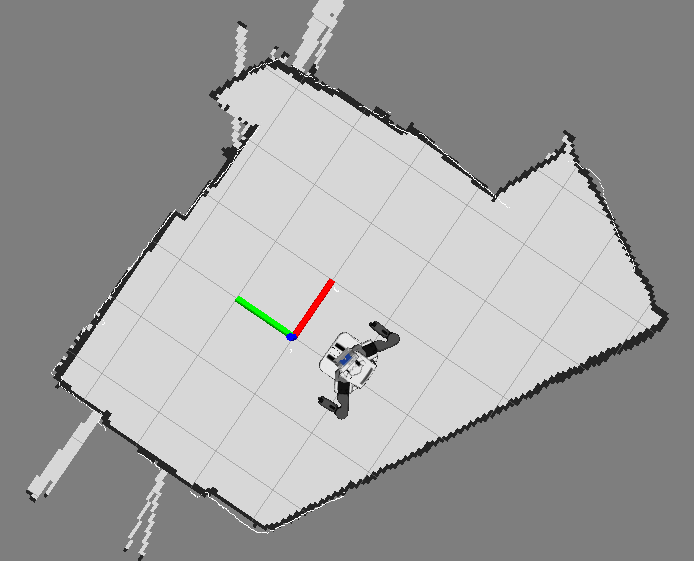
\includegraphics[width=0.59\linewidth]{./img/Map2d.png} 
  \caption {Exemple de carte pour la navigation et la localisation du robot}
  \label{fig:map}
\end{figure}

\subsection{Objets}
Les lieux de travail et de vie sont également composés d'objets diverses. Des récipients, des outils, des vétements, des appareils éléctroniques... auntant d'éléments qui peuvent prendre des formes et fonctionnalités variées.
Certains de ces objets peuvent également avoir diverses états. Par exemple, une bouteille peut être vide ou pleine, un vétement peut être propre ou sale, un appareil éléctronique peut être éteind ou allumé.
Ces objets sont pour la plupart manipulable au cours d'une interaction. Il est donc important que le robot puisse, afin d'agir corrèctement sur son environnement, reconnaître ces objets et dans la mesure du possible, connaître et suivre l'évolution de leur état.

Pour reconnaître les objets, diverses méthodes existent. Ces méthodes sont basées sur des solutions capteurs tel la stéréo vision \cite{murphy2005}
ou en utilisant un capteur RGBD tel la kinect \cite{tang2012}.
%TODO? ajouter illustration reconnaissance d'objets + image kinect
Ainsi, le robot est capable de détecter, reconnaître et positionner l'objet par rapport au reste de l'environnement.


\subsection{Proprioception et autres robots}
Pour comprendre la situation, le robot doit également pouvoir comprendre la situation des agents, à commencer par lui-même. Le robot est généralement composé de plusieurs membres, lui permettant de manipuler des objets, de changer son champs de vision ou de se déplacer. Il lui est donc nécéssaire de connaître la configuration de ses propres membres. Cette faculté est appellée proprioception. Sur les robots, des capteurs de position permettent de transmettre la configuration des articulations, et ainsi de connaître la posture globale du robot. En utilisant les éléments statiques et à l'aide de techniques de localistion,
le robot peut également estimer sa position globale par rapport aux autrés éléments de l'environnement.

\begin{figure}[ht!]
 \centering
  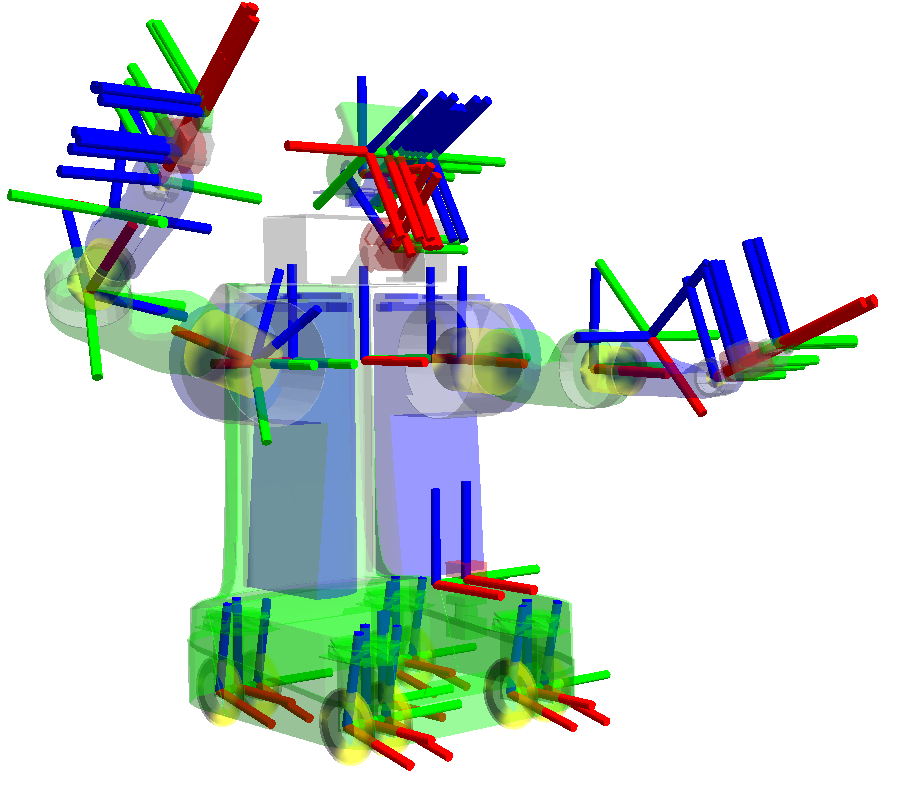
\includegraphics[width=0.59\linewidth]{./img/frames2.png} 
  \caption {Représentation tridimensionnelle du robot pr2 avec des repères pour chacune de ses articulations}
  \label{fig:frames}
\end{figure}

Dans le cas où l'interaction comporte plusieurs robots, il leur est possible de communiquer, à travers le réseau, leur configuration et ainsi permettre à chaque robot de pouvoir accéder dirèctement à leurs propres données. Grâce à cela, il est possible à chaque système robotique de connaître la position et la configuration de chaque robot par rapport à l'environnement global.


\subsection{Humains}

Lorsque un ou plusieurs humains sont présents dans l'environnement, il est essentiel pour le robot de pouvoir au moins les détecter, voir de les reconnaître.
Tout comme le robot, l'homme possède plusieurs membres. Il est donc important de connaître la position de chaque homme mais aussi sa posture, et donc de percevoir la postion de ses membres. Un capteur très utilisé pour détecter les humains est la kinect. Elle permet de connaître directement la position des différents membres de chaque humain. La figure \ref{fig:skeleton} présente la perception tridimensionnelle de la kinect et le suivi des membres de chaque humain ainsi que l'estimation de son squelette (de la position de ses membres) calculée à partir de cette perception.

%image kinect
\begin{figure}[ht!]
 \centering
  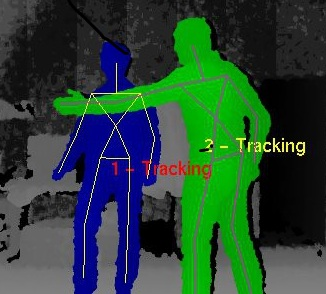
\includegraphics[width=0.59\linewidth]{./img/skeleton3.jpg} 
  \caption {Image provenant de la kinect et illustrant le suivi des humains et de leurs membres.}
  \label{fig:skeleton}
\end{figure}


De même, les équipements de capture de mouvements, tel que celles utilisées dans le cinéma d'animation, peuvent permettre d'obtenir la position et la configuration des membres des humains. Cependant cette dernière solution nécessite aux humains de s'équiper de combinaison ayant des repères visuels pour les caméras de la capture de mouvements (voir figure \ref{fig:mocap}).

%image mocap
\begin{figure}[ht!]
 \centering
  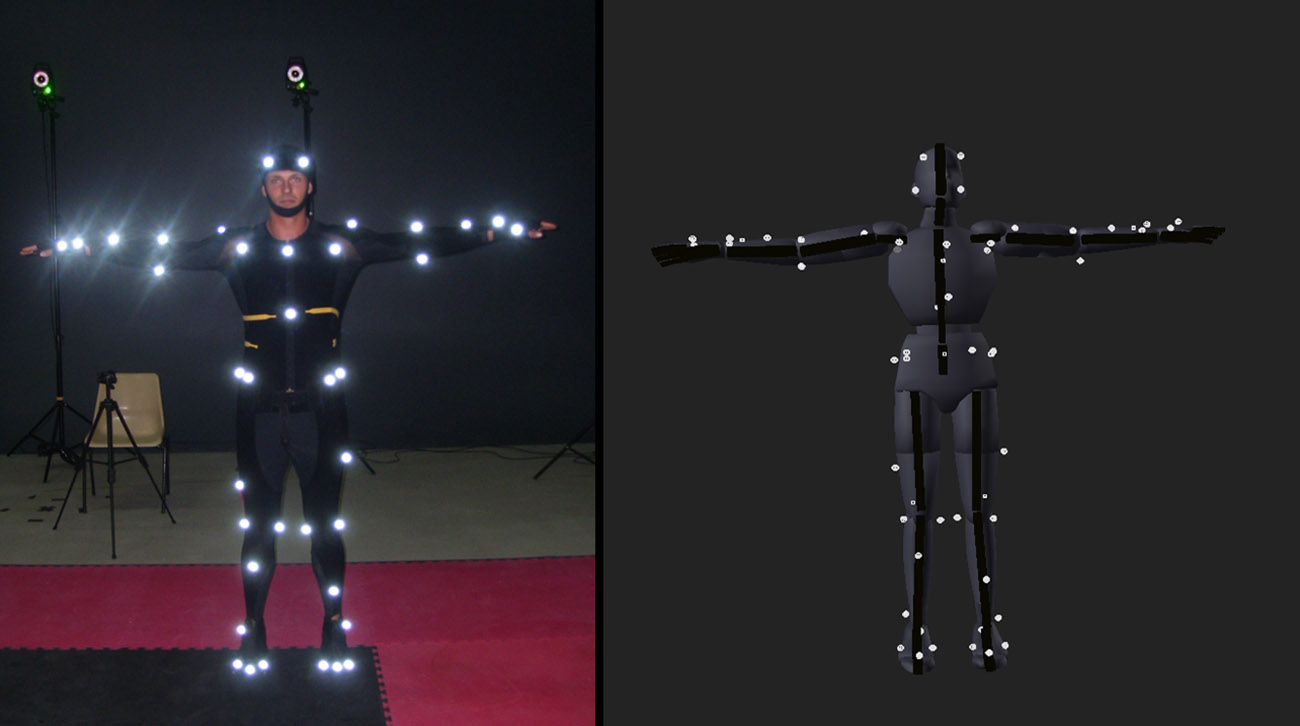
\includegraphics[width=0.69\linewidth]{./img/motionCap.jpg} 
  \caption {Exemple d'équipement de motion capture pour le suivi de l'homme et de sa posture. À gauche un homme équipé et à droite son modèle tridimensionnel.}
  \label{fig:mocap}
\end{figure}





\section{Calculs géométriques}
\label{sec:calculs}
\subsection{Modèle tridimensionnel et calculs de faits}
\label{sec:facts}

Une fois que le système robotique peut accéder aux données lui permettant d'obtenir la configuration de l'environnement et des divers éléments qui le composent, il est nécéssaire, pour en extraire les informations pertinentes, de croiser les données. Pour ce faire, il faut dans un premier temps regrouper les données de position dans un repère commun afin que le robot puisse avoir une représentation globale de la scène. La figure \ref{fig:real} illustre cette unification avec une représentation en trois dimensions des divers éléments de l'environnement tel qu'ils sont perçus par le robot.

\begin{figure}[ht!]
 \centering
  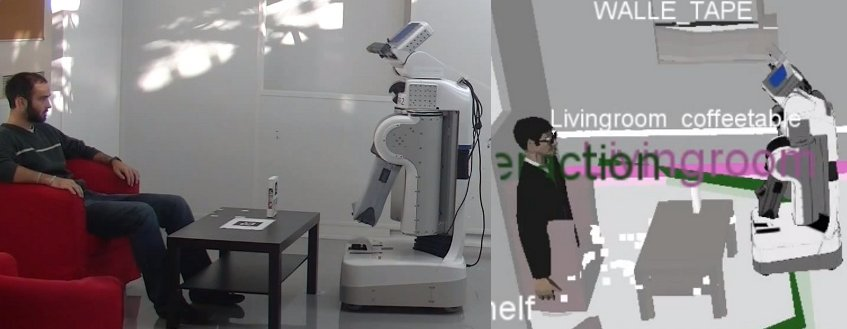
\includegraphics[width=0.99\linewidth]{./img/real.jpg} 
  \caption {Exemple d'environnement d'interaction homme robot (à gauche), et la représentation tridimensionnelle de cette même scène tel qu'elle est perçue par le robot (à droite)}
  \label{fig:real}
\end{figure}


L'unification des données capteur va permettre au système de maintenir un état du monde tridimensionnel comme dans la figure \ref{fig:real}. Pour améliorer le suivit de l'état du monde notamment au niveau des positions des divers éléments, il est parfois nécéssaire d'établir un raisonnement basé sur des hypothèses, par exemple pour éviter de perdre la position d'un objet lorsqu'il n'est plus perçu. Ces raisonnements et hypothèses reposant sur des calculs géométriques et sur l'évaluation de la situation, ils seront présentés plus tard (en section \ref{sec:hypo}). 

La construction et le maintien du modèle tridimensionnel par agrégation des données provenant des divers capteurs va permetre de générer des liens symboliques entre les différents éléments de l'environnement. Dans notre système, nous représentons l'état du monde symbolique par une liste de \textit{faits}. Un \textit{fait} est traduit par une structure de données contenant divers champs que nous allons énumérés.

\begin{itemize}
\item \textit{Subject}: le sujet sur lequel la propriété s'applique. Il peut s'agir d'un agent (humain ou robotique), d'un objet ou du membre d'un agent (e.g.: \textit{Red\_Mug}, \textit{Human1}, \textit{PR2\_ROBOT}, \textit{Human1\_Right\_Hand}).
\item \textit{Property}: la propriété attachée au sujet du fait (\textit{Subject}) (e.g.: \textit{isOn}, \textit{isFull}, \textit{isMoving}, \textit{isPointing}, \textit{canSee}).
\item \textit{Target}: il se peut que la propriété relie l'entité-sujet \textit{Subject} avec une entité-cible \textit{Target}. Par exemple, si une entité \textit{RED\_BOOK} se trouve sur une entité \textit{KITCHEN\_TABLE}, \textit{RED\_BOOK} sera alors le sujet du fait tandis que \textit{KITCHEN\_TABLE} sera la cible.
\item \textit{PropertyType}: ce paramètre définit la catégorie dans laquelle on peut classé la propriété. Il peut s'agir par exemple d'une propriété de position, d'état, de mouvement, de posture ou d'accéssibilité. En utilisant ce paramètre, lorsqu'un module extérieur ajoute un fait dont la propriété est inconnue, il reste possible de savoir quel type de propriété est décrite par ce fait. Cela permet également d'appliquer certain traitements aux faits en fonction de leur type.
\item \textit{Value}: selon la propriété, il est possible qu'une valeur y soit rattachée. Par exemple, la propriété décrivant l'état d'un containère \textit{isFull} ou le déplacement d'une entité \textit{isMoving} peuvent prendre la valeur \textit{TRUE} ou \textit{FALSE}. Un autre exemple, si on représente la distance entre deux membres, comme la main (ou pince) du robot et la tête de l'homme, le paramètre \textit{Value} peut contenir la valeur \textit{DANGER}, \textit{CLOSE} ou \textit{FAR}. Dans certains cas, il est également possible de donner une valeur numérique à ce paramètre.
Dans d'autres cas, pour représenter le manque de connaissances sur une propriété et la "conscience" de ce manque, la valeur du fait peut aussi être \textit{unknown}.
\item \textit{Confidence}: ce chiffre entre 0 et 1 représente la fiabilité du fait. Cette valeur peut être liée à la fiabilité des capteurs ou résulter du calcul de la propriété.
\item \textit{Time}: ce paramètre permets d'enregistrer le moment auquel la propriété a été calculée.
\item \textit{FactObservability}: ce dernier paramètre représente la probabilité qu'un humain aquière la connaissance du fait s'il est capable de voir le sujet du fait. Plus de détails sur ce paramètres seront donné dans le chapitre suivant.
\end{itemize}

Par exemple, le vecteur 
%TODO Make this as a table?
$<$ $Subject = Bob\_Right\_Hand$, $Property = isMovingToward$, $Target = HP\_Book$, $PropertyType = motion$, $Confidence = 0.8$, $time = 145571646570$, $FactObservability = 0.7$ $>$ représente le fait qu'à un temps \textit{time}, le bras droit de l'agent Bob (\textit{Bob\_Right\_Hand}) se dirige vers le livre "Harry Potter" (\textit{HP\_Book}).
Les séctions suivantes décrivent les raisonnements géométriques et temporels 
permettant de générer ce genre de faits.


\subsection{Zones}
\label{sec:zones}

Pour avoir une première estimation de la situation, il est possible dans un premier temps de regarder l'emplacement des divers éléments. Pour ce faire, nous utilisons des zones ayant une signification sémantique particulière pour avoir une première catégorisation de la situation en fonction de la répartition des éléments par rapport à ces zones.

Nous définissons comme zone un emplacement délimité de l'environnement ayant une signification particulière. Ces zones peuvent être bidimensionnelles ou tridimensionnelles selon l'utilisation qui en est faite. Ces zones peuvent être statiques ou dynamiques et sont paramétrables. Les paramètres permettant de définir ces zones sont:
\begin{itemize}
\item le type de la zone: ce paramètre permets de catégoriser la zone. Ainsi une zone peut-être une pièce (comme une chambre, un salon...), une zone d'interaction avec un agent (par exemple en face de l'agent en quéstion), une zone de danger...
Ce paramètre permets donc de donner un contexte sémantique à la zone concernée en l'associant à une catégorie.
\item le type d'éléments concernés par cette zone: une zone peut concerner que certains éléments de l'environnement. Ce paramètre permets de définir quel type d'éléments doivent être considérés. Il peut s'agir de toutes les entités (objets, et agents), ou simplement des agents ou d'un seul type d'entité (humain, robot ou objet). Les éléments ne faisant pas partie de la catégorie choisit seront ignorés des calculs effectués en lien avec cette zone.
\item le type de calcul lié à cette zone: ce paramètre permets de définir quels calculs doivent être fait. Ces calculs seront appliqués aux éléments concernés et se trouvant à l'intérieur de la zone.
\item le "propriétaire" de cette zone: une zone peut avoir un "propriétaire". Cela signifie que la zone sera "liée" à l'entité désignée comme propriétaire de la zone.  La position et l'orientation de la zone seront mis à jour avec la position et l'orientation de son propriétaire. Ainsi, il est possible de définir une zone d'interaction liée au robot par un trapèze positionné devant celui-ci. Si le robot bouge, la zone bougera avec lui pour toujours rester devant lui.
\end{itemize}

Pour reprendre l'exemple précédent, il est possible de définir une zone d'interaction devant le robot pour savoir si un humain se trouve dans cette zone et activé conditionnellement certains calculs, tel que l'orientation de l'humain pour savoir si celui-ci est dans une configuration permettant l'interaction.
La zone aura alors le vecteur de paramètres <\textit{interaction, humans, orientation, robot}>
Cette zone est illustrée par la figure \ref{fig:interaction} par une zone violette.
Dans l'exemple illustré, les faits (simplifiés ici) \textit{bob isInArea interaction} et \textit{bob isFacing pr2} sont générés. Le robot (\textit{pr2}) peut donc en déduire qu'il lui est dirèctement possible de parler à \textit{bob} mais pas à \textit{greg} (il devra par exemple commencer par l'appeller).


\begin{figure}[ht!]
 \centering
  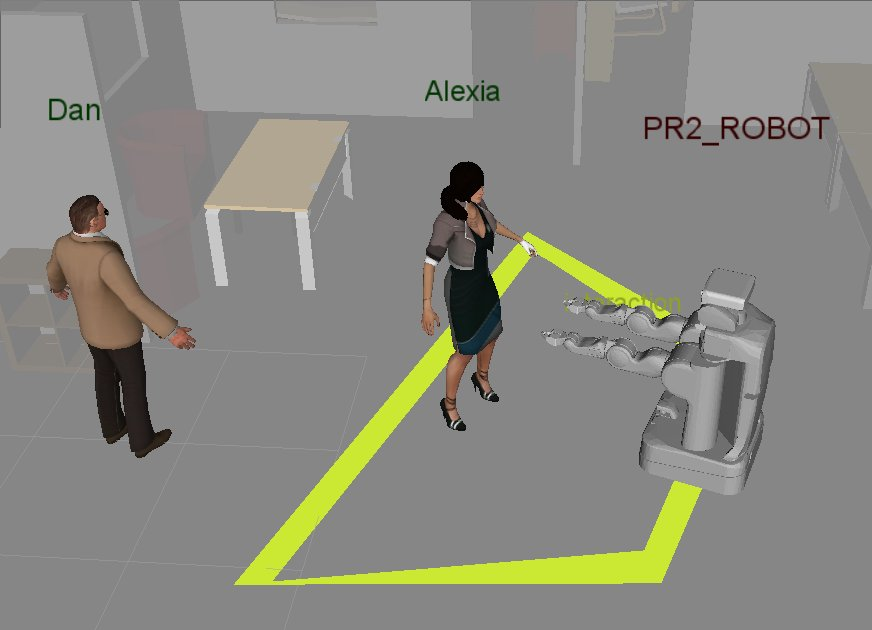
\includegraphics[width=0.69\linewidth]{./img/interactionarea.jpg} 
  \caption {Zone liée au robot pr2 pour savoir si un humain est dans sa zone d'interaction. Ici bob se trouve dans la zone, le robot va donc calculer si celui-ci lui fait face}
  \label{fig:interaction}
\end{figure}

Ces zones peuvent être créées, mises à jour et supprimées pendant l'interaction (par exemple par le superviseur) et sont utiles pour avoir une première discrimination de la situation et des calculs conditionnels.


\subsection{Agencement}
\label{sec:agencement}
Pour pouvoir passer d'une représentation numérique à une représentation symbolique de l'environnement qui entoure le robot, il est nécéssaire d'avoir, dans l'infrastructure logicielle du robot, un composant qui calcul les relations spatiales entre les objets. Ce composant fait une représentation tridimensionnelle de l'environnement en utilisant les données de position et d'orientation des différents éléments et leur mise à jour en temps réél pour tenir compte de l'état du monde courant. À partir de cette représentation 3d de l'état du monde, il calcul des propriétés d'agencement spatiale pour décrir la situation des objets.

Ce composant permets de calculer si un objet O1 se trouve au dessus d'un autre objet O2 (\textit{O1 isOn O2}), dans un objet O2 (\textit{O1 isIn O2}) ou à côté d'un objet O2 (\textit{O1 isNextTo O2}) comme illustré par la figure \ref{fig:spar}. Les détails de calculs et la méthode d'implémentation proviennent de travaux précédents et sont décrits dans \cite{sisbot2011situation}.


\begin{figure}[ht!]
 \centering
  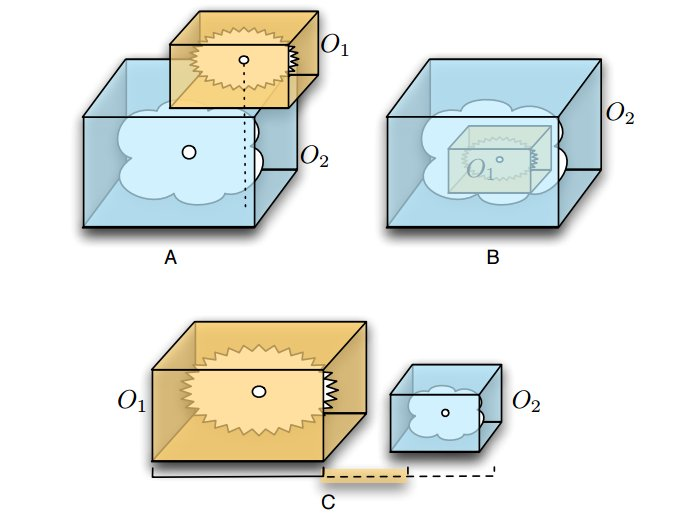
\includegraphics[width=0.5\linewidth]{./img/spar.jpg} 
  \caption {Relation spatiale entre deux objets: A) propriété \textit{isOn}, B) propriété \textit{isIn}, et C) propriété \textit{isNextTo}}
  \label{fig:spar}
\end{figure}


\subsection{Situation des agents}
\label{sec:situationAgents}

Quand le robot doit accomplir une tâche collaborative avec d'autres agents, et notamment avec des humains, il est primordial pour le système robotique d'identifier les activités humaines. Pour ce faire, nous utilisons un composant qui permet de surveiller chaque agent en utilisant des calculs de faits concernant les déplacements, la posture et la distance par rapport à certains points d'intéret.

Le composant permettant de calculer ces faits enregistre en permanance les positions des entités, et ce pour une courte période de temps (quelques secondes). Afin de pouvoir stocker ces données temporairement et de les renouvellées, nous avons créé une structure de donnée appellée buffer ciculaire temporel (time stamped circular buffer). La différence avec les buffers circulaires traditionnels est que les données y sont labellisées en fonction d'un marqueur temporel et qu'il est possible d'y accéder en utilisant le temps qui leur a été attribué. Ceci permets d'accéder à la donné de position des entités à un temps donné (moyennant de ne pas dépasser la taille du buffer).

Comme le suivi d'un agent peut s'avérer pertinant seulement dans certaines situations, le calcul des faits concernant n'importe quel agent peut être activé ou désactivé par requète. Ceci permets d'éviter de calculer en permanance des faits concernant tout les agents en ciblant seulement les agents qui se trouvent dans une situation nécéssitant un suivit particulier.
Il est également possible de faire une requête pour activer le calcul de faits concernant un ou plusieurs des membres d'un agent. Lorsque le suivit d'un agent est activé, le composant calcul le déplacement de l'agent à partir des données présentes dans le buffer circulaire associé, afin de déterminer si l'agent est en train de se déplacer. En utilisant le buffer circulaire associé à l'agent et ceux associés aux autres entités, il est possible de calculer si l'agent se déplace en diréction d'une entité en particulier (même si cette dernière est également en cours de déplacement) et l'évolution temporelle de la distance entre l'agent et un point d'intéret. Ce calcul peut être aussi bien fait sur la position globale de l'agent ou sur l'un de ses membres (par exemple sur la main de l'homme).
En plus du mouvement, nous calculons également les distances entre les agents surveillés (respectivement les membres surveillés) et les autres entités.
De cette manière il est possible de savoir si un humain, ou l'un de ses membres, est proche d'un point d'intéret (comme le robot ou un objet avec lequel il veut intéragir).
Par exemple, ce module peut générer les faits (simplifié ici) <\textit{HUMAN1 isMoving TRUE}> pour indiquer que l'humain \textit{HUMAN1} est en mouvement ou <\textit{HUMAN1\_RIGHT\_HAND isMovingToward BLUE\_BOOK}> pour indiquer que la main droite de l'humain se dirige en diréction du livre bleu.

Le dernier type de fait concerne la posture de l'agent. En utilisant le buffer circulaire il est possible de savoir vers quoi l'humain pointait le doigt à un instant donné. Ceci peut être utile par exemple pour un module de fusion d'un système de dialogue. Ainsi, si un humain demande au robot "donne moi ça", si la reconnaissance de parole est capable de fournir le temps pour lequel le mot "ça" a été prononcé, il est possible de faire une requète pour savoir quel objet était pointé par l'humain au moment où il a prononcé le mot "ça". Pour aléger la charge de calcul, ce fait est calculé seulement par requête (et non en permanance comme les autres) et renvoye une liste d'entités avec une probabilité pour chaque candidat potentiellement pointé.




\section{Hypothèses pour le maintien de l'état du monde}
\label{sec:hypo}
\subsection{Hypothèses de position}
%Put this in objects?


Dans leur quotidien, les humains sont occupés par divers activités (cuisine, nétoyage, bricolage...). Ces activités impliquent très souvent l'utilisation d'objets. Comme les robots sont fait pour assister les hommes dans leur tâches quotidiennes, il est crucial qu'ils puissent non seulement manipuler les objets, mais également suivre leur changement de position. Notre but ici n'est pas de discuter des différentes méthodes de suivi d'objet basé sur la perception mais d'expliquer comment le raisonnement sur les données de perception peut améliorer la détection et le suivi d'objet.

Localiser et suivre un objet n'est pas une tâche simple. En effet, l'objet peut être de petite taille et par conséquent être fréquement occlu ou hors du champ visuel.
Les humains sont capables de connaître la localisation d'un objet même sans perception directe. Ils font en permanance des hypothèses sur la position des objets qu'ils ne peuvent pas voir et effectuent des raisonnement basés sur ces hypothèses. Pour travailler efficacement avec des humains, le robot doit être capable lui aussi de faire ce genre de raisonnements.

Pour ce faire, nous avons ajouté au composant qui maintient l'état du monde à jour la possibilité d'émettre des hypothèses de position lorsqu'un objet n'est pas visible.

Comme hypothèse de base, lorsque le robot est dans l'incapacité de voir l'objet (l'objet est hors du champs de vision ou est occlut), le système suppose que l'objet est à la même place et a la même orientation que la dernière fois qu'il l'a perçu. Dans la figure \ref{fig:occluded} 
le livre bleu n'est pas visible par le robot (car il est caché par la boîte rose). Cela signifie que le capteur de vision n'est plus capable de fournir la donnée de position de cet objet. Cependant, le système de maintient de l'état du monde le concerve tel quel dans le modèle de l'environnement car il sait que l'objet est occlut, et qu'il est donc normal qu'il ne soit pas détecté. Cette hypothèse de maintien de position est utilisée comme hypothèse par défaut. Cela signifie que si il y a une autre hypothèse concernant la position d'un objet, nous choisirons cette dernière plutôt que celle par défaut.

\begin{figure}[ht!]
 \centering
  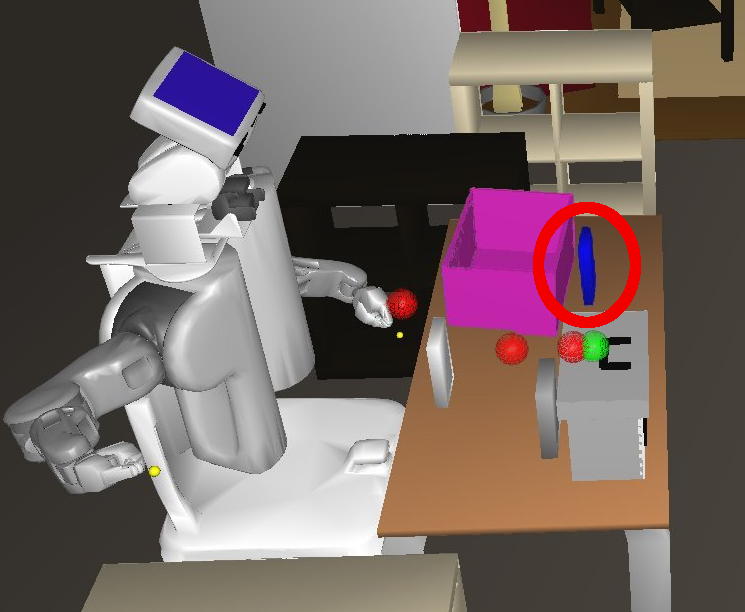
\includegraphics[width=0.69\linewidth]{./img/occluded.png} 
  \caption {Exemple d'État du monde où le système maintient les objets en position même si ils ne sont pas dirèctement perçus (comme le livre bleu).}
  \label{fig:occluded}
\end{figure}

Les autres hypothèses de position sont générées à partir des actions du robot et de l'homme. Si le robot attrape un objet, l'objet sera probablement caché par sa propre main, mais nous savons où l'objet se trouve (dans la main du robot).
Nous avons le même type d'hypothèse pour l'humain, en utilisant les observations sur la situation de l'humain (proximité avec un objet, posture, mouvement) présentés à la section \ref{sec:situationAgents}, il est possible de suivre les actions de l'homme, et ainsi de savoir quand un humain prends un objet ou le dépose.

En dernier lieu, nous avons également une hypothèse permettant de connaître la position des objets lorsque ceux-ci sont contenus dans d'autres objets.
Si un agent laisse tomber un objet dans un autre, même si il n'est pas possible de voir l'objet lâché, il est possible d'approximer sa position (par exemple en le mettant au centre du contenant).

\begin{figure}[ht!]
 \centering
  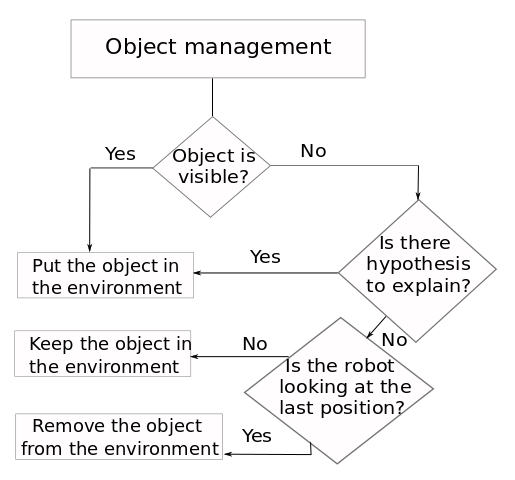
\includegraphics[width=0.70\linewidth]{./img/hypothesis.png} 
  \caption {Schema de raisonnement pour gérer la position d'un objet. Les hypothèses sur la position des objets peuvent provenir d'une occlusion, d'un objet dans un conteneur ou dans la main d'un agent.}
  \label{obj_manag_fg}
\end{figure}

Pour résumé, le robot utilise en premier lieu la perception, puis s'il n'est pas possible de percevoir l'objet il utilise des hypothèses de position.
Si aucun des deux n'est disponible, il usitile la dernière position de l'objet, comme indiqué par la figure \ref{obj_manag_fg}.
Les hypothèse de position doivent être gérées en temps réel pour maintenir un modèle du monde cohérent.
Dans le cas où un objet a une hypothèse de position et est perçu en même temps, la position perçue est comparée avec celle donnée par l'hypothèse de position. Si la  position indiquée est incompatible (distance trop importante) l'hypothèse est alors supprimée car elle est considérée comme impossible.
Si un objet devrait pouvoir être perçu et ne l'est pas, alors l'hypothèse par défaut est annulée et la position de l'objet prends alors la valeur "unknown" pour indiquer que le robot ne sait pas où se trouve l'objet en quéstion.

Ces hypothèses concernant la position des objets liées à un raisonnement top-down (symbolique vers sub-symbolique) permettent au robot d'avoir un suivi plus efficace des objets, spécialement quand ils sont occlus ou non perçus.


\subsection{Généralistion}


%TODO: généralisation du maintient du monde par la gestion des hypothèses (rempli / vide, chaud/froid...)
% Différent car ne modifi pas l'état du monde sub symbolique

Pour aller plus loin, nous travaillons actuellement à généraliser ces hypothèses. En effet, il est important de pouvoir suivre la position des objets, et donc d'établir des hypothèses pour pallier le manque de visibilité et avoir un suivi éfficace de la position des objets, mais il est également important de connaître l'état des divers propriétés liées aux objets. Contrairement aux hypothèses de positions, ces hypothèses n'influencent pas la représentation tridimensionnelle de la scéne mais uniquement les données symboliques.

Ce maintien des hypothèses concernant l'état symbolique du monde est réalisé grâce à un module de reconnaissance d'actions appellé AIR (Action and Intention Recognizer), dont le fonctionnement est présenté au chapitre \ref{chapter4}.
Ce module transmets au module de gestion d'hypothèses (Hypotheses Manager) les actions détectées par le système.
Basé sur un nombre de règles liées aux actions, le module de gestion d'hypothèse est capable de mettre à jour certaines propriétés liées à l'état symbolique du monde.

Par exemple, si le module AIR détecte qu'un humain a versé le contenu \textit{C} d'un récipient \textit{B}(comme une bouteille) dans un autre récipient \textit{V} (comme un verre), le rôle du module de gestion des hypothèses sera d'envoyer une requète à la base de données pour mettre à jour l'état des propriétés liées à \textit{V} et \textit{B}. Ainsi, la propriété \textit{isEmpty} sera mise à faux pour \textit{V} et la propriété \textit{hasLiquid} sera ajoutée avec \textit{C} comme valeur (\textit{C} peut être par exemple de l'eau. Le module de géstion d'hypothèse sera également chargé de décrémenter la quantité de \textit{C} contenue dans \textit{B}.
Pour résumer, ce module de gestion d'hypothèses permets d'appliquer les effets (ou postconditions) liées à une action lorsque celle-ci est détectée. Il sera également en charge d'assurer la cohérence globale de l'état du monde.


Le schéma \ref{fig:hypo} présente l'architecture prévisionnelle permettant cette géstion d'hypothèses. Le module de gestion d'hypothèses peut envoyer des requêtes au module d'agrégation de données et de maintien du monde (Perceived Data Gathering) pour modifier la position d'un objet, ou à la base de données temporelle (présentée à la section suivante) pour modifier certains faits, et donc l'état du monde symbolique.

\begin{figure}[ht!]
 \centering
  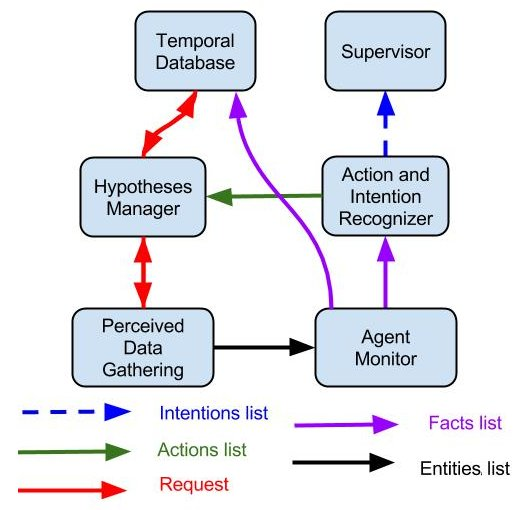
\includegraphics[width=0.7\linewidth]{./img/hypotheses_manager.jpg} 
  \caption {Schéma de l'architecture prévisionnelle pour le module de gestion des hypothèses.}
  \label{fig:hypo}
\end{figure}


%TODO: Temporal database here?
\section{Base de données temporelle}
\label{sec:db}
%%%%%%%%%%%%%%%%%%%%%%%%%%%%%%%%%%%%%%%%%%%%%%%%%%%%%%%%%%%%%%%%%%%
Nous avons présenté précédement comment divers composants contribuent à maintenir un état du monde géométrique (sub symbolique). Nous avons également présenté comment d'autres composants, à partir de l'état du monde géométrique et de raisonnements et calculs sur celui-ci, générent une liste de faits permettant une représentation symbolique de l'état du monde et une éstimation de la situation.

Afin de regrouper ces données symboliques et permettre un accès standardisé et efficace, nous avons ajouté une base de données SQL à notre système.

\subsection{Gestion des données}
\label{sec:dbd}
La base de données peut gérer deux types de données: les données statiques et dynamiques. En effet, il est possible de connaître à priori certaines informations sur l'environnement tel que la couleur, le nom de certains objets ou leur type ou leur propriétaire. 
Nous avons donc dans notre base de donées une première table permettant d'avoir des informations sur les diverses entitées de l'environnement. Cette table peut être complétée en ligne si le système reçoit des informations complémentaires durant l'interaction (si le robot découvre de nouvelles propriétés statiques ou de nouveaux objets, que se soit par la perception ou le dialogue).

Concernant les données symboliques et notamment les \textit{faits} générés par les divers composants d'évaluation de la situation, la base de données récupère en permanance la liste de faits générée et publiée par chacun des modules. Cela permet de vérifier les changements apparus dans l'environnement pour mettre à jour la table de représentation symbolique de l'état du monde tel qu'il est perçu par le robot (\textit{ROBOT\_WS\_TBL} pour Robot World State Table).
Cette table est composée de faits qui sont considérés comme vrais et mis à jours en temps réel. Ces faits proviennent des divers modules d'évaluation de la situation et ont comme valeur temporelle la date où le fait a été détecté.

%blabla etat du monde + données statiques

\subsection{Gestion de la temporalité}
\label{sec:dbt}
L'une des valeurs ajoutées de cette base de données est l'aspect temporel.
En effet, lors d'une interaction homme robot, de nombreux événements peuvent se succéder et pour pouvoir comprendre et interpréter les actions et les élocutions de l'homme, il est important de considérer l'historique de l'interaction.

Nous avons donc ajouté une géstion de l'aspect temporel.
Pour ce faire, lorsqu'un fait est considéré comme vrai à partir d'un temps t1 et donc présent dans la table de représentation symbolique de l'état du monde perçu par le robot, le temps t1 lui est attribué jusqu'à ce que ce fait soit considéré comme faux à un temps t2.

Lorsque le fait est considéré comme faux en t2, ou lorsqu'il change de valeur, il est retiré de la table \textit{ROBOT\_WS\_TBL} pour être mis dans une table mémoire \textit{ROBOT\_MEM\_TBL}. Cette table contient également une liste de faits. À la différence de la table \textit{ROBOT\_WS\_TBL}, les faits de cette table peuvent être en double (deux faits identiques peuvent être présent dans la table si ils ont des temps différents) et représentent des faits passés. Pour ce qui est du temps associé, chaque fait a deux dates: la date t1 à laquelle le fait a commencé a être vrai (ou plutôt détecté comme étant vrai) et la date t2 à laquelle le fait a céssé d'être vrai (détecté comme étant faux).
Pour avoir un accés direct aux transitions, nous avons également ajouté une table d'événements \textit{EVENT\_TBL}. Lorsqu'une transition de fait est detectée (un fait n'est plus vrai ou change de valeur), en plus de le retirer de la table de faits courant et de l'ajouter à la table mémoire, nous ajoutons la transition avec la date de t2. 

Pour illustrer, nous prenons l'exemple où un homme \textit{H} prends un objet \textit{O} sur une table \textit{T} à un moment t2. Trois opérations seront faites dans la base de données:

\begin{itemize}
\item Le fait \textit{O isOn T} sera déplacé de la table \textit{ROBOT\_WS\_TBL} vers la table \textit{ROBOT\_MEM\_TBL}, avec t2 comme temps de fin.
\item Le fait  \textit{H hasInHand O} sera ajouté à la table \textit{ROBOT\_WS\_TBL} avec un temps t2.
\item L'événement \textit{H picks O} sera ajouté à la table \textit{EVENT\_TBL}.
\end{itemize}

Cette gestion du temps, des événements et de la mémoire permets de pouvoir réaliser des raisonnements temporels complexes sur les données symboliques et les liens temporels entre les différents faits. L'une des améliorations à venir est de permettre "d'oublier" les événements en fonction de leur date et de leur ancienneté pour éviter de saturer la mémoire dans le cas d'une utilisations longue durée.



% %TODO: improve clearness
% Another capacity of the database component is the event based time management. This provides memory to the system.
% When facts are received, the time of detection is present in one of their variables (as mentioned in \ref{sec:facts}). When the database manager detects a shift in a property, it updates the belief tables as explained in previous section, but it also records the event. To do so, we add a table filled with each event that occurs, recording the time when the property changes. As an example, if a Mug was on a table and the robot detects that the Mug is now in Bob's hand, it will remove the fact $<$\textit{Mug isOn $Kithen\_Table$}$>$ from the belief tables of agents able to perceive the change, and add the event $<$\textit{Bob pickUp Mug}$>$ in the event table.
% In addition to the event table, we add a memory table for each agent. This memory table stores facts that the agent has believed to be true. We use as starting time the time when the agent noticed a property, and as ending time the moment when the agent detects a change in it.
% One of the application can be to 
% %find correct terminology: reference finding? grounding? desambiguate?
% %Miki: This is quite nice actually. What about making real experiments on that? XD
% %Greg: Yep, we should! I put it in the conclusion
% %But we also have to work on robustifying the thing...
% understand when a human asks "Where is the mug that was on the table" by detecting in his memory table which mug she/he is talking about and looking in the current fact table where it currently is. In addition, the robot could even tell the related event that created the change: "It is now in the sink, Bob picked it up 5 minutes ago".



%%%%%%%%%%%%%%%%%%%%%%%%%%%%%%%%%%%%%%%%%%%%%%%%%%%%%%%%%%%%
\section{Implémentation}

Les composants décrits précédement ont été implémentés dans une infrastructure logicielle open-source appelée TOASTER\footnote{TOASTER est disponible sur github à l'adresse https://github.com/Greg8978/toaster} (Tracking Of Agents and Spatio-TEmporal Reasonning).

L'un des avantages de TOASTER repose sur sa généricité et son adaptabilité grâce à une conception modulaire qui permets également d'étendre facilement l'infrastructure. En effet, comme présenté en section \ref{sec:collecte}, les données d'environnement peuvent parvenir de divers capteurs.

\subsection{Collecte de données et généricité}
\label{sec:PDG}
Pour que l'infractructure logicielle soit utilisable avec n'importe quelle configuration de capteurs, un premier module permets de collecter toutes les données et de les mettre au format TOASTER. Tous les autres modules utiliseront en suite l'état du monde au format exporté par ce module. Ce module chargé de collecté les données des divers capteurs est appellé \textit{PDG} pour Perceived Data Gathering.
Il permets à l'heure actuelle de gérer quatre types d'entrées pour l'homme, deux pour les objets, deux modèles de robot. Il gère également deux types de messages d'entrée: le ROS\footnote{http://www.ros.org/} et le pocolibs\footnote{https://www.openrobots.org/wiki/pocolibs}.

Un autre avantage de ce module est également sa simplicité d'extension. Ainsi, grâce au système d'héritage du C++ il est possible d'ajouter une entrée capteur pour détecter des objets, pour suivre l'homme ou un modèle de robot en seulement 50 à 200 lignes de code C++ (estimation basée sur les entrées déjà existantes).
Au démarrage du module ou à tout moment de l'interaction, il est possible de (re)configurer se module pour modifier les entrées à prendre en compte.

Durant la phase de développement de nouvelles fonctionnalités il est coûteux d'un point de vue matériel tout comme d'un point de vue temporel de faire des tests dans le monde réel. Pour permettre de tester rapidement et sans monopoliser de plateforme robotique, le module \textit{PDG} peut prendre en entrée des données de simulateur robotique tel que Gazebo\footnote{http://wiki.ros.org/gazebo} pour la configuration du robot, MORSE\cite{echeverria11} pour la configuration de l'homme, du robot et la vision des objets. En plus de ces simulateurs, un module intégré à TOASTER pour créer et tester des environnements d'interaction homme robot appelé \textit{toaster\_simu} a été créé. \textit{PDG} permets également d'avoir une configuration hybride.
Par exemple, il est possible d'utiliser les capteurs d'un robot réel ainsi que la détection d'objets dans le monde réel et de simuler le déplacement d'un humain (avec l'interface clavier).
Le module \textit{PDG} permets donc une grande flexibilité dans la configuration des données d'entrées. En exportant l'état du monde dans un format unique et invariable, \textit{PDG} permets aux autres modules TOASTER de s'abstraire de cette diversité et de conserver les mêmes formes de raisonnement, indépendament de la configuration des capteurs et des données d'entrées de TOASTER.

\subsection{Outils de développement}
Pour aider au développement de nouvelles fonctionnalités et à la configuration de scénarios, un module de visualisation a été ajouté à l'infrastructure TOASTER. Ce module utilise le rviz\footnote{http://wiki.ros.org/rviz} pour afficher les différents éléments en trois dimension, ce qui permets de comprendre la situation en affichant l'état du monde. Chaque entité est associée à un modèle 3D qui est positionné dans un environnement virtuel à la position et à l'orientation donnée par le module PDG. Le module affiche également les noms de chaque entités au dessus de leur modèle 3D. 
Le module permets également d'afficher les différentes zones présentes dans le module de géstion de zone (\textit{area\_manager}) avec leurs noms, comme présenté sur la figure \ref{fig:interaction}.
Concernant les faits exportés par le module de suivi d'agents (\textit{agent\_monitoring}), afin d'éviter la surcharge de l'interface, le fait \textit{isMoving} rends l'affichage du nom de l'agent plus intense selon si le système considère qu'il bouge. La donnée numérique de sa vitesse associé à ce fait permets également de faire varier cette intensité. Pour le fait \textit{isMovingToward}, une flèche reliant l'agent à l'entité vers laquelle il se déplace est tracée. L'intensité de la couleur de cette flèche varie également en fonction de l'indice de confiance du fait associé. Ce retour visuel est illustré par un exemple à la figure \ref{fig:moving}

\begin{figure}[ht!]
 \centering
  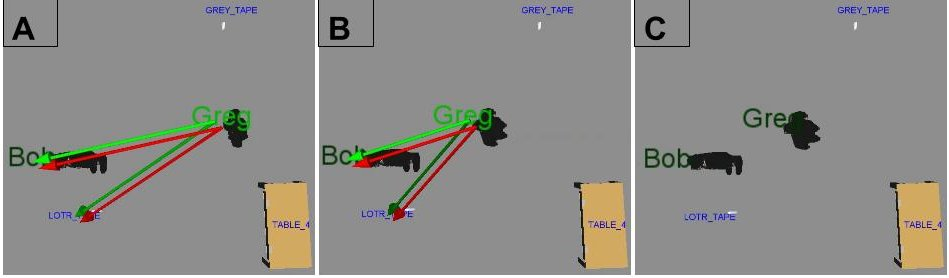
\includegraphics[width=1.0\linewidth]{./img/movingToward.jpg} 
  \caption {Affichage dans rviz des faits liés au module \textit{agent\_monitoring}. La flèche rouge indique ce fait calculer en terme de différentiel de distance alors que la flèche verte indique ce même fait en terme de diréction de trajéctoire. Sur l'image A et B \textit{Greg} se déplace vers \textit{Bob} ainsi que vers un objet (\textit{LOTR\_TAPE}). Sur l'image A et de façon plus prononcé sur l'image B, les flèches allant vers \textit{LOTR\_TAPE} sont plus sombre, indiquant que la confidence pour ce candidat est moins grande que pour \textit{Bob}. En C Greg c'est arrêté. Les flèches de diréctions sémantiques ont disparues et le nom de Greg s'est assombri (pour devenir comme celui de Bob qui est immobile).}
  \label{fig:moving}
\end{figure}

Cette visualisation permets de comprendre l'état du monde tel qu'il est perçu par le robot et permets donc de faciliter les explications liées aux agissement du robot, mais aussi de faciliter la configuration d'une nouvelle experimentation et la recherche d'erreurs lors de l'implémentation de nouvelles fonctionnalités. 

%It uses the position of the entities published by the data gathering component and the areas published by the area manager component as shown in Fig.~\ref{fig:simu} and Fig.~\ref{fig:spencer}. In a future work, we would like to improve this visualization by adding the rendering of other facts, such as the one generated by the agent monitoring component.

Un autre composant déjà évoqué dans la partie \ref{sec:PDG}, permettant de rapidement paramétrer et tester des expérimentations est le module de test \textit{toaster\_simu}. Grâce à ce module, il est possible par une simple requète d'ajouter et positionner des entités dans l'environnement. Il est également possible de contrôler ces entités par une interface clavier. Le module exportera alors en temps réel les données liées à l'état du monde créé par l'utilisateur et ces données seront lues par le module PDG. Il est donc possible, à partir d'un simple script envoyant quelques requêtes, de configurer un environnement d'interaction avec des robots, des humains et des objets. Des scripts python pour configurer un environnement de simulations sont disponibles à titre d'exemple\footnote{https://github.com/Greg8978/toaster-scripts}.


\subsection{Architecture globale}
Les autres modules compris dans l'infrastructure logicielle TOASTER ont une implémentation qui suit les descriptions données précédement.
Ainsi, le module \textit{area\_manager} permets d'ajouter et de supprimer des zones dans l'environnement à l'aide de requètes. Le modèle et les raisonnements faient dans ce module suivent la description faites en \ref{sec:zones}. Pour le calcul de l'agencement des différents éléments, un module nomé \textit{SPAR} (pour SPAtial Reasonning) est utilisé. Enfin, pour le suivi des agents décrit en \ref{sec:situationAgents}, le module \textit{agent\_monitoring} a été développé.
Concernant la base de données temporelle, nous avons conçu celle-ci en utilisant la bibliothèque SQLite\footnote{https://www.sqlite.org/}. Ce choix a été fait car cette base de données est très répendue, respecte les conventions SQL et permets une gestion in-memory des données qui augmente les performances en terme de vitesse d'accès à la donnée.

Chacun de ces modules peut être démarré et arrêter à n'importe quel moment de l'interaction. Il peut également recevoir des requètes ou des messages provenant d'autres composants mais ne dépends pas diréctement des autres. Par exemple, il est possible d'utiliser le module de raisonnement sur les zones (\textit{area\_manager}) sans \textit{PDG}. Cependant il est nécéssaire, si l'on veut que les zones calcul la présence d'entité, que le module \textit{area\_manager} reçoive les données correspondantes.
De même, la base de données temporelle a été conçue pour pouvoir lire des listes de faits en entrée mais il est possible de paramétrer celle-ci afin de définir quels listes de faits doivent être lues.
Ceci permets de facilement remplacer un module de l'architecture sans impacter les autres modules, dans la mesure où ce nouveau module respecte les conventions de formats de données d'entrée et sortie.

Pour aider à la compréhension, nous proposons le schéma d'architecture \ref{fig:toasterArch} qui présente comment les données des différents composant peuvent s'interfacer.


\begin{figure}[ht!]
 \centering
  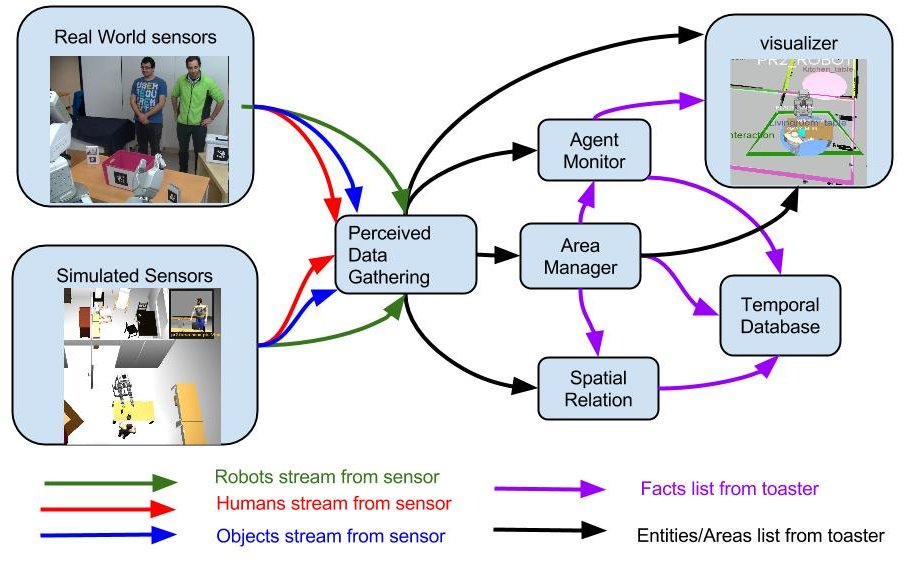
\includegraphics[width=0.99\linewidth]{./img/toasterArch.jpg} 
  \caption {Architecture de l'infractructure logicielle TOASTER avec les différents flux d'échange de données}
  \label{fig:toasterArch}
\end{figure}

\section{Résultats expérimentaux}
Pour illustrer l'utilisation possible de TOASTER, nous présentons ici deux experimentations utilisant l'infrastructure logicielle.

\subsection{Le robot guide}

L'une des premières applications de TOASTER a été de l'utiliser comme composant d'estimation de la situation pour un robot guide adaptatif, proactif et prenant en compte les humains \cite{fioreicsr2015}.

Pour cette application, le robot doit guider un groupe d'utilisateurs à travers une une zone de transite (potentiellement bondé), pour les amener à l'endroit choisit.
L'un des défis de ces travaux était de guider les personnes de façon sociallement acceptable et en prenant en compte le confort des usagers.
Pour ce faire, le robot adapte sa vitesse au groupe, ce afin de tous les amener à leur destination avec une allure qui satisfasse la plupart des usagers et évite que certains utilisateurs n'abandonnent.

Pour atteindre ces objectifs, nous avons utilisé: (1) le module PDG pour regrouper les données capteurs afin de générer et maintenir le modèle de l'état du monde; (2) les faits générés par le module de géstion des zones (area\_manager); (3) les faits générés par le module de suivi des agents (agent\_monitoring), pour comprendre la situation du groupe. 

Concernant le module de géstion des zones, deux types de zones ont été crées: les zones de guidage et les zones d'activité. Les premières sont liées au robot et évoluent donc avec sa position et son orientation. Elles sont utilisées pour évaluer la configuration des utilisateurs par rapport au robot guide, ce qui lui permet d'adapter sa vitesse en fonction de la configuration du groupe.
L'idée est de créer trois zones de guidage autour du robot pour savoir si la configuration des utilisateur indique qu'ils souhaitent que le robot aille plus vite ou si l'un d'entre eux a du mal à suivre.
Les trois zones sont appelées \textit{slow}, \textit{following} et \textit{pushing} et sont configurées comme indiqué dans la figure \ref{fig:spencer}.
L'idées est que, (1) si l'un des membres du groupe est dans la zone \textit{slow} (loin du robot) le robot \textit{ralentit}. (2) Si 1) est faux et la majorité du groupe est dans la zone \textit{pushing} (proche ou sur les côtés du robot) le robot \textit{accélère}. (3) Si 1) et 2) sont fausses, signifiant qu'à la fois aucun humain ne se trouve dans la zone \textit{slow} et que la majorité des humains se trouvent dans la zone \textit{following}, le robot \textit{continue} avec la même allure.

Le deuxième type de zones est statique, lié à une position de l'environnement, et déclenche des calculs sur les humains s'y trouvant. Ces calculs concernent les distances, le mouvement et l'orientation par rapport à un point d'intéret (comme par exemple un écran). En utilisant ces zones, le système peut détecter l'activité humaine (par exemple que l'humain regarde un écran d'information ou l'humain se dirige vers les toilettes). Cette estimation de la situation donne au robot la capacité de détecter quand un ou plusieurs des humains du groupe guidé, est investi dans une activité temporaire. Le robot peut en suite distinguer entre les situations où il devrait abandonner le guidage de certains usagers de situations où il devrait attendre les humains, voir même les aider de façon pro-active (par exemple proposer des informations s'il détecte qu'un humain regarde un panneau d'informations).

%This situation assessment gives, to the robot, the capacity to detect that one or more of the human followers are involved in a temporary activity. The robot can then disambiguate between situation where it should give up on guiding and situation where it should wait for the humans, or even proactively help the humans involved in the activity.

%TODO: rewrite to adapt to toaster
%To be relevant, reasoning on humans should be linked to the environment. The system is able to create activity areas in the environment and link them to different kind of computations. An activity area is a polygonal or circular area, which can be fixed or linked and updated with an entity's (object, human or robot) position. For now, we studied and experimented different activity areas: a) Information Screen Area, linked to information screens present in the environment; b) Touristic Point Area, linked to interesting attractions in the environment.
%Using these areas, the system can detect human activities (e.g. human is looking at an information screen, human is looking at an attraction).


%
%We believe that to be socially acceptable, the robot should adapt its speed to the group. By setting its own pace at the start of the scenario the robot  would risk of being too slow, annoying the users, or too fast, which would lead the robot to constantly stop to wait for the group, producing an awkward behavior.

%The robot defines a desired range of distance $r$ from the group. The distance of the  members of the group from $r$ will influence its actions. 1) If there is a member of the group farther than $r$ the robot will \textit{decelerate}. The main goal of a guide robot should still be guiding all of the group, and so the robot will give priority to people that would like a slower speed. 2) If 1) is false, and the majority of the group is closer to the robot than $r$, the robot will $accelerate$. 3) If 1) and 2) are false, the robot will continue at its pace.


%In some situation, the robot needs to suspend the task, because the group has stopped following it. In this case, the robot should estimate if this suspension of the collaborative scenario is temporary or permanent, and in the latter case abandon the task. We estimate this information using the Suspend Model and the activity areas from Situation Assessment. We link activity areas to the maximum time we expect that the group will be involved in the linked activity, and with a set of proactive actions that the robot can choose to execute.

%In this paper, we investigated a single possible proactive behavior: giving information. In this case, if we detect that one or more  members
%of the group has stopped following because it is looking at a touristic sight, or at an information screen, the robot can try to engage him and offer related information. At the moment, we just propose a simple routine-based framework for this behavior, and plan to further study it in the future. We believe that the solution of this problem could be rich, and that the robot should estimate the reaction of the group during the execution of its proactive behavior, in order to be able to interrupt if the group doesn't want to be helped or to resume the original task if they are satisfied by the robot's actions.

 \begin{figure}[ht!]
 \centering
 \begin{tabular}{cc}
   \vspace{-5pt}
  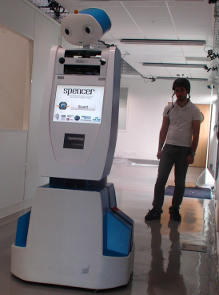
\includegraphics[width=0.4\textwidth]{img/spencer_guidingShrink.png} &
  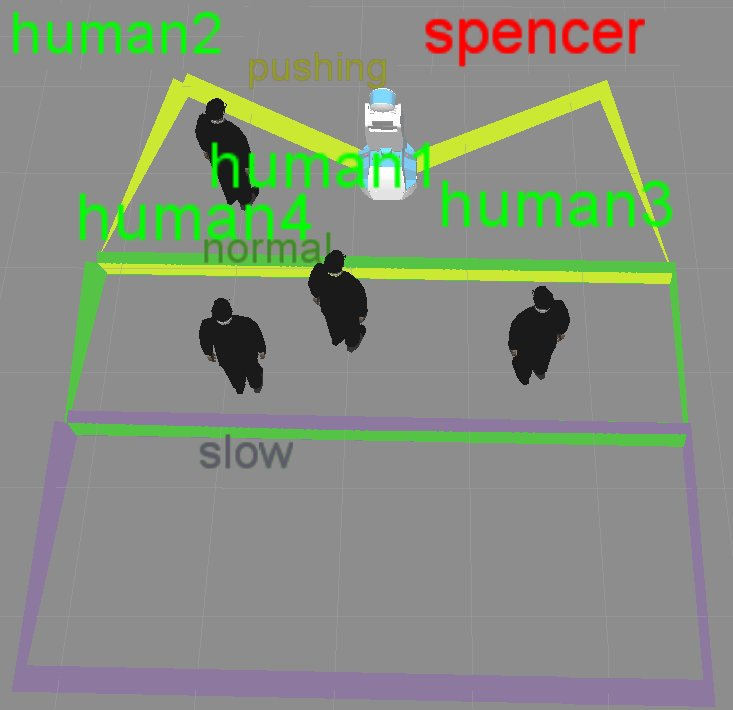
\includegraphics[width=0.56\textwidth]{img/toaster_spencer.jpg}
 \end{tabular}
 \caption{Le robot Spencer, dans le monde réel (à gauche) et dans TOASTER (à droite) avec les zones qui lui sont attachées pour guider les humains.}
 \label{fig:spencer}
  % \vspace{-10pt}
 \end{figure}
 
 
\subsection{Le robot coéquipier}
L'un des autres projets utilisant l'infrastructure logicielle TOASTER viseait à construire un robot pour travailler avec un humain sur une chaîne d'assemblage.
Dans ce scénario, le robot partage l'espace de travail avec un humain. Par conséquence, il est essentiel de pouvoir estimer à tout moment la situation spatiale de l'homme et son activité.
Le système se repose sur le module \textit{PDG} de TOASTER pour regrouper les données depuis les capteurs et construire le modèle d'environnement.
Il utilise également le module \textit{SPAR} pour avoir une représentation symbolique de l'état du monde, le module de géstion des zones pour savoir à quelle station de travail l'humain se trouve et le module de suivit des agents pour estimer l'action courante de l'homme.
En utilisant les faits provenant de ces modules, lui procurant une représentation symbolique de l'état du monde et de la situation de l'interaction, le robot est capable d'adapter son comportement à l'humain avec lequel il collabore.
La première façon d'utiliser les informations de TOASTER est d'assurer la sécurité en arretant le déplacement du robot lorsque l'homme est dans la même zone de travail et lorsqu'il est en train de se déplacer.
Un autre moyen de s'adapter est de transmettre la représentation symbolique  de l'état du monde (l'ensemble des faits) à un planificateur afin d'aider l'homme de façon proactive. En effet, avec la connaissance de l'état du monde actuel, relié à la compréhension de l'activité de l'homme, le robot peut estimer l'étape actuelle du plan à accomplir et agir afin d'aider l'homme pour les étapes suivantes du plan. Par exemple, lorsque l'homme est en train de nettoyer une pièce à assembler, si l'étape suivante est de visser cette pièce, le robot peut apporter la visseuse à l'homme. L'image \ref{fig:saphari} illustre la situation où le robot detecte que l'homme tends le bras et est orienté en direction du robot. En utilisant ces faits, le robot suppose que l'homme est prêt à recevoir l'objet et le lui donne.

%Add TOASTER image?

 \begin{figure}[ht!]

 \centering
 \begin{tabular}{cc}
  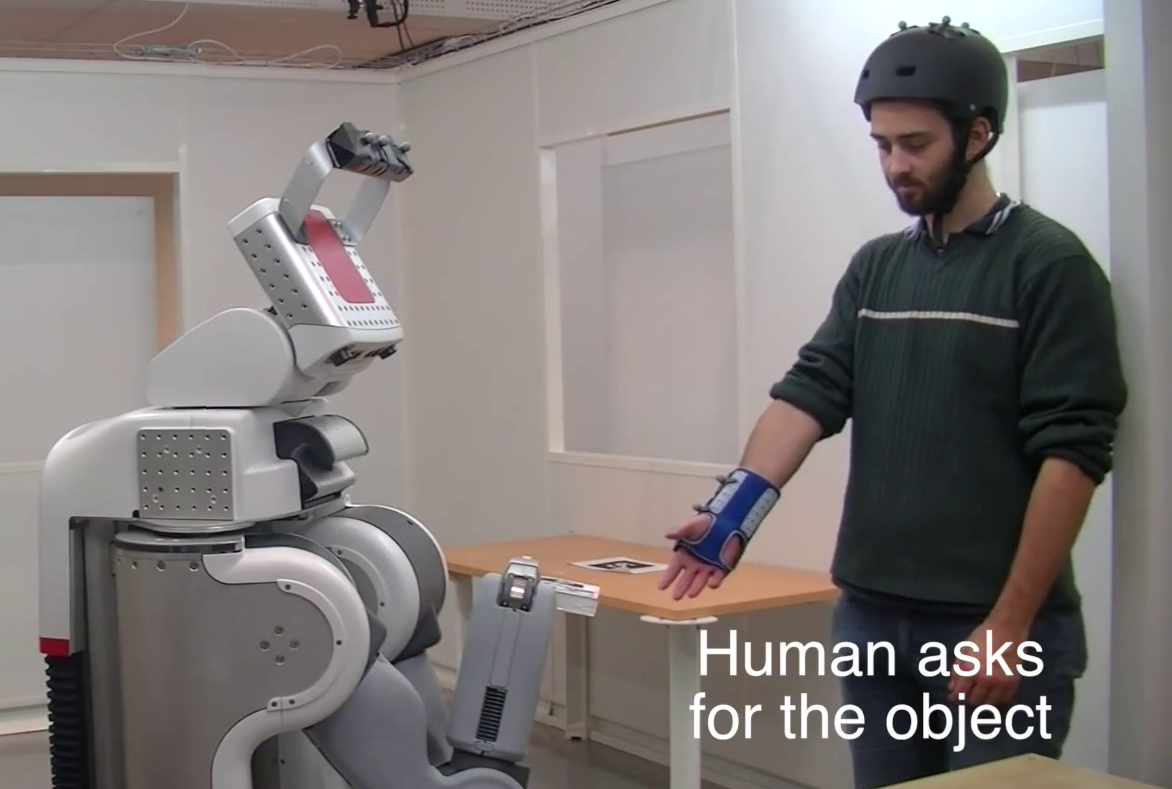
\includegraphics[width=0.7\textwidth]{img/sapharishrink.png}
 \end{tabular}
 \caption{Le robot detecte que l'homme demande l'objet en utilisant la posture de l'homme reconnue par le module de suivi d'agent de TOASTER. Ici, un système de capture de mouvement est utilisé pour suivre les positions de la tête et du bras de l'homme.}
 \label{fig:saphari}
  \vspace{-15pt}
 \end{figure}
 
 
 Ces deux exemples d'utilisation de l'infrastructure logicielle dans deux projets différents illustrent la généricité, la simplicité de reconfiguration grâce à l'architecture modulaire, ainsi que la polyvalance de TOASTER. Dans ces deux projets d'interaction homme robot, les faits générés par TOASTER ont permis de fournir les informations nécéssaires à la couche décisionnelle pour pouvoir s'adapter à l'homme et donner un comportement sociallement acceptable au robot.

%\section{Gestion de l'Incertitude}
%TODO?
%humain prends un objet dans panier à 2 objets
%-> 50 / 50?
% 
%\section{Bilan}



\ifdefined\included
\else
\bibliographystyle{acm}
\bibliography{bibliorachid}
\end{document}
\fi

\ifdefined\included
\else
\documentclass[a4paper,11pt,twoside]{StyleThese}
\usepackage{amsmath,amssymb}             % AMS Math
\usepackage[french]{babel}
\usepackage[utf8]{inputenc}
\usepackage[T1]{fontenc}
\usepackage{tabularx}
%\usepackage{tabular}
\usepackage{multirow}


\usepackage[tight,footnotesize]{subfigure}
\usepackage{algorithm} %To allow algorithm environment
\usepackage{algpseudocode} %Provides algorithmic environment

\usepackage{hhline}
\usepackage[left=1.5in,right=1.3in,top=1.1in,bottom=1.1in,includefoot,includehead,headheight=13.6pt]{geometry}
\renewcommand{\baselinestretch}{1.05}

% Table of contents for each chapter

\usepackage[nottoc, notlof, notlot]{tocbibind}
\usepackage[french]{minitoc}
\setcounter{minitocdepth}{2}
\mtcindent=15pt
% Use \minitoc where to put a table of contents

\usepackage{aecompl}

% Glossary / list of abbreviations

\usepackage[intoc]{nomencl}
\renewcommand{\nomname}{Liste des Abréviations}

\makenomenclature

% My pdf code

\usepackage{ifpdf}

\ifpdf
  \usepackage[pdftex]{graphicx}
  \DeclareGraphicsExtensions{.jpg}
  \usepackage[a4paper,pagebackref,hyperindex=true]{hyperref}
  \usepackage{tikz}
  \usetikzlibrary{arrows,shapes,calc}
\else
  \usepackage{graphicx}
  \DeclareGraphicsExtensions{.ps,.eps}
  \usepackage[a4paper,dvipdfm,pagebackref,hyperindex=true]{hyperref}
\fi

\graphicspath{{.}{images/}}

%nicer backref links
\renewcommand*{\backref}[1]{}
\renewcommand*{\backrefalt}[4]{%
\ifcase #1 %
(Non cité.)%
\or
(Cité en page~#2.)%
\else
(Cité en pages~#2.)%
\fi}
\renewcommand*{\backrefsep}{, }
\renewcommand*{\backreftwosep}{ et~}
\renewcommand*{\backreflastsep}{ et~}

% Links in pdf
\usepackage{color}
\definecolor{linkcol}{rgb}{0,0,0.4} 
\definecolor{citecol}{rgb}{0.5,0,0} 
\definecolor{linkcol}{rgb}{0,0,0} 
\definecolor{citecol}{rgb}{0,0,0}
% Change this to change the informations included in the pdf file

\hypersetup
{
bookmarksopen=true,
pdftitle="Évaluation de la sécurité des équipements grand public connectés à Internet",
pdfauthor="Yann BACHY", %auteur du document
pdfsubject="Thèse", %sujet du document
%pdftoolbar=false, %barre d'outils non visible
pdfmenubar=true, %barre de menu visible
pdfhighlight=/O, %effet d'un clic sur un lien hypertexte
colorlinks=true, %couleurs sur les liens hypertextes
pdfpagemode=None, %aucun mode de page
pdfpagelayout=SinglePage, %ouverture en simple page
pdffitwindow=true, %pages ouvertes entierement dans toute la fenetre
linkcolor=linkcol, %couleur des liens hypertextes internes
citecolor=citecol, %couleur des liens pour les citations
urlcolor=linkcol %couleur des liens pour les url
}

% definitions.
% -------------------

\setcounter{secnumdepth}{3}
\setcounter{tocdepth}{2}

% Some useful commands and shortcut for maths:  partial derivative and stuff

\newcommand{\pd}[2]{\frac{\partial #1}{\partial #2}}
\def\abs{\operatorname{abs}}
\def\argmax{\operatornamewithlimits{arg\,max}}
\def\argmin{\operatornamewithlimits{arg\,min}}
\def\diag{\operatorname{Diag}}
\newcommand{\eqRef}[1]{(\ref{#1})}

\usepackage{rotating}                    % Sideways of figures & tables
%\usepackage{bibunits}
%\usepackage[sectionbib]{chapterbib}          % Cross-reference package (Natural BiB)
%\usepackage{natbib}                  % Put References at the end of each chapter
                                         % Do not put 'sectionbib' option here.
                                         % Sectionbib option in 'natbib' will do.
\usepackage{fancyhdr}                    % Fancy Header and Footer

% \usepackage{txfonts}                     % Public Times New Roman text & math font
  
%%% Fancy Header %%%%%%%%%%%%%%%%%%%%%%%%%%%%%%%%%%%%%%%%%%%%%%%%%%%%%%%%%%%%%%%%%%
% Fancy Header Style Options

\pagestyle{fancy}                       % Sets fancy header and footer
\fancyfoot{}                            % Delete current footer settings

%\renewcommand{\chaptermark}[1]{         % Lower Case Chapter marker style
%  \markboth{\chaptername\ \thechapter.\ #1}}{}} %

%\renewcommand{\sectionmark}[1]{         % Lower case Section marker style
%  \markright{\thesection.\ #1}}         %

\fancyhead[LE,RO]{\bfseries\thepage}    % Page number (boldface) in left on even
% pages and right on odd pages
\fancyhead[RE]{\bfseries\nouppercase{\leftmark}}      % Chapter in the right on even pages
\fancyhead[LO]{\bfseries\nouppercase{\rightmark}}     % Section in the left on odd pages

\let\headruleORIG\headrule
\renewcommand{\headrule}{\color{black} \headruleORIG}
\renewcommand{\headrulewidth}{1.0pt}
\usepackage{colortbl}
\arrayrulecolor{black}

\fancypagestyle{plain}{
  \fancyhead{}
  \fancyfoot{}
  \renewcommand{\headrulewidth}{0pt}
}

%\usepackage{MyAlgorithm}
%\usepackage[noend]{MyAlgorithmic}
\usepackage[ED=MITT - STICIA, Ets=INP]{tlsflyleaf}
%%% Clear Header %%%%%%%%%%%%%%%%%%%%%%%%%%%%%%%%%%%%%%%%%%%%%%%%%%%%%%%%%%%%%%%%%%
% Clear Header Style on the Last Empty Odd pages
\makeatletter

\def\cleardoublepage{\clearpage\if@twoside \ifodd\c@page\else%
  \hbox{}%
  \thispagestyle{empty}%              % Empty header styles
  \newpage%
  \if@twocolumn\hbox{}\newpage\fi\fi\fi}

\makeatother
 
%%%%%%%%%%%%%%%%%%%%%%%%%%%%%%%%%%%%%%%%%%%%%%%%%%%%%%%%%%%%%%%%%%%%%%%%%%%%%%% 
% Prints your review date and 'Draft Version' (From Josullvn, CS, CMU)
\newcommand{\reviewtimetoday}[2]{\special{!userdict begin
    /bop-hook{gsave 20 710 translate 45 rotate 0.8 setgray
      /Times-Roman findfont 12 scalefont setfont 0 0   moveto (#1) show
      0 -12 moveto (#2) show grestore}def end}}
% You can turn on or off this option.
% \reviewtimetoday{\today}{Draft Version}
%%%%%%%%%%%%%%%%%%%%%%%%%%%%%%%%%%%%%%%%%%%%%%%%%%%%%%%%%%%%%%%%%%%%%%%%%%%%%%% 

\newenvironment{maxime}[1]
{
\vspace*{0cm}
\hfill
\begin{minipage}{0.5\textwidth}%
%\rule[0.5ex]{\textwidth}{0.1mm}\\%
\hrulefill $\:$ {\bf #1}\\
%\vspace*{-0.25cm}
\it 
}%
{%

\hrulefill
\vspace*{0.5cm}%
\end{minipage}
}

\let\minitocORIG\minitoc
\renewcommand{\minitoc}{\minitocORIG \vspace{1.5em}}

\usepackage{multirow}
%\usepackage{slashbox}

\newenvironment{bulletList}%
{ \begin{list}%
	{$\bullet$}%
	{\setlength{\labelwidth}{25pt}%
	 \setlength{\leftmargin}{30pt}%
	 \setlength{\itemsep}{\parsep}}}%
{ \end{list} }

\newtheorem{definition}{Définition}
\renewcommand{\epsilon}{\varepsilon}

% centered page environment

\newenvironment{vcenterpage}
{\newpage\vspace*{\fill}\thispagestyle{empty}\renewcommand{\headrulewidth}{0pt}}
{\vspace*{\fill}}

\usepackage{tablefootnote}
\sloppy
\begin{document}
\setcounter{chapter}{2} %% Numéro du chapitre précédent ;)
\dominitoc
\faketableofcontents
\fi

\chapter{Prise de perspective et maintien de l'état mental des agents}
\label{chapter2}
\minitoc

\section{Motivation}
\label{sec:motivation}
Comme présenté dans le chapitre précédent, il est primordial que le robot comprenne son environnement pour pouvoir agir. Il doit avoir connaissance de l'état du monde en utilisant la perception qu'il en a à travers ses capteurs et utiliser cette perception pour en extraire, à l'aide de divers raisonnements, une estimation de la situation. Cependant, dans le cas où le robot agit en collaboration, ou tout du moins en présence d'humains, il est nécessaire que le robot ne considère pas ces derniers comme de simples obstacles ou uniquement comme des systèmes agissant sur l'environnement. En effet, lorsque l'homme est présent, pour mesurer la qualité de l'interaction, il est important de considérer non seulement le succès et l'optimalité de l'exécution, mais également la satisfaction et le confort des humains présents dans l'environnement ou impliqués dans la tâche. L'homme étant une créature sociale, le robot doit pouvoir faire preuve de capacité d'interprétation de la situation de l'homme pour le comprendre et exhiber des comportements "sociaux" pour être compris et accepté par les individus avec lesquels il doit interagir.
Ainsi il est primordial que le robot comprenne son environnement et sa situation mais également celle des humains présents dans cet environnement.
Nous avons déjà présenté au chapitre précédent, comment certains composants du système d'évaluation de situation permettent d'obtenir des informations sur l'homme, notamment en \ref{sec:situationAgents}. Ici nous allons aller plus loin en considérant non seulement la situation spatiale de l'homme mais aussi une estimation de son état mental.

\section{Théorie de l'esprit}
\subsection{Littérature en psychologie}
\label{sec:psy}

Afin de savoir comment le robot doit interagir avec l'homme, il est important d'étudier tout d'abord comment les hommes interagissent entre eux.
La psychologie est la discipline étudiant les comportements humains.
L'un des domaines de cette discipline, appelé psychologie du développement, a pour but de comprendre comment et pourquoi l'humain se développe. Cela concerne aussi bien l'étude des processus mentaux, des comportements, des performances que l'évolution des habiletés au cours de la vie humaine.
La psychologie du développement s'attache à caractériser la théorie de l'esprit (Theory of mind en anglais, ou ToM). La théorie de l'esprit désigne la capacité qu'a un individu d'attribuer un état mental (en terme de pensées, ressentis, désirs, motivations et intentions) aux autres avec lesquels il interagit. La théorie de l'esprit inclut la notion de prise de perspective. Cette capacité humaine permet à un individu de raisonner en prenant le point de vue d'un autre.

Étudiée dans la littérature en psychologie\cite{Flavell1992,Tversky1999}, cette habileté humaine est cruciale pour interagir avec autrui en permettant de raisonner sur ce que l'autre comprend du monde en terme de perception visuelle, de description spatiale, d'affordances et de croyances.
Des études menées sur des individus ne possédant pas les mécanismes cognitifs nécessaires pour la prise de perspective, comme les jeunes enfants ou les personnes autistes \cite{frick2014picturing}, ont permis de mettre en évidence les difficultés que ces personnes ont dans leurs relations sociales quotidiennes, ce qui confirme l'importance de cette capacité pour interagir convenablement avec d'autres humains.

Flavell dans \cite{flavell1977development} décrit deux niveaux de prise de perspective. Il distingue: le niveau un étant la prise de perspective perceptuelle et le niveau deux, la prise de perspective conceptuelle.
La prise de perspective perceptuelle désigne la capacité d'un humain à comprendre que les autres ont une perception différente du monde, illustré par l'image \ref{fig:perceptuel}.

\begin{figure}[ht!]
 \centering
  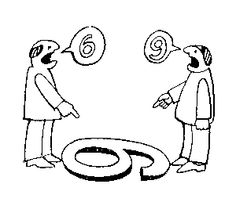
\includegraphics[width=0.49\linewidth]{./img/perceptuel.jpg} 
  \caption {Illustration du fait que deux individus peuvent avoir une interprétation divergente de l'environnement en fonction de leur situation spatiale. La capacité de comprendre que l'autre a une vision différente est liée à la prise de perspective perceptuelle (ou prise de perspective de niveau un).}
  \label{fig:perceptuel}
\end{figure}

La prise de perspective conceptuelle va plus loin et désigne la capacité d'un humain à attribuer des croyances et des sentiments aux autres\cite{Baron1985}.
Ainsi, dans l'illustration faite dans la figure \ref{fig:conceptual}, Bob fait une supposition sur l'état de croyance d'Alice concernant la contenance de la boîte.
Cette supposition que Bob fait de l'état de croyance d'Alice peut différer de l'état réel.

\begin{figure}[ht!]
 \centering
  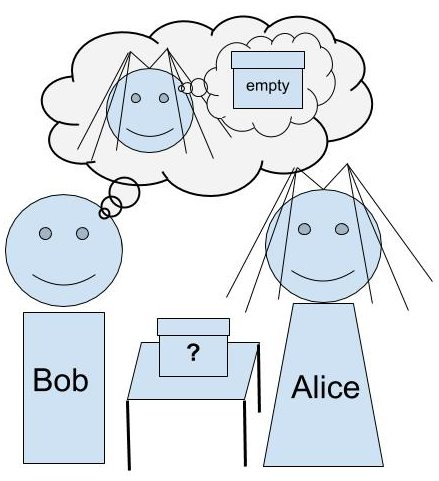
\includegraphics[width=0.49\linewidth]{./img/conceptual.jpg} 
  \caption {Illustration de la prise de perspective conceptuelle. Ici Bob attribue une croyance à Alice concernant la contenance de la boîte. Il suppose qu'elle croit que la boîte est vide. Cette faculté d'imputer des croyances aux autres s'appelle la prise de perspective conceptuelle (ou prise de perspective de niveau deux).}
  \label{fig:conceptual}
\end{figure}

Ainsi, dans la psychologie du développement, la faculté de comprendre qu'un autre puisse avoir une croyance erronée sur l'environnement qui l'entoure est considérée comme une étape importante dans l'évolution et l'acquisition de la théorie de l'esprit. Dans la littérature en psychologie, la tâche de reconnaissance de fausse croyance ("false belief task" en anglais) a été formulée dans \cite{Wimmer1983103}. Heinz Wimmer et Josef Perner définissent un test (le test de Sally et Anne) qui permet d'évaluer les aptitudes d'une personne à comprendre qu'autrui possède des états mentaux différents des siens. Le test a été par la suite réalisé par Simon Baron-Cohen et Alan M. Leslie et rapporté dans \cite{Baron1985} et une seconde version dans \cite{Leslie1988}. Ce test est expliqué dans la figure \ref{fig:sallyAndAnne}.

%TODO Put it in Annexe?
\begin{figure}[ht!]
 \centering
  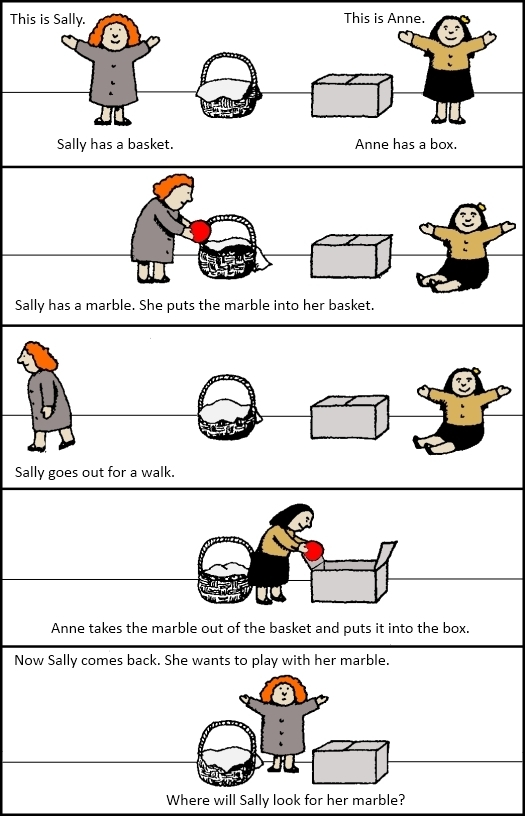
\includegraphics[width=0.89\linewidth]{./img/sally.jpg} 
  \caption {Test de Sally et Anne permettant de vérifier la capacité d'un individu à identifier un état de connaissance erroné chez autrui. Illustration basée sur l'œuvre d'Axel
Scheffler.}
  \label{fig:sallyAndAnne}
\end{figure}


%Perspective Taking is a human ability which allows one to see things from other's point of view. 
% Studied in
% psychology literature~\cite{Flavell1992,Tversky1999}, this ability is
% crucial when interacting with people by allowing one to reason on
% others' understanding of the world in terms of visual perception, spatial
% descriptions, affordances and beliefs, etc.
% Therefore, in the last years it has been gradually
% employed in Human-Robot Interaction. ~\cite{breazeal2006} presents a learning algorithm that takes into account information about a
% teacher's visual perspective in order to learn a task. ~\cite{Johnson2005} apply visual perspective taking for action
% recognition between two robots.~\cite{Trafton2005} use both visual
% and spatial perspective taking for finding out the referent
% indicated by a human partner.

% In psychology, Theory of mind (ToM) is defined as an understanding of other people’s mental states (their thoughts, feelings, desires, motivations, intentions).
% It includes perspective taking ability. Visual perspective
% taking is one of the most significant ToM precursor. 
% ToM encompasses a wide range of skills from instantaneous visual
% perspective skill to complex interpretation of other agent intents, plans,
% feelings occurring on a long time period.
% Increased ToM skills directly lead to increased performance when interacting
% with other agent in a collaborative as well as a competitive context.
% Being able to attribute false belief (to recognize that someone else
% has different beliefs about the physical world) has been considered
% as a milestone in ToM development.
% In psychology literature the false belief task was formulated in
% \cite{Wimmer1983103}.
% Breazal in ~\cite{BreazealGB09} proposed one of the first human robot
% implementation and proposed some more advanced goal recognition skills
% relying on this false belief detection.


% This paper will present an evolution of the previous work \cite{Warnier2012a} \cite{Lemaignan2012} \cite{Sisbot2011} with a refined management of divergent beliefs, temporal reasonning on data and improved inferring capabilities.
% These improvements allow the robot to pass Sally and Anne test \cite{Baron1985} (see Section IV B), to make inferences not only on position properties but also on dialogue, and other human actions.

% %%%%%%%%%%%%%%%%%%%%%%%%%%%%%%%%%%%%%

% ROMAN TOASTER 2016

\subsection{Usage en robotique}

Comme indiqué dans la partie \ref{sec:motivation}, pouvoir percevoir et raisonner sur l'environnement qui l'entoure sont des capacités nécessaires pour le robot mais non suffisantes lorsqu'il interagit avec des humains. Pour pouvoir comprendre la situation de l'humain, des recherches récentes ont tenté d'implémenter une sorte de théorie de l'esprit, en permettant au robot d'avoir la faculté de prise de perspective de niveau un (perceptuelle). Cynthia Breazeal présente dans \cite{breazeal2006} un algorithme d'apprentissage qui prend en compte l'information concernant le point de vue visuel de l'instructeur afin d'apprendre convenablement une tâche. Dans \cite{Johnson2005}, les auteurs appliquent la prise de perspective visuelle pour la reconnaissance d'action entre deux systèmes robotiques. Gregory Trafton dans \cite{Trafton2005} utilise à la fois la prise de perspective visuelle et spatiale pour identifier le référent indiqué par un partenaire humain. Dans \cite{ros2010one} la prise de perspective visuelle est utilisée pour simplifier la clarification de déclarations référentielles (referential utterances) dans des scénarios impliquant plusieurs objets.

Pour pleinement comprendre et se faire comprendre par l'homme, certaines études ont également visé à donner le niveau deux (conceptuel) de prise de perspective au robot. Cynthia Breazal dans ~\cite{BreazealGB09} propose l'une des premières implémentations faisant intervenir un humain et un robot ainsi que quelques capacités plus avancées de reconnaissance de but basées sur cette détection de fausse croyance.
%TODO Compléter la biblio sur le niveau 2
%use: http://www.csc.kth.se/~hedvig/publications/cogsci_16.pdf

%%%%%%%%%%%%%%%%%%%%%%%%%%%%%%%%%%%%%%%%%%%%%%%%%%%%%%%%%%%%%%%%%%%%%%%
% This paper will present an evolution of the previous work \cite{Warnier2012a} \cite{Lemaignan2012} \cite{Sisbot2011} with a refined management of divergent beliefs, temporal reasonning on data and improved inferring capabilities.
% These improvements allow the robot to pass Sally and Anne test \cite{Baron1985} (see Section IV B), to make inferences not only on position properties but also on dialogue, and other human actions.

%ROMAN2014
% Secondly, it must be able to gain explicit reasoning on the human it
% interacts with. It means that not only the knowledge must be
% grounded between the robot and its interactor but also that the robot
% must be able to maintain an explicit representation of the knowledge
% of its interactor apart of its own knowledge. That will allow the
% robot to compare its own beliefs with the one of the human and to
% infer similarities as well as differences and ambiguities. Thus, the
% robot must be able to handle a kind of "theory of mind" \footnote{\url{http://en.wikipedia.org/wiki/Theory\_of\_mind}}.


% Equipped with such capabilities, a robot who will interact
% with humans should be able to extract, compute or infer these
% relations and capabilities in order to communicate and interact efficiently in a natural way.

% To achieve this we identified 3 main ingredients.
% First, the consideration of perspective-taking, i.e. the ability of
% the robot not only to build a model of the world for itself but
% also to estimate what its human partners perceive.
% Secondly, the ability to compute efficiently affordances for itself
% and to estimate the affordances of its human partners in a given situation 
% Finally, the ability to
% maintain a history of beliefs based on presence and focus of attention of humans which will enable reasoning on divergent beliefs.
% We will present how these features are implemented in SPARK as a permanent activity based on inter-related processes.


%%%%%%%%%%%%%%%%%%%%%%%%
% TOASTER ROMAN2016

% To make robots more socially competent, some research aims to endow robots with this ability.
% Some robotic research use the first level to have a better understanding of the human and remove ambiguities ~\cite{Trafton2005}, ~\cite{breazeal2006}, ~\cite{ros2010one}
% %B conceptual
% Concerning level two, various research on human robot interaction already aim to represent the human belief state.
% Breazal et al.~\cite{BreazealGB09} proposed one of the first human-robot implementation. In our previous work \cite{Milliez2014}, we made a primitive implementation to solve the Sally and Anne test described by Wimmer in~\cite{Wimmer1983}. In this primitive implementation, the reasoning on others belief state was limited to object position. We propose here a more generic approach to represent any kind of belief the human may hold on the environment.



%%%%%%%%%%%%%%%%%%%%%%%%%%%%%%%%%%%%%%%%%%%%%%%%%%%%%%%%%%%%%%%%%%%%%%

\section{Prise de perspective et état mental}

\subsection{Prise de perspective perceptuelle}
\label{sec:perceptuelle}

Dans notre système, pour donner au robot la capacité de se mettre à la place de l'homme et de comprendre ce qu'il est capable de percevoir et les éléments qui sont à sa portée, nous avons ajouté le calcul de deux faits basés sur la représentation tridimensionnelle de l'état du monde expliquée au chapitre précédent. Le premier permet de connaître ce qui est visible par l'homme, c'est à dire ce qui se trouve dans son champ visuel et n'est pas caché (ou tout du moins qui est suffisamment visible).

% To estimate what is visible for a human, it computes which objects are present in a cone, emerging from human's head. 
% If the object can be directly linked to the human's head with no obstacle and if it is in the field of the view cone, 
% then we assume that the human sees the object and hence has knowledge of its position. 
% If an obstacle is occluding the object, then it won't be visible for the human. 
% Concerning the reachability, a threshold of 1 meter is used to determine if the human can reach an object or not.


Ainsi, dans la figure \ref{fig:occludedHuman}, l'humain en bleu est incapable de voir l'objet à droite (\textit{WHITE\_BOOK}) car il est caché par la boîte grise (GREY\_BOX). Le système robotique est capable, en utilisant la position de la tête de l'homme et le modèle de l'environnement, de savoir quels objets sont visibles de l'homme et quel pourcentage de l'objet est visible.
En utilisant ce pourcentage, le système peut produire un fait concernant la visibilité de l'objet avec une confiance associée. Par exemple ici, le fait serait:

\begin{scriptsize}
\begin{verbatim}

Subject   property  target    value

ROBOT     canSee  WHITE_BOOK  true
HUMAN     canSee  WHITE_BOOK  false
\end{verbatim}
%\end{small}
%\end{footnotesize}
\end{scriptsize}

%TODO: surligné l'objet occlut
\begin{figure}[ht!]
 \centering
  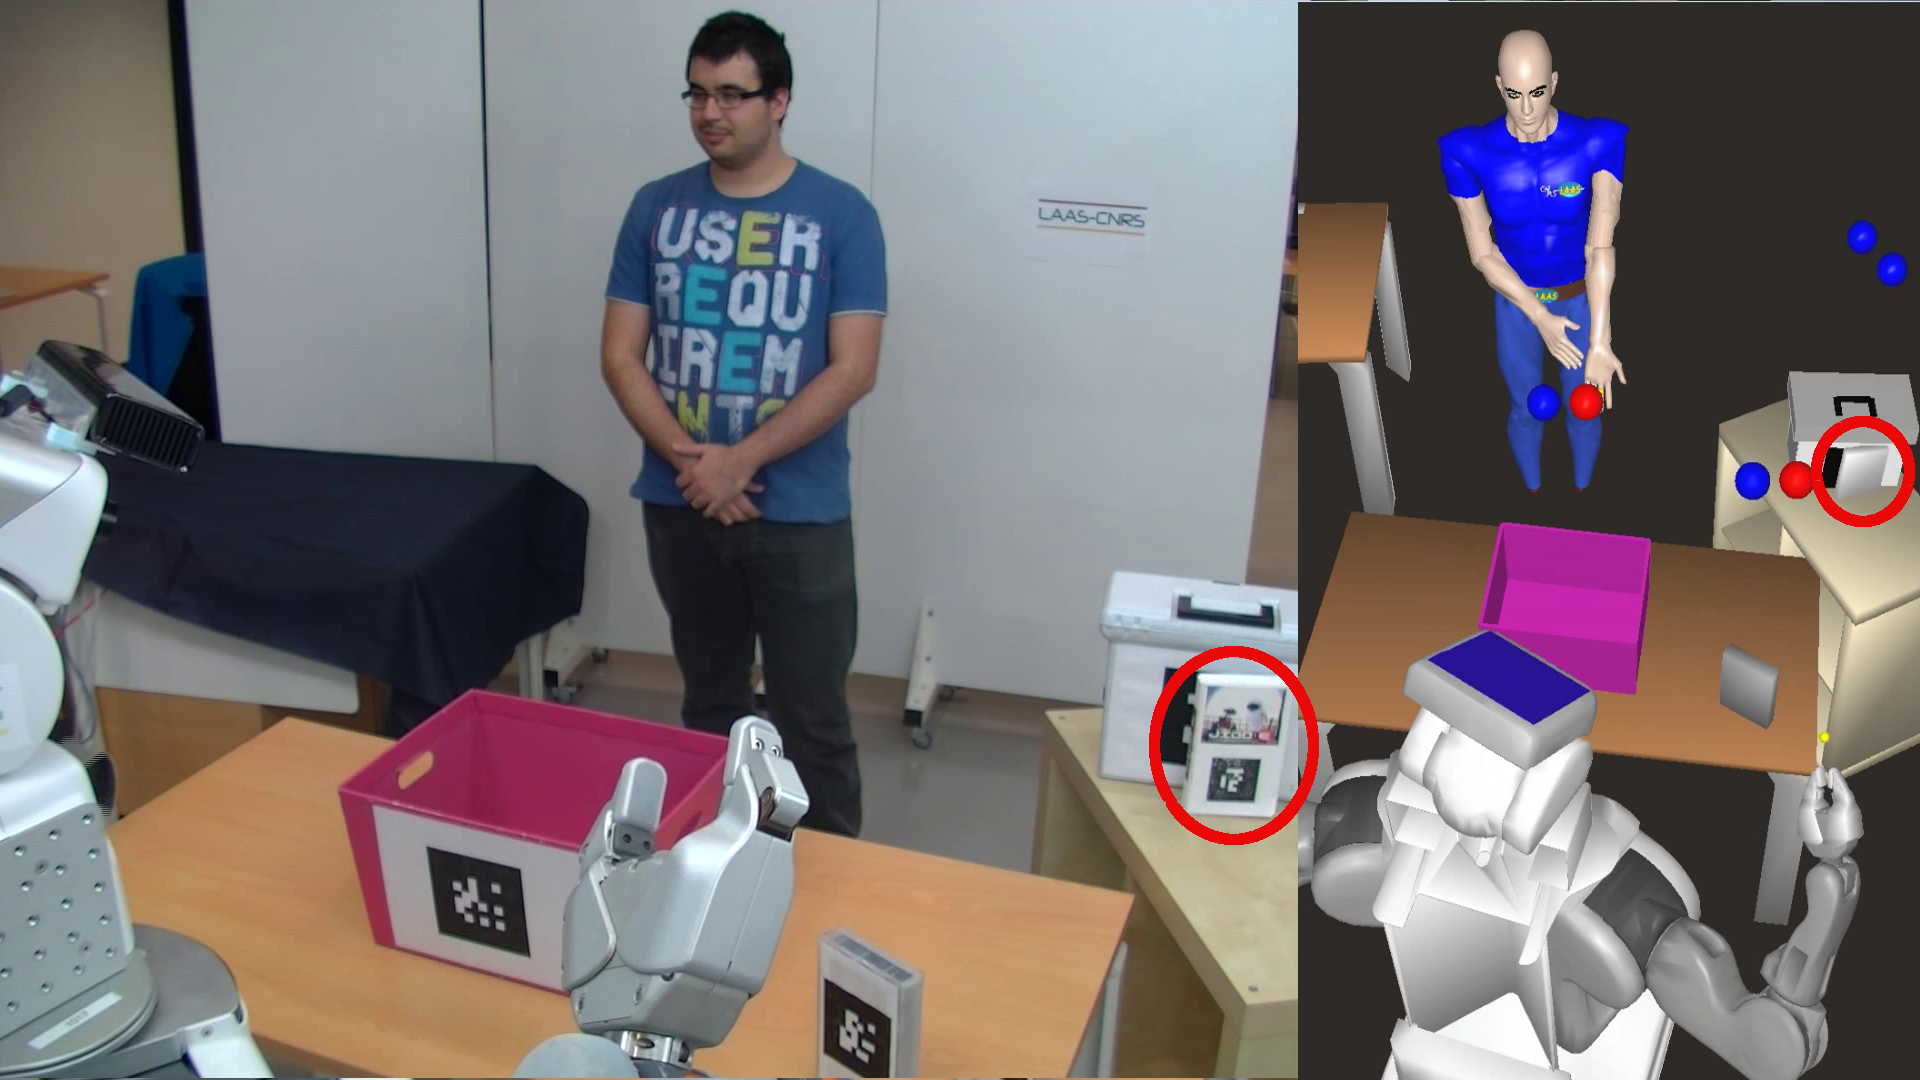
\includegraphics[width=0.99\linewidth]{./img/blueMovedPr2M.png} 
  \caption {Exemple d'état du monde où le système est capable de calculer la visibilité des objets pour chaque agent. Ici, le livre blanc n'est pas visible par l'homme.}
  \label{fig:occludedHuman}
\end{figure}


Le robot est donc capable de savoir ce qu'il est capable de percevoir (moyennant éventuellement un mouvement de tête), mais également ce que l'homme peut ou non percevoir. Nous verrons dans le chapitre suivant comment cela peut être utilisé durant une interaction, notamment pour améliorer le dialogue situé en terme d'efficacité.

Le second fait ajouté concerne le calcul permettant de savoir si les objets qui entourent l'homme sont à sa portée. En utilisant la bibliothèque 3D Move3D  \cite{Simeon2001}, il est en effet possible de calculer la cinématique inverse d'un agent et de planifier ses mouvements. Grâce à cela, il est donc possible de savoir quels objets sont accessibles aux agents de la scène en prenant en compte les collisions éventuelles comme expliqué dans \cite{sisbot2011situation}. Ce calcul est illustré par l'image \ref{fig:reach}, où le robot calcule l'accessibilité d'un objet par rapport à lui-même et à l'homme présent dans la scène.



\begin{figure}[ht!]
 \centering
  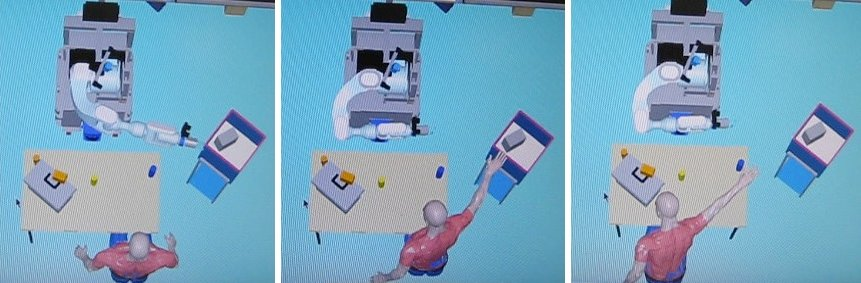
\includegraphics[width=0.99\linewidth]{./img/reach.jpg} 
  \caption {Exemple d'état du monde où le système calcule si les agents sont capables d'atteindre un objet. Sur l'image de gauche, le robot est capable de calculer qu'il peut attraper l'objet gris. Il calcule également que l'homme peut attraper l'objet gris, comme illustré par l'image centrale. Si l'homme avait été placé plus loin, le robot aurait pu calculer que l'objet était inaccessible pour l'homme, comme illustré par l'image de droite.}
  \label{fig:reach}
\end{figure}


La liste des faits (simplifiés) produits pour cette scène concernant l'accessibilité de l'objet gris serait pour les différentes configurations:

\begin{scriptsize}
\begin{verbatim}
left and center pictures                   right picture

Subject   property  target    value        Subject   property  target    value

ROBOT     canReach  GREY_OBJ  true         ROBOT     canReach  GREY_OBJ  true
HUMAN     canReach  GREY_OBJ  true         HUMAN     canReach  GREY_OBJ  false
\end{verbatim}
%\end{small}
%\end{footnotesize}
\end{scriptsize}

Pouvoir connaître quels objets sont à la portée de l'homme permet au robot de produire des plans collaboratifs prenant en compte cette donnée pour l'allocation de tâche, comme dans \cite{gharbi2015}.
Par exemple, si la tâche collaborative est de ranger des livres dans une boîte, si on a les faits:

\begin{scriptsize}
\begin{verbatim}

Subject   property  target     value

ROBOT     canReach  BLUE_BOOK   true
ROBOT     canReach  WHITE_BOOK  false
ROBOT     canReach  BASKET      false
HUMAN     canReach  BLUE_BOOK   false
HUMAN     canReach  WHITE_BOOK  true
HUMAN     canReach  BASKET      true
\end{verbatim}
%\end{small}
%\end{footnotesize}
\end{scriptsize}

le plan créé prendra en compte que le livre bleu (BLUE\_BOOK) et le panier (BASKET) sont atteignables par le robot pour lui assigner la tâche de ranger ce livre. De même, comme le livre blanc (WHITE\_BOOK) et le panier sont atteignables par l'homme, la tâche de le ranger lui sera assignée.
Ce fait peut également aider à lever l'ambiguïté, par exemple si l'homme demande au robot d'apporter un objet, il est peu probable que l'homme face référence à un objet qui est à sa portée.

%mais également comprendre la situation de l'homme avec lequel il intéragit.
Pour comprendre l'homme, il est également important de comprendre sa situation spatiale, à savoir comment celui-ci est entouré et comment il est susceptible de décrire ce qui l'entoure par rapport à sa position.

Nous avons donc ajouté dans notre système d'évaluation de la situation la possibilité de faire des requêtes pour obtenir la position d'une entité du point de vue d'un agent. Il est par exemple possible de calculer de quel côté une entité se trouve (gauche, droite, avant, arrière).
De plus, il est aussi possible d'obtenir la position d'une entité comparativement à une autre du point de vue d'un agent. Par exemple, il est possible pour le robot de dire à l'homme "la tasse que vous cherchez est \textbf{à votre droite}" ou "Donnez moi le livre qui est \textbf{pour vous à gauche de la tasse rouge}".
Ces requêtes permettent donc au robot d'avoir une prise de perspective géométrique et ainsi de parler à l'homme en prenant son propre référentiel, améliorant ainsi les performances sociales du robot.

\begin{figure}[ht!]
 \centering
  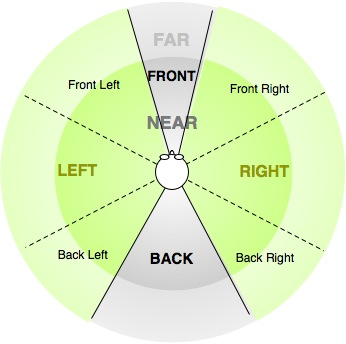
\includegraphics[width=0.59\linewidth]{./img/relative_position.jpg} 
  \caption {Illustration du découpage géométrique pour désigner les emplacements en prenant l'homme comme référentiel. Cette illustration provient de la documentation de SPARK: \url{https://www.openrobots.org/wiki/spark/what_spark_computes}.}
  \label{fig:relativePose}
\end{figure}


\subsection{Prise de perspective conceptuelle}
\label{sec:beliefm}
\subsubsection{Modélisation des états mentaux}
Nous avons expliqué dans le chapitre \ref{chapter1} qu'il est important de faire des hypothèses sur la position des objets pour pouvoir en assurer le suivi. Bien que nécessaire, le fait de créer des hypothèses implique la possibilité de se tromper.
%En conclusion du chapitre 2, nous avons expliqué comment il est possible de probabiliser l'état du monde pour prendre en compte l'incertitude du robot.
Dans cette section nous allons expliquer comment la prise de perspective va permettre au robot d'avoir connaissance de l'état de croyances des hommes avec lesquels il interagit et ainsi savoir lorsqu'ils ont une croyance erronée concernant l'environnement.

La première étape pour pouvoir connaître l'état mental d'un humain est d'avoir connaissance des informations qu'il reçoit. L'humain peut recevoir des informations sur son environnement de deux façons: soit il les reçoit directement (ou les déduit) de ses capacités perceptives, soit il les reçoit d'un autre agent à travers le dialogue.
Pour donner au robot la capacité de prise de perspective décrite en \ref{sec:psy}, nous nous focalisons dans un premier temps sur la perception et sur le dialogue homme-robot pour déduire quelles informations l'humain peut acquérir.

Grâce aux calculs des affordances des agents expliqués en \ref{sec:perceptuelle}, il est possible de savoir lorsqu'un agent perçoit un objet. Lorsqu'un humain voit un objet, cela implique qu'il acquiert la connaissance de sa localisation, et donc met à jour cette information dans son état mental. Cela permet donc de suivre l'état de connaissance de chaque agent.

L'état mental de chaque agent (tel qu'il est estimé par le robot) est ainsi conservé et mis à jour dans un modèle séparé de l'état de connaissance que le robot lui-même possède sur l'environnement. Ainsi, le modèle représentant l'état mental de chaque agent se traduit par une liste de faits. Chaque modèle est indépendant et cohérent d'un point de vue logique.

%TODO speak about database implementation?

% In SPARK we have the position of humans (see III 1.). We use it to
% calculate affordances of each human toward elements of the scene he can interact with.
% To estimate what is visible for a human, it computes which objects are present in a cone, emerging from human's head. 
% If the object can be directly linked to the human's head with no obstacle and if it is in the field of the view cone, 
% then we assume that the human sees the object and hence has knowledge of its position. 
% If an obstacle is occluding the object, then it won't be visible for the human. 
% Concerning the reachability, a threshold of 1 meter is used to determine if the human can reach an object or not.

%comment peut etre mettre un exemple de modèle d'agent,
%  même tout petit pour mettre les idées en place ?}


\subsubsection{Gestion de croyances divergentes}
\label{sec:divB}
Dans certains cas, l'homme et le robot peuvent avoir un modèle qui contient des valeurs différentes. Cela peut provenir d'une vision différente de la scène (e.g. certaines propriétés sont accessibles uniquement au robot, donc l'homme n'en a pas connaissance).
Cela peut provenir de croyances divergentes entre l'homme et le robot (e.g. l'homme croit qu'un objet a la propriété \textit{P} alors que le robot sait que cette propriété est fausse). Dans ce second cas, la prise de perspective n'est pas suffisante pour comprendre la croyance erronée de l'homme. Il est nécessaire de mettre en place la gestion de croyance divergente (divergent belief management en Anglais).


% This Management relies on data from the environment as well as from
% affordances and supervisor.
% This way, the robot can generate beliefs according to the task stated in correlation with  affordances 
% as shown in fig. ~\ref{beliefs_fg}.

% \begin{figure}[ht!]
%  \centering
%   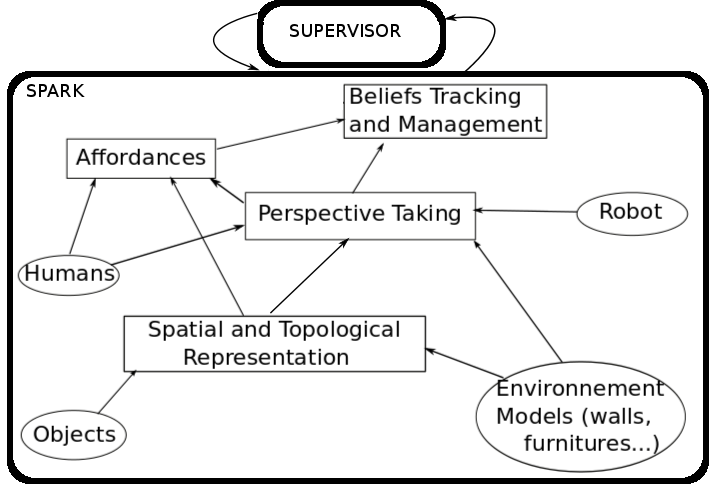
\includegraphics[width=0.99\linewidth]{./img/beliefs2.png} 
%   \caption {Schema of SPARK reasoning to generate beliefs}
%   \label{beliefs_fg}
% \end{figure}

Ici, nous traitons uniquement de propriétés n'ayant pas d'évolution prédictibile. En effet, certaines propriétés ont une évolution prédictible, comme la température d'un breuvage, la fraîcheur d'une peinture... Ceci signifie que la propriété évolue et que cette évolution peut-être estimée sans observation. Par exemple, si un humain sait qu'une tasse de thé est chaude, en revenant une heure plus tard, sans avoir à observer la tasse, il va pouvoir estimer qu'elle est froide.
Pour simplifier, nous considérons donc uniquement les propriétés dont l'évolution ne peut être prédite, comme c'est souvent le cas lorsqu'un autre agent agit sur l'environnement et modifie l'état d'une propriété (déplacement d'objet, remplir ou vider un container...).

Par exemple, si on considère qu'un humain appelé \textit{GREG} quitte la zone d'interaction avec la croyance qu'un objet \textit{Obj} a la propriété \textit{Prop} dans un état \textit{e1}.

On présente ci-dessous l'état de connaissance du robot et celui de \textit{GREG} tel qu'il est modélisé par le robot.

\begin{scriptsize}
\begin{verbatim}
          ROBOT                  GREG
      Obj Prop e1            Obj Prop e1
\end{verbatim}
%\end{small}
%\end{footnotesize}
\end{scriptsize}

Durant son absence, imaginons que la propriété \textit{Prop} appliquée à \textit{Obj} a évolué pour atteindre un état \textit{e2}.
Lorsque \textit{GREG} revient, même si la propriété a évolué, il pensera probablement que la propriété est dans le même état que lorsqu'il a quitté la scène, jusqu'à ce qu'il soit capable de réévaluer ses croyances en utilisant le dialogue ou la perception. Pour prendre en compte ce type de situation, le robot garde inchangé le modèle d'un agent lorsque celui-ci n'est pas présent pour observer les actions ou constater les changements induits, et ce jusqu'à son retour.

Avant que l'homme ne revienne, la croyance du robot a donc évolué mais pas celle de l'homme.

\begin{scriptsize}
\begin{verbatim}
          ROBOT                  GREG
      Obj Prop e2            Obj Prop e1
\end{verbatim}
%\end{small}
%\end{footnotesize}
\end{scriptsize}

Lorsque l'homme revient, on identifie trois situations différentes:

%%%%%%%%%%%%%%%%%%%%%%%%%%%%%%%%%%%%%%%%%%%%%%%%%%%%%%%%%%%%%%%%%%%
%illustrate each situation with images
\begin{itemize}
\item Dans le premier cas, l'homme remarque le changement d'état de la propriété et corrige directement sa croyance erronée. Le robot corrige donc automatiquement le vecteur de faits représentant les croyances de \textit{GREG} avec le nouvel état de la propriété. 

%illustrate each situation with images

\begin{scriptsize}
\begin{verbatim}
          ROBOT                  GREG
      Obj Prop e2            Obj Prop e2
\end{verbatim}
%\end{small}
%\end{footnotesize}
\end{scriptsize}


Pour illustrer, on peut prendre comme objet une radio (\textit{RADIO}) et comme propriété l'état (\textit{turnedOn}) qui peut avoir comme valeur allumée (\textit{TRUE}) ou éteinte (\textit{FALSE}). Si \textit{GREG} quitte la scène en sachant que la radio est allumée, lorsqu'il revient, n'entendant plus la radio, il pourra directement déduire la nouvelle valeur de la propriété d'état liée à la radio (éteinte).

%illustrate each situation with images

\begin{scriptsize}
\begin{verbatim}
          ROBOT                  GREG
    RADIO turnedOn FALSE   RADIO turnedOn FALSE
\end{verbatim}
%\end{small}
%\end{footnotesize}
\end{scriptsize}


\item Dans le second cas, l'homme remarque le changement mais est dans l'incapacité de connaître le nouvel état de la propriété. L'humain étant au courant de son ignorance, le robot supprime sa croyance erronée. Pour ce faire, il met à jour le vecteur de faits avec un état \textit{unknown} qui traduit le fait que le robot ait connaissance que l'homme sait qu'il ignore le nouvel état de la propriété.


\begin{scriptsize}
\begin{verbatim}
          ROBOT                  GREG
      Obj Prop e2            Obj Prop unknown
\end{verbatim}
%\end{small}
%\end{footnotesize}
\end{scriptsize}



On peut prendre cette fois comme exemple un livre (\textit{BOOK}) ayant comme propriété une position (\textit{isOn}) et pouvant avoir pour valeur le meuble sur lequel il se trouve (\textit{LIVINGROOM\_TABLE}, \textit{BEDSIDE\_TABLE}, \textit{BEDROOM\_SHELF}). Si \textit{GREG} quitte la scène en sachant que le livre est sur la table du salon, lorsqu'il revient, s'il observe que le livre n'est plus à sa place, il aura alors connaissance que la propriété de position a changé de valeur sans être capable de savoir la nouvelle valeur de celle-ci tant qu'il n'aura pas vu l'objet.

\begin{scriptsize}
\begin{verbatim}
          ROBOT                         GREG
     BOOK isOn LIVINGROOM_TABLE    BOOK isOn unknown
\end{verbatim}
%\end{small}
%\end{footnotesize}
\end{scriptsize}



\item Dans le troisième cas, l'homme est incapable de remarquer que la propriété a changé. L'humain va alors garder sa croyance erronée concernant la propriété jusqu'à ce qu'il puisse constater un changement ou que le robot l'informe de l'évolution de la propriété. 

\begin{scriptsize}
\begin{verbatim}
          ROBOT                  GREG
      Obj Prop e2            Obj Prop e1
\end{verbatim}
%\end{small}
%\end{footnotesize}
\end{scriptsize}

Pour prendre un dernier exemple, si l'objet est une boîte de cookies (\textit{COOKIE\_BOX}) opaque et que la propriété décrit la présence de cookies à l'intérieur de la boîte (\textit{isFull}), pouvant prendre pour valeur pleine (\textit{TRUE}) ou vide (\textit{FALSE}). Si lorsque \textit{GREG} quitte la scène il pense que la boîte est vide, si celle-ci a été remplie pendant son absence, \textit{GREG} sera incapable de savoir que la boîte est à présent remplie tant que celle-ci sera fermée (et donc l'état de la propriété \textit{isFull} non observable).

\begin{scriptsize}
\begin{verbatim}
           ROBOT                         GREG
COOKIE_BOX isFULL TRUE        COOKIE_BOX isFULL FALSE
\end{verbatim}
%\end{small}
%\end{footnotesize}
\end{scriptsize}
\end{itemize}

Pour résumer et formaliser ces différentes situations pour la mise à jour de l'état mental d'un autre agent, nous notons:

\begin{itemize}
\item \textit{HB} le modèle de croyance de l'humain \textit{H} et \textit{RB} celui du robot \textit{R}.
\item \textit{p} représente une propriété de l'environnement.
\item \textit{value(p,m)} représente la valeur de la propriété \textit{p} dans le modèle \textit{m}.
\item \textit{evo(p,A)} représente la capacité de l'agent \textit{A} à percevoir l'évolution de la propriété \textit{p}. \textit{evo(p,A)} peut prendre les valeurs \textit{UNSEEN} lorsque l'agent n'est pas au courant de l'évolution, \textit{INVALIDATE} lorsqu'il sait que la propriété a évolué sans connaître la nouvelle valeur et \textit{UPDATE} lorsqu'il est capable d'observer ou estimer la nouvelle valeur.
\end{itemize}

Dans le cas où il y a une croyance divergente, c'est à dire: \newline
if $p\in RB,\quad p\in HB \land value(p,HB)\neq value(p,RB)$

On a alors les trois situations précédentes qui peuvent être représentées par les règles:

\begin{itemize}
\item if $evo(p,HB)=UNSEEN  \rightarrow value(p,HB) = value(p,HB)$
\item if $evo(p,HB)=INVALIDATE  \rightarrow value(p,HB) =\textit{unknown}$
\item if $evo(p,HB)=UPDATE  \rightarrow value(p,HB) = value(p,RB)$
\end{itemize}

Il est alors à constater que la partie complexe pour mettre à jour correctement les croyances de l'homme est de modéliser convenablement sa capacité à percevoir l'évolution de la propriété et donc l'obtention de la valeur de \textit{evo(p,HB)}. Dans la section suivante nous présentons notre implémentation pour l'état de croyance des agents et nous proposons une solution pour l'estimation de cette valeur.
%%%%%%%%%%%%%%%%%%%%%%%%%%%%%%%%%%%%%%%%%%%%%%%%





% Knowing these beliefs is a great help to the robot to understand human and interact with him.
% The robot takes human's perception into account to have appropriate interpretation of human requests, to proactively inform or warn the human about a missing or wrong belief and also to generate a collaborative plan. 
% Thus, the robot has to reason on what a human can see, reach and
% knows to get these skills.




%%%%%%%%%%%%%%%%%%%%%%%%%%%%%%%%%%%%%%
% ROMAN2016 INTENTION
% We consider our world as a dynamic environment, where entities can move, objects' properties can change and actions can be performed.  We define an action as a tuple $(name, preconditions, target, postconditions)$. The $name$ of an action is a unique string that identifies it. The $preconditions$ are a list of properties that must be true in order to realize the action. In our system, an action is executed on a $target$, which can be a physical object, like a cup, but also an area of the environment, like a room. The $postconditions$ are the set of properties, and their values, affected by the action's execution.

% Since we are interested, in this paper, on reasoning and not perceptual aspects, we use inference, as explained in Sec. \ref{sec:intention_recognition}, in order to understand when a human has performed an action. Through the predefined $postconditions$ of actions we can also infer changes in object properties, e.g. the human opens a box, so the box is now open. 

% Since the environment is dynamic, agents can have divergent representations of the world. To model this aspect, the information produced by perception, geometrical reasoning and inference, are collected by the robot in \textit{belief models}, built for itself and for each agent. A \textit{belief model} is a symbolic representation of the world state, as known by an agent. In a model, the world state is represented by properties and values. To represent the lack of knowledge of an agent, the value of a property can be \textit{unknown}.
% We created a rule based framework in order to build beliefs of each agent and update them when needed. Human belief models are updated using the perspective taking skills of the robot. When the robot detects the execution of an action in the world, it updates the belief model for itself and for every human that can perceive the action, adding the action's $postconditions$ to their models. When an action is not perceived by a human (e.g. the user was in an other room), his belief model won't be updated, as he is not aware of the changes that occurred.



\section{Implémentation}
%BASE DE DONNÉE
%(Implémentation)

\subsection{Traitement générique de la mise à jour de l'état de croyance}
\label{sec:dbPt}
Pour pouvoir avoir un état du monde symbolique pour chaque agent afin de représenter la conception mentale que celui-ci a de l'environnement, il est possible d'ajouter des tables dans la base de données temporelle.
Chaque table est comparable à la table \textit{ROBOT\_WS\_TBL} décrite en section \ref{sec:dbd} et qui contient une liste de faits décrivant l'état du monde perçu par le robot lui-même.
En plus de ces tables contenant la représentation symbolique de l'environnement du point de vue d'un agent tel qu'elle est estimée par le robot, nous ajoutons également une table mémoire pour chaque agent. Cette table représente l'état de croyance passée de l'agent courant. Elle est comparable à la table \textit{ROBOT\_MEM\_TBL} décrite en section \ref{sec:dbt}.

Cependant, pour le robot la mise à jour de ces tables repose directement sur la perception de l'environnement basée sur les différents modules de TOASTER décrits en section \ref{sec:calculs} et sur le module de gestion des hypothèses décrit en section \ref{sec:hypo}. Pour pouvoir mettre à jour les croyances de l'homme, il faut pouvoir mettre en place une gestion des croyances telle que décrite en section \ref{sec:divB}.

Pour ce faire, comme expliqué en section \ref{sec:divB}, lorsqu'un agent ne peut percevoir un événement, son état mental reste inchangé.
Toute la difficulté ici est de parvenir à estimer lorsque l'homme est capable ou non de mettre à jour son état de croyance (c'est à dire la valeur de \textit{evo(p,HB)} décrit dans \ref{sec:divB}).
En effet, selon la propriété concernée, l'état peut être plus ou moins observable ou déductible selon divers moyens de perception.

Par exemple, la propriété de localisation d'un objet est une propriété directement observable lorsque l'objet est visible. En effet, si un homme observe un objet, il aura directement la connaissance de sa position. Par contre, si l'on reprend l'exemple de la boîte de cookies, l'observabilité de la propriété de contenance dépend de la propriété relative à l'ouverture de cette boîte. Ainsi, il est possible d'observer la contenance de la boîte de cookie seulement si celle-ci est ouverte.
De plus, la perception peut passer par diverses modalités. Par exemple pour savoir qu'une tasse est chaude il est possible, soit de percevoir de la fumée émanant de la tasse, soit de ressentir la chaleur de celle-ci dans la main.
Enfin, l'observabilité est également liée aux capacités de perception de chaque agent. Ainsi, si l'on reprend le cas de la radio, une personne sourde ne sera pas en capacité de savoir si celle-ci est allumée ou éteinte.

Afin de proposer une première implémentation et de mettre en place une gestion générique des hypothèses et du maintien de l'état mental de chaque agent, nous avons ajouté à chaque fait une notion d'observabilité, correspondant au champ \textit{factObservability} déjà présenté en section \ref{sec:facts} lors de la présentation de la structure de \textit{fait}.
L'observabilité représente la probabilité qu'un agent puisse acquérir l'état d'une propriété lorsque le sujet (\textit{subject}) du fait est visible.

Pour gérer la mise à jour, nous utilisons les règles suivantes qui sont une adaptation des règles énoncées en section \ref{sec:divB}. Nous rappelons les notations précédemment utilisées et en introduisons de nouvelles.

\begin{itemize}
\item \textit{HB} le modèle de croyance de l'humain \textit{H} et \textit{RB} celui du robot \textit{R}.
\item \textit{p} représente une propriété de l'environnement.
\item \textit{value(p,m)} représente la valeur de la propriété \textit{p} dans le modèle \textit{m}.
\item \textit{obs(p)} signifie que la propriété \textit{p} est observable.
\item \textit{probObs(p)} est l'observabilité de la propriété comme définie précédemment.
\item \textit{valid(p,A)} signifie que la propriété \textit{p} ne contredit pas la perception courante de l'agent \textit{A}.
\item \textit{vis(p,A)} signifie que l'agent \textit{A} est capable de voir (lié à la propriété \textit{canSee} évoqué en section \ref{sec:perceptuelle}) l'entité sujet de la propriété \textit{p}.
\item \textit{conf(p,A)} représente la confiance que le robot a dans le fait que l'agent \textit{A} ait effectivement mis à jour la valeur de la propriété \textit{p}.
\end{itemize}

L'évaluation de la validité d'une propriété étant hautement variable, il n'a été implémenté pour l'instant que pour les propriétés de position. En effet, pour les propriétés de position, le fait de pouvoir observer l'emplacement précédent suffit à savoir que la propriété n'est plus valide.
Nous avons donc l'ensemble des règles de mise à jour suivant, pour chaque propriété  $p\in HB \cup RB$: 



% We call $H$ the agent, $HB$ his belief model, and $RB$ the robot's belief model. We also create the following predicates: $obs(p)$ means that the instance of property $p$ is observable, $valid(p,x)$ means that the instance of property $p$ doesn't contradict the current perception data of agent $x$, $value(p,m)$ is the value of predicate $p$ in belief model $m$, and $vis(p,x)$ means that agent $x$ has visibility on the linked entities of property $p$. The rules for the $valid$ predicate will be different in each property. For example the property \textit{MUG isOn TABLE} won't be valid for agent Max if he can see that there is no mug on the table. For each property $p\in HB \cup RB$:
\begin{itemize}
\item if $p \in RB, \quad p\not\in HB,\quad obs(p),\quad vis(p,H) \rightarrow value(p,HB)=value(p,RB)$.
\item if $p \not \in RB,\quad p\in HB,\quad obs(p),\quad vis(p,H) \rightarrow remove\quad $p$ \quad from \quad HB$.
\item if $p\in RB,\quad p\in HB$ then:
	\begin{itemize}
      \item if $value(p,HB)\neq value(p,RB),\\ \quad obs(p),\quad vis(p,H) \rightarrow  value(p,HB)=value(p,RB)$ \\
      $conf(p,H)=vis(p,H)*probObs(p)$.
      \item if $value(p,HB)\neq value(p,RB),\\ \quad !obs(p),\quad !valid(p,H) \rightarrow  value(p,HB)=\textit{unknown}$.
	\end{itemize}
\end{itemize}

L'idée de cet ensemble de règles est de mettre à jour le modèle d'état mental d'un agent \textit{A} seulement si le sujet de la propriété (pouvant être n'importe quel entité à savoir un homme, un robot, un objet ou le membre d'un agent) est observable par \textit{A}, ou, dans le cas d'invalidité, s'il n'est pas observable mais que les données de perception contredisent la valeur actuelle de la propriété. Par exemple si une tasse a été déplacée de la table de la cuisine à une étagère, en l'absence de \textit{A}, même si \textit{A} ne peut voir où est la tasse, il peut voir qu'elle n'est plus sur la table.


\subsection{Réflexion sur d'éventuelles améliorations}
La méthode d'implémentation, basée sur les règles définies ci-dessus, permet un traitement "automatique" et générique des diverses propriétés.
Cependant, cette implémentation est simplifiée car, comme indiqué précédemment, 
l'observation de l'invalidité d'une propriété ou l'acquisition du nouvel état d'une propriété peut être très variable d'une propriété à l'autre.

L'une des façons d'améliorer simplement les règles déjà existantes serait de considérer l'observabilité d'une propriété non seulement en la basant sur la visibilité du sujet de la propriété par l'agent concerné, mais aussi de la cible pour certaines propriétés telles que les propriétés de relations entre objets (isOn, isIn, isNextTo) ou de capacités des agents (canReach, canSee). Ainsi selon la propriété, la mise à jour de l'état pourrait être liée à la possibilité de voir le sujet ou la possibilité de voir la cible ou la possibilité de voir les deux à la fois.

Une autre façon d'améliorer la gestion des croyances serait de créer un ensemble de règles définissant les différents moyens de mise à jour d'une propriété.
Ainsi, pour le problème de la propriété de contenance de la boîte opaque, il faudrait vérifier que: la boîte est visible par l'agent, que son contenu est visible et que la boîte est ouverte.
Un autre exemple, pour savoir qu'un agent \textit{H1} est capable de savoir qu'un agent \textit{R} peut voir un objet \textit{O} il lui faut non seulement pouvoir voir la position de \textit{R} mais aussi connaître (ou voir) la position de l'objet \textit{O}.
Cette méthode, bien qu'envisageable, nécessiterait de définir des règles pour chaque propriété, ou tout du moins chaque type de propriétés, et donc nécessite de définir un domaine réduit avec des règles données au robot par un expert.
Un moyen d'éviter cela serait de développer des mécanismes d'apprentissage afin que le robot puisse produire lui-même ces règles.


%TODO finir: expliquer comment ça marche, ajouter des formules?
%observabilité subject / target?

%we assumed in previous chapter that perception object update property.
%However, for some properties visual, some different...
% We assume here that if the human is able to perceive an object property, he is then aware of the object property state. As an example for position property, if there is no obstacle between his eyes and the object and the object is in the human field of view, 
% he is then aware of its position.

%explain how we do -> observability
%explain that it is a first approximation, hypothesis are based on lot of things.
%confidence should shrink with time
%Database, cf roman 2016

%TODO: then detail how to update mental states: different for position hypothesis (sub symbolic) and other properties. observability Or maybe put it in implementation?
%Visual pereception -> position, light on...
%Some are not easily perceived by vision: hot, isFull...

\section{Résultats expérimentaux}
%Sally and Anne + experience améliorée, cf Roman 2014

%%%%%%%%%%%%%%%%%%%%%%%%%%%%%%%%%%%%%%%%%%%%%%%%%%%%%%%%%%%%%%%
Nous présentons ici l'une des expériences menées au LAAS permettant de mettre en valeur la capacité du système à maintenir et mettre à jour l'état mental des humains présents grâce aux mécanismes de suivi et de mise à jour d'état mental présentés précédemment.

\subsection{Configuration expérimentale}
\label{sec:chap2expconf}
Tout d'abord, nous présentons brièvement les capteurs et modules que nous utilisons pour les expérimentations.


Ces expérimentations ayant été réalisées en 2014, l'infrastructure logicielle utilisée pour l'estimation de la situation est SPARK\cite{sisbot2011situation,warnier2012when,Milliez2014}, qui est une version antérieure à TOASTER mais qui a un fonctionnement similaire pour le suivi de l'état mental des humains concernant les propriétés de position des objets.

%TODO: redo
\begin{figure}[ht!]
  \centering
  %% \includegraphics[width=0.7\textwidth]{./figs/supervisor-architecture-new.pdf} \\
% \includegraphics[width=0.5\textwidth]{./image/sparkinput.png} \\
 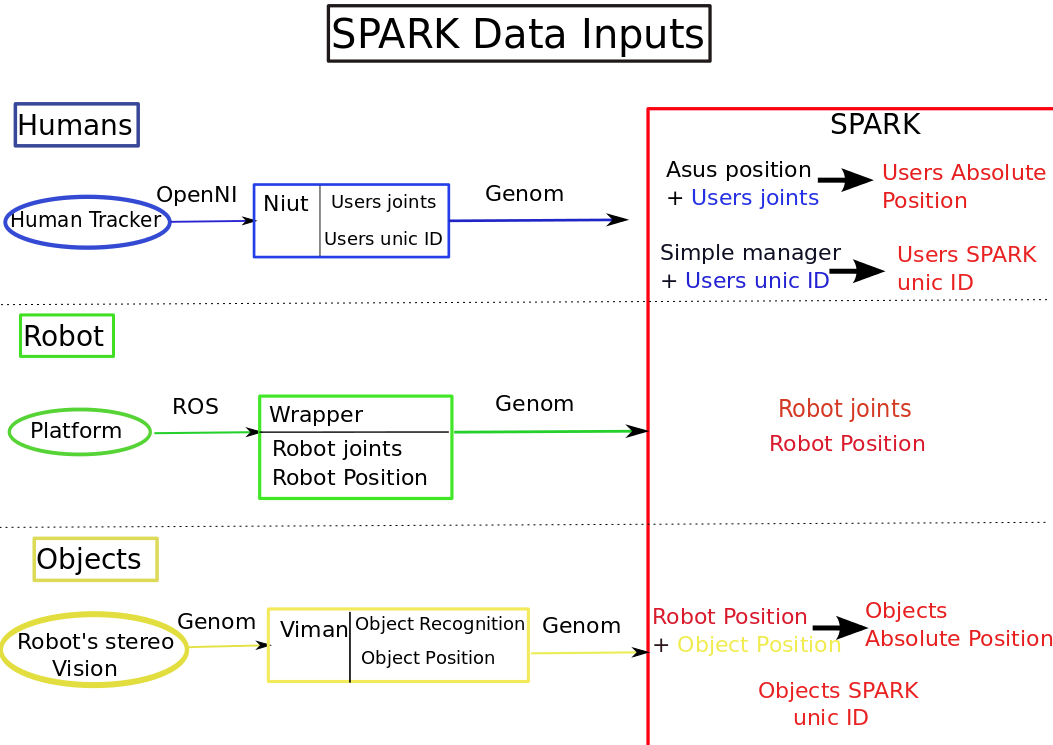
\includegraphics[width=0.99\linewidth]{./img/spark_input.png} 
  \caption {Schéma représentant les entrées de SPARK.}
  \label{fig:inputSpark}
\end{figure}

Pour assurer le suivi des humains, nous utilisons une Asus xtion \footnote{\url{https://www.asus.com/fr/3D-Sensor/Xtion_PRO}}. Comme le fait de bouger la tête est une partie importante de la communication pour permettre au robot de montrer son attention, et pour éviter la perte du suivi, nous avons fixé l'Asus xtion sur une base stable derrière le robot.
Un module, appelé \textit{niut}, est responsable de la gestion du suivi des humains, en utilisant l'API OpenNI. Ce module fait également une identification des humains basée sur la teinte. Pour obtenir la valeur moyenne de la teinte de chaque humain, on extrait la position du torse, puis nous la projetons dans les coordonnées de l'image RGB. Si les données sont disponibles, le module utilise également les coordonnées des épaules et des hanches pour définir le rectangle dans lequel la teinte sera calculée, sinon le module crée un rectangle autour de la position du torse, en adaptant l'échelle en fonction de l'éloignement de l'humain.
En donnant au module les valeurs des teintes de chaque humain, il est possible de reconnaître l'humain et d'envoyer ses données de posture au module d'estimation de la situation avec un id unique. Cela permet également de filtrer les faux positifs dans la détection d'humains et évite que des humains non enregistrés perturbent le déroulement des expériences.
Pour que les hommes soient à la bonne position dans le modèle du monde, une projection est effectuée à partir de la position et l'orientation de l'Asus xtion.

La posture et la position du robot sont directement obtenues grâce à ses capteurs internes en utilisant l'intergiciel ROS.

Enfin, pour obtenir la position des objets, nous utilisons le module \textit{Viman} qui est basé sur la bibliothèque de réalité augmentée ARToolKit\footnote{http://artoolkit.org/}. Ce module utilise la vision stéréo du robot pour reconnaître et localiser les objets. Pour ce faire, \textit{viman} scanne des RTags placés sur les objets.
Une fois que la position relative (à la caméra) de l'objet est connue, elle est envoyée au module d'estimation de la situation qui, en utilisant la position de la tête du robot pourra obtenir la position de l'objet dans le monde par projection.
La figure \ref{fig:inputSpark} illustre cette implémentation.


\subsection{Résultats}
\label{sec:ResChap2}


Nous avons introduit ci-dessus comment nous procédons pour suivre les croyances distinctes pour chaque agent. Nous croyons que cette fonctionnalité est utile pour comprendre la verbalisation de l'homme, ses actions et la focalisation de son attention, i.e. pour interagir avec des humains. Comme le robot connaît les croyances des humains, il peut décider des informations qui sont nécessaires à fournir à l'homme et également s'il doit parler ou non en fonction de la situation actuelle ou de l'état de réalisation du plan collaboratif. La fonctionnalité de gestion de croyance présentée dans ce chapitre a été utilisée sur un robot afin de la tester \footnote{Des vidéos des expérimentations sont accessibles à l'url: \url{http://homepages.laas.fr/gmilliez/roman2014/}}.




\subsubsection{Le Test de Sally et Anne}

Pour aider à la compréhension des scénarios, la figure \ref{SA} et la figure  \ref{divB} sont des images de l'expérimentation réelle avec des captures d'écran de la modélisation 3D du module de raisonnement spatial.


\begin{figure*}[ht!]
  \begin{center}
    \subfigure[Greg (en vert) et Bob (en bleu) font face au robot. Ils connaissent la position de chaque objet.]{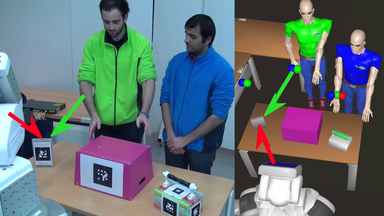
\includegraphics[width=0.99\textwidth]{./SallyAndAnne/1mas.png}\label{initSA}}
    \subfigure[Greg met la boîte rose sur le livre blanc.]{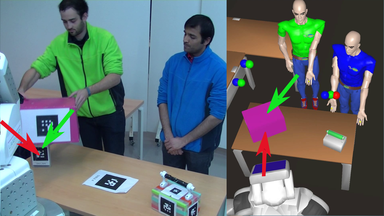
\includegraphics[width=0.99\textwidth]{./SallyAndAnne/2mas.png}\label{startSA}}
  \end{center}
\end{figure*}
    
\clearpage
    \begin{figure*}[ht!]
  \begin{center}
    \subfigure[Greg part et Bob enlève le livre blanc de la boîte rose.]{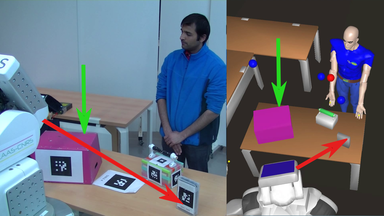
\includegraphics[width=0.99\textwidth]{./SallyAndAnne/3mas.png}\label{middleSA}}
    \subfigure[Bob met le livre blanc sous la petite boîte, puis Greg revient. Le robot est capable de comprendre que Greg croit que le livre est sous la boîte rose.]{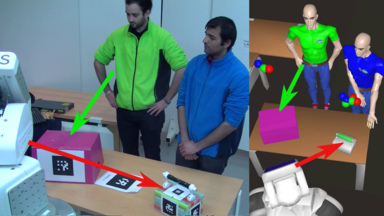
\includegraphics[width=0.99\textwidth]{./SallyAndAnne/4mas.png}\label{endSA}}
 \end{center}
  \caption{Le test de Sally et Anne dans l'environnement réel (partie de gauche) et tel qu'il est perçu par le robot (partie de droite). Pour aider à la compréhension, nous montrons explicitement les croyances concernant la position du livre blanc. Les croyances de Greg sont indiquées avec des flèches vertes et celles du robot avec des flèches rouges.
Les petites sphères de couleur dans l'environnement perçu sont utilisées comme des indications sur l'accessibilité d'un objet pour un agent.}
  \label{SA}
\end{figure*}

Dans le premier scénario, afin de tester notre système et d'illustrer la capacité du robot à détecter les croyances fausses/divergentes sur la position d'un objet nous avons décidé de le soumettre à une adaptation du test de Sally et Anne, déjà présenté par la figure \ref{fig:sallyAndAnne}. Dans notre expérience, deux utilisateurs Greg (en vert) et Bob (en bleu) font face au robot.
La scène est composée d'un livre blanc et de deux boîtes se trouvant sur une table \ref{initSA}).
Greg met le livre blanc sous la boîte rose (\ref{startSA}). Puis Greg quitte la scène. Pendant que Greg est parti, Bob prend le livre blanc et le met sous la petite boîte. (\ref{middleSA} et \ref{endSA}).
Puis, quand Greg revient, nous demandons au robot où Greg pense que le livre se trouve.





Nous allons présenter ci-dessous quelques faits symboliques intéressants pour Greg et le robot correspondants à la situation décrite en \ref{endSA}. Les croyances de Bob restent identiques à celles du robot et ne seront donc pas affichées par simplification.
\begin{scriptsize}
\begin{verbatim}
          ROBOT                         GREG
GREG canSee PINK_BOX  TRUE      GREG canSee PINK_BOX  TRUE
GREG canSee SMALL_BOX TRUE      GREG canSee SMALL_BOX TRUE
GREG canSee BOOK      FALSE     GREG canSee BOOK      FALSE
BOOK isIn   SMALL_BOX TRUE      BOOK isIn   PINK_BOX  TRUE

\end{verbatim}
\end{scriptsize}

Comme le robot sait que le livre n'est pas visible par Greg, il n'a pas mis à jour ses croyances concernant la position de cet objet. Avec l'aide du système d'estimation de la situation maintenant le modèle de croyance des agents, le robot est capable d'observer que, comme Greg ne peut observer ce qui a changé, il a une croyance divergente sur la position de l'objet. Si l'homme et le robot doivent accomplir une tâche impliquant cet objet, le robot sera capable de savoir qu'il doit informer l'homme de la position de l'objet.

\subsubsection{Gestion de croyances divergentes}


Pour aller plus loin et illustrer les trois différentes situations présentées en section \ref{sec:divB}, nous avons tourné un autre scénario illustré par la figure \ref{divB}. Dans cette deuxième expérimentation, deux utilisateurs, Greg et Bob, font face au robot. Ils ont un livre blanc et une boîte blanche qui servira pour faire de l'occlusion visuelle (\ref{initDB}).
Une fois que Bob part (\ref{startDB}), Greg prend le livre blanc et le met derrière la boîte blanche pour qu'il ne soit pas visible du point de vue humain (\ref{startDB}).
Puis Greg part et Bob revient. Le robot est capable d'inférer que, comme le livre blanc est caché, Bob ne sait pas où il se trouve. Toutefois, Bob peut voir que le livre n'est plus là où il pensait être. Cette information manquante est représentée par une sphère transparente à l'emplacement où Bob pensait trouver l'objet (\ref{lackBobDB}).


\begin{figure*}[ht!]
  \begin{center}
    \subfigure[Greg (en vert) et Bob (en bleu) font face au robot. Ils connaissent la position de chaque objet.]{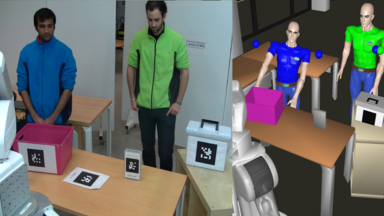
\includegraphics[width=0.79\textwidth]{./DivBFull/1ms.png}\label{initDB}}
    \subfigure[Bob part, Greg met le livre blanc derrière la boîte blanche.]{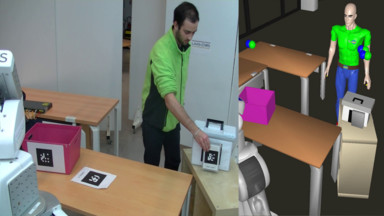
\includegraphics[width=0.79\textwidth]{./DivBFull/2ms.png}\label{startDB}}
    \subfigure[Greg part et Bob revient. Bob ignore la position du livre blanc. Le robot est au courant de ce manque d'information (une sphère bleue transparente représente la dernière croyance de Bob concernant la position du livre blanc).]{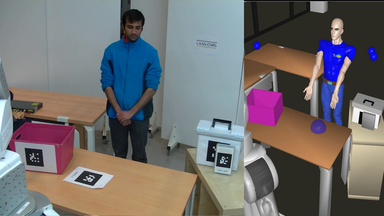
\includegraphics[width=0.79\textwidth]{./DivBFull/3ms.png}\label{lackBobDB}}
    \end{center}
\end{figure*}
    
\clearpage
    \begin{figure*}[ht!]
  \begin{center}
    \subfigure[Bob regarde derrière la boîte blanche (et donc met à jour ses croyances) et prend le livre blanc. ]{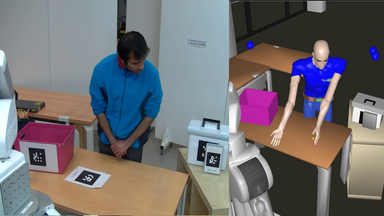
\includegraphics[width=0.61\textwidth]{./DivBFull/4ms.png}\label{updateBobDB}}
   \vspace{-5pt}
    \subfigure[Bob part avec le livre blanc, puis Greg revient. Greg pense toujours que le livre blanc est derrière la boîte blanche. Le robot est au courant de cette croyance divergente (Une sphère opaque verte représente la croyance actuelle de Greg concernant la position du livre blanc).]{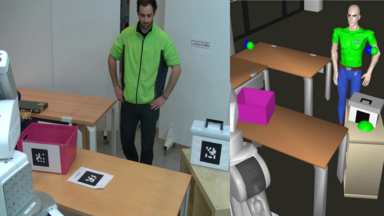
\includegraphics[width=0.61\textwidth]{./DivBFull/6ms.png}\label{GregDB}}
   \vspace{-5pt}
    \subfigure[Greg regarde derrière la boîte blanche et est alors informé que sa croyance est erronée mais ne connaît pas la nouvelle position de l'objet (la sphère devient transparente).]
   {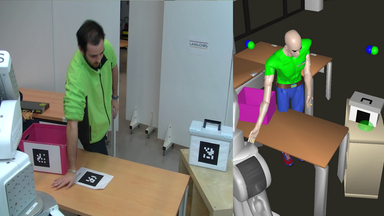
\includegraphics[width=0.61\textwidth]{./DivBFull/7ms.png}\label{lackGregDB}}
 \end{center}
   \vspace{-15pt}
  \caption{Scénario de croyances divergentes impliquant un robot Pr2 et deux humains. Le robot est capable de modéliser les croyances de chacun. Les images présentent les étapes du scénario dans l'environnement réel (partie de gauche) et tel qu'il est perçu par le robot (partie de droite).}
  \label{divB}
\end{figure*}
   \vspace{-14pt}
\clearpage

Ci-dessous sont représentés quelques faits symboliques concernant les croyances de Bob et du robot tel que le robot les modélise.

\begin{scriptsize}
\begin{verbatim}
          ROBOT                                    BOB
ROBOT  canSee   WHITE_BOX TRUE          ROBOT  canSee WHITE_BOX   TRUE    
BOB    canSee   WHITE_BOX TRUE          BOB    canSee   WHITE_BOX TRUE
BOB    canSee   BOOK      FALSE         BOB    canSee   BOOK      FALSE
BOOK   isNextTo WHITE_BOX TRUE          BOOK   location           unknown
\end{verbatim}
\end{scriptsize}

A l'étape suivante, Bob regarde derrière la boîte blanche et met à jour ses croyances (\ref{updateBobDB}). Les croyances de Bob et du robot sont alors identiques.
Puis il prend le livre blanc et s'en va. Lorsque Greg revient, comme l'objet était caché auparavant et n'est toujours pas visible, le robot est capable de comprendre que Greg n'a pas mis à jour ses croyances et a donc une croyance erronée sur la position du livre blanc. Cette croyance erronée est représentée par une sphère opaque à l'emplacement où Greg pense que le livre se trouve (\ref{GregDB}).

Ci-dessous sont représentés quelques faits symboliques concernant les croyances de Greg et du robot tel que le robot les modélise à ce moment là.

\begin{scriptsize}
\begin{verbatim}
          ROBOT                                        GREG
ROBOT  canSee    WHITE_BOX  TRUE          ROBOT  canSee   WHITE_BOX   TRUE    
GREG   canSee    WHITE_BOX  TRUE          GREG   canSee   WHITE_BOX   TRUE
GREG   canSee    BOOK       FALSE         GREG   canSee   BOOK        FALSE
BOB    hasInHand BOOK       TRUE          BOOK   isNextTo WHITE_BOX
\end{verbatim}
\end{scriptsize}

Puis Greg regarde derrière la boîte blanche. Dès qu'il voit que le livre n'y est pas, il n'a plus de croyance divergente mais il ignore toujours où se trouve le livre. Comme le robot a suivi cette action d'observation, il a mis à jour le modèle d'état mental de Greg. La sphère représentant la croyance de Greg sur la position du livre est alors devenue transparente (\ref{lackGregDB}).

Ci-dessous sont représentés quelques faits symboliques concernant les croyances de Greg et du robot tel que le robot les modélise à ce moment là.

\begin{scriptsize}
\begin{verbatim}
          ROBOT                                        GREG
ROBOT  canSee    WHITE_BOX  TRUE          ROBOT  canSee   WHITE_BOX   TRUE    
GREG   canSee    WHITE_BOX  TRUE          GREG   canSee   WHITE_BOX   TRUE
GREG   canSee    BOOK       FALSE         GREG   canSee   BOOK        FALSE
BOB    hasInHand BOOK       TRUE          BOOK   location             unknown
\end{verbatim}
\end{scriptsize}


Sans notre algorithme, à chaque étape le robot penserait que les humains ont la même croyance que lui concernant la position des objets (à savoir que l'humain connaît la nouvelle position de l'objet).


\section{Conclusion}
%TODO
Nous avons montré comment en ajoutant des calculs géométriques à notre système d'évaluation de la situation il nous est possible de mettre en place un suivi de la situation spatiale de l'homme et de ses affordances en terme de visibilité et d'accessibilité des éléments.

Basé sur cette visibilité, nous avons montré comment il est possible de modéliser et de maintenir un état de croyance pour chaque agent. Ceci est réalisé en utilisant des règles fondées sur l'observabilité des propriétés et sur la possibilité pour l'agent concerné de voir l'entité liée à la propriété.
Nous avons également conduit une étude permettant de valider et mettre en pratique la capacité de prise de perspective conceptuelle du robot, notamment en faisant passer une réplique du test de Sally et Anne.

Ces capacités de prise de perspective et de raisonnement sur l'état des agents en terme de situation spatiale, de capacité perceptive et d'état de croyance sont essentielles pour une bonne compréhension de l'homme.
Dans le chapitre suivant, nous montrerons comment la prise de perspective de niveau aide à l'identification de référent pour le dialogue situé homme robot et comment la prise de perspective de niveau deux peut être intégrée à un système de dialogue pour donner un aspect "situé" et ainsi en améliorer l'efficacité et le taux de succès.

Dans le chapitre \ref{chapter4}, la capacité de prise de perspective conceptuelle
est utilisée pour interpréter convenablement les actions d'un homme afin d'en déduire son intention et de donner un comportement proactif au robot.




%REDIT avec chapter3?
% \subsubsection{Dialog disambiguation}


% Now we will show how dialog could benefits from
%   our system. 
% At the end of the scenario of fig  ~\ref{divB}, Bob left with the white book. The robot was able to see this action by using the monitoring spheres. Now, let's assume that in
% addition to this setup, a black book stands on the table but is hidden by the pink box on Bob's side. So the black book is not visible by
% Bob and is visible by the robot.
% Consequently, if Bob asks the robot "where is the book?", as the robot knows Bob took the white one, even if both books are currently not visible by Bob it understands that Bob speaks about the black book. The robot will answer: "It is on the table behind the pink box".
% Such dialog ability is only possible if the robot
% holds correct assumption concerning human's knowledge as done by our
% system. Without the temporal reasonning on human actions, robot would have to ask "which book are you talking about?".

% %comment dans le texte, essaie de bien grouper chacun des
% %  exemples dans un paragraphe, si tu regardes le résultat pour le
% %  moment, c'est pas évident de voir la séparation

% Now, come back to the end of the scenario of fig
%   ~\ref{divB} where Greg has a wrong belief about the white book's
%   position (symbolized by an opaque green sphere). Seeing Greg trying
%   to have a look behind the white box, the robot can infer that he's
%   looking for the white book. Consequently, it can say proactively :
%   "The object you are looking for was taken by Bob''. Such proactive
%   dialog ability is possible with the help of our system because it
%   allows to infer human's intention from human's (wrong or lack of)
%   belief and to talk proactively to the human to correct it.
% % comment fin du second exemple, mettre la phrase de
% %  conclusion à part


% This level of human understanding allows the robot to interact in a more natural way with humans.









% TODO: chapter on intention -> put here?

\ifdefined\included
\else
\bibliographystyle{acm}
\bibliography{These}
\end{document}
\fi

\ifdefined\included
\else
\documentclass[a4paper,11pt,twoside]{StyleThese}
\usepackage{amsmath,amssymb}             % AMS Math
\usepackage[french]{babel}
\usepackage[utf8]{inputenc}
\usepackage[T1]{fontenc}
\usepackage{tabularx}
%\usepackage{tabular}
\usepackage{multirow}


\usepackage[tight,footnotesize]{subfigure}
\usepackage{algorithm} %To allow algorithm environment
\usepackage{algpseudocode} %Provides algorithmic environment

\usepackage{hhline}
\usepackage[left=1.5in,right=1.3in,top=1.1in,bottom=1.1in,includefoot,includehead,headheight=13.6pt]{geometry}
\renewcommand{\baselinestretch}{1.05}

% Table of contents for each chapter

\usepackage[nottoc, notlof, notlot]{tocbibind}
\usepackage[french]{minitoc}
\setcounter{minitocdepth}{2}
\mtcindent=15pt
% Use \minitoc where to put a table of contents

\usepackage{aecompl}

% Glossary / list of abbreviations

\usepackage[intoc]{nomencl}
\renewcommand{\nomname}{Liste des Abréviations}

\makenomenclature

% My pdf code

\usepackage{ifpdf}

\ifpdf
  \usepackage[pdftex]{graphicx}
  \DeclareGraphicsExtensions{.jpg}
  \usepackage[a4paper,pagebackref,hyperindex=true]{hyperref}
  \usepackage{tikz}
  \usetikzlibrary{arrows,shapes,calc}
\else
  \usepackage{graphicx}
  \DeclareGraphicsExtensions{.ps,.eps}
  \usepackage[a4paper,dvipdfm,pagebackref,hyperindex=true]{hyperref}
\fi

\graphicspath{{.}{images/}}

%nicer backref links
\renewcommand*{\backref}[1]{}
\renewcommand*{\backrefalt}[4]{%
\ifcase #1 %
(Non cité.)%
\or
(Cité en page~#2.)%
\else
(Cité en pages~#2.)%
\fi}
\renewcommand*{\backrefsep}{, }
\renewcommand*{\backreftwosep}{ et~}
\renewcommand*{\backreflastsep}{ et~}

% Links in pdf
\usepackage{color}
\definecolor{linkcol}{rgb}{0,0,0.4} 
\definecolor{citecol}{rgb}{0.5,0,0} 
\definecolor{linkcol}{rgb}{0,0,0} 
\definecolor{citecol}{rgb}{0,0,0}
% Change this to change the informations included in the pdf file

\hypersetup
{
bookmarksopen=true,
pdftitle="Évaluation de la sécurité des équipements grand public connectés à Internet",
pdfauthor="Yann BACHY", %auteur du document
pdfsubject="Thèse", %sujet du document
%pdftoolbar=false, %barre d'outils non visible
pdfmenubar=true, %barre de menu visible
pdfhighlight=/O, %effet d'un clic sur un lien hypertexte
colorlinks=true, %couleurs sur les liens hypertextes
pdfpagemode=None, %aucun mode de page
pdfpagelayout=SinglePage, %ouverture en simple page
pdffitwindow=true, %pages ouvertes entierement dans toute la fenetre
linkcolor=linkcol, %couleur des liens hypertextes internes
citecolor=citecol, %couleur des liens pour les citations
urlcolor=linkcol %couleur des liens pour les url
}

% definitions.
% -------------------

\setcounter{secnumdepth}{3}
\setcounter{tocdepth}{2}

% Some useful commands and shortcut for maths:  partial derivative and stuff

\newcommand{\pd}[2]{\frac{\partial #1}{\partial #2}}
\def\abs{\operatorname{abs}}
\def\argmax{\operatornamewithlimits{arg\,max}}
\def\argmin{\operatornamewithlimits{arg\,min}}
\def\diag{\operatorname{Diag}}
\newcommand{\eqRef}[1]{(\ref{#1})}

\usepackage{rotating}                    % Sideways of figures & tables
%\usepackage{bibunits}
%\usepackage[sectionbib]{chapterbib}          % Cross-reference package (Natural BiB)
%\usepackage{natbib}                  % Put References at the end of each chapter
                                         % Do not put 'sectionbib' option here.
                                         % Sectionbib option in 'natbib' will do.
\usepackage{fancyhdr}                    % Fancy Header and Footer

% \usepackage{txfonts}                     % Public Times New Roman text & math font
  
%%% Fancy Header %%%%%%%%%%%%%%%%%%%%%%%%%%%%%%%%%%%%%%%%%%%%%%%%%%%%%%%%%%%%%%%%%%
% Fancy Header Style Options

\pagestyle{fancy}                       % Sets fancy header and footer
\fancyfoot{}                            % Delete current footer settings

%\renewcommand{\chaptermark}[1]{         % Lower Case Chapter marker style
%  \markboth{\chaptername\ \thechapter.\ #1}}{}} %

%\renewcommand{\sectionmark}[1]{         % Lower case Section marker style
%  \markright{\thesection.\ #1}}         %

\fancyhead[LE,RO]{\bfseries\thepage}    % Page number (boldface) in left on even
% pages and right on odd pages
\fancyhead[RE]{\bfseries\nouppercase{\leftmark}}      % Chapter in the right on even pages
\fancyhead[LO]{\bfseries\nouppercase{\rightmark}}     % Section in the left on odd pages

\let\headruleORIG\headrule
\renewcommand{\headrule}{\color{black} \headruleORIG}
\renewcommand{\headrulewidth}{1.0pt}
\usepackage{colortbl}
\arrayrulecolor{black}

\fancypagestyle{plain}{
  \fancyhead{}
  \fancyfoot{}
  \renewcommand{\headrulewidth}{0pt}
}

%\usepackage{MyAlgorithm}
%\usepackage[noend]{MyAlgorithmic}
\usepackage[ED=MITT - STICIA, Ets=INP]{tlsflyleaf}
%%% Clear Header %%%%%%%%%%%%%%%%%%%%%%%%%%%%%%%%%%%%%%%%%%%%%%%%%%%%%%%%%%%%%%%%%%
% Clear Header Style on the Last Empty Odd pages
\makeatletter

\def\cleardoublepage{\clearpage\if@twoside \ifodd\c@page\else%
  \hbox{}%
  \thispagestyle{empty}%              % Empty header styles
  \newpage%
  \if@twocolumn\hbox{}\newpage\fi\fi\fi}

\makeatother
 
%%%%%%%%%%%%%%%%%%%%%%%%%%%%%%%%%%%%%%%%%%%%%%%%%%%%%%%%%%%%%%%%%%%%%%%%%%%%%%% 
% Prints your review date and 'Draft Version' (From Josullvn, CS, CMU)
\newcommand{\reviewtimetoday}[2]{\special{!userdict begin
    /bop-hook{gsave 20 710 translate 45 rotate 0.8 setgray
      /Times-Roman findfont 12 scalefont setfont 0 0   moveto (#1) show
      0 -12 moveto (#2) show grestore}def end}}
% You can turn on or off this option.
% \reviewtimetoday{\today}{Draft Version}
%%%%%%%%%%%%%%%%%%%%%%%%%%%%%%%%%%%%%%%%%%%%%%%%%%%%%%%%%%%%%%%%%%%%%%%%%%%%%%% 

\newenvironment{maxime}[1]
{
\vspace*{0cm}
\hfill
\begin{minipage}{0.5\textwidth}%
%\rule[0.5ex]{\textwidth}{0.1mm}\\%
\hrulefill $\:$ {\bf #1}\\
%\vspace*{-0.25cm}
\it 
}%
{%

\hrulefill
\vspace*{0.5cm}%
\end{minipage}
}

\let\minitocORIG\minitoc
\renewcommand{\minitoc}{\minitocORIG \vspace{1.5em}}

\usepackage{multirow}
%\usepackage{slashbox}

\newenvironment{bulletList}%
{ \begin{list}%
	{$\bullet$}%
	{\setlength{\labelwidth}{25pt}%
	 \setlength{\leftmargin}{30pt}%
	 \setlength{\itemsep}{\parsep}}}%
{ \end{list} }

\newtheorem{definition}{Définition}
\renewcommand{\epsilon}{\varepsilon}

% centered page environment

\newenvironment{vcenterpage}
{\newpage\vspace*{\fill}\thispagestyle{empty}\renewcommand{\headrulewidth}{0pt}}
{\vspace*{\fill}}

\usepackage{tablefootnote}
\sloppy
\begin{document}
\setcounter{chapter}{2} %% Numéro du chapitre précédent ;)
\dominitoc
\faketableofcontents
\fi

\chapter{Vers un Dialogue Situé Homme-Robot}
\label{chapter3}
\minitoc

\section{Contexte}

\subsection{Introduction}
%intro + related work
L'une des compétences essentielles pour interagir convenablement avec l'homme est de fournir des moyens d'assurer la compréhension mutuelle dans le contexte situé de l'activité jointe. Le robot et l'humain doivent avoir des références aux éléments de l'environnements qui soient communes (common ground), ce qui signifi qu'ils doivent pouvoir identifier, dans leur propre représentation du monde, les actions, les entités (humains, robots ou objets) et les propriétés énnoncées par leur interlocuteur.
%TODO biblio on grounding / situated dialogue / reference generation

Les systèmes robotiques reposent sur les capteurs pour reconnaître et localiser les entités afin de construire l'état du monde. Ces capteurs produisent des coordonnées pour positionner les entités par rapport à un repère donné. Par exemple, une caméra stéréo avec un logiciel de reconnaissance peut permettre de savoir qu'une tasse est à une position donnée  $x$, $y$, $z$ avec une orientation $\theta$, $\phi$, $\psi$.
Les humains quand à eux, utilisent les relations spatiales entre les éléments pour décrire leur position. Pour indiquer la position de la tasse, l'humain dirait par exemple qu'il se trouve sur la table de la cuisine, sans donner les coordonnées précises.
Pour comprendre les références de l'homme et générer des déclarations compréhensibles, le robot se doit donc de construire une représentation symbolique du monde, basée sur les données géométriques qu'il a collecté par ses capteurs, comme cela a été fait dans \cite{lemaignan2012grounding}.

%We have developed a module based on spatial and temporal reasoning to generate "facts" about the current state of the world \cite{milliez2014framework}. A fact is a property which describes the current state of an entity (e.g. $MUG$ $isNextTo$ $BOTTLE$, $MUG$ $isFull$ $TRUE$). This framework generates facts related to the entities' position and facts about affordances to know, for instance, what is visible or reachable to each agent (human and robot). 
%It also generates facts about agent postures to know if an agent is pointing toward an object or where an agent is looking. When the robot tries to understand the human, it should also use these data to improve the information grounding process.

En plus de l'état du monde (qui peut être considéré comme l'état de croyance du robot), pour vraiment comprendre les actes dialoguiques de l'humain dans un contexte situé, il est nécéssaire au robot de comprendre la situation spatiale et mentale de l'homme. En effet, les références qu'il génère dans ses actes communicatifs avec le robot sont suceptible de grandement dépendre de cette situation spatiale ou mentale.

Pour établir ces références communes et comprendre les actes communicatifs humains à la lumières de sa situations, nous avons utilisé notre infrastructure logicielle d'évaluation de la situation, présentée dans les chapitres précédents, dans le cadre d'un projet visant à mettre en place un dialogue situé homme-robot


\subsection{Le projet maRDi}
%Projet MaRDi (thèse Manu)
Ces travaux ont été réalisés dans le cadre du projet MaRDi\footnote{Man-Robot Dialogue - http ://mardi.metz.supelec.fr
} de l’Agence Nationale pour la Recherche (ANR). Il a été financé par l’appel à projet Contenu et Interactions. Les
travaux réalisés ont été faits en collaboration avec le Laboratoire d’Informatique Fondamentale de Lille (LIFL), l’École supérieure d’électricité (Supélec), le groupe Acapela, le Laboratoire Informatique d’Avigon (LIA) et le Laboratoire d’Analyse et d’Architecture des Systèmes (LAAS).
Ce projet a pour axe d’étude l’apport d’une approche "située" du dialogue Homme-
Machine. Le terme "situé" est ici relatif à l’incarnation physique d’un système de dialogue dans une plateforme robotique qui va permettre d’envisager l’intégration d’informations issues des perceptions physiques du robot dans le contexte de l’interaction pour espérer compléter ou lever des ambiguïtés introduites par le medium vocal. Ce projet s’inscrit également dans l’utilisation de méthodes d’apprentissage numérique, exploitant les données collectées au travers de la conduite de véritables interactions afin d’améliorer l’efficacité et le naturel du système dans le temps. L’originalité de l’approche est de ne pas considérer les technologies vocales comme disponibles et dissociées de la tâche d’interaction Homme-Robot, mais bel et bien comme moyen d’en améliorer l’expérience et les performances.
Pour atteindre ce but, la Machine doit être capable de maintenir un contexte d’interaction suffisamment riche pour pouvoir être à même de prendre des décisions sur la
suite à donner à celle-ci. Ce contexte intègrera les entrées fournies par l’humain mais
aussi les informations issues des calculs géométriques et des raisonnements effectués à partir de la perception de l’environnement. Sur ces aspects en particulier,
le projet s'appuye sur les recherches menées par le LAAS dans le domaine du raisonnement
spatial et surtout de la prise de perspective, exposés aux chapitres précédents, pour tenter de résoudre des ambiguïtés.
Pour prendre des décisions afin de poursuivre l’interaction, la machine devra s’appuyer sur un contexte de l’interaction (historique, état de l’environnement, etc.) et tenir
compte de son aspect incertain. En effet, dans le cadre situé, le contexte de l’interaction ne peut être considéré comme une donnée sûre car de possibles erreurs ont pu être
introduites par la chaîne de traitement automatique des entrées vocales et visuelles.
%C’est pourquoi les approches stochastiques que nous employons nous permettent de
%modéliser les différentes hypothèses avec leur score de confiance respectif. Ainsi, la
%stratégie d’interaction employée par la machine devra tenir compte des ambiguïtés potentiellement générées et en garder trace tout au long du dialogue. Nous traiterons
%cette problématique par l’utilisation de modèles permettant l’optimisation statistique
%du mécanisme de prise de décision. La faculté d’adaptation à un nouveau profil utilisateur ou plus généralement à des situations contextuelles et dialogiques différentes
%lors de l’apprentissage est une caractéristique désirée qui fera également l’objet de nos
%travaux.
Une fois sa décision prise, le système devra également pouvoir la restituer voca-
lement et physiquement à l’humain. Ainsi il faudra qu’il soit capable de planifier ses
mouvements et ses actions physiques de façon précise pour répondre aux besoins de
l’utilisateur (déplacer un objet, se rendre dans une pièce, etc.), mais également capable
de s’exprimer de façon adéquate pour se faire comprendre par l’utilisateur et lui témoigner de sa compréhension du contexte interactif courant. Pour cela, le robot devra par
exemple adopter des attitudes physiques particulières, ou encore utiliser un timbre de
voix particulier.


\subsection{Scénario associé}

Afin de positionner le scénario dans un cadre naturel et fonctionnel, le choix a été
fait de faire interagir un robot assistant avec un handicapé dans son appartement (aide
à la personne). La personne pourra ainsi, en interagissant avec le robot, lui faire manipuler divers objets. Les objets en quéstion auront des propriétés associées en terme de couleur, de type d'objet (par exemple un DVD), de type de contenu (par exemple science-fiction) et de position et auront un identifiant unique. Pour se faire comprendre
par le robot, l’utilisateur usera principalement de la parole, mais pourra également employer des gestes déictiques (comme le fait de pointer un objet particulier).
Un dialogue multimodal sera ici employé pour pouvoir résoudre les possibles ambiguïtés liées à une précision insuffisante de la requête utilisateur.
Ce dialogue se poursuivra jusqu’à la fin de l’exécution effective de la tâche ou
l’échec de l’interaction. Cette dernière situation peut par exemple être due à un désengagement explicite de l’utilisateur, ou encore à l’exécution d’une commande erronée
de la part du robot. Un exemple d’un tel dialogue multimodal est donné dans le tableau \ref{table:dial}.
Dans ce contexte d’étude nous pourrons également jouer sur la définition de divers
scénarios (configuration de l’environnement, connaissances initiales du robot, position
des agents, etc.) pour rendre l’interaction plus ou moins complexe. Ceci nous permet de
pouvoir tester divers cas d’interactions, notamment dans des configurations "limites" comme celles employées lorsque nous étudierons les tâches de fausses croyances (voir \ref{}).



\begin{table}
\centering
\small
\begin{tabular}{|c|l|}
  \hline
  \multirow{2}{*}{Robot1} & Comment Puis-je vous aider? \\
    & hello() [Greet] \\
    \hline
  \multirow{2}{*}{User1}  & Peux-tu mettre le livre sur ma table de chevet? \\
  	& inform(cmd.action=move, cmd.location=bedroom\_bedsidetable) \\
    \hline
  \multirow{2}{*}{Robot2} & Désolé, mais savez vous où se trouve le livre dont vous me parlez? \\
    & confreq(object.type=book,object.location) [TentRQ] \\
    \hline
  \multirow{2}{*}{User2} & C’est celui là. \\
  	& inform(idobj= ?) + pointsAt BLUE\_BOOK = inform(idobj=BLUE\_BOOK) \\
   \hline
    \multirow{5}{*}{Robot3} & Ok, je vais mettre le livre bleu sur votre table de chevet. \\
     & execute(cmd.action=move,cmd.location=bedroom\_bedsidetable, \\
     & idobj=BLUE\_BOOK,object.location=livingroom\_table,object.type=book, \\
     & object.color=blue) [Execute] \\
     & move(BLUE\_BOOK,livingroom\_table,bedroom\_bedsidetable) \\
    \hline
\end{tabular}
 \caption{Exemple de dialogue multimodal.}
 \label{table:dial}
% \vspace{-20pt}
 \end{table}


% Robot1 >
% Usr1 >
% Robot2 >
% Usr2 >
% Robot3 >
% Comment puis-je vous aider ?
% hello() [Greet]
% Peux-tu mettre le livre sur ma table de chevet ?
% inform(cmd.action=move, cmd.location=bedroom_bedsidetable)
% Désolé, mais où se trouve le livre dont vous me parlez ?
% confreq(object.type=book,object.location) [TentRQ]
% C’est celui là
% inform(idobj= ?) + pointsAt BLUE_BOOK = inform(idobj=BLUE_BOOK)
% Ok, je vais mettre le livre bleu sur votre table de chevet
% execute(cmd.action=move,cmd.location=bedroom_bedsidetable,
% idobj=BLUE_BOOK,object.location=livingroom_table,object.type=book,
% object.color=blue) [Execute]
% move(BLUE_BOOK,livingroom_table,bedroom_bedsidetable)



% \begin{table}
% \centering
% \small
% \begin{tabular}{|c|c|l|}
%   \hline
%   \multirow{3}{*}{R1} & DA & hello() \\
%     & NLG/TTS & Can I help you ?\\
%     \hline
%   \multirow{3}{*}{U1} & ASR & Can you put the book in my bedroom? \\
%   	& SLU & inform(action=move,desc=in,room=bedroom)\\
%     \hline
%   \multirow{3}{*}{R2} & DA & confreq(type=book,position) \\
%     & NLG/TTS & Sorry but where is the book you are talking about?\\
%     \hline
%   \multirow{3}{*}{U3} & ASR & I am talking about this one \\
%   	& SLU & inform(idobj=?)\\
%     & GRU & pointsAt BLUE\_BOOK 1395848705.31\\
%    \hline
%     \multirow{4}{*}{R3} & & execute(action=move,destination=bedroom\_bedsidetable,\\
%      & DA & idobj=BLUE\_BOOK,position=livingroom\_table,type=book,\\
%     & &color=blue) \\
%     & NVBP/MC & move(BLUE\_BOOK,livingroom\_table,bedroom\_bedsidetable)\\
%     & NLG/TTS & Ok, I will put the blue book on your bedside table\\
%     \hline
% \end{tabular}
%  \caption{Example of a multimodal dialogue.}
%  \label{table:hri-example}
%  \vspace{-20pt}
%  \end{table}


Le robot utilisé est le PR2. L'appartement choisi pour conduire nos expériences est la réplique taille réelle
d’un 3 pièces (salon, cuisine, chambre) présent dans les locaux du LAAS-CNRS et dont une modélisation fidèle a été faite sur simulateur 3D.
Dans chaque pièce se trouvent des meubles, sur lesquels des objets peuvent être posés. Cet environnement est représenté à la figure \ref{fig:env}







\begin{figure}[ht!]
 \centering
  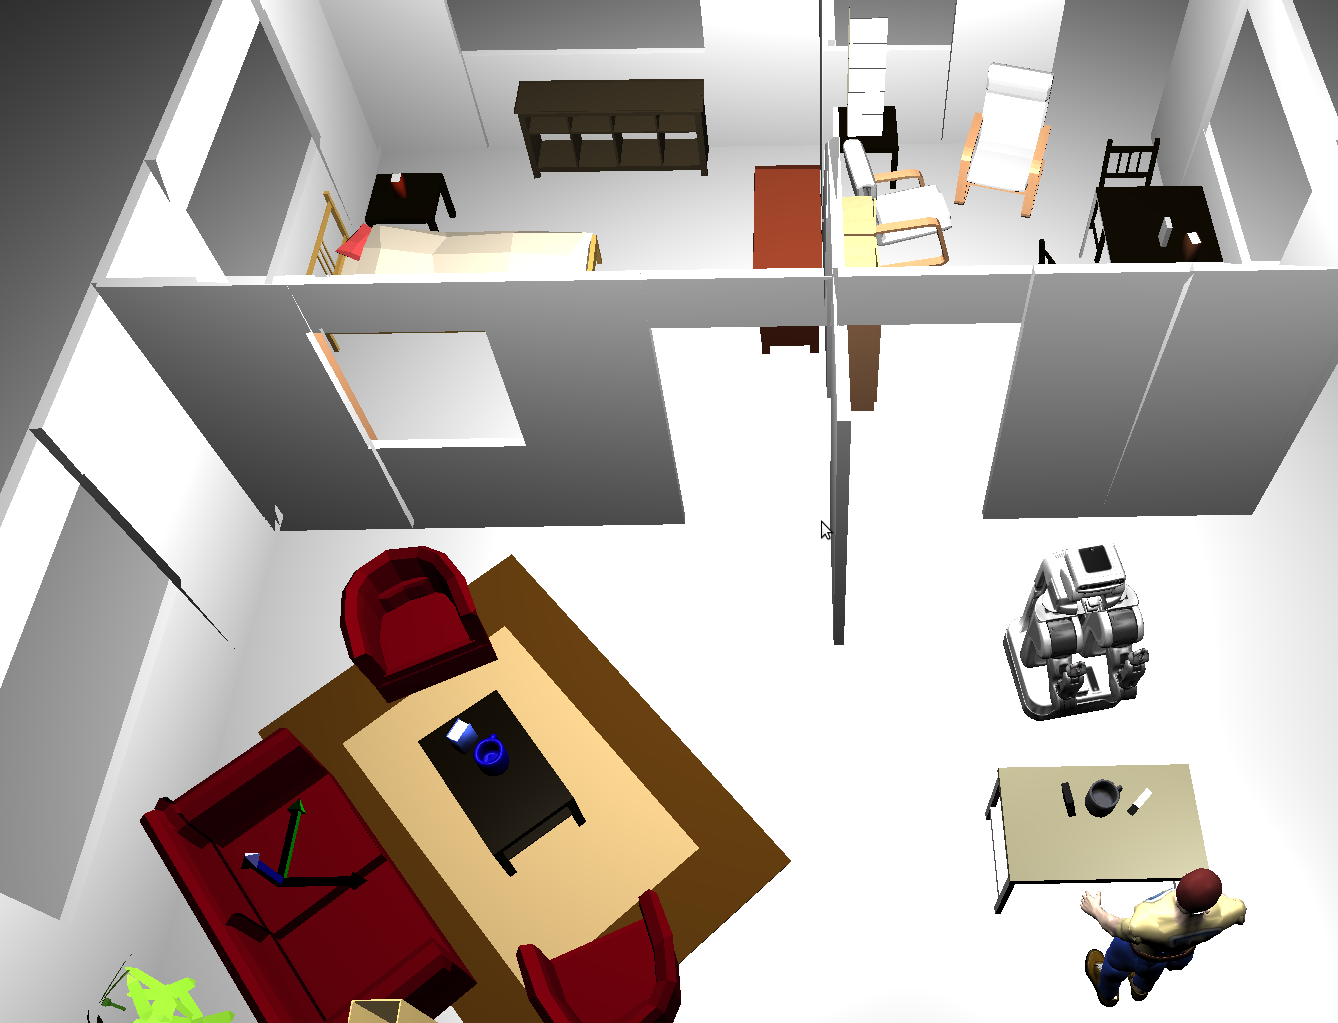
\includegraphics[width=0.89\linewidth]{./img/LAASMORSE.png} 
  \caption {Représentation tridimensionnelle de l'environnement utilisé.}
  \label{fig:env}
\end{figure}


\section{Les trois phases de l'intéraction}



L'architecture mise en place pour la réalisation de l'interaction contient divers modules qui interviennent à différentes étapes.
Il est possible ici de distinguer 3 phases. 

\begin{itemize}
\item La première phase fait intervenir les éléments permettant le bon fonctionnement du dialogue situé afin de définir le but de l'utilisateur.
\item La deuxième phase consiste à transmettre le but au planificateur afin que celui-ci puisse, en utilisant les informations sur la configuration actuelle de l'environnement, trouver un plan qui permette d'atteindre le but. 
\item La dernière fait intervenir la supervision qui pilote la planification de trajéctoire et de mouvement et contrôle le bon déroulement de l'execution de la tâche à accomplir.
\end{itemize}

Ces différentes phases font intervenir divers éléments du système.
Nous allons détailler les procésus impliqués dans chaque phase et les échanges de données.

\subsection{Détermination du but utilisateur}
Durant cette phase, l'humain et le robot dialoguent afin de déterminer le but de l'utilisateur. Pour expliquer les différents flux, nous nous appuyerons sur la figure \ref{fig:phase1}.


\begin{figure}[ht!]
 \centering
  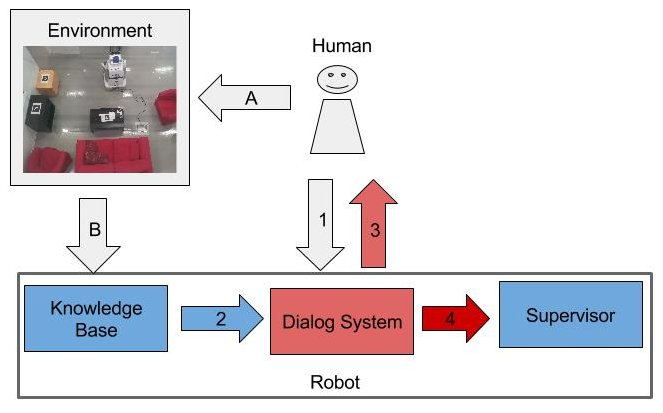
\includegraphics[width=0.99\linewidth]{./img/phase1color.jpg} 
  \caption {Schéma des différents composants et flux intervenant dans la phase de détermination du but utilisateur.}
  \label{fig:phase1}
\end{figure}

Dans cette première phase, l'homme peut en permanance agir sur l'environnement (flux A). L'environnement étant en permanance mis à jour par notre système d'évaluation de la situation (flux B), la base de connaissance sera mise à jour en conséquence.
Lors de cette phase d'estimation du but utilisateur, l'homme parle au robot (flux 1) en utilisant potentiellement des signes pour accompagner sa parole. Le système de dialogue du robot interprète les dires de l'homme en utilisant sa base de connaissance (flux 2) et génère une réponse appropriée à l'homme, par exemple en lui demandant une précision sur la tâche à accomplir (flux 3). L'opération est répétée (flux 1, 2, 3) juqu'à ce que le système de dialogue ait une représentation du fait avec tous les champs nécéssaires. Dans ce cas, à la place de répondre à l'homme (flux 3) le système de dialogue envoit le but de l'utilisateur au superviseur (flux 4). La phase de détermination de but est alors finie et l'interaction entre dans la phase d'élaboration de plan permettant de résoudre le but utilisateur. 

\subsection{Élaboration de plan}
Durant cette phase, le robot cherche un plan permettant de résoudre le but de l'utilisateur. Pour expliquer les différents flux, nous nous appuyerons sur la figure \ref{fig:phase2}.




\begin{figure}[ht!]
 \centering
  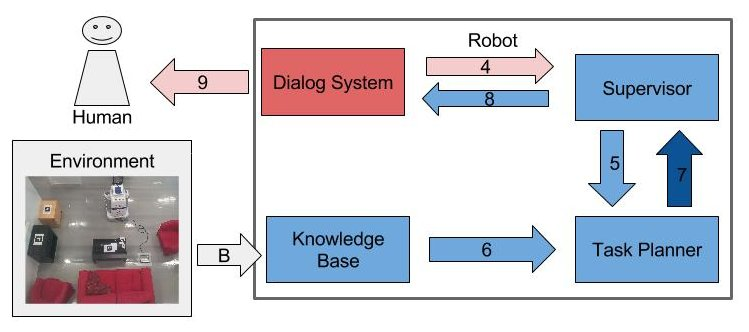
\includegraphics[width=0.99\linewidth]{./img/phase2color.jpg} 
  \caption {Schéma des différents composants et flux intervenant dans la phase d'élaboration de plan pour résoudre le but utilisateur.}
  \label{fig:phase2}
\end{figure}

À la fin de la phase de détermination du but utilistateur, le système de dialogue transmets ce but au superviseur (flux 4). Le superviseur par la suite transmets ce but au planificateur de tâche (flux 5). Le planificateur de tâche utilise la représentation symbolique de l'environnement, contenu dans la base de connaissance et provenant des calculs et raisonnements fait par le système d'évaluation de la situation, pour avoir connaissance de l'état du monde actuel et générer un plan permettant d'atteindre le but souhaité par l'utilisateur. Le planificateur de tâche renvoit un message au superviseur lui informant du succès ou de l'échec de la planification (flux 7). En cas d'échec, le superviseur informe le système de dialogue (flux 8) qui à son tour informe l'humain de l'impossibilité d'execution du plan (flux 9).
L'interaction retourne alors à la phase précédente afin de tenter d'établir un but utilisateur qui soit réalisable. 
Dans le cas où la planification est un succès (un plan a été trouvé), le plan est envoyé au superviseur (flux 7) et l'interaction peu passer à la phase d'execution du plan.


\subsection{Exécution du plan}
Durant cette phase, le robot cherche à exécuter les tâches du plan permettant d'accomplir le but de l'utilisateur. Pour expliquer les différents flux, nous nous appuyerons sur la figure \ref{fig:phase3}.




\begin{figure}[ht!]
 \centering
  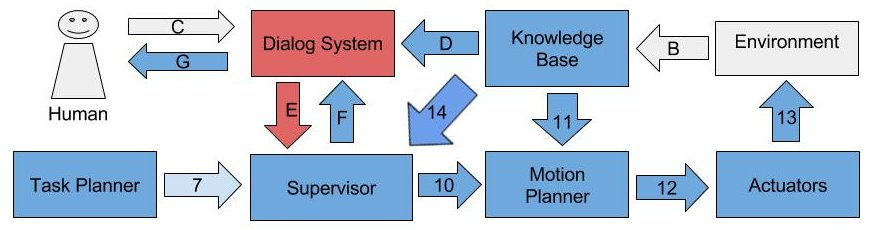
\includegraphics[width=0.99\linewidth]{./img/phase3color.jpg} 
  \caption {Schéma des différents composants et flux intervenant dans la phase d'exécution de plan pour accomplir le but utilisateur.}
  \label{fig:phase3}
\end{figure}

À la fin de la phase précédente, le planificateur de tâche transmets le plan à la supervision (flux 7). Le composant de supervision gère l'execution de la tâche grâce à la planification de mouvements (flux 10) qui envoye des commandes aux actuateurs du robot (flux 12). Le superviseur contrôle la bonne execution du plan à l'aide des éventuels retour d'erreur des différents composants et en surveillant l'évolution de l'état du monde (flux 14). Durant cette execution, l'homme peut à tout moment dialogué avec le système (flux C) afin de:
\begin{itemize}
\item Demander une information sur l'environnement. Au quel cas le système de dialogue utilise la base de connaissance (flux D) pour répondre au mieux à l'humain (flux G).
\item S'enquérir de l'état d'avancement de la tâche ou de l'action courante du robot. Au quel cas le système de dialogue envoye une requète correspondante au superviseur (flux E) qui transmets cette information (flux F) et qui est transmise à l'homme par le système de dialogue (flux G).
\item Demander un abandon de la tâche ou un changement de plan. Le système de dialogue transmets alors cette requète au superviseur (flux E). Puis en cas d'abandon, l'interaction retourne en phase de détermination de but utilisateur ou en cas de changement de plan, en phase d'élaboration d'un nouveau plan prenant en compte les demandes de l'utilisateur. Cette dernière fonctionnalité est présentée plus en détail en section \ref{sec:planning}.
\end{itemize}

%mais ne sont pas nécéssairement séquencées de façon ordonée. En effet, durant la phase d'identification du but utilisateur, il est possible qu'un but "intermédiaire" soit généré par le robot afin de faire avancer le dialogue et l'identification du but final de l'utilisateur. Par exemple, le robot peux décider d'aller verifier un fait en se déplaçant dans l'appartement, soulevé une boîte pour montrer à l'homme ce qu'il s'y trouve... Il est donc possible que le robot ait à planifier ou à agir pour mettre à jour son état de connaissance de l'environnement ou celui de l'homme.
%De même, durant la phase de planification, il est possible de faire intervenir le dialogue pour négocier le plan, demander des conseils à l'homme ou l'informer de l'échec de la planification.
%Enfin, durant l'execution, il est nécéssaire que le robot informe l'homme de l'évolution de la tâche. Le robot doit également pouvoir proposer une alternative au but de l'homme si le but donné par l'homme n'est pas atteignable.
%Pour améliorer l'intéraction, l'homme devrait également pouvoir demander des informations au robot ou lui demander d'abandonner la tâche pendant l'execution.




\section{Architecture du système de dialogue situé}

Dans cette partie, nous allons aller plus loin dans l'explication du système de dialogue situé, intervenant principalement dans la première phase, en détaillant les différents modules qui entrent en jeu lors de la détermination du but utilisateur. Nous allons notamment détailler comment le système de dialogue est enrichit en utilisant le contexte de l'intéraction et la base de fait maintenue par le système d'évaluation de la situation.

Nous présentons à la figure \ref{fig:archiphase1}, l'architecture détaillée mise en place pour la première phase d'intéraction. Nous nous baserons sur cette figure pour expliquer les différents flux, ainsi que les différents modules qui permettent le bon fonctionnement du dialogue situé.


\begin{figure}[ht!]
 \centering
  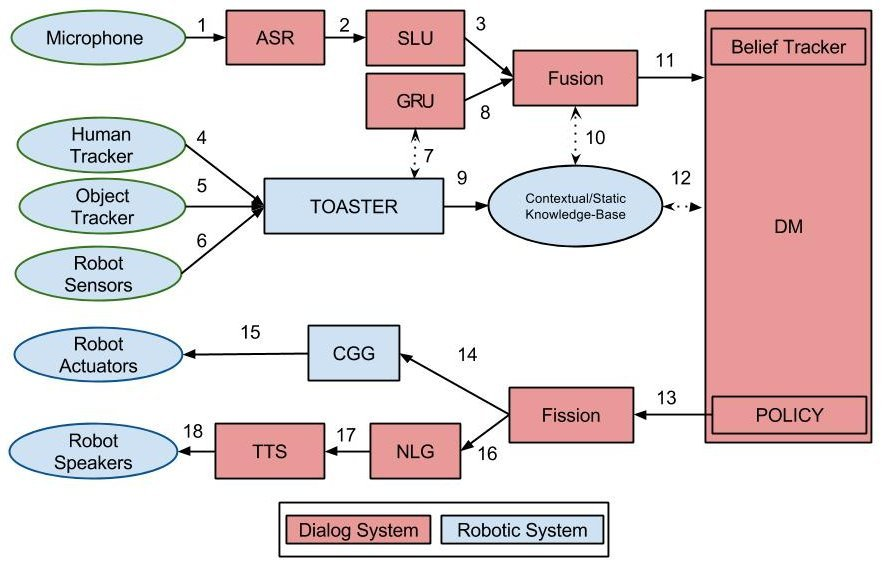
\includegraphics[width=0.89\linewidth]{./img/archiphase1.jpg} 
  \caption {Architecture détaillant les différents composant du système de dialogue situé.}
  \label{fig:archiphase1}
\end{figure}

Il est possible d'identifier plusieurs sous parties dans cette architecture.
La première est en charge des entrées multimodales de l'utilisateur. Une deuxième partie est responsable de l'aquisition et du maintient de l'état du monde ainsi que de la génération de données symboliques. Le gestionnaire de dialogue, ou DM (Dialogue Manager) permets de décider, en fonction des entrées interprétées de l'utilisateur et du contexte de l'intéraction de la réponse donnée par le robot afin de parvenir à déterminer le but.
La dernière partie s'attache à restituer sous forme multimodale la sortie du système de dialogue décidée par le gestionnaire de dialogue.
Certains modules relevant d'avantage du dialogue proprement parlé que de l'usage du système d'évaluation de la situation, une description brève en sera donnée. Pour plus de renseignements sur ces modules et une déscription plus exhaustive de la partie dialogue, nous invitons le lécteur à consulter les articles \cite{} ainsi que la thèse 


%TODO ref au travail de Manu

\subsection{Entrées multimodales utilisateur}
\label{sec:entréesDial}
Cette première partie permets d'aquérir et d'interpréter les entrées multimodales de l'homme en fonction du contexte de l'intéraction. En effet, l’utilisateur peut faire l’usage de la parole et/ou de
gestes déictiques de façon non contrainte tout au long de l’interaction pour s’adresser
au robot. Une fois la commande de l'utilisateur interprétée, elle est transmise au module de géstion de dialogue. 

Pour aquérir et interpréter les commandes de l'utilisateur, quatre modules sont impliqués.

\begin{itemize}
\item Le module ASR: la reconnaissance de la parole est effectuée grâce au module ASR (Automatic Speech Recognition). Il utilise le flux audio (numéro 1 sur le schéma) provenant du microphone pour traduire ce flux en mots. Ce module est basé sur la Google Web Speech API 3.
\item Le module SLU: l'ASR fournit les mots possiblement prononcés par l'homme au SLU (2). Ces mots sont interprétés par le SLU (Spoken Language Understanding) pour permettre de relier les mots aux concepts mis en jeux.
\item Le module GRU: ce module est chargé de la reconnaissance et la compréhension des gestes déictiques émis par l’utilisateur lors de son tour d’interaction (Gesture Recognition and Understanding). Les gestes de pointage sont détectés et interprétés dynamiquement par notre raisonneur spatial (TOASTER) décrit au premier chapitre de cette thèse. Ce dernier exploite à la fois les coordonnées spatiales des objets (5) et les jointures de l’utilisateur (4) telles que déterminées grâce aux informations issues des capteurs visuels du robot pour savoir si oui ou non un objet est désigné du
doigt par l’utilisateur. Lorsque c’est le cas, un \textit{fait} de la forme \textit{AGENT\_ID pointsAt
OBJECT\_ID} est alors généré et transmis au GRU (7). De plus, ce \textit{fait}, comme tous les faits générés par notre infrastructure de raisonnement géométrique, contient un indicateur temporel. Cela permet de simplifier le mécanisme de
fusion avec les entrées vocales.
%Dans la version actuelle de la plateforme des heuristiques expertes sont employées pour la capture de ces gestes dans SPARK. Cependant, une fois que plus de données auront été collectées, des techniques plus élaborées pourront être envisagées pour les remplacer, comme par exemple celle proposée dans (Rossi et al., 2013) qui fait intervenir un classifieur HMM avec en entrée des données issues d’une caméra RGB-D (coordonnées 3D et angles des jointures du corps de l’utilisateur, état ouvert/fermé de chacune de ses mains, etc.).
\item Le module de fusion: l’objectif du mécanisme de fusion est de combiner les actes de dialogue extraits du
signal de parole utilisateur (3) aux évènements déictiques capturés grâce au module GRU (8).
Pour ce faire, il faut tenir compte à la fois du contexte de l’interaction (positions des
objets dans l’environnement physique, etc.), du niveau de confiance que l’on porte aux
différentes hypothèses unimodales (étant donné qu’elles peuvent être erronées) mais
également à leur marqueur temporel.
La première étape de ce processus consiste donc à déterminer si les hypothèses en
provenance des différentes modalités sont synchrones entre elles et peuvent être fusionnées
ou doivent être considérées séparément. Du fait que la parole est considérée
dans notre étude comme modalité principale de l’utilisateur, les tours d’interaction seront calés sur celui des entrées vocales. Ainsi, comme dans \cite{Holzapfel2004}, seuls les gestes déictiques détectés dans un segment temporel de 20ms avant et après celui du tour de parole courant seront exploités par le mécanisme de fusion. De ce fait, si des hypothèses SLU apparaissent seules ou que les gestes détectés ne leur sont pas synchrones, elles seront directement considérées comme résultat de la fusion. La méthode de fusion retenue ici repose sur la définition d’un ensemble
de règles.
Par exemple si l’utilisateur prononce la
phrase « prends ça » tout en désignant un objet du doigt la fusion a pour rôle principal
d’identifier un candidat valable. Pour ce faire le mécanisme de fusion s’appuie notamment
sur la détection de concepts bas niveau qui témoignent d’un besoin de résolution
de référents dans l’énoncé utilisateur (le mot « ça » dans l’exemple précédent).

La dernière étape du processus consiste à convertir les hypothèses ainsi produites
dans leur représentation sémantique haut niveau pour pouvoir les transmettre au gestionnaire de dialogue (11).
Des heuristiques définies manuellement sont employées pour déterminer les valeurs
des concepts de haut niveau identifiés à partir des hypothèses bas niveau.
\end{itemize}


% \subsection{Entrées Multimodales de l'Utilisateur}

% Dans notre contexte applicatif, l’utilisateur peut faire l’usage de la parole et/ou de
% gestes déictiques de façon non contrainte tout au long de l’interaction pour s’adresser
% au robot. Les quatre modules représentés en orange sur la figure  ont la charge
% d’extraire l’information sémantique résultant de l’analyse des différentes modalités à
% chaque tour de dialogue sous la forme d’une liste unifiée de N-meilleures hypothèses
% d’actes de dialogue utilisateur.

% Nous décrivons ci-dessous les modules mis en jeu pour réaliser la compréhension
% de la parole et des gestes utilisateur avant de décrire la solution retenue pour la fusion
% dans notre étude.

% \subsubsection{Compréhension de la Parole}
% %TODO: rewrite to simplify
% Lorsque l'humain parle, le son de la parole est capturé dans un micro, puis envoyé au module de reconnaissance vocale. La reconnaissance automatique de la parole est effectuée grâce au module ASR (pour Automatic Speech Recognition). Ce module est basé sur la Google Web Speech API 3. Cette dernière
% nous donne l’accès à un ASR grand vocabulaire état de l’art en langue française. Ainsi, à chaque tour de parole utilisateur, une liste des N
% meilleures hypothèses scorées (confiances) de transcription est mise à disposition du
% système (N = 5 dans nos travaux).

% L'ASR fournit donc les mots possiblement prononcés par l'homme. Cependant, ces mots doivent être interprétés pour permettre de relier les mots aux concepts mis en jeux. Cette compréhension est faite par le SLU.
% L'implémentation du module SLU est réalisé par le LIA. 
% Plus de détails sont disponibles dans %TODO donner une ref?.

% \subsubsection{Compréhension des Gestes}
% %TODO rewrite to simplify
% Afin de capturer les gestes déictiques émis par l’utilisateur lors de son tour d’interaction,
% nous employons le module de reconnaissance et compréhension des gestes
% (Gesture Recognition and Understanding - GRU). Dans la configuration standard de la plateforme,
% les gestes sont détectés et interprétés dynamiquement par le raisonneur spatial
% SPARK (Milliez et al., 2014). Ce dernier exploite à la fois les coordonnées spatiales des
% objets et les jointures de l’utilisateur telles que déterminées grâce aux informations issues des capteurs visuels du robot pour savoir si oui ou non un objet est désigné du
% doigt par l’utilisateur. Lorsque c’est le cas, un évènement de la forme AGENT\_ID pointsAt
% OBJECT\_ID est alors généré. Ce dernier est alors associé à un marqueur temporel
% (temps en secondes depuis le 1er janvier 1970 00 :00) pour simplifier le mécanisme de
% fusion avec les entrées vocales.
% Dans la version actuelle de la plateforme des heuristiques expertes sont employées
% pour la capture de ces gestes dans SPARK. Cependant, une fois que plus de données
% auront été collectées, des techniques plus élaborées pourront être envisagées pour les
% remplacer, comme par exemple celle proposée dans (Rossi et al., 2013) qui fait intervenir
% un classifieur HMM avec en entrée des données issues d’une caméra RGB-D (coordonnées
% 3D et angles des jointures du corps de l’utilisateur, état ouvert/fermé de chacune
% de ses mains, etc.).

% \subsubsection{Fusion}
% L’objectif du mécanisme de fusion est de combiner les actes de dialogue extraits du
% signal de parole utilisateur aux évènements déictiques capturés grâce au module GRU.
% Pour ce faire, il faut tenir compte à la fois du contexte de l’interaction (positions des
% objets dans l’environnement physique, etc.), du niveau confiance que l’on porte aux
% différentes hypothèses unimodales (étant données qu’elles peuvent être erronées) mais
% également à leur marqueur temporel.
% La première étape de ce processus consiste donc à déterminer si les hypothèses en
% provenance des différentes modalités sont synchrones entre elles et peuvent être fusionnées
% ou doivent être considérées séparément. Du fait que la parole est considérée
% dans notre étude comme modalité principale de l’utilisateur, les tours d’interaction seront
% calés sur celui des entrées vocales. Ainsi, comme dans (Holzapfel et al., 2004), seuls
% les gestes déictiques détectés dans un segment temporel de 20ms avant et après celui
% du tour de parole courant seront exploités par le mécanisme de fusion. De ce fait, si
% des hypothèses SLU apparaissent seules ou que les gestes détectés ne leur sont pas
% synchrones, elles seront directement considérées comme résultat de la fusion.
% La méthode de fusion retenue dans nos travaux repose sur la définition d’un ensemble
% de règles. Cependant, elle s’attache à intégrer un mécanisme permettant de
% propager l’incertitude donnée par les capteurs (ASR compris) sur les entrées unimodales.
% Pour ce faire, elle exploite les scores de confiance obtenues en sortie du SLU et
% intègre les incertitudes liées à la prise en compte des hypothèses du module de détection
% de gestes GRU. L’objectif visé est de pouvoir considérer les scores associés aux
% hypothèses du module de fusion comme des scores de confiance pour les traitements
% supérieurs (décisionnels). Cette implémentation se concentre surtout sur le problème
% de la désambiguïsation des hypothèses vocales. Par exemple si l’utilisateur prononce la
% phrase « prends ça » tout en désignant un objet du doigt la fusion a pour rôle principal
% d’identifier un candidat valable. Pour ce faire le mécanisme de fusion s’appuie notamment
% sur la détection de concepts bas niveau qui témoignent d’un besoin de résolution
% de référents dans l’énoncé utilisateur (le mot « ça » dans l’exemple précédent).


% La dernière étape du processus consiste à convertir les hypothèses ainsi produites
% dans leur représentation sémantique haut niveau pour pouvoir les transmettre au DM.
% Des heuristiques définies manuellement sont employées pour déterminer les valeurs
% des concepts de haut niveau identifiés à partir des hypothèses bas niveau.
% Bien que des solutions par règles soient ici retenues, leurs limitations théoriques
% et pratiques constituent pour nous un obstacle à leur maintien dans la plateforme de
% dialogue sur le long terme. Le recours à des approches supervisées, comme c’est le
% cas dans (Rossi et al., 2013), ou exploitant des notions empruntées à la logique floue, à
% l’instar des travaux présentés dans (Reddy et Basir, 2010), pourra être envisagé une fois
% que plus de données auront été collectées et annotées (ou qu’une solution à partir de
% zéro aura été élaborée à l’instar de nos travaux en SLU).



%%%%%%%%%%%%%%%%%%%%%%%%%%%%%%%%%%%%%%%%%%%%%%%%%%%%%%%%%%%%%%%%%%%%%%%%%%
\subsection{Le contexte comme aide à la compréhension}

%contexte + prise de perspective perceptuelle + prise de perspective conceptuelle
La modélisation du contexte de l’interaction joue un rôle déterminant dans une application
HRI. Grâce a elle le robot peut modéliser dynamiquement l’environnement
géométrique avec lequel il est en train d’interagir et ainsi en avoir une représentation
symbolique adaptée au raisonnement logique.
Dans notre configuration le système dispose à la fois d’une base statique de connaissances
contenant la liste de tous les objets connus du robot (même ceux non encore perçus
durant l’interaction) et de leurs propriétés statiques (couleur, identifiant, etc.) mais
aussi d’une base dynamique de connaissances dans laquelle sont stockées les informations
contextuelles et la représentation symbolique de l'environnement, comme présenté au premier chapitre.
%TODO Faire référence à une liste de faits en annexe?

Ainsi, si l'homme fait référence à un objet en le décrivant par rapport à sa position relative à un autre objet, en utilisant les faits générés décrits en section \ref{sec:agencement} tel que \textit{isNextTo}, \textit{isIn} ou \textit{isOn}, il est possible sinon d'identifier l'objet, au moins réduire la liste des candidats potentiels. De même les déscriptions de positionnement relatives (gauche, droite) des objets permettent de discriminer les candidats possible parmis les entités présentes pouvant correspondre à une référence prononcée par l'homme.
En utilisant une base de donnée SQL tel que décrite en section \ref{sec:db}, il est très simple de faire des jointures et donc d'identifier les objets correspondant aux critères définis dans la requête de l'utilisateur.
Ainsi, si l'homme parle d'un objet vert situé sur la table du salon, en une seule requête à la base de données il est possible d'obtenir l'ensemble des objets correspondant à ces critères.
De la même manière, le robot peut choisir de parler d'un objet en utilisant ces mêmes faits pour le décrire.
Ceci permets au robot de comprendre et d'identifier les références faites par l'homme et d'utiliser des références naturelles et compréhensibles pour l'homme.

Pour aller plus loin dans la compréhension, le robot doit aussi considérer l'homme comme une entité logique faisant des requêtes logiques. En partant de ce postulat, il est possible d'exploiter les données issues du raisonnement de prise de perspective perceptuelle décrits en section \ref{sec:perceptuelle}.
En effet, si l'homme demande au robot d'apporter un objet et que le robot hésite entre deux objet possibles, l'objet A et l'objet B. L'une des différences entre ces deux objets est que l'objet A est à porté de l'homme. Dans ce cas deux situations sont possibles:
\begin{itemize}
\item soit l'objet A est visible de l'homme, auquel cas le robot doit être capable de comprendre que l'homme ne réclamerait pas un objet qui lui est déjà accessible.
\item soit l'objet A n'est pas visible de l'homme, alors le robot aura besoin de demander une précision afin de pouvoir identifier l'objet.
\end{itemize}

De même, si l'homme demande la position d'un objet et que le robot identifi deux candidats possibles (A et B), et que l'objet A est visible de l'homme, le robot doit être capable de comprendre que l'objet recherché par l'homme est celui-qui n'est pas perceptible de lui.

Ces données issues de la prise de perspective perceptuelle permettent donc un raisonnement de haut niveau basé sur des règles logiques sur les requêtes de l'homme et permettent au module de fusion d'identifier plus rapidement l'objet requis par l'homme et ainsi de réduire le nombre de tour et améliore ainsi l'efficacité du système de dialogue.

De même, la capacité de prise de perspective conceptuelle provenant du système d'évaluation de la situation et décrite en section \ref{sec:conceptual} permets également d'améliorer la qualité du dialogue situé.
En effet, les requêtes de l'homme doivent être interprétée dans son état mental car l'homme exprime sa requête en fonction de son état de croyance sur la situation de l'environnement.

Nous décrivons dans la partie suivante, comment nous utilisons cette représentation de l'état de croyance pour améliorer le module de gestion du dialogue.

% Now we will show how dialog could benefits from
%   our system. 
% At the end of the scenario of fig  ~\ref{divB}, Bob left with the white book. The robot was able to see this action by using the monitoring spheres. Now, let's assume that in
% addition to this setup, a black book stands on the table but is hidden by the pink box on Bob's side. So the black book is not visible by
% Bob and is visible by the robot.
% Consequently, if Bob asks the robot "where is the book?", as the robot knows Bob took the white one, even if both books are currently not visible by Bob it understands that Bob speaks about the black book. The robot will answer: "It is on the table behind the pink box".
% Such dialog ability is only possible if the robot
% holds correct assumption concerning human's knowledge as done by our
% system. Without the temporal reasonning on human actions, robot would have to ask "which book are you talking about?".

% %comment dans le texte, essaie de bien grouper chacun des
% %  exemples dans un paragraphe, si tu regardes le résultat pour le
% %  moment, c'est pas évident de voir la séparation

% Now, come back to the end of the scenario of fig
%   ~\ref{divB} where Greg has a wrong belief about the white book's
%   position (symbolized by an opaque green sphere). Seeing Greg trying
%   to have a look behind the white box, the robot can infer that he's
%   looking for the white book. Consequently, it can say proactively :
%   "The object you are looking for was taken by Bob''. Such proactive
%   dialog ability is possible with the help of our system because it
%   allows to infer human's intention from human's (wrong or lack of)
%   belief and to talk proactively to the human to correct it.
% % comment fin du second exemple, mettre la phrase de
% %  conclusion à part


% This level of human understanding allows the robot to interact in a more natural way with humans.


%%%%%%%%%%%%%%%%%%%%%%%%%%%%%%%%%%%%%%%%%%%%%%%%%%%%%%%%%%%%%%%%%%%%%%%%%%%%%
\subsection{Gestionnaire de dialogue}
%TODO: réécrire cette section avec mes mots
\subsubsection{Présentation générale}
Le composant responsable de la gestion du dialogue, noté DM dans la figure \ref{fig:archiphase1} est basé sur le paradigme POMDP HIS (Hidden Information State) \cite{Young10} qui a été adapté ici pour l'interaction multimodale. Dans cette configuration, l'état de croyance du système de dialogue est représenté par un ensemble de partitions. Chaque partition représente une commande utilisateur possible. La prise de décision se fait sur un état résumé pour permettre l'apprentissage par renforcement. À chaque tour, le système choisit une action résumée (par exemple inform, confirm, execute).
Pour ce qui est de la politique du gestionnaire de dialogue, l'algorithme KTD-SARSA RL ~\cite{Daubigney12} a été utilisé. Plus de détails sur cette configuration sont disponibles dans les articles \cite{Ferreira13a,Ferreira13b}.

%TODO
% Tout comme pour le système de dialogue TownInfo, le DM employé dans notre étude
% repose sur le paradigme POMDP HIS (voir section 3.4.4). Mais contrairement au premier
% système étudié dans le chapitre 4, la tâche MaRDi ne peut pas être directement
% assimilable à un problème de recherche d’information standard, il a fallu donc légèrement
% adapté le paradigme à notre contexte applicatif.
% Le but utilisateur consiste ici en une commande de manipulation d’objet que ce dernier
% souhaite faire exécuter au robot parmi celles réalisables compte tenu des contraintes
% données par l’utilisateur et du contexte physique de l’interaction. L’ontologie de la
% tâche est décrite dans le tableau 6.7 (plus de détails sont disponibles dans l’annexe C.1).
% Du fait de la nature dynamique des informations contextuelles considérées (base
% de connaissances dynamiques), la base de données métier n’est plus seulement limitée
% à des informations statiques comme c’était le cas pour TownInfo où les données mé-
% tier correspondent à une liste d’établissements qui n’a pas vocation à changer durant
% l’interaction. De fait, la mise à jour de l’état de croyance du système de dialogue s’effectuera
% à la fois en prenant en compte les actes du dialogue robot et utilisateur, mais
% également en y intégrant l’information issue de la base des connaissances dynamiques.
% % task -> execute(cmd){1.0} ;
% % cmd -> manipaction(action, object){1.0} ;
% % action -> give(){0.5} ;
% % action -> move(location){0.5} ;
% % object -> domestic(idobj, type, color, location){1.0} ;
% % type -> book(title, genre, author){0.3} ;
% % type -> mug(){0.3} ;
% % type -> tape(title, genre, director){0.3} ;
% % type -> box(){0.1} ;
% % idobj = ("BLUE_BOOK" | "RED_BOOK" | ...)
% % color = ( blue | red | ...)
% % location = ( livingroom_coffeetable | livingroom_bedsidetable | ...)
% % book.title = ( "the lord of the rings 1" | ...)
% % tape.title = ("very bad trip" | ...)
% % author = ("J.R.R Tolkien" | ...)
% % director = ("Todd Phillips" | ...)
% % genre = ("scifi" | ...)
% % TABLE 6.7 – Ontologie de la tâche MaRDi.
% Pour mener à bien la tâche MaRDi et faciliter la génération de comportement multimodaux
% il a fallu définir deux nouvelles actions résumées venant compléter le jeu
% initialement proposé dans (Young et al., 2010). Nous avons donc complété l’ensemble
% d’actions décrit dans la section 3.4.4 (voir tableau 3.5) par les actions Explore et Execute.
% La première est employée pour procéder à la découverte de l’environnement afin d’acquérir
% de nouvelles connaissances factuelles. Par exemple, si le robot ne s’est jamais




% rendu dans la cuisine, une telle action peut être prise pour s’y déplacer et compléter ou
% mettre à jour ses connaissances sur les objets présents. La seconde action est quant à elle
% employée pour lancer la procédure d’exécution (si réalisable) de la commande « candidate
% » la plus probable du point de vue du robot. Elle suppose donc un effet de bord
% (réalisation de la commande avec toutes ses implications), ce qui typiquement n’existe
% pas dans des tâches purement recherche d’informations telles que TownInfo.
Une des limites du paradigme HIS pour le problème qui nous concerne est qu’il
n’offre dans sa version initiale que des mécanismes capables de gérer l’incertitude due
aux bruits présents dans le canal de communication (reconnaissance puis compréhension
de la parole). Or, nous pensons qu’une autre source possible de l’incertitude peut
provenir de situations de fausses croyances où la croyance en des faits erronées (par
exemple une position antérieure d’un objet) viendrait bruiter les actes de communicatifs
de l’utilisateur. En effet, si l’état mental de l’utilisateur n’est pas modélisé ni pris
en compte, seul des mécanismes de résolution classiques de l’incertitude peuvent être
appliqués par la politique, par exemple demander à l’utilisateur de confirmer des hypothèses
jusqu’à ce que sa demande corresponde à la réalité observée, et ce même dans
des situations où il aurait été possible d’identifier une telle situation en amont de par
sa modélisation.




%%%%%%%%%%%%%%%%%%%%%%%%%%%%%%%%%%%%%%%%%%%%%%%%%%%%%%%%%%
%TODO: read from here
\subsubsection{Prise en compte de l'état mental}
Pour répondre à la problématique soulevée ci-dessus nous proposons d'intégrer l’analyse sur les
croyances factuelles du robot et de l’utilisateur directement dans le mécanisme de prise
de décision du système HIS, afin d'améliorer la qualité et l’efficacité du dialogue. Ainsi, nous proposons d’augmenter l’état résumé du dialogue avec un état sur la croyance divergente, nommé le
d-status. Ce dernier est utilisé pour notifier de la présence d’une situation de fausse
croyance (divergence).
Dans notre cadre expérimental actuel, ces croyances sont considérées comme parties
intégrantes de la ressource de connaissances dynamiques employée et sont donc maintenues de façon indépendante aux mécanismes de gestion de l’état interne du système
de dialogue. Nous proposons également dans cette extension d’ajouter une nouvelle
action dédiée à la résolution des situations de fausses croyances, \textit{InformDivergentBelief}.


Nous prenons comme exemple, un scénario ou deux livres ont étés interchangés sans que l'homme en soit informé.
Cette situation est résumée par la figure \ref{fig:dbexemple}.

\begin{figure}[ht!]
 \centering
  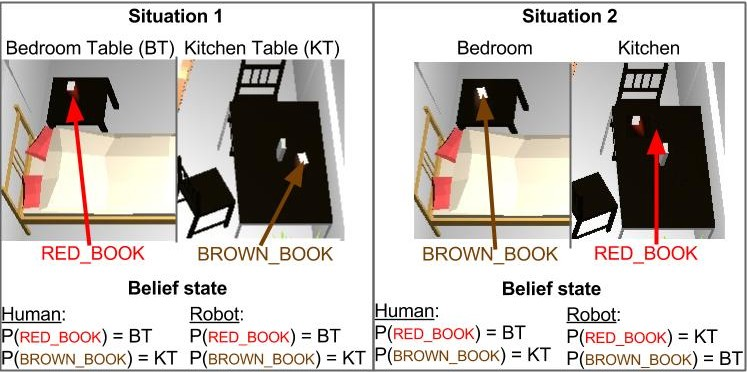
\includegraphics[width=0.89\linewidth]{./img/dbexemple.jpg} 
  \caption {Exemple où l'homme a une croyance divergente concernant l'emplacement de deux livres ayant étés interchangés.}
  \label{fig:dbexemple}
\end{figure}


Nous illustrons la prise en compte de la croyance divergente dans cette exemple avec la figure \ref{fig:overview-mardhis}. Les modifications apportées au modèle initial sont illustrées par les éléments en
orange. 
Soit la situation suivante :
l’utilisateur vient de prononcer la phrase « donne moi le livre qui est sur ma table de
chevet ». Comme le montre la figure \ref{fig:overview-mardhis}, logiquement la partition de plus grande probabilité devient celle qui modélise le but utilisateur qui consiste à vouloir lui « apporter
un livre situé sur la table de chevet ». Du point de vue du robot (ROBOT FACTS sur
la figure) ce livre est identifié de façon unique comme étant l’objet RED\_BOOK. Cependant,
du point de vue de l’utilisateur (USER FACTS sur la figure), il est également identifié
de façon unique comme étant l’objet BROWN\_BOOK. Cette situation est considérée
comme divergente et le d-status est réglé sur unique parce qu’il n’y a qu’un seul objet possible qui correspond à cette description dans le modèle de l’utilisateur et que
ce dernier est différent de celui également identifié dans la base de faits dynamiques
du robot. Dans nos travaux, le d-status ne peut prendre que les deux valeurs unique et
other, nous considérons cependant cet élément comme étant catégoriel et non binaire
car nous comptons étendre à terme le nombre des valeurs ainsi considérées (identification de différentes situations comme par exemple le fait que plusieurs objets candidats
présentent une position divergente).
En ce qui concerne la nouvelle action résumée \textit{InformDivergentBelief} introduite pour
résoudre la situation de divergence, les actes de dialogue qui lui sont associés dans
l’espace maître sont déterminés par l’intermédiaire d’heuristiques expertes. Dans cette
première version, lorsqu’un cas de divergence est détecté dans la meilleure hypothèse
d’état de dialogue, idéalement l’action prise par le système doit permettre d’informer
l’utilisateur de manière explicite de la présence et de la nature de cette divergence.
Pour ce faire, un acte de dialogue est employé pour informer l’utilisateur sur l’existence d’une divergence quant à la valeur de la position de l’objet "sujet"
de la commande. Grâce à l’émission de cet acte de dialogue l’utilisateur va pouvoir
mettre à jour ses croyances avant de poursuivre son objectif initial. Ainsi, lorsque le
système informera l’utilisateur oralement de la véritable position de l’objet en question, le modèle de croyance utilisateur sera mis à jour en fonction. Ce processus est également illustré dans la figure \ref{fig:overview-mardhis} lorsque l’action \textit{InformDivergentBelief} est sélectionnée
en tant que prochaine action du système (action maître). L’action finalement exécutée
dans l’espace maître sera : \textit{deny(object.location=bedside\_table, object.location=kitchen\_table,
object.type=book, object.color=brown)}, qui sera transformée par le NLG dans l’énoncé système suivant « le livre marron n’est plus sur la table de chevet mais sur la table de la cuisine ».
% Pour ce qui est de la politique d’interaction, nous envisageons là encore de réaliser
% un apprentissage RL en ligne de la politique. Cependant contrairement aux expériences
% réalisées dans le chapitre 4, nous considérons ici le recours à des interactions faisant
% intervenir de vrais utilisateurs (que ce soit pour l’apprentissage et les tests). Nous décrivons plus précisément les conditions expérimentales dans la section suivante.

\clearpage

\begin{sidewaysfigure}[t!]
%   \vspace{-10pt}
 \centering
 \begin{tabular}{c}
  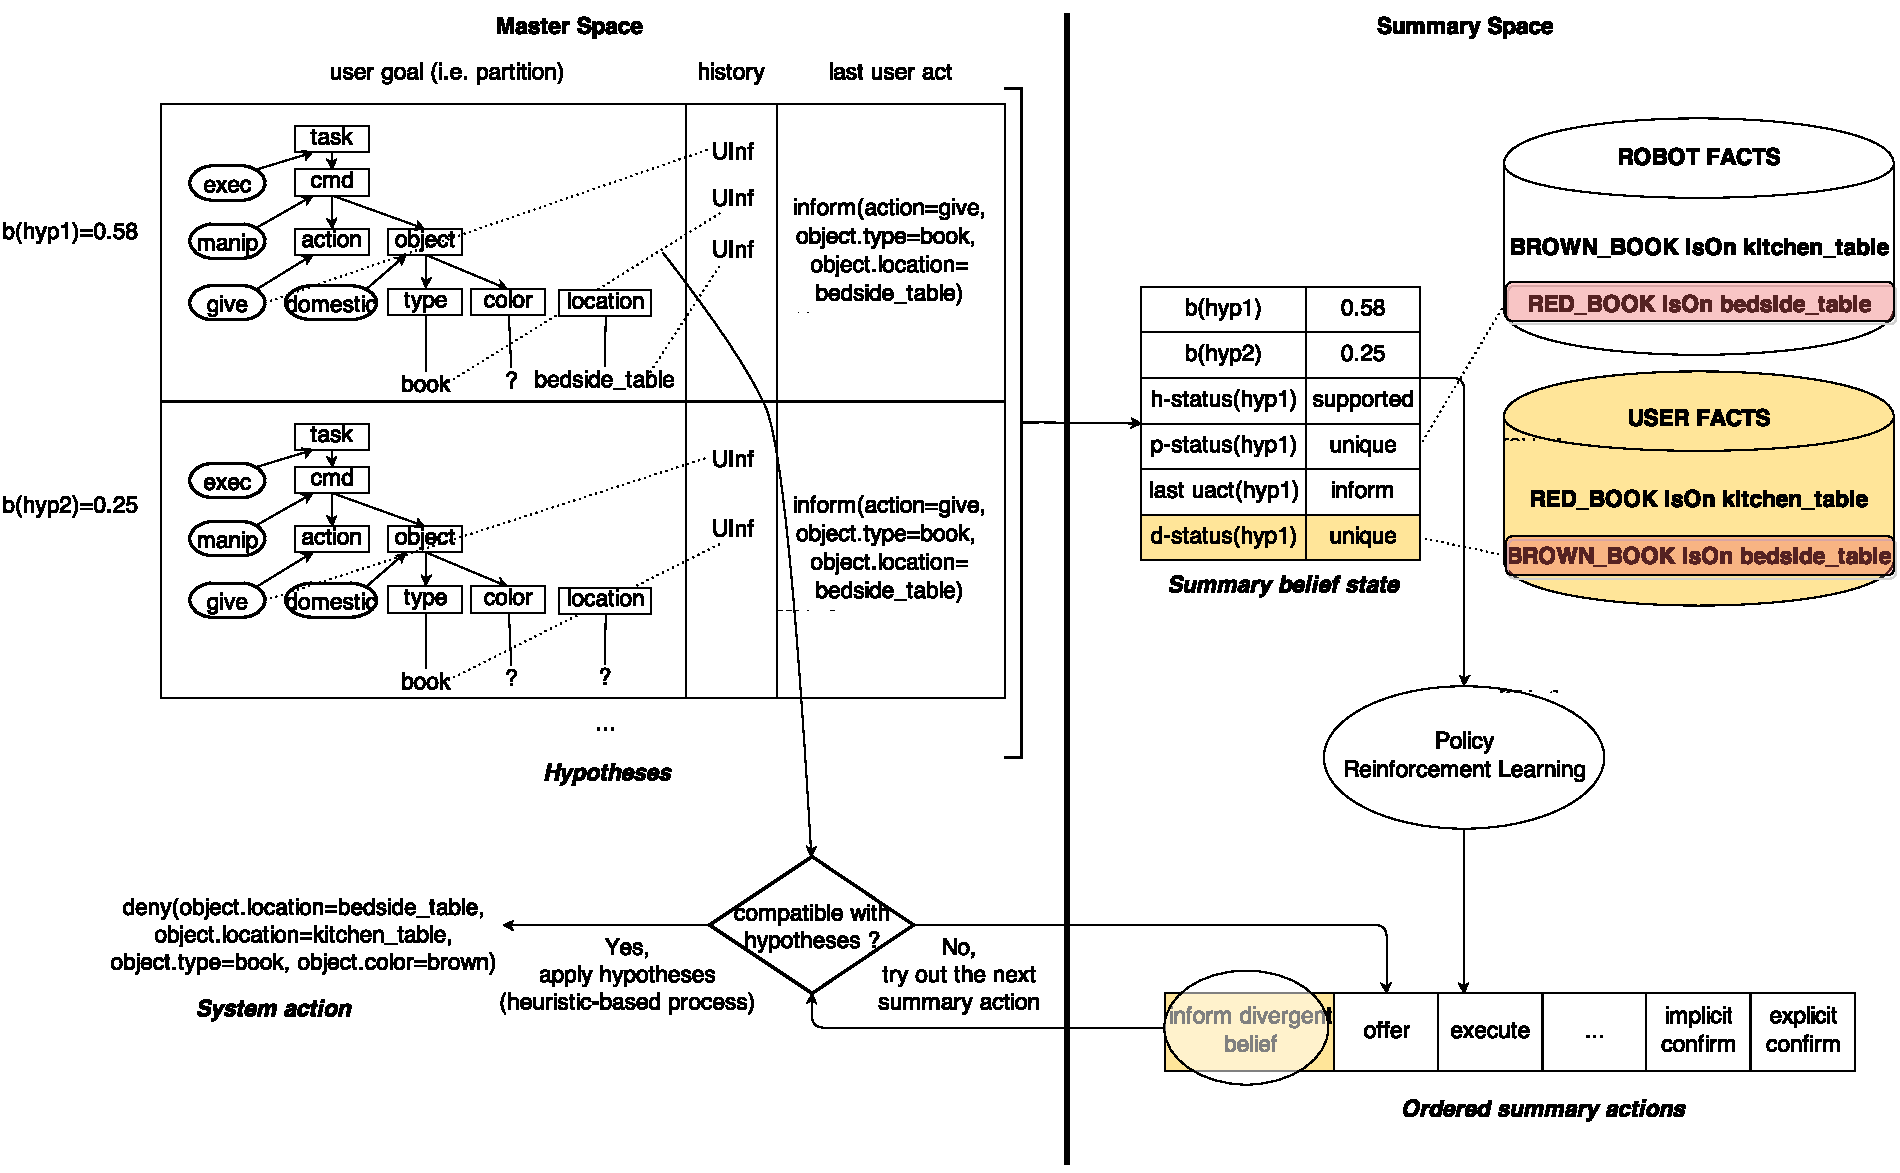
\includegraphics[width=1.0\textwidth]{img/MaRDHIS.pdf}
 \end{tabular}
 \caption{Overview of the HIS extension to take into account divergent belief.}
 \label{fig:overview-mardhis}
 %  \vspace{-10pt}
\end{sidewaysfigure}


\clearpage


% \subsection{Prise en Compte de l'État Mental}
% As mentioned earlier, an important aspect of the approach is to base our user belief state management on the POMDP framework~\cite{Kaelbling98}. It is a generalisation of the fully-observable Markov Decision Process (MDP), that was first employed to determine an optimal mapping between situations (dialogue states) and actions for the dialogue management problem in~\cite{Levin97}. We try hereafter to recall some of the principles of this approach pertaining to the modifications that will be introduced. More comprehensive descriptions should be sought in the cited papers.
% This framework maintains a probability distribution over dialogue states, called belief states, assuming the true one is unobservable. By doing so, it explicitly handles parts of the inherent uncertainty on the information conveyed inside the Dialogue Manager (DM) (e.g. error prone speech recognition and understanding processes).
% Thus, POMDP can be cast as a continuous space MDP. The latter is a tuple $<B,A,T,R, \gamma>$ 
% , where $B$ is the  belief state space (continuous), $A$ is the discrete action space, $T$ is a set of Markovian transition probabilities, $R$ is the immediate
% reward function, $R: B \times A \times B \rightarrow \Re $ and
% $\gamma \in [0,1]$ the discount factor (discounting long term
% rewards).
% The environment evolves at each time step $t$ to a belief state $b_t$ and
% the agent picks an action $a_t$ according to a policy mapping belief states to actions, $\pi: B \rightarrow A$. Then the belief state changes to $b_{t+1}$ according to the Markovian transition
% probability $b_{t+1} \sim T(.|b_t, a_t) $ and, following this, the agent received a reward $r_t =
% R(b_t, a_t, b_{t+1})$ from the environment.
% The overall problem of this continuous MDP is to derive an optimal policy maximising the reward expectation. Typically the averaged discounted sum over a potentially
% infinite horizon is used, $ \sum^{\infty}_{t=0} {\gamma^t r_t} $. Thus, for a given policy and start belief state
% $b$, this quantity is called the value function: $V^{\pi}(b) =
% E[\sum_{t\ge0}\gamma^t r_t| b_0 = b, \pi] \in \Re^B$. $V^{\ast}$ corresponds to the value function of any optimal policy
% $\pi^{\ast}$.
% The Q-function may be defined as an alternative to the value function. It adds a degree of freedom on the first
% selected action, $Q^{\pi}(b,a) = E[\sum_{t\ge0}\gamma^t r_t|b_0 = b, a_0 = a, \pi] \in \Re^{B \times A}$.
% As well as $V^{\ast}$, $Q^{\ast}$ corresponds to the
% action-value function of any optimal policy $\pi^{\ast}$. If it
% is known, an optimal policy can be directly computed by being
% greedy according to $Q^{\ast}$ ,
% $\pi^{\ast}(b) = \arg\max_a Q^{\ast}(b, a) \forall b \in B$.

% However, real-world POMDP problems are often intractable due to their dimensionality (large belief state and action spaces). Among other techniques, the HIS model~\cite{Young10} circumvents this scaling problem for dialogue management by the use of two main principles. First, it factors the dialogue state into three components: the user goal, the dialogue history and the last user act (see Figure~\ref{fig:overview-mardhis}). The possible user goals are then grouped together into \textit{partitions} on the assumption that all goals from the same partition are equally probable. These partitions are built using the dependencies defined in a domain-specific ontology and the information extracted all along the dialogue from both the user and the system communicative acts. In the standard HIS model, each partition is linked to matching database entities based on its static and dynamic properties that corresponds to the current state of the world (e.g. colour of an object vs spatial relations like \textit{isOn}).
% The combination of a partition, the associated dialogue history, which corresponds here to a finite state machine that keeps track of the grounding status for each convoyed piece of information (e.g. informed or grounded by the user), and a possible last user action forms a dialogue state hypothesis. A probability distribution $b(hyp)$ over the most likely hypotheses is maintained during the dialogue and this distribution constitutes the POMDP's belief state.
% Second, HIS maps both the belief space (hypotheses) and the action space into a much reduced summary space where RL algorithms are tractable.
% The summary state space is the compound of two continuous and three discrete values. Continuous values are the probabilities of the two-first hypotheses $b(hyp1)$ and $b(hyp2)$ while the discrete ones, extracted from the top hypothesis, are the type of the last user act (noted \textit{last\ uact}), a partition status (noted \textit{p-status}) database matching status related to the corresponding goal and a history status (noted \textit{h-status}).
% Likewise system dialogue acts are simplified in a dozen of summary actions like \textit{offer}, \textit{execute}, \textit{explicit-confirm} and \textit{request}. Once the summary actions are ordered by their $Q(b,a)$ scores in descending order by the policy, an handcrafted process checks if the best scored action is compatible with the current set of hypotheses (e.g. for the \textit{confirm} summary act this compatibility test consists in checking if there is something to confirm in the top hypothesis). If they are compatible, an heuristic-based method maps this action back to the master space as the next system response. If not, the process is pursued using the next best scored summary action until a possible action is found.

%> MaRDHIS model
% \begin{figure}[t!]
%    \vspace{-10pt}
%  \centering
%  \begin{tabular}{c}
%   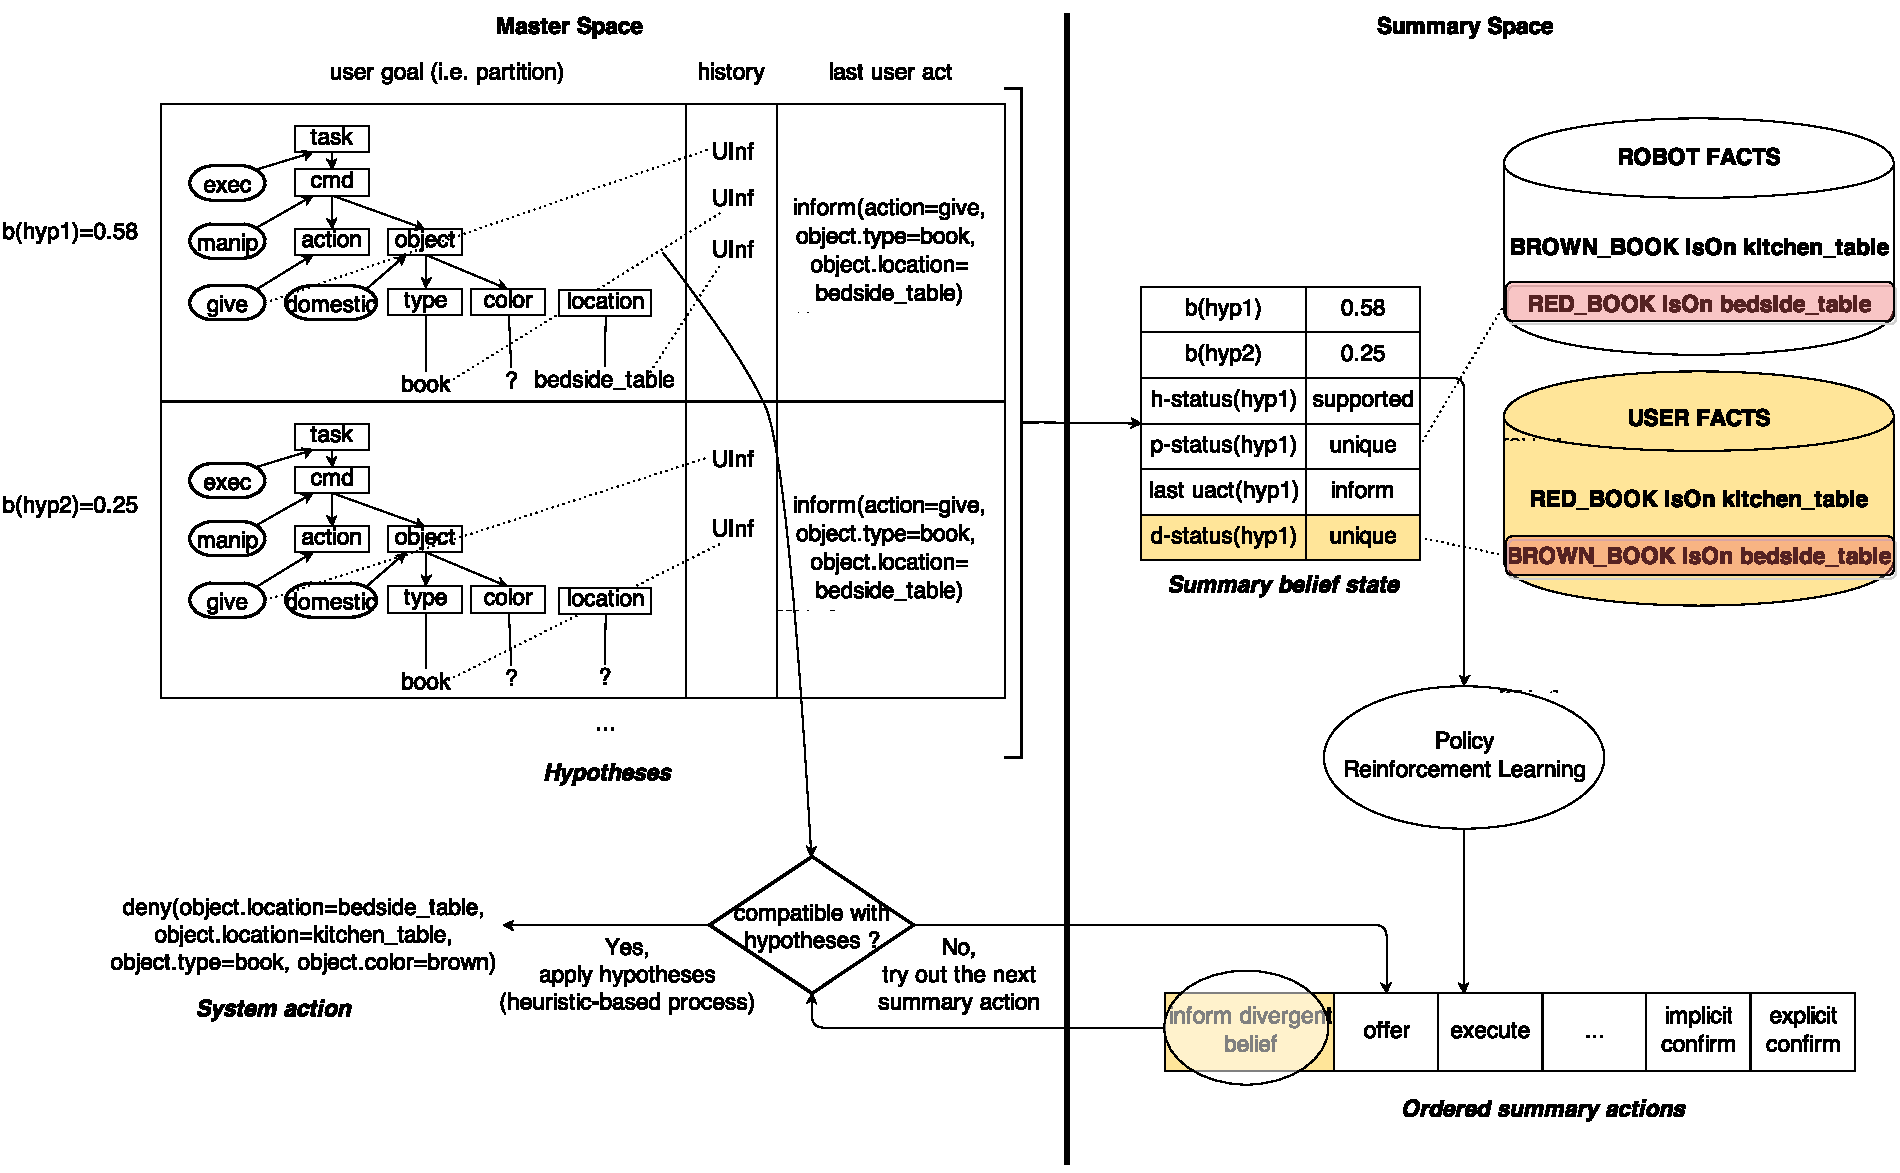
\includegraphics[width=0.98\textwidth]{img/MaRDHIS.pdf}
%  \end{tabular}
%  \caption{Overview of the HIS extension to take into account divergent belief.}
%  \label{fig:overview-mardhis}
%    \vspace{-10pt}
% \end{figure}

% Reviewer 3 => First, I am wondering whether a case when a user has a false belief can be (and needs to be) separately treated with a case with noises in the communicative channel.
% MANU> perso je trouve que le paragrapthe ci-dessous y reponds
%
% Greg> Proposition de simplification:
% GREG> Je trouve que la phrase suivante est "missleading". Notamment le untill she is notified, parceque au final ca peut etre compris comme etant justement une reaction appropriee.
%Indeed, according to her mental belief the user may still want to pursue her goal with an erroneous statement until she is notified, or discovers by herself, that it does not correspond to the true current state of the world. 
% Old
% If the standard HIS framework can properly handle misunderstandings due to noise in the communicative channel, it offers no appropriate mechanism for such a case where the user has a false belief about the state of the world which should impact negatively its communicative acts. Indeed, according to her mental belief the user may still want to pursue her goal with an erroneous statement until she is notified, or discovers by herself, that it does not correspond to the true current state of the world.
% New
% The standard HIS framework can properly handle misunderstandings due to noise in the communicative channel.
% However, misunderstandings can also be introduced in cases where the user has false beliefs, impacting negatively her communicative acts. HIS has no dedicated mechanism to deal with such a situation and so it should react as in front of a %classical uncertainty by keeping requiring the user some confirmations of hypotheses until the request can match the reality, although it could have be resolved since the first turn. 
% classical uncertainty by asking the user to confirm  hypotheses until the request can match the reality, although it could have be resolved since the first turn. 
% Therefore having an appropriate mechanism should improve the quality and efficiency of the dialogue, preventing user to pursue her goal with an erroneous statement.

% So, as illustrated in Figure~\ref{fig:overview-mardhis} and highlighted with the orange items, we propose to extend the summary belief state with an additional status, the
% \textit{divergent belief} status (noted \textit{d-status}), and an additional summary action, \textit{inform divergent belief}.
% % GREG> I think it's hard here to understand what we mean by user facts and how it is different from partition.
% % so I added "(from user's belief model)"
% The \textit{d-status} is employed to trigger the presence of false belief situations by matching the top partition with user facts compiled by the system (see Sec.~\ref{sec:knowledge}) and as such trying to highlight some divergences between the user and the robot points of view. 
% %>>>BEGIN MODIF
% %Reviewer 3 => Are the user facts in Figure 2 maintained as an internal state of the system?  If yes, how is it updated or detected?
% %NEW>
% %****
% Both the user and the robot facts (from the belief models, not to be mistaken with the belief state related to the dialogue representation) are considered as part of the dynamic knowledge resource and are maintained independently of the internal state of the system with the techniques described in Sec.~\ref{sec:knowledge}.
% %>>>END MODIF
% Here we can observe in Figure~\ref{fig:overview-mardhis} that the top partition is about a book located on the bedside table. In the robot model of the world (i.e. robot facts) this book is identified as a unique entity, RED\_BOOK, and \textit{p-status} is set to \textit{unique} accordingly. However, in the user model it is identified as BROWN\_BOOK. This situation can be considered as divergent and \textit{p-status} is set to \textit{unique} too because there is one possible object that corresponds to that description in the user model. 
% %>>>BEGIN MODIF
% %WHY>
% %***
% %Reviewer 3 => The d-status is also unclear although it should be clearly defined. What values it has other than "unique"?  
% %NEW>
% %***
% In this preliminary study \textit{d-status} can only be \textit{unique} or \textit{non-unique}. Further studies may consider more complex cases.
% %>>>END MODIF
% %
% The new summary action is employed for appropriate resolution and removal of the divergence.
% The (real) communicative acts associated to this (generic) action relies on expert design. In this first version, if this action is compatible with the current hypotheses and thus picked up by the system, it explicitly informs the user of the presence and the nature of the divergence. To do so, the system uses a \textit{deny} dialogue act to inform the user about the existence of a divergent point of view and let the user agree on the updated information. 
% % GREG> Maybe explain here that we don't manage the situation when robot is wrong
% % review: It would be good to discuss other issues related to false beliefs
% Consequently, the user may pursue its original goal with the correct property instead of the obsolete one. This process is also illustrated in Figure~\ref{fig:overview-mardhis} when the \textit{inform divergent belief} action is mapped back to the master space.

%%%%%%%%%%%%%%%%%%%%%%%%%%%%%%%%%%%%%%%%%%%%%%%%%%%%%%%%%%%%%%%%%%q


\subsection{Restitution Multimodale}
Quatre modules sont actuellement responsables
des sorties du système.
Le module de fission a en charge
le processus de traduction des décisions abstraites (actes de dialogue haut niveau) du système vers des actions verbales et non-verbales (déplacement, prise de position).
Pour l’instant, ce module est basé sur la définition d’un ensemble de règles prenant
en compte la nature de la décision du système et le contexte courant (base de faits des
différents agents). La solution retenue considère également les flux de sorties comme
parallèle (pas de synchronisation fine entre gestes et paroles).
Pour la restitution vocale du système, deux modules interviennent, NLG et TTS. Le
premier s’appuie sur des patrons lexicaux similaires à ceux présentés dans section 2.1.1
(voir tableau 2.1.1), le second module a quant à lui été spécialement implémenté par
notre partenaire ACAPELA Group dans le cadre du projet MaRDi. Son originalité réside
dans le fait qu’il repose sur des mécanismes d’interpolations de modèles pour élargir la
richesse expressive de la voix employée tout en offrant un contrôle continu pour moduler
dynamiquement la voix au cours de la synthèse d’un même énoncé (Astrinaki et al.,
2012). Dans sa version actuelle nous pouvons donc jouer sur trois paramètres simultanément,
à savoir le style de voix (portée, chuchotée ou normale), l’émotion transmise
(ton joyeux, triste ou normal) et la vitesse d’élocution (rapide, lente, normale).
Selon la nature de l’acte de dialogue sélectionné par le système et le contexte interactif,
le module de fission va donc attribuer une étiquette sur l’acte vocal pour que le
module TTS puisse faire une synthèse expressive de la phrase générée par le NLG. Par
exemple, si l’utilisateur et le robot ne sont pas dans la même pièce le module de fission
va attribuer l’étiquette indiquant qu’il va falloir que le robot parle plus fort (avec
une voix portée), ou encore si le système informe l’utilisateur qu’il ne peut pas réaliser
l’action (par exemple si l’objet est hors de porté pour lui) alors il pourra faire jouer une
synthèse vocale employant une voix triste.
En ce qui concerne la gestuelle et les actions physiques du robot, elles vont se
faire grâce à l’utilisation d’une interface abstraite, NVBP/MC pour Non-Verbal Behaviour
Planner and Motor Control en anglais. De par son haut niveau d’abstraction, cette
dernière nous permet de faire tourner le système de façon similaire que ce soit sur la véritable
plateforme robotique ou sur l’outil de simulation 3D décrit dans la section 6.3.2.
Dans notre scénario, deux situations distinctes vont impliquer des mouvements de la
part du robot. La première est liée à l’exécution de la commande de déplacement d’objet
utilisateur, cette dernière intervient toujours en fin d’interaction car l’exécution d’une
commande erronée est également synonyme d’échec dans notre scénario. La seconde
situation consiste en l’exploration de l’environnement. Elle est utilisée pour acquérir
des faits symboliques sur des zones non explorées (par exemple aller voir ce qu’il y a
sur la table de la cuisine).
Le module de fission utilise l’interface abstraite pour transmettre les commandes
haut niveau, par exemple move(BLACK\_TAPE, kitchen\_table,bedroom\_bedsidetable) ou explore(
kitchen\_table). Dans le cas où la plateforme robotique est employée, ces buts vont
être transmis à un superviseur qui va dans un premier temps planifier les actions devant
être exécutées par l’intermédiaire d’HATP (pour Human Aware Task Planner) (Alami
et al., 2006), puis procéder à leur exécution d’après le plan ainsi établi. En simulation,
l’exécution de ces commandes haut niveau est grandement simplifiée. En effet, elles
sont traduites en séquence d’actions élémentaires selon des patrons prédéfinis dont nous donnerons quelques exemples dans la section 6.3.2.




\section{Implémentation Dans un Simulateur Robotique}

\subsection{Motivation}
Les systèmes de simulation sont très utilisés en robotique. Ils permettent aux roboticiens d'évaluer et valider leur travaux au niveau d'abstraction souhaité. De cette manière, les projets reposant sur des calculs de haut niveau (interaction, dialogue, supervision) peuvent utiliser un simulateur pour abstraire les niveaux inférieurs (navigation, traitement d'image, manipulation) et eviter que les problèmes qui leur sont liés interferent durant l'intéraction.

Pour le projet MaRDi, le simulateur est également utile pour partager un même environnement et une même configuration expérimentale entre les différents partenaires. Il est cependant nécéssaire que le simulateur soit adapté à l'intéraction homme-robot. 
En terme de simulation, deux solutions sont possible pour ajouter l'homme à la boucle: 1) en modelisant et implémentant leur comportements et actions, et 2) en utilisant la téléopération pour controler les avatars humains.

La première solution présente l'avantage de l'automatisation et ne demande aucune manipulation manuelle. Cette solution est donc moins couteuse en temps et plus facile à mettre en place. Cependant, selon les caractéristiques humaines requises, il est potentiellement extrèmement complexe d'avoir un modèle de comportement humain réaliste. Les humains sont des entités complexes avec des réactions et comportements quasi impossible de synthétiser de manière satisfaisante. Cette solution est en général retenue pour les études qui n'impliquent pas les comportements humains les plus complexes, comme la navigation ou la manipulation.

Dans la seconde solution, un homme téléopère un avatar virtuel. La simulation est donc plus complexe à établir car elle nécéssite de monopoliser un humain. Cependant, l'avatar du simulateur aura un comportement beaucoup plus réaliste. Pour ce faire, l'environement doit avoir un rendu visuel réaliste et le contrôle de l'avatar doit être suffisamment intuitif.

D'autres projets de dialogue situé homme robot reposent sur une étude dans un simulateur. Par exemple pour un scénario de Pick-Place-Carry (Prendre-Placer-Transporter) \cite{Lucignano13}, de robot barman \cite{stiefelhagen07} ou de navigation dans un environnemnt virtuel \cite{byron06}. Cependant, peu de travaux considèrent l'environnement de simulation comme moyen pour l'aquisition du corpus de dialogue situé ou comme moyen de tester l'apprentissage de politique en ligne.
%Indeed, most of the previous works in situated dialogue for HRI resorted to a preliminary Wizard-of-Oz (WoZ) experiment, where a human remotely operates the robot %, and then, used the collected data to train both a user simulator and an error model to pursue the dialogue policy learning without the use of any new real interactions
%
En effet, la plupart repose sur des expériences en magicien d'Oz \cite{prommer06,stiefelhagen07,rieser08}. 
%However, the WoZ technique is both time consuming and an expensive method.



\subsection{Choix du Simulateur}

In the robotic field, many simulators are available. We can name the Player/Stage/Gazebo suite~\cite{psg-1232}, the integrated simulation platform OpenHRP \cite{nakaoka|iros07}, the cross-platform software architecture OpenRAVE \cite{diankov_thesis} or even the commercial simulator V-REP \cite{Freese2010}. However, only a few of them are very well suited to HRI. They generally limit human agent behaviours to relatively simple motions and interaction capacities which is one of the reasons why HRI simulations so far have been carried out in \emph{tele-operation} settings, where only the robot and the environment, but not the human agent, are actually simulated. Robotic simulators USARSim \cite{Lewis07usarsim} and MORSE \cite{morse_simpar_2012,simparmorse2014} are both used in dozens of HRI studies due to their explicit support for controlling a human agent. However, the latter has several specific advantages that motivated our choice. 

% open-source / active communauty / middleware supports 
MORSE is an open-source simulator, with a very active community, that was developed specifically for robotic simulation. It supports a wide range of middleware (e.g. ROS, YARP, pocolibs) as well as reliable implementations of realistic sensors and actuators which ease the integration on real robotic platforms afterwards.
% Sensors / actuators with different level of abstraction
%OLD>
%The fact that virtual robots can interact with the virtual environment, not only through realistic sensors and actuators, but also by using higher level of abstraction makes it an adaptable tool for diverse research topics.
%In this way, HRI simulation scenario can avoid to run low level sensors along with their related computation stack but can directly process high level data from unrealistic sensor. 
%NEW> 
Moreover, MORSE offers an adaptable simulation setup by allowing virtual robots to interact with the virtual environment through both realistic sensors/actuators and higher level ones. Thereby, roboticists can control the related computation cost of low level data processing by exploiting high level outputs from unrealistic components. 
%
For example, MORSE provides both a vision camera and a
semantic camera sensor. While the first camera provides a rough image (i.e. raw pixels) as output, the second one
gives directly the names of the perceived objects and their positions in the scene. 
%OLD> The latter sensor avoids users to perform object recognition and localization process when working on higher level issues
%and still process same data while using a smaller computing environment.
%NEW>
The latter sensor avoids practitioners to perform object recognition and localization processes when focusing on higher level issues.

% Realistic rendering
Furthermore, MORSE relies on the Blender Game Engine,
a real-time 3D runtime integrated to the open-source Blender
modelling toolkit, for both advanced 3D (OpenGL shader) and
physics simulation (based on the BULLET physics engine).
This setup allows realistic rendering of complex environment and provides an immersive graphical user interface, which is a required feature %for immersive control of a human avatar.
for HRI modelling. 

% Human avatar controls
In MORSE, the human avatar can be controlled by a human operator or directly through external scripts as any other robot.  

\begin{figure}[ht!]
 \centering
 \begin{tabular}{cc}
  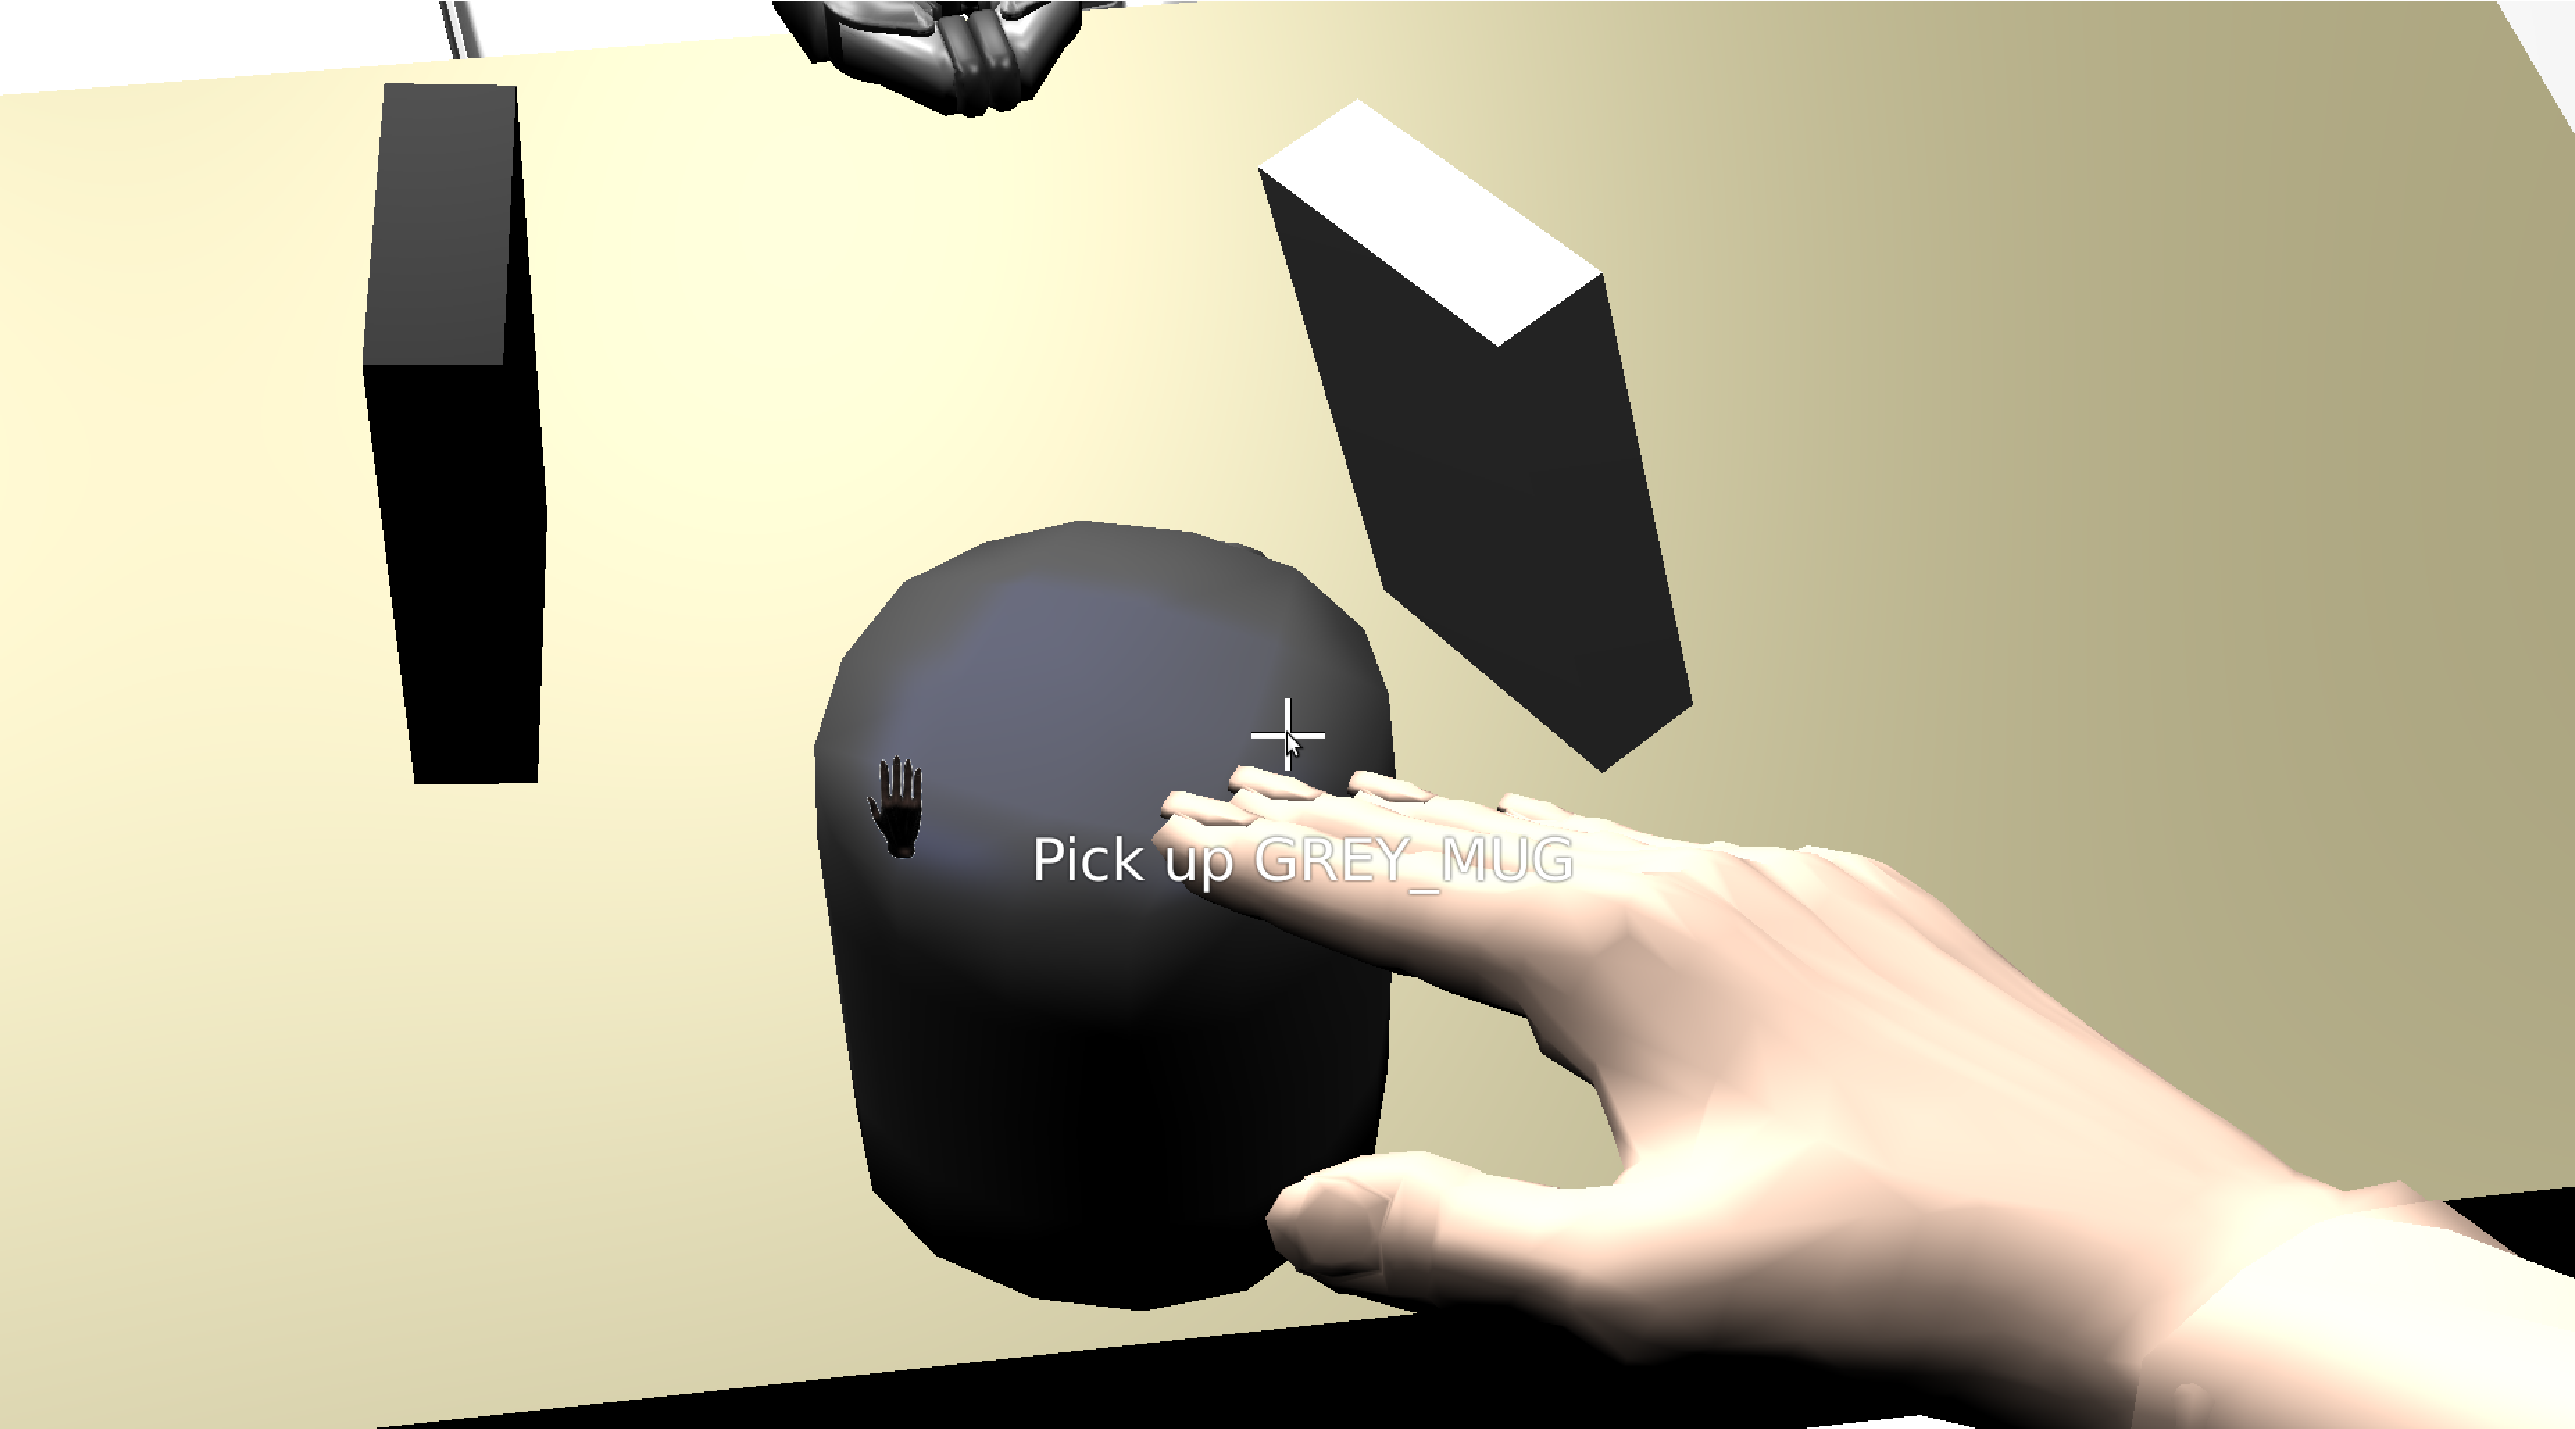
\includegraphics[width=0.475\textwidth]{img/Screenshot_from_2014-04-29_14_02_14.png} &
  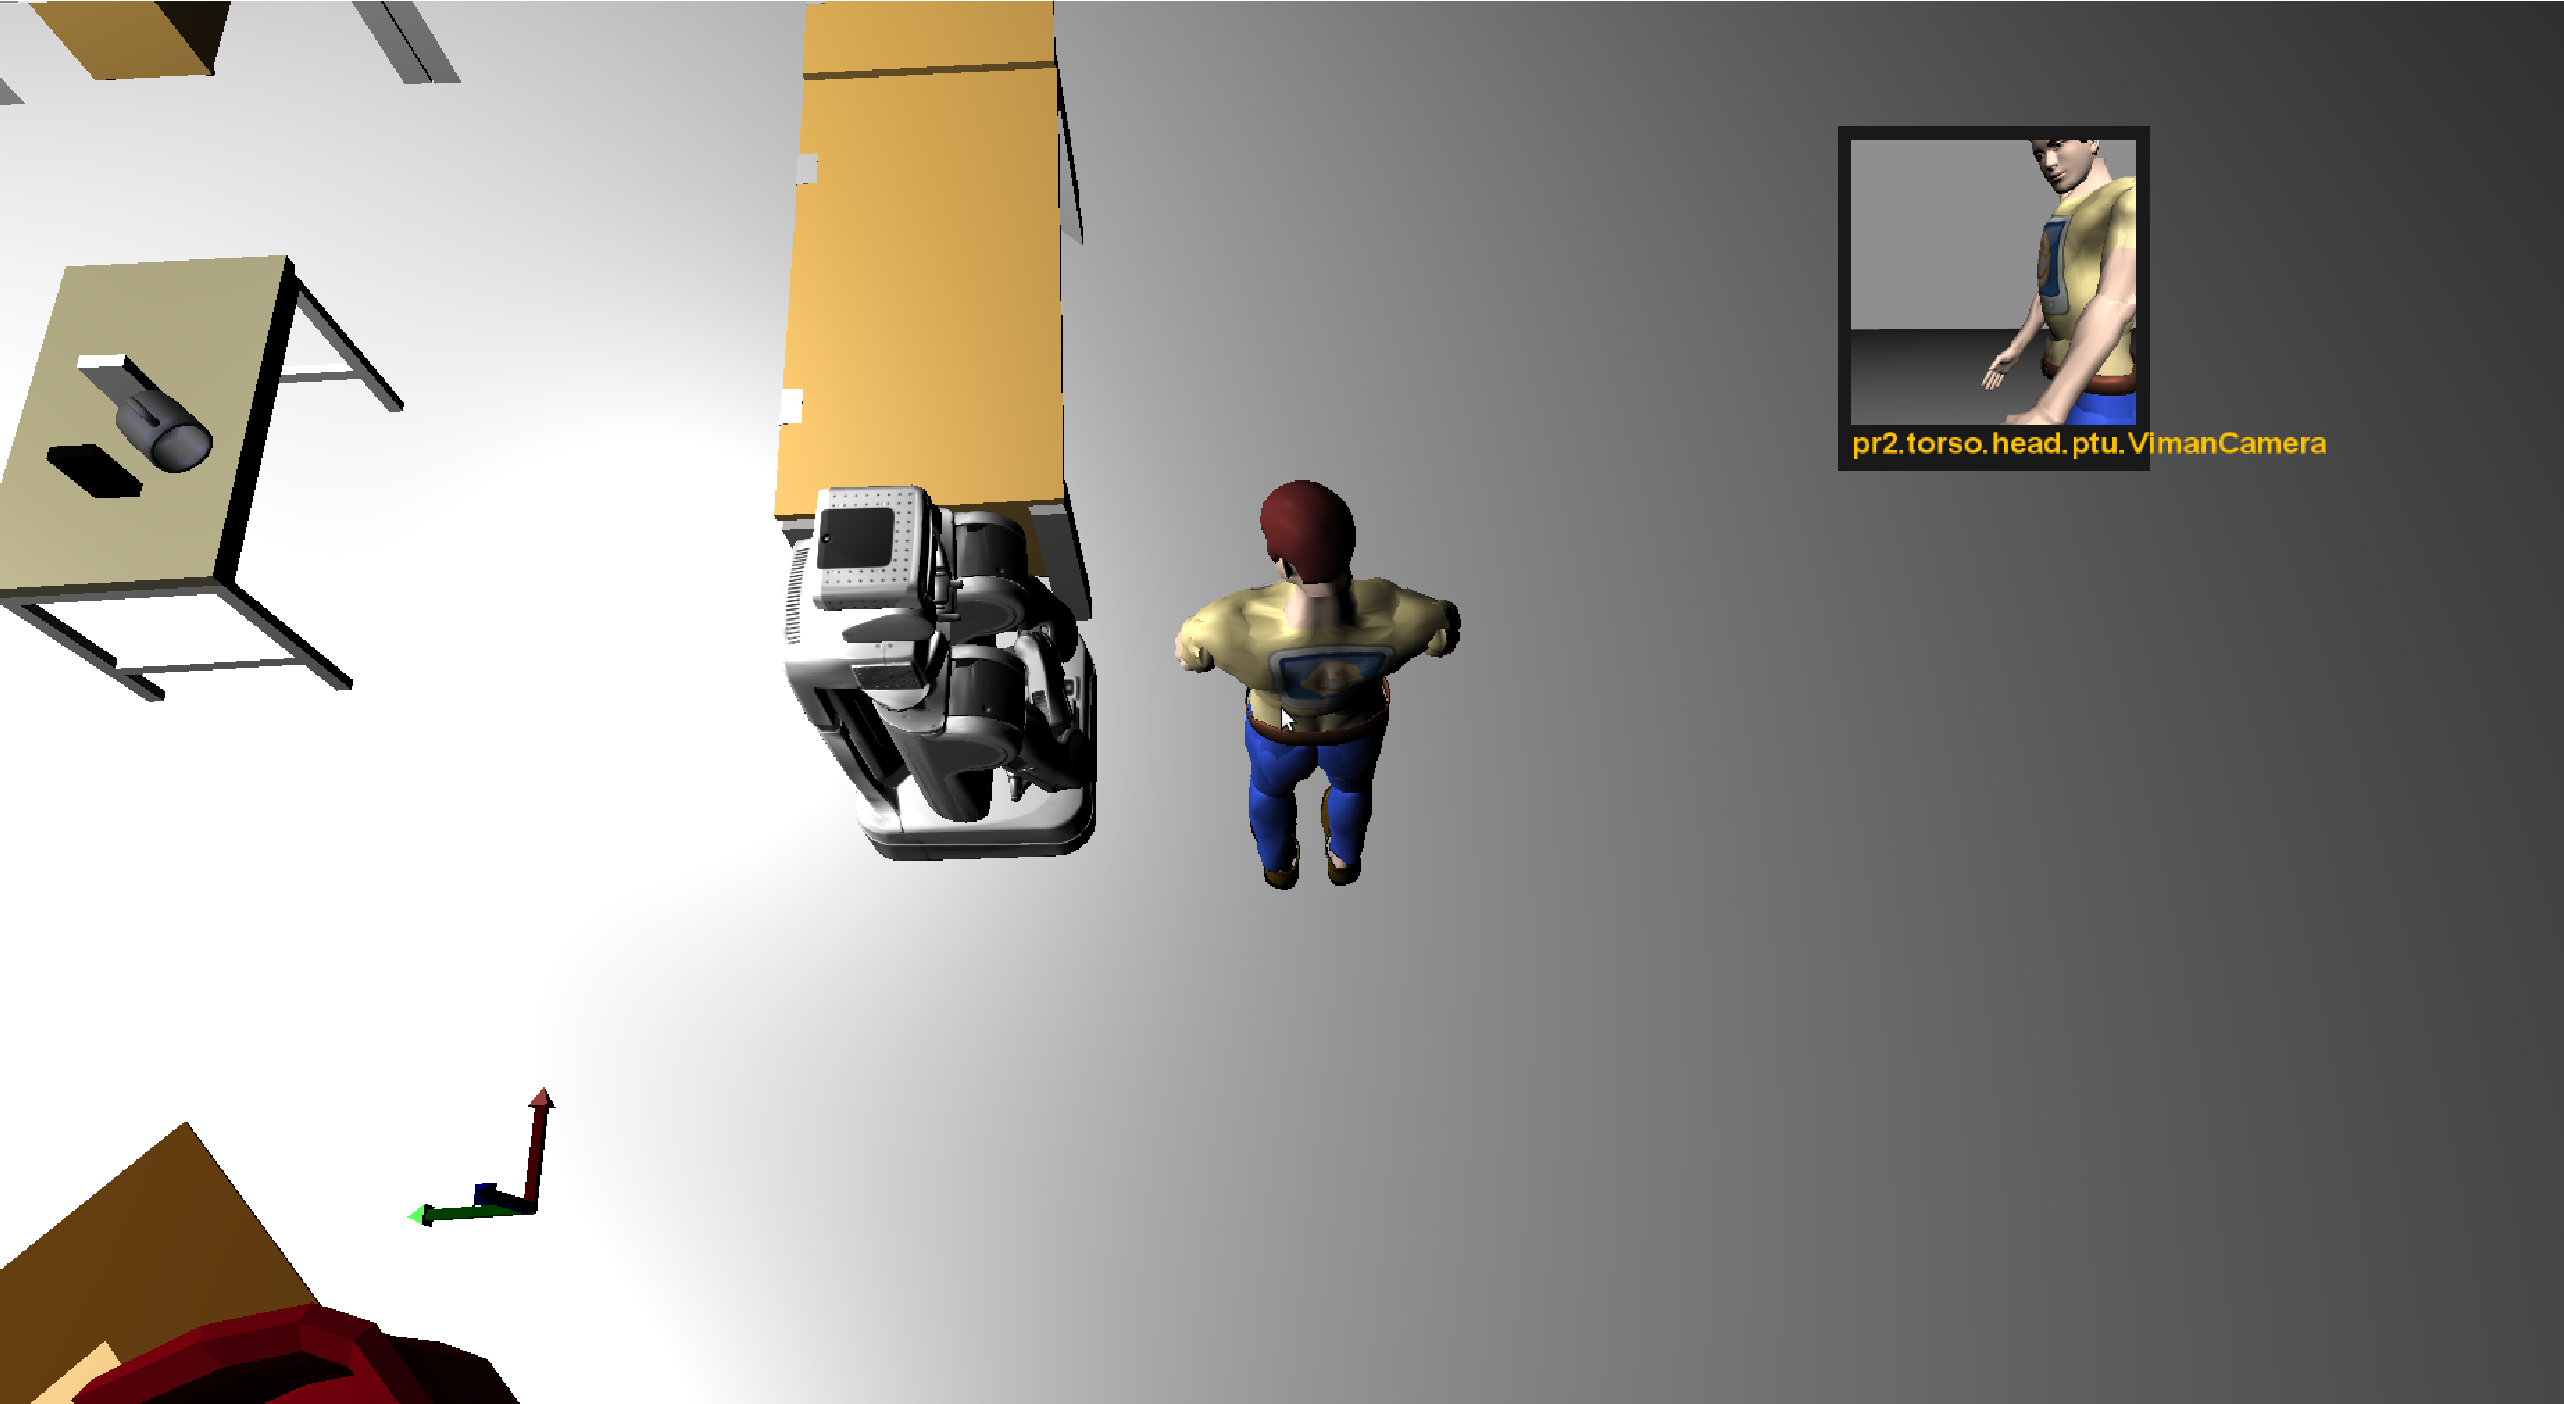
\includegraphics[width=0.475\textwidth]{img/Screenshot_from_2014-04-29_14_21_24.png}
 \end{tabular}
 \caption{Human avatar grabbing an object controlled by an operator (left image) and human in 3rd person perspective (right image).}
 \label{fig:human_morse}
   \vspace{-3pt}
 \end{figure}
%In the first case, the operator controls the virtual human in an immersive way (i.e. first-person-shooter style). 
%Displacement, gaze and interactions with the environment such as object manipulation can be controlled by the operator. 
%These features are highly appreciated for enabling realistic behaviours of the simulated human.
In the first case, the operator controls the virtual human in an immersive way (see Figure~\ref{fig:human_morse}) in terms of displacement, gaze, and interactions on the environment, such as object manipulation (e.g. grasp/released an object).
To go even further in realistic human incorporation in the simulator, 
a motion capture actuator allows to control the human avatar directly 
by using an external device. So, a Kinect sensor collects human gestures and sends the posture data to %the actuator that will 
move the human avatar accordingly.
%For the operator to manipulate an object, a Nintendo wiimote can also be used to control this action.
Furthermore, a Nintendo wiimote can jointly be used to manage its action (e.g. grasp/released an object).

In the second case, the avatar is programmatically controlled by using standard MORSE actuators. As an example, it is possible to use a waypoint actuator on the human to define a path he has to follow.


%%%%%%%%%%%%%%%%%%%%%%%%%%%%%%%%%%%%%%%%%%%%%%%%%%%
\subsection{Simulation de l'interaction}
In our scenario, a disabled human is in her apartment and has a robot to assist her to perform everyday life chores.
The goal is to make the robot understand, by reasoning on human speech, gestures and the environment, human's requests concerning objects. Objects are limited here to graspable items such as books, DVDs and mugs, that have diverse colors and a unique identifier.

The PR2 robot is used in the simulator as it is our real platform at LAAS-CNRS. PR2 is already present in MORSE models, making it directly usable. We add a symbolic camera (MORSE semantic camera) sensor to the standard model so that it can perform object recognition and also a teleport actuator to move it to a designated position (while saving the time of the true displacement). We also add a human avatar with first person representation to have realistic inputs of speech and behaviour of human users. We use a virtual model of the physical environment in which the real robot will be tested (see Figure~\ref{fig:env}).
% TODO take a screenshot of env with objects

\begin{figure}[ht!]
 \centering
 \begin{tabular}{cc}
  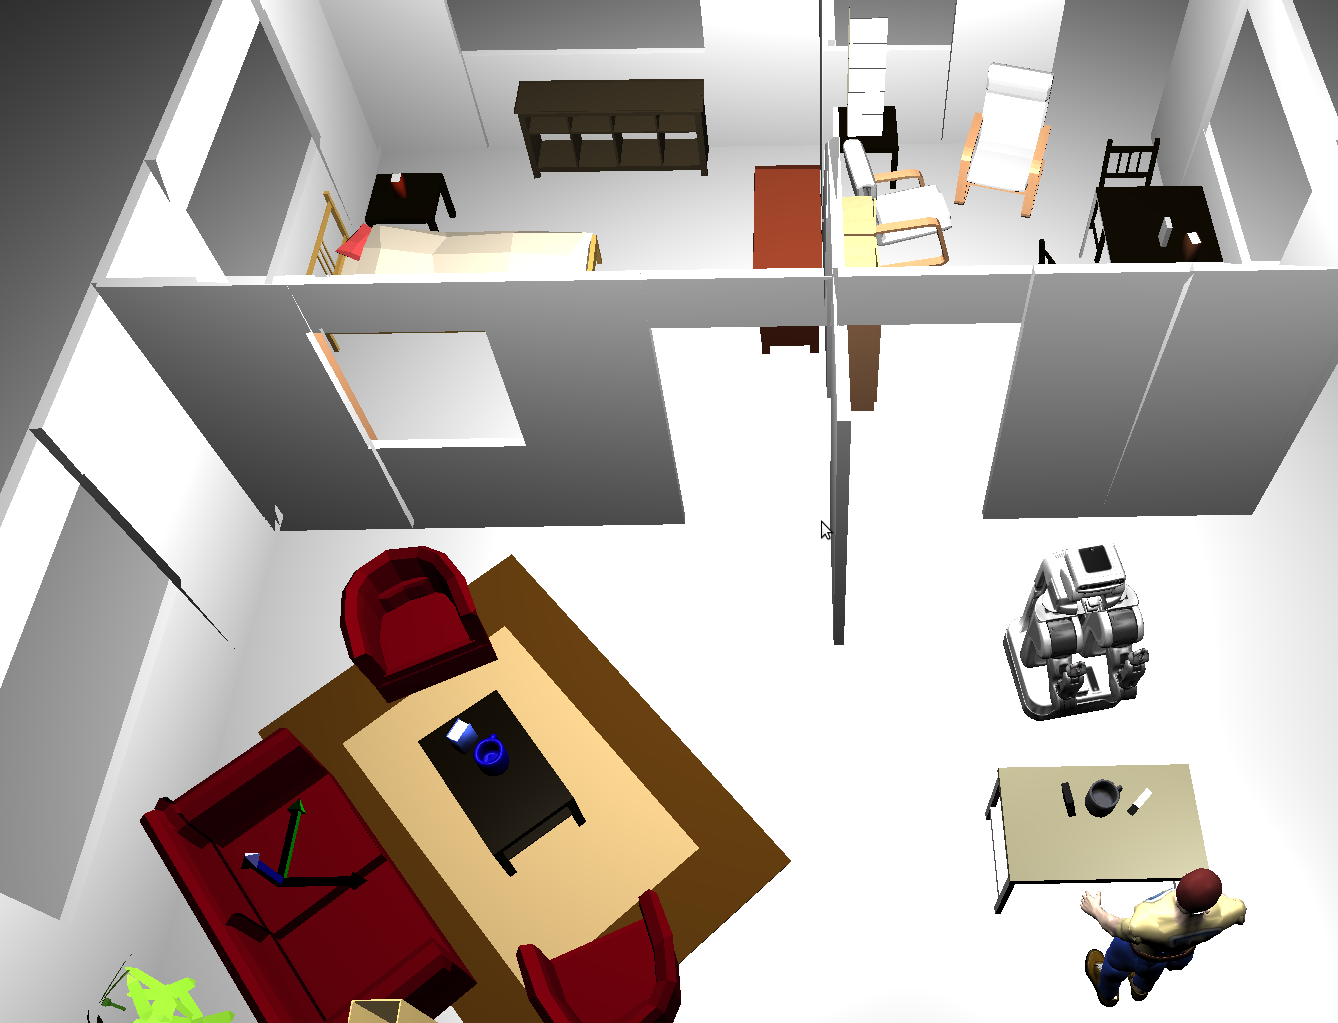
\includegraphics[width=0.6\textwidth]{img/LAASMORSE.png}
 \end{tabular}
 \caption{Scenario environment in MORSE}
 \label{fig:env}
 \end{figure}
 
At the start of the simulation, a script randomly positions objects in predefined areas
(such as over kitchen table, living-room table, bedroom shelf etc.), called \textit{manipulation areas}. This allows us to use different environment configurations without changing the initialization files (MORSE builder script).

% -> Detail how we build our scene according to our scenario
% -> Detail Morse tools we use in our scenario and how they work and fit our needs: Semantic camera, teleport, grasp


%-----------------------------------------------%
\subsection{Actions library}
\label{section:actions}
%-> Why we need these actions?
%   -> Simulation more interactive and realistic
%    -> Objective fulfillment evaluation according to robot action (users satisfaction)
To get a more interactive and realistic simulation and also for the user to
evaluate the fulfilment of her request (e.g. does the robot bring the appropriate object),
we have developed a library of high-level and abstract actions that the robot will be able to perform.

The list of abstract actions is as followed:
\begin{itemize}

% Move robot to manipulation area
\item To explore the environment and bring an object to the human, the robot needs to be able to move to manipulation areas. To do so, we use the teleport actuator of MORSE. This actuator moves instantaneously the robot to a given place. We define a script function to move the robot to each manipulation area that has been defined. In this way the robot can go to each position to pick objects or explore an area to get some contextual information.

% Explore an area
\item The robot is able to scan a manipulation area. To make this action possible a symbolic camera is added to the robot on its head. We then move the head sequentially to scan the environment.

% Grab object
\item The robot has to grab an object. To perform this action the grasp service of the PR2 is used. We specify the name of the object it has to grab and if the object is close to robot's hand it will be attached to it. In a similar way, we added a function to drop an object that takes as parameter the manipulation area where it should be dropped to. The robot will drop the object on top of the corresponding furniture.

% Give object
\item The last action is giving the object to the human. It consists in moving the robot to the human position and deploying the arm of the robot toward the human to give her the object. We simply use the robot armature actuator to control the robot's arm.
\end{itemize}



\subsection{Expérimentation et résultats}
In this "proof of concept" study we chose to deal with a limited expert panel, composed of 6 subjects (2 females and 4 males of around 25 years old), in order to focus on the capacity of the system to learn from scratch using a limited set of interactions. The advantage is that the collected data sufficiently explore the state and action spaces during the online learning to be exploited in offline learning (using batch samples).

At the beginning of each dialogue, a specific goal (here a command) is randomly generated taking into account the simulated environment settings and the current interaction history in order to select a possible command. For example, "You want the robot to give you the white book on the kitchen table". No experimenter has any idea of the chosen configuration of the system with which he is interacting. So, we basically compare a hand-crafted expert dialogue policy (noted HDC) to a learned one (noted LEARNED). The latter was trained using a small set of expert users which first performed $60$ dialogues in an online learning setting.

In the complete multimodal architecture, each interaction takes from $7$ to $10$ minutes to complete (objects detection, robot movements, etc.).  So, without loss of generality, a practical workaround to speed-up the testing process consisted in using a fixed representation of the scene (a screenshot from the human point of view) and a web-based multimodal GUI instead of the full simulation setup.  Overall, $84$ dialogues for both the two proposed systems were recorded with $6$ distinct subjects. At the end of each interaction users evaluated the system in terms of task completion. The learned policy were configured to act greedily according to the value function. Results are those gathered in test condition where exploration is not allowed. All the dialogues were  recorded both in terms of audio and various kinds of meta-information (e.g. ASR N-Best list, dialogue manager detected gestures and related timestamps, etc.) but also high level annotations (e.g. environment settings, pursued goal, task success). As an illustration, a short interaction, translated from French, is given in Table~\ref{table:hri-example}.

\begin{table}
\centering
\small
\begin{tabular}{|c|c|l|}
  \hline
  \multirow{3}{*}{R1} & DA & hello() \\
    & NLG/TTS & Can I help you ?\\
    \hline
  \multirow{3}{*}{U1} & ASR & Can you put the book in my bedroom? \\
  	& SLU & inform(action=move,desc=in,room=bedroom)\\
    \hline
  \multirow{3}{*}{R2} & DA & confreq(type=book,position) \\
    & NLG/TTS & Sorry but where is the book you are talking about?\\
    \hline
  \multirow{3}{*}{U3} & ASR & I am talking about this one \\
  	& SLU & inform(idobj=?)\\
    & GRU & pointsAt BLUE\_BOOK 1395848705.31\\
   \hline
    \multirow{4}{*}{R3} & & execute(action=move,destination=bedroom\_bedsidetable,\\
     & DA & idobj=BLUE\_BOOK,position=livingroom\_table,type=book,\\
    & &color=blue) \\
    & NVBP/MC & move(BLUE\_BOOK,livingroom\_table,bedroom\_bedsidetable)\\
    & NLG/TTS & Ok, I will put the blue book on your bedside table\\
    \hline
\end{tabular}
 \caption{Example of a multimodal dialogue.}
 \label{table:hri-example}
 \vspace{-20pt}
 \end{table}
 
The results obtained are $14.3$ for the HDC method and $17.6$ for the LEARNED one. These results are given in terms of mean discounted cumulative rewards~\cite{Sutton98}. According to the reward function definition, this metric expresses in a single real value the two variables of improvement, namely the success rate (accuracy) and the number of turns until dialogue end (time efficiency). So, here the HDC policy manages the dialogue with $86\%$ of success rate in an average of $4.8$ turns against respectively $93\%$ and $2.9$ turns for the LEARNED one.  The difference observed between the two methods can be mainly explained by a more accurate and less frequent usage of request of confirmation as well as an expected more fined-grained uncertainty management for the LEARNED method. Thus, these results clearly both demonstrates the ability of the overall architecture (simulation software + multimodal dialogue system) to learn an efficient dialogue policy using few dialogue examples and shows the interest of considering RL methods rather than a hand-crafted fixed and suboptimal policy. Indeed, only $60$ training dialogues are enough to outperform the HDC by more than $3$ points.



\subsection{Étude sur l'utilisation de l'état mental}
(p 193 thèse Manu)

\section{Implémentation sur plateforme robotique}

%Phase 2 et 3 (démo avec Sandra)

% \subsection{Représentation Symbolique de l'État du Monde}
% Robot -> x y z
% Humain -> sur, à côté de ...

% \subsection{Prise de Perspective Perceptuelle}
% disambigüe
% \subsection{Prise de Perspective Conceptuelle}

% \section{Implémentation}
% Archi MaRDi

% \section{Résultats expérimentaux}
% MORSE
% papier IWSDS




\ifdefined\included
\else
\bibliographystyle{acm}
\bibliography{These}
\end{document}
\fi

\ifdefined\included
\else
\documentclass[a4paper,11pt,twoside]{StyleThese}
\usepackage{amsmath,amssymb}             % AMS Math
\usepackage[french]{babel}
\usepackage[utf8]{inputenc}
\usepackage[T1]{fontenc}
\usepackage{tabularx}
%\usepackage{tabular}
\usepackage{multirow}


\usepackage[tight,footnotesize]{subfigure}
\usepackage{algorithm} %To allow algorithm environment
\usepackage{algpseudocode} %Provides algorithmic environment

\usepackage{hhline}
\usepackage[left=1.5in,right=1.3in,top=1.1in,bottom=1.1in,includefoot,includehead,headheight=13.6pt]{geometry}
\renewcommand{\baselinestretch}{1.05}

% Table of contents for each chapter

\usepackage[nottoc, notlof, notlot]{tocbibind}
\usepackage[french]{minitoc}
\setcounter{minitocdepth}{2}
\mtcindent=15pt
% Use \minitoc where to put a table of contents

\usepackage{aecompl}

% Glossary / list of abbreviations

\usepackage[intoc]{nomencl}
\renewcommand{\nomname}{Liste des Abréviations}

\makenomenclature

% My pdf code

\usepackage{ifpdf}

\ifpdf
  \usepackage[pdftex]{graphicx}
  \DeclareGraphicsExtensions{.jpg}
  \usepackage[a4paper,pagebackref,hyperindex=true]{hyperref}
  \usepackage{tikz}
  \usetikzlibrary{arrows,shapes,calc}
\else
  \usepackage{graphicx}
  \DeclareGraphicsExtensions{.ps,.eps}
  \usepackage[a4paper,dvipdfm,pagebackref,hyperindex=true]{hyperref}
\fi

\graphicspath{{.}{images/}}

%nicer backref links
\renewcommand*{\backref}[1]{}
\renewcommand*{\backrefalt}[4]{%
\ifcase #1 %
(Non cité.)%
\or
(Cité en page~#2.)%
\else
(Cité en pages~#2.)%
\fi}
\renewcommand*{\backrefsep}{, }
\renewcommand*{\backreftwosep}{ et~}
\renewcommand*{\backreflastsep}{ et~}

% Links in pdf
\usepackage{color}
\definecolor{linkcol}{rgb}{0,0,0.4} 
\definecolor{citecol}{rgb}{0.5,0,0} 
\definecolor{linkcol}{rgb}{0,0,0} 
\definecolor{citecol}{rgb}{0,0,0}
% Change this to change the informations included in the pdf file

\hypersetup
{
bookmarksopen=true,
pdftitle="Évaluation de la sécurité des équipements grand public connectés à Internet",
pdfauthor="Yann BACHY", %auteur du document
pdfsubject="Thèse", %sujet du document
%pdftoolbar=false, %barre d'outils non visible
pdfmenubar=true, %barre de menu visible
pdfhighlight=/O, %effet d'un clic sur un lien hypertexte
colorlinks=true, %couleurs sur les liens hypertextes
pdfpagemode=None, %aucun mode de page
pdfpagelayout=SinglePage, %ouverture en simple page
pdffitwindow=true, %pages ouvertes entierement dans toute la fenetre
linkcolor=linkcol, %couleur des liens hypertextes internes
citecolor=citecol, %couleur des liens pour les citations
urlcolor=linkcol %couleur des liens pour les url
}

% definitions.
% -------------------

\setcounter{secnumdepth}{3}
\setcounter{tocdepth}{2}

% Some useful commands and shortcut for maths:  partial derivative and stuff

\newcommand{\pd}[2]{\frac{\partial #1}{\partial #2}}
\def\abs{\operatorname{abs}}
\def\argmax{\operatornamewithlimits{arg\,max}}
\def\argmin{\operatornamewithlimits{arg\,min}}
\def\diag{\operatorname{Diag}}
\newcommand{\eqRef}[1]{(\ref{#1})}

\usepackage{rotating}                    % Sideways of figures & tables
%\usepackage{bibunits}
%\usepackage[sectionbib]{chapterbib}          % Cross-reference package (Natural BiB)
%\usepackage{natbib}                  % Put References at the end of each chapter
                                         % Do not put 'sectionbib' option here.
                                         % Sectionbib option in 'natbib' will do.
\usepackage{fancyhdr}                    % Fancy Header and Footer

% \usepackage{txfonts}                     % Public Times New Roman text & math font
  
%%% Fancy Header %%%%%%%%%%%%%%%%%%%%%%%%%%%%%%%%%%%%%%%%%%%%%%%%%%%%%%%%%%%%%%%%%%
% Fancy Header Style Options

\pagestyle{fancy}                       % Sets fancy header and footer
\fancyfoot{}                            % Delete current footer settings

%\renewcommand{\chaptermark}[1]{         % Lower Case Chapter marker style
%  \markboth{\chaptername\ \thechapter.\ #1}}{}} %

%\renewcommand{\sectionmark}[1]{         % Lower case Section marker style
%  \markright{\thesection.\ #1}}         %

\fancyhead[LE,RO]{\bfseries\thepage}    % Page number (boldface) in left on even
% pages and right on odd pages
\fancyhead[RE]{\bfseries\nouppercase{\leftmark}}      % Chapter in the right on even pages
\fancyhead[LO]{\bfseries\nouppercase{\rightmark}}     % Section in the left on odd pages

\let\headruleORIG\headrule
\renewcommand{\headrule}{\color{black} \headruleORIG}
\renewcommand{\headrulewidth}{1.0pt}
\usepackage{colortbl}
\arrayrulecolor{black}

\fancypagestyle{plain}{
  \fancyhead{}
  \fancyfoot{}
  \renewcommand{\headrulewidth}{0pt}
}

%\usepackage{MyAlgorithm}
%\usepackage[noend]{MyAlgorithmic}
\usepackage[ED=MITT - STICIA, Ets=INP]{tlsflyleaf}
%%% Clear Header %%%%%%%%%%%%%%%%%%%%%%%%%%%%%%%%%%%%%%%%%%%%%%%%%%%%%%%%%%%%%%%%%%
% Clear Header Style on the Last Empty Odd pages
\makeatletter

\def\cleardoublepage{\clearpage\if@twoside \ifodd\c@page\else%
  \hbox{}%
  \thispagestyle{empty}%              % Empty header styles
  \newpage%
  \if@twocolumn\hbox{}\newpage\fi\fi\fi}

\makeatother
 
%%%%%%%%%%%%%%%%%%%%%%%%%%%%%%%%%%%%%%%%%%%%%%%%%%%%%%%%%%%%%%%%%%%%%%%%%%%%%%% 
% Prints your review date and 'Draft Version' (From Josullvn, CS, CMU)
\newcommand{\reviewtimetoday}[2]{\special{!userdict begin
    /bop-hook{gsave 20 710 translate 45 rotate 0.8 setgray
      /Times-Roman findfont 12 scalefont setfont 0 0   moveto (#1) show
      0 -12 moveto (#2) show grestore}def end}}
% You can turn on or off this option.
% \reviewtimetoday{\today}{Draft Version}
%%%%%%%%%%%%%%%%%%%%%%%%%%%%%%%%%%%%%%%%%%%%%%%%%%%%%%%%%%%%%%%%%%%%%%%%%%%%%%% 

\newenvironment{maxime}[1]
{
\vspace*{0cm}
\hfill
\begin{minipage}{0.5\textwidth}%
%\rule[0.5ex]{\textwidth}{0.1mm}\\%
\hrulefill $\:$ {\bf #1}\\
%\vspace*{-0.25cm}
\it 
}%
{%

\hrulefill
\vspace*{0.5cm}%
\end{minipage}
}

\let\minitocORIG\minitoc
\renewcommand{\minitoc}{\minitocORIG \vspace{1.5em}}

\usepackage{multirow}
%\usepackage{slashbox}

\newenvironment{bulletList}%
{ \begin{list}%
	{$\bullet$}%
	{\setlength{\labelwidth}{25pt}%
	 \setlength{\leftmargin}{30pt}%
	 \setlength{\itemsep}{\parsep}}}%
{ \end{list} }

\newtheorem{definition}{Définition}
\renewcommand{\epsilon}{\varepsilon}

% centered page environment

\newenvironment{vcenterpage}
{\newpage\vspace*{\fill}\thispagestyle{empty}\renewcommand{\headrulewidth}{0pt}}
{\vspace*{\fill}}

\usepackage{tablefootnote}
\sloppy
\begin{document}
\setcounter{chapter}{4} %% Numéro du chapitre précédent ;)
\dominitoc
\faketableofcontents
\fi

\chapter{Prise de Perspective et Reconnaissance d'Intentions}
\label{chapter4}
\minitoc

\section{Contribution}
Cette étude a été réalisée en collaboration avec Michelangelo Fiore, doctorant au LAAS-CNRS qui s'est chargé de la modélisation de la reconnaissance d'intention basée sur notre système de modélisation et de gestion des croyances divergentes.

\section{Contexte}
%ROMAN 2016
Créer des systèmes capables d'interagir avec l'humain de façon efficace et qui paraissent naturels et intuitifs à l'homme est une des problématiques essentielles de la robotique d'assistance. Dans leurs activités quotidiennes, les humains collaborent régulièrement sans avoir besoin de requête explicite ou de communication verbale. Une compétence importante pour accomplir cela est la capacité de déduire les croyances et les intentions des autres à partir d'observations et d'indices contextuels. Afin d'être efficace, socialement cohérent et d'aider au mieux l'homme, la connaissance des croyances et la reconnaissance d'intention sont des fonctionnalités importantes à fournir aux robots qui coopèrent ou assistent les humains.

Pour illustrer le problème, nous prenons un scénario. Imaginons une femme, appelée Alice. Alice a fini sa journée de travail et rentre à sa maison. Alice aimerait se détendre en lisant un peu. Elle se met sur le sofa avec un livre et se dirige vers une table à proximité pour prendre ses lunettes. Elle ignore que son mari, pendant la journée, a déplacé ses lunettes dans une autre pièce.
Imaginons à présent un robot domestique dans cette situation, qui passe sa journée dans la maison, se déplaçant entre les pièces et essayant d'aider la famille le plus possible. Pour aider les humains, ce robot devrait être doté de plusieurs capacités motrices, perceptuelles, et cognitives. Le robot devrait bien évidemment pouvoir percevoir la présence des humains et des objets de l'environnement, se déplacer librement, et interagir avec les objets.

Pour être un assistant efficace, le robot devrait également être capable de comprendre les problèmes et objectifs des humains. Dans cette situation, il devrait être capable d'analyser qu'Alice, après une journée fatigante, désire se détendre en lisant un livre, qu'elle a besoin pour cela de ses lunettes, et qu'elle ignore la position de celles-ci car son mari les a déplacées. Si le robot avait ces compétences, il pourrait aller chercher les lunettes d'Alice et les lui apporter sans demande spécifique de sa part, faisant de lui un assistant de vie discret, proactif et efficace.

%%INTENTIONS
Un des aspects clés dans le scénario présenté est la capacité du robot à savoir qu'Alice ignore que ses lunettes ne sont plus où elle les a laissées. Sans cette connaissance, le robot aurait probablement estimé qu'Alice cherchait à prendre un objet présent sur la table. 
Il semble que, pour interagir avec les humains, les robots ont besoin d'avoir un ensemble de capacités qui leur permettent de comprendre et modéliser les croyances des utilisateurs, afin d'interpréter leurs actions et d'ainsi permettre la reconnaissance de plan. Une approche pour résoudre ce problème est d'étudier les mécanismes utilisés par les humains lorsqu'ils interagissent entre eux, et essayer de les adapter dans des scénarios de robotique afin de rendre le processus d'interaction homme-robot le plus naturel et intuitif possible pour les humains.

Le premier point qu'il nous faut introduire est le concept d'intention. Il y a beaucoup de définitions différentes de l'intention dans la littérature de psychologie  \cite{bruner1981} et de philosophie \cite{bratman1984}. Ici, nous définissons une intention comme étant le souhait et la volonté d'atteindre un objectif. L'intention émerge de causes contextuelles (motivations) et reste présente jusqu'à ce que l'objectif soit atteint ou abandonné, poussant l'agent à entreprendre des actions menant à cet objectif.

Comprendre correctement les intentions d'autrui requiert de raisonner sur leurs croyances afin d'interpréter correctement leurs actions. Cette compétence est la théorie de l'esprit et la capacité de prise de perspective associée, présentée au chapitre \ref{chapter2}.

% %b in robotics
% Previous works in robotics have shown that enhancing the robot's perspective taking abilities improves its reasoning capabilities, leading to more appropriate and efficient task planning and interaction strategies \cite{breazeal2006,Trafton2005}.
% % Among others, ~\cite{breazeal2006} presents a learning algorithm that takes into account information about a teacher's visual perspective in order to learn specific colored buttons activation/deactivation patterns, and ~\cite{Trafton2005} uses both visual
% % and spatial perspective taking to find out the referent
% % indicated by a human partner.
% An important study linked to conceptual perspective taking is the 'divergent belief task'.  Formulated in~\cite{wimmer1983}, this kind of task requires the ability to recognize that others can have beliefs about the world that differ from the observable reality.
Ainsi, Breazeal dans \cite{BreazealGB09}, propose d'utiliser cette prise de perspective pour la reconnaissance de but. Cette capacité de prise de perspective est une prérogative pour la reconnaissance d'intention, car, comme expliqué par \cite{byom2013theory}, "en tant qu'humains nous croyons généralement que les autres agissent de façon cohérente avec leurs croyances et leurs objectifs". Il est donc nécessaire que l'interprétation des actions de l'homme soit basée sur leur état de croyance pour déduire correctement leur intention. Ainsi dans \cite{Call1998} les sujets sont capables d'interpréter les actions d'autres humains pour distinguer une action "intentionnelle" d'une action "accidentelle".

La reconnaissance des activités humaines est un sujet important dans la recherche en sciences informatiques, et elle peut être étudiée à différents niveaux. L'anticipation des actions humaines et des mouvements permet au robot d'adapter son comportement et d'aider l'humain de façon proactive, comme étudié dans \cite{koppula2013anticipating}. Dans cette étude la reconnaissance d'actions est basée sur le contexte et sur l'affordance des divers objets présents dans la scène.
Une idée intéressante est d'utiliser les modèles internes du robot lui-même pour reconnaître les actions et prédire l'intention de l'utilisateur, comme montré par le système \textit{HAMMER} dans \cite{demiris2007prediction}. 

Les séquences d'actions peuvent être liées à des plans. Ceci constitue une thématique de recherche appelée la reconnaissance de plan. Plusieurs approches ont été étudiées dans ce domaine, en utilisant par exemple la planification classique \cite{ramirez2009plan}, probabiliste \cite{bui2003general} ou des techniques logiques \cite{singla2011abductive}. Une infrastructure logicielle intéressante pour la reconnaissance d'intention est la théorie de l'esprit Bayésienne \cite{baker2014modeling}, utilisée pour représenter les processus de déduction d'un observateur regardant le comportement d'un autre agent, basée sur des POMDPs et des réseaux Bayésiens dynamiques (DBN for Dynamic Bayesian Networks).

Deux approches qui peuvent être utilisées pour l'estimation d'intention sont les processus interactifs de Markov partiellement observés (I-POMDP pour Interactive Partially Observed Markov Decision Processes) et l'apprentissage inverse. Les I-POMDP \cite{gmytrasiewicz2004interactive} offrent un cadre riche qui étend les processus de décision de Markov partiellement observés (POMDP) dans un cadre multi-agent. Les déductions dans ces modèles peuvent être extrêmement complexes, mais il y a eu des tentatives pour résoudre ce problème, comme dans \cite{doshi2009monte, hoang2013interactive}.


%The problem of plan inference in large  models with many features was addressed in \cite{Krauthausen2010}, using the technique of model switching on Dynamic Bayesian Networks (DBN).

%Interactive Partially Observed Markov Decision Processes \cite{gmytrasiewicz2004interactive} offer a rich framework that extends Partially Observed Markov Decision Processes (POMDP) in a multi-agent setting. Inference in these models can be extremely complex, but there have been attempts at solving this issue, like in \cite{doshi2009monte,hoang2013interactive}. 
%The problem of plan inference in large  models with many features was addressed in \cite{Krauthausen2010}, using the technique of model switching on Dynamic Bayesian Networks (DBN).


L'apprentissage inverse par renforcement \cite{ng2000algorithms} formule le problème de calcul d'une fonction de récompense inconnue d'un agent après avoir observé son comportement. Cette stratégie a été appliquée, en utilisant des réseaux bayésiens (BN), dans \cite{Nagai2015} afin d'apprendre le modèle mental d'un autre agent, et choisir les actions appropriées pour une tâche visant à établir une relation. Une approche liée est la planification inverse, qui a été appliquée dans une infrastructure bayésienne dans \cite{baker2009action} pour la compréhension de l'action humaine.

Les informations contextuelles peuvent être également utilisées pour mieux résoudre des situations complexes. \cite{Liu2014} montre un système qui utilise des BNs pour comprendre les intentions des utilisateurs avec une importance tout particulière portée aux données contextuelles.

%%IV Robot reactions
Les robots assistants ont besoin non seulement de prédire les intentions humaines, mais aussi de produire des plans socialement acceptables afin de les aider à atteindre leur but. Certains systèmes, comme Pike \cite{karpas2015robust} et Chaski \cite{shah2011improved}, modélisent explicitement les humains dans leurs plans et permettent au robot d'adapter son comportement aux actions des utilisateurs. D'autres approches, telles que \cite{levine2014concurrent}, intègrent les actions du robot dans le processus de reconnaissance, ce qui permet au système d'adapter avec souplesse son plan pour les humains.

Bien qu'il existe plusieurs travaux intéressants liés au problème de la reconnaissance de l'intention, nous croyons que, pour le moment, peu de systèmes intègrent ces mécanismes dans une architecture complète, capable de représenter et de suivre les modèles mentaux des agents, de reconnaître les intentions, de gérer des plans collaboratifs et d'agir de façon proactive. Dans \cite{talamadupula2014coordination}, les auteurs utilisent la planification classique, avec une stratégie de replanification efficace, afin d'en déduire les intentions de l'utilisateur. Le système a été mis en œuvre sur un robot PR2 et testé sur un scénario de collaboration. \cite{BreazealGB09} présente une architecture dans laquelle le robot est capable d'utiliser ses propres schémas et modèles pour déduire les actions et les objectifs humains et d'aider activement à les atteindre. Les plans partagés ne sont pas explicitement représentés dans le système, et le robot aide l'humain en faisant correspondre les informations de but inférées avec ses propres croyances, et en choisissant les actions appropriées.

L'une des contributions principale des travaux présentés ici est l'introduction d'un module de reconnaissance d'intention basé sur le modèle de croyance des agents maintenu par notre système d'estimation de la situation. Ceci permet au robot d'interpréter correctement les intentions et d'aider de manière proactive et plus pertinente les humains (après avoir observé leurs comportements et en reconnaissant leurs intentions).
Nous avons pour cela utilisé notre système d'évaluation de la situation pour fournir les observations des activités humaines nécessaires à la reconnaissance de ces actions et notre système de gestion des croyances.
L'algorithme de reconnaissance de l'intention développé par Michelangelo Fiore est basé sur une intégration de BNs et MDPs, qui sont utilisés pour évaluer comment les actions humaines se rapportent à différents objectifs possibles tout en considérant leurs croyances. Nous introduisons le contexte comme information a priori, que nous avons appris de l'homme dans une approche similaire à \cite{Liu2014}. En utilisant le contexte, nous pourrions représenter, par exemple, que l'homme est plus susceptible de prendre un parapluie au cours d'une journée pluvieuse lorsqu'il sort de chez lui. Nous évaluons ce module dans une étude utilisateur, en comparant les compétences de reconnaissance de l'intention du robot avec celles des humains. Une autre de nos contributions est l'intégration de ce module dans une architecture robotique complète, permettant au robot d'aider de manière proactive les humains après l'estimation de leurs intentions les plus probables.

Notre système est basé sur plusieurs travaux antérieurs. Dans \cite{fioreiser2014}, nous avons présenté un système capable d'exécuter des actions conjointes avec les partenaires humains de manière flexible en adaptant le processus aux préférences de l'utilisateur. L'exécution de la modalité du système peut changer au cours d'un plan, ce qui permet au robot ou à l'humain d'assumer un rôle de leader ou de traiter les participants comme des partenaires égaux. Nous avons également montré dans les chapitres précédents comment nous étions capable de comprendre la situation de l'interaction et notamment de maintenir un modèle d'état mental distinct et cohérent pour chaque agent.

%Dans \cite{Milliez2014}, nous avons présenté un élément d'évaluation de la situation, capable de gérer des modèles distincts pour représenter les croyances états des agents et utilisé pour passer le test ~ \ Sally et Anne cite {Baron1985} sur une plate-forme robotique. Dans \ cite {Ferreira2015}, nous avons utilisé un composant de gestion de croyance avec un système de dialogue situé dans un simulateur. Ce modèle a été comparé à un système de base (sans prise de conscience de la croyance) dans une étude avec 60 interactions, dans un environnement simulé. Nous avons montré avec succès que le système de gestion du dialogue améliore considérablement son efficacité, ce qui réduit le nombre de tours du dialogue dans l'interaction, et sa précision, avec un taux de réussite plus élevé quand une situation de croyance divergente apparaît.

% Robot assistants need not only to predict human intentions, but also to produce socially acceptable plans in order to help them. Some systems, like Pike \cite{karpas2015robust} and Chaski \cite{shah2011improved}, explicitly model humans in their plans and allow the robot to adapt its behavior to the users' actions.  Other approaches, such as \cite{levine2014concurrent}, integrate robot's actions in the recognition process, allowing the system to flexibly adapt its plan to humans. 

% While there are several interesting works related to the intention recognition problem, we believe that, at the moment, few systems integrate these mechanism in a complete architecture, able to represent and track agent mental models, recognize intentions, produce collaborative plans, and act. In \cite{talamadupula2014coordination}, the authors use classical planning, with an efficient replanning strategy, in order to infer user's intentions. The system has been implemented on a PR2 robot and tested on a collaborative scenario. \cite{breazeal2009embodied} presents an architecture in which the robot is able to use its own schemas and models to infer human actions and goals, and to proactively help him achieve them. Shared plans are not explicitly represented in the system, and the robot helps the human by mapping the inferred goal information in its own beliefs, and choosing appropriate actions.

% The main contribution of this paper is introducing an intention recognition module, allowing the robot to proactively help humans, after observing their behaviors and recognizing their intentions.
% Our intention recognition algorithm is based on an integration of BNs and MDPs, which are used to evaluate how human actions relate to different possible goals. We introduce context as a-priori information, which we learnt from humans in a similar approach to \cite{Liu2014}. Using context we could represent, for example, that a human is more likely to take an umbrella during a rainy day. We evaluate this module in a user study, comparing the intention recognition skills of the robot with those of humans. Another of our contributions is integrating this module in a complete robotic architecture, enabling the robot to proactively help humans after estimating their most likely intentions.

% Our system is based on several  previous works. In \cite{fioreiser2014}, we presented a system able to execute joint actions with human partners in a flexible way by adapting the process to the user's preferences. The system's execution modality could change during a plan, allowing either the robot or the human to assume a leader role or treating participants as equal partners. In \cite{Milliez2014}, we presented a component for situation assessment, able to manage separate models to represent agents' belief states and used to pass the Sally and Anne test~\cite{Baron1985} on a robotic platform. In \cite{Ferreira2015}, we used a belief management component together with a situated dialogue system in a simulator. This model was compared with a basic system (without belief awareness) in a study with 60 interactions, in a simulated environment. We successfully showed that the dialogue management system significantly improves its efficiency, reducing the number of dialogue turns in the interaction, and its accuracy, with a higher success rate when a divergent belief situation appears.


\section{Estimation de l'intention}
\label{sec:intention_recognition}
Afin de déduire les intentions humaines, nous allons fournir les informations suivantes au système de reconnaissance: une liste de contextes connus, une liste des intentions connues, une liste d'actions connues, un ensemble d'observations de l'action humaine, et un modèle de croyance de l'homme et du robot.

Nous proposons, comme modèle central utilisé pour l'estimation de l'intention, une infrastructure logicielle basée sur des BNs. Un BN est un graphe orienté acyclique avec des variables aléatoires en tant que nœuds. Les connexions entre les nœuds représentent les dépendances conditionnelles entre les variables associées. Ainsi, on peut associer une fonction de probabilité à chaque nœud, dépendant de ses variables mères, qui produit la distribution de probabilité de la variable correspondante. Lorsque nous acquérons des informations, nous pouvons considérer une partie des nœuds comme \textit{preuves}, en fixant leur valeur, ce qui permet de produire une meilleure estimation des probabilités des autres nœuds. Nous appelons notre implémentation de BN un Graphe d'Intention (IG pour Intention Graph).

%In order to infer human intentions, we will provide the following information to the robot: a list of known contexts, a list of known intentions, a list of known actions, a set of observations of human action, and a belief model of humans and of itself.

%We propose, as central model used for intention estimation, a framework based on BNs. A BN is a directed acyclic graph with random variables as nodes. Edges between the nodes represent conditional dependencies between the associated variables. We can associate a probability function to each node, depending on its parent variables, that produces the probability distribution of the associated variable. When we acquire information we can consider a part of the nodes as \textit{evidence}, fixing their value and producing a better estimation of the other nodes' probabilities. We call our implementation of BN an Intention Graph (IG).
%Bayesian Networks support both "top-down" reasoning (i.e. casual, from causes to effects) and "bottom up" reasoning (i.e. diagnostic, from effects to causes). 
Un IG est composé des couches de nœuds suivants:
\begin{itemize}
\item Nœuds de Contexte: ces nœuds représentent les données contextuelles, modélisées par des booléens (e.g. HotDay, ColdDay).
\item Nœuds d'Intention: ces nœuds booléens représentent l'ensemble des intentions possibles. Chaque intention peut avoir une dépendance conditionnelle à plusieurs contextes.
%these boolean nodes represent the set of possible intentions. Each intention can conditionally depend on several contexts.
\item Nœuds d'Action. c'est l'ensemble des actions humaines qui sont actuellement surveillées. Chacun de ces nœuds a une dépendance conditionnelle à l'ensemble des nœuds d'intention.
\item Nœuds d'observation. Nous associons à chaque action un ensemble de nœuds d'observation particulier, qui ont une dépendance conditionnelle au nœud d'action en question. 
\end{itemize}


Dans une utilisation classique, le robot va créer, pour chaque humain "surveillé" (monitored human), un IG, formé par les nœuds de contexte et d'intention, que nous considérons statiquement connus par le robot, et une liste variable de nœuds d'action et d'observation, qui dépend du modèle de croyance de l'homme. Le système va créer un nœud d'action pour chaque action connue dont les  $preconditions$ sont satisfaites dans le modèle de croyance de l'humain, et leurs nœuds d'observation associées. L'IG de chaque agent devra être mis à jour chaque fois qu'un agent exécute une action A. Pour se faire, le système change dans chaque IG, les nœuds d'action et d'observation de la version précédent A pour les remplacer par de nouveaux, qui correspondent à l'état du monde après que A a été effectuée. En effet, chaque action modifiant l'État du monde, elle modifie potentiellement les actions possibles en validant ou invalidant certaines préconditions.

% In a typical usage, the robot will create, for each monitored human, an IG, formed by the Context and Intention Nodes, which we consider statically known by the robot, and a variable list of Action and Observation nodes, which depends on the human's belief model. The robot will create action nodes for each known action whose $preconditions$ are satisfied in the human's belief model, and their related Observation Nodes. These IGs will need to be updated every time that an agent performs an action, switching the previous Action and Observation nodes with new ones, that will depend on the state of the world after the action was performed.

Lors de la "surveillance" d'un humain par le système, nous utilisons les nœuds de contexte et d'observation comme \textit{preuves}, ce qui revient à les considérer comme observables par le robot. Ces informations nous permettent d'avoir une bonne estimation des actions et des intentions les plus probables pour l'homme, comme expliqué dans la section \ref{sec:intentionactioninf}.

Un exemple d'IG, pris d'une expérience, peut être vu dans la figure \ref{fig:intention_graph}. Dans les paragraphes qui suivent, nous allons expliquer le rôle de ces couches de nœuds, et comment les dépendances conditionnelles les reliant sont calculées.

% When monitoring a human, we set Context Nodes and Observation Nodes as \textit{evidence}, considering them observable by the robot. These information will allow us to have a good estimation of the most likely actions and intentions of the human, as explained in \ref{intentiom and action inference}.

% An example of IG, taken from an experiment, can be seen in figure \ref{fig:intention_graph}. In the following paragraphs, we will explain the role of these layers of nodes, and how the conditional dependencies between them are computed.

\vspace{-10pt}

 \begin{figure}[h!]
	\centering
	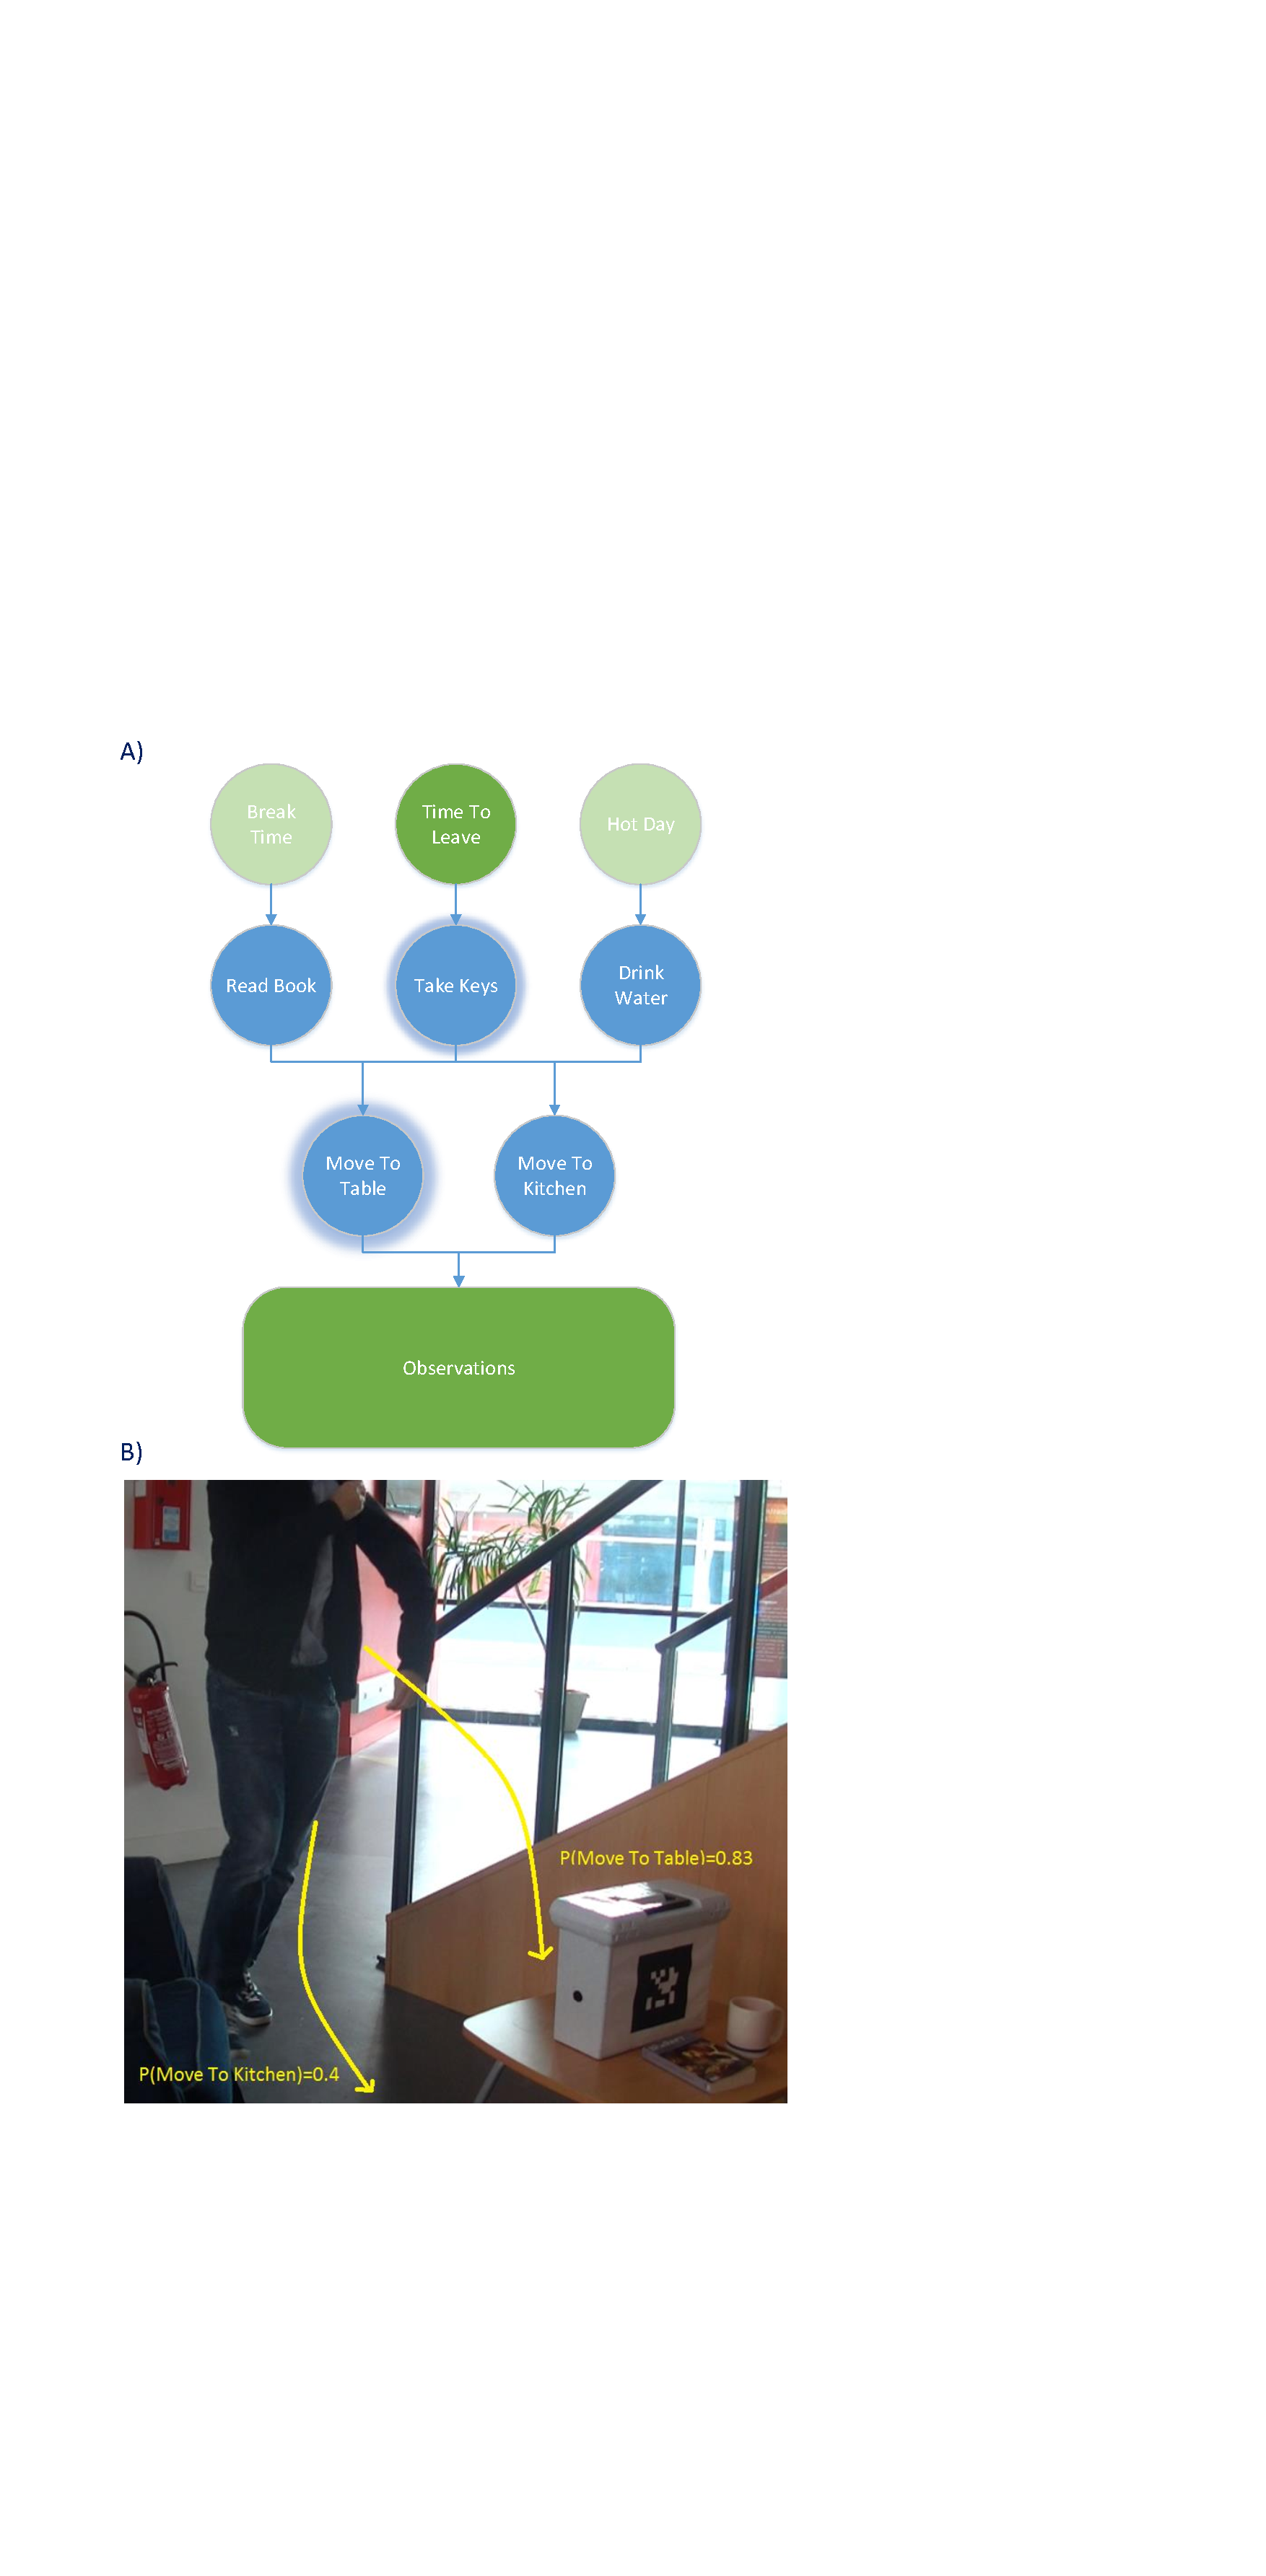
\includegraphics[trim={2cm 11cm 11cm 17cm},clip,scale=0.56]{img/cookieScenario.pdf}
	\caption{Une scène d'expérimentation. Les flèches jaunes montrent les actions possibles et leurs probabilités associées. Le diagramme représente l'IG (Intention Graph) associé. Les cercles verts représentent les nœuds considérés comme preuves et les bleus sont les autres nœuds. Pour les nœuds de contexte, situés en haut du graphe, les nœuds ayant une valeur fausse sont grisés. Parmi les autres nœuds, ceux ayant la probabilité la plus forte sont entourés. Les nœuds d'observation ont étés regroupés en un seul bloc pour simplifier le diagramme.}
	\label{fig:intention_graph}
   	\vspace{-20pt}
\end{figure}

\subsection{Du contexte à l'intention}
Nous introduisons un ensemble de contextes dans notre domaine. Nous considérons comme contexte n'importe quelle information qui peut être utilisée pour caractériser et motiver une intention \cite{abowd1999towards}. Nous modélisons un contexte sous la forme d'une propriété, qui peut prendre différentes valeurs et influencer la probabilité d'un utilisateur d'avoir une intention donnée. Par exemple, on établit qu'un humain a plus de chances de vouloir cuisiner à l'heure du dîner, ou de boire une boisson chaude lorsqu'il fait froid.

Les nœuds de contexte peuvent directement influencer un ou plusieurs nœuds d'intention. Dans notre approche, nous avons choisi d'apprendre ces dépendances conditionnelles directement de l'homme, comme expliqué dans la partie \ref{sec:expeRobotIntent}.

\subsection{De l'intention à l'action}
\label{action_evaluation}
Pour comprendre comment les actions sont liées aux intentions, il faut pouvoir répondre à la question: quelles actions ferait un humain, dans cette situation, étant donné son état de croyance sur l'état du monde, pour accomplir l'objectif lié à son intention? 
Notre démarche est basée sur le principe de rationalité \cite{Dennet1989}, qui affirme que les agents ont tendance à, étant donné leur état de croyance, choisir l'action qui leur semble la plus efficace, afin d'atteindre leur but.

Dans \cite{Blakemore2001}, les auteurs expliquent que "l'attribution des intentions aux actions pourrait reposer sur l'identification de l'action observée et sa correspondance dans notre propre représentation de l'intention". Nous suivons cette idée en donnant au robot un ensemble de modèles de planification. Chacun de ces modèles de planification est relié à une intention, et représente l'ensemble des plans associés permettant d'atteindre le but de l'intention. Grâce à cela, nous pouvons quantifier la correspondance de l'action humaine avec un plan donné, qui est lui même associé à une intention. En d'autres termes, cela permet de répondre à la question "Est-ce que l'humain pense que l'action qu'il vient de faire lui permet d'atteindre tel ou tel but lié à telle ou telle intention".

Dans notre implémentation, pour chaque intention connue par le système, nous créons un Processus de Décision Markovien (MDP pour Markov Decision Process) associé, pour représenter tous les plans possibles liés à cette intention. Un MDP modélise le processus de décision pour un agent dans des situations où le résultat d'une action est partiellement aléatoire, et peut amener à plusieurs résultats. De façon formelle, un MDP est un tuple  \((Q,A,T,R,\gamma)\), où $Q$ est l'état du système, $A$ est un ensemble d'actions, $T(s,a,s')$ est la probabilité que réaliser l'action $a$ dans l'état $s$ mènera à un état $s'$, $R(s,a)$ est la récompense que l'agent obtiendra après avoir réalisé l'action $a$ dans l'état $s$ et \(\gamma\) est un facteur d'actualisation.

% In our implementation, for each intention known by the robot, we will create an associated Markov Decision Process (MDP), to represent all the possible plans associated to this intention. A MDP models the decision process of an agent in situations where the result of an action is partly random, and can lead to several outcomes. Formally a MDP is a tuple \((Q,A,T,R,\gamma)\), where $Q$ is the system state, $A$ is a set of actions, $T(s,a,s')$ is the probability that taking action $a$ in state $s$ will lead to state $s'$, $R(s,a)$ is the reward that the agent will gain after performing action $a$ in state $s$ and \(\gamma\) is a discount factor.

Le souci principal des MDPs est de déterminer la fonction \(\pi(s)\) définissant la politique optimale qui associe la meilleure action à chaque état. "Meilleur" signifie ici que nous cherchons l'action qui maximise le gain de la récompense sur un horizon potentiellement infini. Il y a plusieurs algorithmes bien connus pour calculer la politique d'un MDP (voir \cite{2012Mausam}). En utilisant ces algorithmes nous pouvons également calculer, pendant l'apprentissage, la fonction de valeur d'action \(Q(s,a)\) qui associe à un état $s$ et une action $a$ la récompense attendue sur un horizon actualisé infini. Cette fonction est un point essentiel dans notre approche du problème d'estimation de l'intention.



Nous allons à présent expliquer comment nous utilisons la fonction de valeur d'action pour créer des dépendances conditionnelles entre nœuds d'intention et nœuds d'action dans l'IG. Commençons par définir \(P(a|I_i=1)\), la probabilité que l'action $a$ soit réalisée si l'intention $I_i$ est vraie. Nous modélisons cette probabilité comme \(P(a|I_i=1)=\frac{Q_i(s,a)}{\sum_b(Q_i(s,b))}\), où nous normalisons la fonction de valeur $Q_i(s,a)$ pour l'intention $i$ et l'action $a$ dans l'état de croyance de l'homme $s$, divisé par la fonction de valeur $Q_i(s,b)$ calculée sur toutes les actions surveillées $b$. Nous pouvons étendre ce calcul au cas où un nombre générique d'intentions sont vraies pour calculer la probabilité des nœuds d'action: \(P(a|I_1,I_2,...,I_m)=\frac{\sum_{i:I_i=1}Q_i(s,a)}{\sum_b\sum_{i:I_i=1}Q_i(s,b)}\).

L'idée principale dans ce problème est d'utiliser les croyances de l'humain comme entrées des fonctions de valeurs des MDPs. De cette façon, nous utilisons la prise de perspective au niveau de la planification. Cela traduit le fait que l'humain a des actions cohérentes avec son intention dans son propre état de croyance. Ainsi, même dans la situation où l'homme a des actions qui semblent incohérentes par rapport à l'état du monde courant (par exemple dans le cas où il a une croyance erronée), l'utilisation de la prise de perspective permet malgré tout de les interpréter et de les relier à une intention.

%Our idea is similar to \cite{karami2010human}, where human intentions are estimated using a POMDP and a set of MDPs, that simulate human policies related to different intentions. In this work we use a BN instead of a POMDP, which allows us to separate the mechanisms used for inference and for the robot's actions. Also, we improve the recognition process by including the belief state of the human.

\subsection{De l'action aux observations}
\label{sec:action}
Les intentions sont déduites des actions humaines, donc le robot a besoin de surveiller leur exécution.
Dans notre étude, les actions possibles de l'homme sont des actions de manipulation d'objet. Il nous faut donc pouvoir observer les mouvements de l'homme par rapport aux objets avec lesquels il peut interagir. Pour chaque nœud d'action nous définissons un ensemble de quatre nœuds d'observation: la distance du corps de l'humain à la $cible$ de l'action, la variation de celle-ci, la distance de la main de l'humain à la $cible$ de l'action, et la variation de celle-ci.
Les dépendances conditionnelles des nœuds d'observation sont pré-calculées.

\subsection{Déduction d'intention et d'action}
\label{sec:intentionactioninf}
Nous supposons ici, qu'à chaque moment, un humain ne peut exécuter qu'une action à la fois et que le robot réagira seulement à l'intention la plus probable. L'action et l'intention la plus probable sont déduites du BN de la façon suivante. 

\begin{itemize}
\item $P(n)$ est la probabilité inférée d'un nœud $n$.
\item $B(n)$ est l'ensemble des frères de $n$ (c'est à dire les nœuds de la même couche).
\item $\delta_1$, $\delta_2$ sont deux seuils.
\end{itemize}

Le robot déduit qu'une action a été réalisée, ou qu'un humain a une intention en suivant ces règles:

\begin{enumerate}
\item \(P(n_i)>\delta_1\) 
\item \(\forall b \in B(n_i): P(n_i)>P(b)+\delta_2\)
\end{enumerate}

$n_i$ étant le nœud associé à l'intention ou l'action concernée.
La première condition permet de s'assurer que l'action ou l'intention est suffisamment probante et la seconde permet quant à elle de vérifier qu'elle se démarque des autres actions ou intentions potentielles.

Pour illustrer ces règles, on reprend l'exemple présenté en \ref{fig:intention_graph}.
Deux actions sont alors possible: $MoveToTable$ et $MoveToKitchen$.
Imaginons dans un premier temps qu'on ait:

\begin{itemize}
\item $P(MoveToKitchen) = 0.4$
\item $P(MoveToTable) = 0.83$
\item $\delta_1 = 0.7$
\item $\delta_2 = 0.5$
\end{itemize}

Dans cette situation, la première règle est valide pour l'action $MoveToTable$ (car $P(MoveToTable) > \delta_1$) et est invalide pour $MoveToKitchen$ (car $P(MoveToTable) < \delta_1$). Cela signifie que l'action $MoveToTable$ est suffisamment probable pour être considérée comme acceptable et non $MoveToKitchen$. Cependant, on a  $P(MoveToTable)<P(MoveToKitchen)+\delta_2$ La seconde condition n'est donc pas respectée. Cela signifie que, étant donné les seuils choisis, l'action de se diriger vers la table ne se démarque pas suffisamment, en terme de probabilité, des autres actions possibles (ici en l'occurrence de l'action $MoveToKitchen$).
Ces deux règles permettent de réduire les faux positifs lorsqu'une situation est ambiguë.

Lorsque le robot déduit qu'une action a été réalisée, il met à jour l'état du monde avec ses $postconditions$, déclenchant une mise à jour des croyances de tous les agents présents. Lorsque le robot déduit l'intention actuelle de l'homme, il choisit une réaction possible, comme expliqué dans la section \ref{sec:robot_reaction}.



%%%%%%%%%%%%%%%%%%%%%%%%%%%%%%%%%%%%%%%%%%%%%%%%%%%%%%%%%%%%%%%%%%%%
\section{Comportements pro-actifs}
\label{sec:robot_reaction}

Une fois que le robot est parvenu à estimer l'intention la plus probable, il peut essayer d'aider l'homme à atteindre son but. Nous définissons deux types d'attitudes proactives que le robot peut exécuter à tout moment: corriger l'état de croyance de l'homme et accomplir une partie du plan pour atteindre le but.

\subsubsection{Correction de l'état de croyance}
Avoir une croyance erronée ou incomplète sur l'environnement peut amener l'agent à exécuter des actions non optimales, inutiles, voir contre-productives ou dangereuses. Le robot a besoin de détecter ces situations afin de prévenir l'homme pour que celui-ci puisse corriger son état de croyance et accomplir les actions appropriées. Le robot suppose ici qu'il a toujours un état de croyance correct. Notre solution utilise la récompense attendue de l'action, introduite dans la partie \ref{action_evaluation}. Le principe est de comparer la récompense attendue lors de l'accomplissement d'une action, pour l'humain d'une part (basé sur son modèle de croyance) et pour le robot d'autre part. En d'autres termes, nous regardons si l'homme a une croyance erronée (différente du robot) sur l'influence que son action aura sur l'accomplissement du but. Pour formaliser: nous comparons la valeur d'action \(Q_m(s_h,a_h)\) et \(Q_m(s_r,a_h)\), où $m$ est l'intention la plus probable, $s_h$ et $s_r$ sont les états de croyance de l'homme et du robot, et $a_h$ est l'action la plus probable. Si ces valeurs ne sont pas égales, cela signifie que l'homme attend un résultat de son action qui est différent de ce qu'il va réellement faire.

Nous proposons une solution simple, où le robot prévient l'homme de la croyance divergente détectée pour cette action. Par exemple, Bob veut boire du thé contenu dans une bouteille opaque. Cependant, le robot sait que cette bouteille est vide (par exemple parce qu'un agent a bu le dernier verre), mais Bob l'ignore. Lorsqu'il s'approche de la bouteille, le robot détecte que l'intention la plus probable (en utilisant le processus décrit en \ref{sec:intention_recognition}) est de boire du thé. Le système calcule la récompense attendue par l'action de prendre la bouteille dans le modèle de Bob et du robot afin de modéliser l'avancement du plan attendu par cette action par rapport à l'état de croyance de chacun. On obtient des valeurs différentes. Ici la valeur est plus élevée pour Bob signifiant qu'il pense que son action aura une conséquence "meilleure" (qui fera avancer l'état du monde vers son but) que celle prévue par le robot (la récompense dans l'état mental du robot étant inférieure). Le système vérifie les valeurs des propriétés associées à la bouteille dans les deux modèles mentaux et en extrait celles qui sont divergentes. En utilisant cette information, le robot corrige la croyance divergente en informant l'humain que la bouteille ne contient plus de thé.

% In critical tasks, it may be important that the human has always a complete and correct belief state. In this situation, when the robot detects a human intention, it can check if there is a divergence between its and the human's belief states, and inform the human of this difference in order to synchronize their belief states, before even monitoring its actions.
% Same for the following paragraph, using " the robot" make it sounds like it's magic XD

\subsubsection{Réalisation d'une partie du plan}
\label{robot_acts}
Il y a des situations dans lesquelles le robot devrait aider l'homme à accomplir son but en agissant. Dans ces cas là, le robot crée un plan partagé pour accomplir le but lié à l'intention reconnue, et exécute les actions qui lui incombent. Le robot est capable de surveiller les actions de l'homme et replanifier si ses actions diffèrent du plan qu'il a établi, permettant ainsi d'être flexible aux choix de l'homme et de s'adapter dynamiquement de la même façon que décrite en \cite{fioreiser2014}.
\vspace{-5pt}


\section{Étude expérimentale}
\label{sec:experimentsIntent}
%TODO ajouter plein d'illustrations!
Pour estimer les performances de notre système en terme de reconnaissance d'intention, nous voulons mener une étude expérimentale. Le problème est que les intentions humaines ne sont pas directement observables. Une des façons de procéder est présentée dans \cite{baker2014modeling}. Nous allons comparer l'estimation de l'intention humaine faite par d'autres humains avec la prédiction de notre système. Afin de pouvoir réaliser cette comparaison nous avons effectué une étude utilisateur où nous avons montré aux participants plusieurs vidéos, leur demandant d'estimer la probabilité d'un ensemble d'intentions pour chaque vidéo, puis nous avons regroupé ces résultats.

Nous avons réalisé un test d'équivalence TOST (Two One-Sided Test) où nous comparons les intentions telles qu'elles ont été estimées par les humains avec les estimations du robot. Nous choisissons comme seuil pour l'équivalence la déviation standard $\sigma$ des réponses des utilisateurs. L'idée derrière ce choix est que, si la réponse du robot est plus proche que la déviation standard de la réponse moyenne des humains, ses prédictions sont comparables à la réponse d'un utilisateur moyen présent dans notre groupe d'utilisateurs. 

Nous définissons nos hypothèses:

\begin{enumerate}
\item $H_0$: $\mu_{hi}-\mu_{ri}\leq-\sigma_{hi}$ OU $\mu_{hi}-\mu_{ri}\geq\sigma_{hi}$
\item $H_A$: $-\sigma_{hi}<\mu_{hi}-\mu_{ri}<\sigma_{hi}$
\end{enumerate}

Où $\mu_{hi}$ et $\mu_{ri}$ sont la moyenne humaine et la réponse du robot pour le test $i$, $\sigma_{hi}$ est la variance des réponses humaines pour le test $i$.

Nous avons effectué des tests pour évaluer: a) la prédiction sans indices (No clues), b) la prédiction en présence d'indices contextuels (Contextual clues), c) la prédiction en présence d'indices sur l'état mental (Divergent belief).

Nous établissons un environnement avec un ensemble de meubles: une \textit{Étagère de Cuisine}, une \textit{Table}, un \textit{Canapé}, et une \textit{Chaise}. Dans cet environnement, nous avons créé deux scénarios, dans lesquels se déroulent plusieurs tests, avec deux humains, \textit{Max} et \textit{Bob}, qui réalisent différentes actions. chaque scénario contient une collection d'objets, et un ensemble d'intentions préétablies. Pour les tests relatifs aux états de croyances, nous commençons par montrer aux utilisateurs et au robot une séquence d'événements, leur permettant de construire un modèle d'état mental pour les agents. Nous allons détailler les deux scénarios et les tests s'y rapportant.

\subsubsection{Scénario des cookies}
\begin{itemize}
\item Objets: une \textit{Boîte de cookie}, un \textit{Mug}, et une \textit{Bouteille d'eau} sont placés sur une \textit{Table}, proches les uns des autres comme exposé dans l'image \ref{fig:cookieScen}. Un paquet de \textit{Cookies} est placé dans l'\textit{Étagère de cuisine}. La \textit{Boîte de cookie} peut contenir ou non des \textit{Cookies}.
\item Intentions: manger un cookie (\textit{Eating a cookie}), boire de l'eau (\textit{Drinking water}), et lire un livre (\textit{Reading the book}).
\item Tests:
\begin{itemize}
	\item \textit{No clues}: \textit{Max} s'approche de la \textit{Table}.
    \item \textit{Contextual clues}: \textit{Max} s'approche de la \textit{Table} en faisant un commentaire sur la chaleur ambiante.
	\item \textit{Divergent belief Max}: \textit{Max} s'approche de la \textit{Table}.
	\item \textit{Divergent belief Bob}: \textit{Bob} s'approche de la \textit{Table}.
\end{itemize}
\item  \textit{Événement de croyance divergente}:  \textit{Max} et \textit{Bob} discutent sur le \textit{Canapé}. Max mange le dernier \textit{Cookie} de la \textit{Boîte de Cookie} avant de la refermer et de sortir. Pendant que \textit{Max} est parti, \textit{Bob} prend des \textit{Cookies} de l'\textit{Étagère de la cuisine}, remplit la \textit{Boîte de cookies}, et la referme, avant de partir.
\end{itemize}

\begin{figure}[ht!]
  \centering
 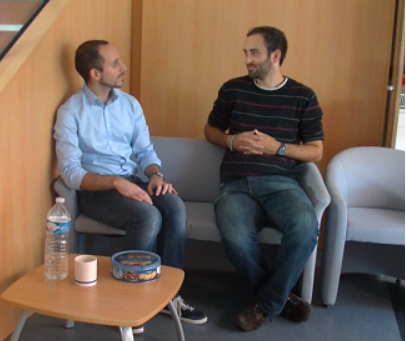
\includegraphics[width=0.7\linewidth]{./intention/actors.png} 
  \caption {Image représentant la configuration du scénario des cookies issu des vidéos présentées aux humains chargés d'estimer les intentions.}
  \label{fig:cookieScen}
\end{figure}

L'\textit{Événement de croyance divergente} a été montré aux utilisateurs et au robot entre le test \textit{Contextual clues} et le test \textit{Divergent belief Max}. 

Nous avons volontairement inclus une intention, \textit{Reading the book}, sans mettre de livre dans l'environnement visible, afin d'introduire un élément incertain dans le scénario.

\subsubsection{Scénario des clés}
\begin{itemize}

\item Objets: Une \textit{Boîte} est placée sur une \textit{Table}. La \textit{Boîte} cache partiellement la vue des personnes qui approchent. Un \textit{Livre} et un \textit{Mug} sont placés derrière la \textit{Boîte}, afin qu'ils puissent être vus depuis le \textit{Canapé} mais pas des gens qui s'approchent. Pour illustrer la configuration, une image extraite de la vidéo est présentée à la figure \ref{fig:keyScen}.

\item Intentions: prendre le \textit{Mug} \textit{Taking the mug}, prendre les \textit{clés} \textit{Taking the keys}, lire un \textit{Livre} \textit{Reading the book}.



\begin{figure}[ht!]
  \centering
 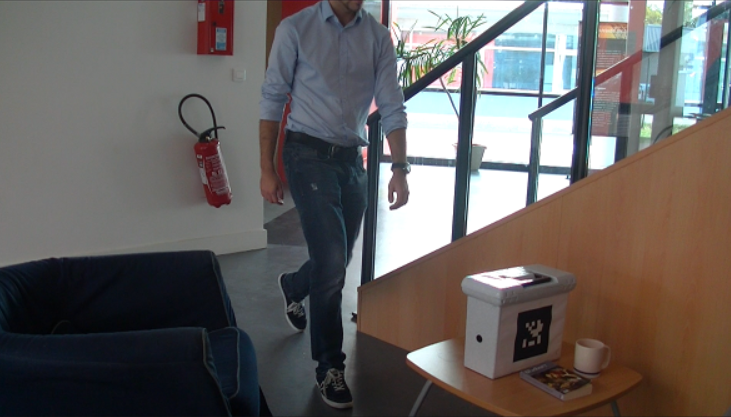
\includegraphics[width=0.8\linewidth]{./intention/keys1.png} 
  \caption {Image représentant la configuration du scénario des clés issue des vidéos présentées aux utilisateurs chargés d'estimer les intentions.}
  \label{fig:keyScen}
\end{figure}


\item Tests et événements:
\begin{itemize}
\item \textit{No clues}: \textit{Max} s'approche de la \textit{Table}.
\item\textit{Contextual clues}: \textit{Max} s'approche de la \textit{Table} en hâte, tout en enfilant un manteau.
\item \textit{Divergent belief Max}: \textit{Max} s'approche de la \textit{Table} en hâte, tout en enfilant un manteau.
\end{itemize}

\item \textit{Événements de croyance divergente}: \textit{Max} est assis sur le \textit{Canapé}, buvant dans le \textit{Mug}, et ayant les \textit{Clés} en mains. Son téléphone sonne, il pose les \textit{Clés} et le \textit{Mug} sur la \textit{Table}, derrière la \textit{Boîte}, et quitte la salle. Pendant que \textit{Max} est absent, \textit{Bob} arrive et prend place sur le \textit{Canapé}, lisant un \textit{Livre}. Lorsqu'il voit les \textit{Clés}, il pose le \textit{Livre} sur la \textit{Table} et prend les \textit{Clés} pour les amener aux objets trouvés.
\end{itemize}

L'\textit{Événement de croyance divergente} est montré aux utilisateurs et au robot entre les événements de \textit{Contextual clues} et \textit{Divegent belief Max}.

\subsection{Étude utilisateurs}
Pour collecter les estimations d'intentions de la part d'humains, nous avons créé une étude en ligne, où nous présentons des vidéos en relation avec les tests et événements des deux scénarios. Les utilisateurs ont estimé la probabilité de chaque intention disponible sur une échelle de Likert à 5 niveaux. L'étude a été réalisée en trois langues, avec des utilisateurs résidents dans différents pays \footnote{Une version de cette étude est fournit à l'adresse http://goo.gl/forms/gWwdIutbOCUk3vdx2}. Nous avons recueilli les réponses de 78 adultes, calculé la moyenne de chaque réponse puis nous avons converti ces moyennes en pourcentages, afin de les comparer aux réponses du robot.

Lorsqu'on observe les réponses des utilisateurs (voir figure \ref{fig:user_study_results}), nous observons que, dans l'absence d'indices, les individus ont donné la même note aux différentes intentions liées aux objets visibles. Les indices de contexte ont eu la plus grosse influence sur les réponses des utilisateurs. Cela est particulièrement visible dans le test \textit{Contextual Clues} du scénario des clés (\textit{Keys Scenario}), où les utilisateurs ont noté comme intention la plus probable \textit{Take Keys}, même si aucune clé n'était visible dans la vidéo. Les croyances divergentes ont également influencé l'estimation des humains, mais dans une proportion moins importante. Globalement, les réponses les plus fortes, ont été données par le test \textit{Divergent Belief Max} sur le scénario des clés, qui utilise à la fois des indices de contexte et la connaissance de l'état mental divergent.

\subsection{Implémentation robotique}
\label{sec:expeRobotIntent}
Nous avons répliqué les deux scénarios avec un robot PR2 de Willow Garage\footnote{https://www.willowgarage.com/pages/pr2/overview}. Nous avons simplifié la perception, en utilisant de la capture de mouvement pour suivre les humains. Pour la détection d'objet nous utilisons un logiciel de reconnaissance de tags \footnote{Des vidéos d'expériences associées peuvent être vue sur  http://homepages.laas.fr/mfiore/roman2016.html}. 

Au début d'un scénario, le robot scanne l'environnement, construisant un modèle de l'état du monde. Avec notre perception, il n'est pas possible de savoir si la boîte de cookie est pleine ou vide et nous la considérons donc comme pleine au commencement d'un test, et ses valeurs sont mises à jour en utilisant les $postconditions$ (effets) des actions humaines inférées. Nous considérons que la boîte est vide lorsqu'un humain prend un cookie, et comme pleine lorsqu'un humain y met un cookie.

Nous avons construit différents IGs pour les scénarios. Chaque test a un graphe différent, lié à l'agent principal dont on veut reconnaître l'intention. Nous considérons trois différents nœuds de contexte pour ces IGs: \textit{HotDay}, qui est vrai lorsque la journée est particulièrement chaude; BreakTime, qui est vrai lorsque les agents prennent une pause; TimeToLeave, qui est vrai lorsqu'il est tard dans la journée, et que les humains partent en général de leur lieu de travail pour rentrer chez eux.

Comme indiqué précédemment, nous avons choisi de suivre \cite{Liu2014} afin d'apprendre le lien entre contexte et intention. Nous avons fait une petite étude utilisateur avec 15 personnes, dans laquelle 5 scénarios ont été présentés. Chaque scénario est lié à une des intentions utilisées dans nos tests. Pour chaque scénario, nous avons demandé aux utilisateurs de noter le lien perçu entre l'intention et les trois contextes. Pour ce faire, les individus ont noté la "force" de ce lien sur une échelle de Likert à cinq niveaux. Nous avons utilisé la moyenne des réponses pour calculer la probabilité de la dépendance conditionnelle entre les nœuds de contexte et les nœuds d'intention.


Dans le scénario  du cookie (\textit{Cookie Scenario}) le graphe pour les tests est construit à partir des nœuds suivants:
\begin{itemize}
\item Nœuds de contexte: \textit{Hot Day}, \textit{Break Time}, \textit{Time to Leave}
\item Nœuds d'intention: \textit{Fill Cookie Box}, \textit{Eat Cookie}, \textit{Drink Water}, \textit{Read Book}.
\item Nœuds d'action: \textit{Move to Table}, \textit{Move to Kitchen}.
\item Nœuds d'observation: distance du corps de l'agent et de sa main à chaque cible d'action.
\end{itemize}

Nous introduisons l'intention de remplir la boîte de cookie (\textit{Fill Cookie Box}), qui n'est pas présente dans les tests soumis aux humains, afin que le robot détecte lorsque Bob remplit la boîte de cookies pendant l'événement de croyance divergente.

Notre robot, dans cette expérimentation, n'est pas équipé de capacité pour comprendre la parole de l'homme, et assigne directement les nœuds de contexte à des valeurs plausibles et qui pourraient être acquises en regardant les vidéos. Pour le test de \textit{Contextual Clues}, nous assignons la valeur de \textit{Hot Day} à vrai (dans la vidéo Max commente la chaleur du jour), et \textit{Break Time}, et \textit{Time to Leave} à faux (car aucun élément dans la vidéo n'indique que ces contextes sont vrais).

%. Max and Bob seem to have taken a break from work before the other events are shown, in the Divergent Belief Event).

L'événement de croyance divergente (\textit{Divergent Belief Event}), le test \textit{Divergent Belief Max}, et le test \textit{Divergent Belief Bob} ont été montrés dans cet ordre au robot, qui a pu ainsi suivre et mettre à jour les états de croyance des agents et créer les nouveaux IGs qui conviennent à cette situation. Pendant l'événement de croyance divergente, plusieurs IGs ont étés créés avec différents nœuds d'action et d'observation, pour suivre la séquence d'action réalisée par les deux agents. Par exemple, quand \textit{Max} quitte la pièce, \textit{Bob} a la possibilité d'exécuter les actions \textit{Take Mug}, \textit{Take Water Bottle}, \textit{Open Cookie Box}, \textit{Move to Kitchen Shelf} ou \textit{Leave Room}. Les nœuds d'intention et de contexte restent quand à eux inchangés dans tous les IGs du scénario.


Le scénario des clés (\textit{Keys Scenario}) a un IG, avec les différences suivantes:
\begin{itemize}
\item Nœuds de contexte: \textit{Hot Day}, \textit{Break Time} et \textit{Time to Leave}.
\item Nœuds d'intention: \textit{Drink Water}, \textit{Take Keys}, \textit{Read Book}.
\end{itemize}

Les nœuds d'action et d'observation sont les mêmes que le scénario précédent et suivent les mêmes idées durant l'événement de croyance divergente. Un exemple d'IG utilisé dans les tests est présenté à la figure \ref{fig:intention_graph}. Pour les tests \textit{Contextual Clues} et \textit{Divergent Belief}, nous mettons la valeur contextuelle \textit{Time to Leave} à vrai (Max met un manteau et semble pressé), et les autres valeurs contextuelles à faux. En utilisant le composant décrit dans les sections précédentes, et ces IGs, le robot a été capable d'obtenir des prédictions à partir des actions des utilisateurs.

\subsection{Discussion}
\label{discussion}
Nous réalisons des tests TOST pour chaque intention contenu dans les scénarios, en comparant les réponses des humains avec celles du robot pour un total de 21 tests.

Nous calculons les p-valeurs et réalisons nos tests en utilisant la valeur de signification $\alpha=0.05$.

En analysant les résultats de nos tests d'équivalence, présentés dans la figure \ref{fig:user_study_results}, des informations intéressantes peuvent en être extraites. 1) Le comportement de notre système est généralement proche des capacités humaines. 19 tests sur les 21 valident notre hypothèse avec une p-valeur inférieure à la valeur de signification. 2) Le contexte et l'état de croyance de l'homme sont à prendre en compte. Un système qui ignorerait ces deux facteurs aurait pu reconnaître correctement que l'intention du test \textit{No Clues}. 3) Certains raisonnements présents chez l'homme sont encore manquants dans notre système. Nous avons échoué à rejeter l'hypothèse nulle pour deux cas. Dans \textit{Divergent Belief Bob} les humains ont donné une note plus importante à l'intention \textit{Eat Cookie} que l'intention \textit{Drink Water}. Une explication est qu'ils ont pensé que, étant donné que \textit{Bob} a rempli la \textit{Boîte de cookies}, il y a plus de chance qu'il souhaite manger un \textit{Cookie}. Cela permet de penser que l'homme utilise des raisonnements temporels complexes pour évaluer l'intention, en considérant tout l'historique des actions des agents pour deviner leur intention.



 \begin{figure}[h!]
	\centering
	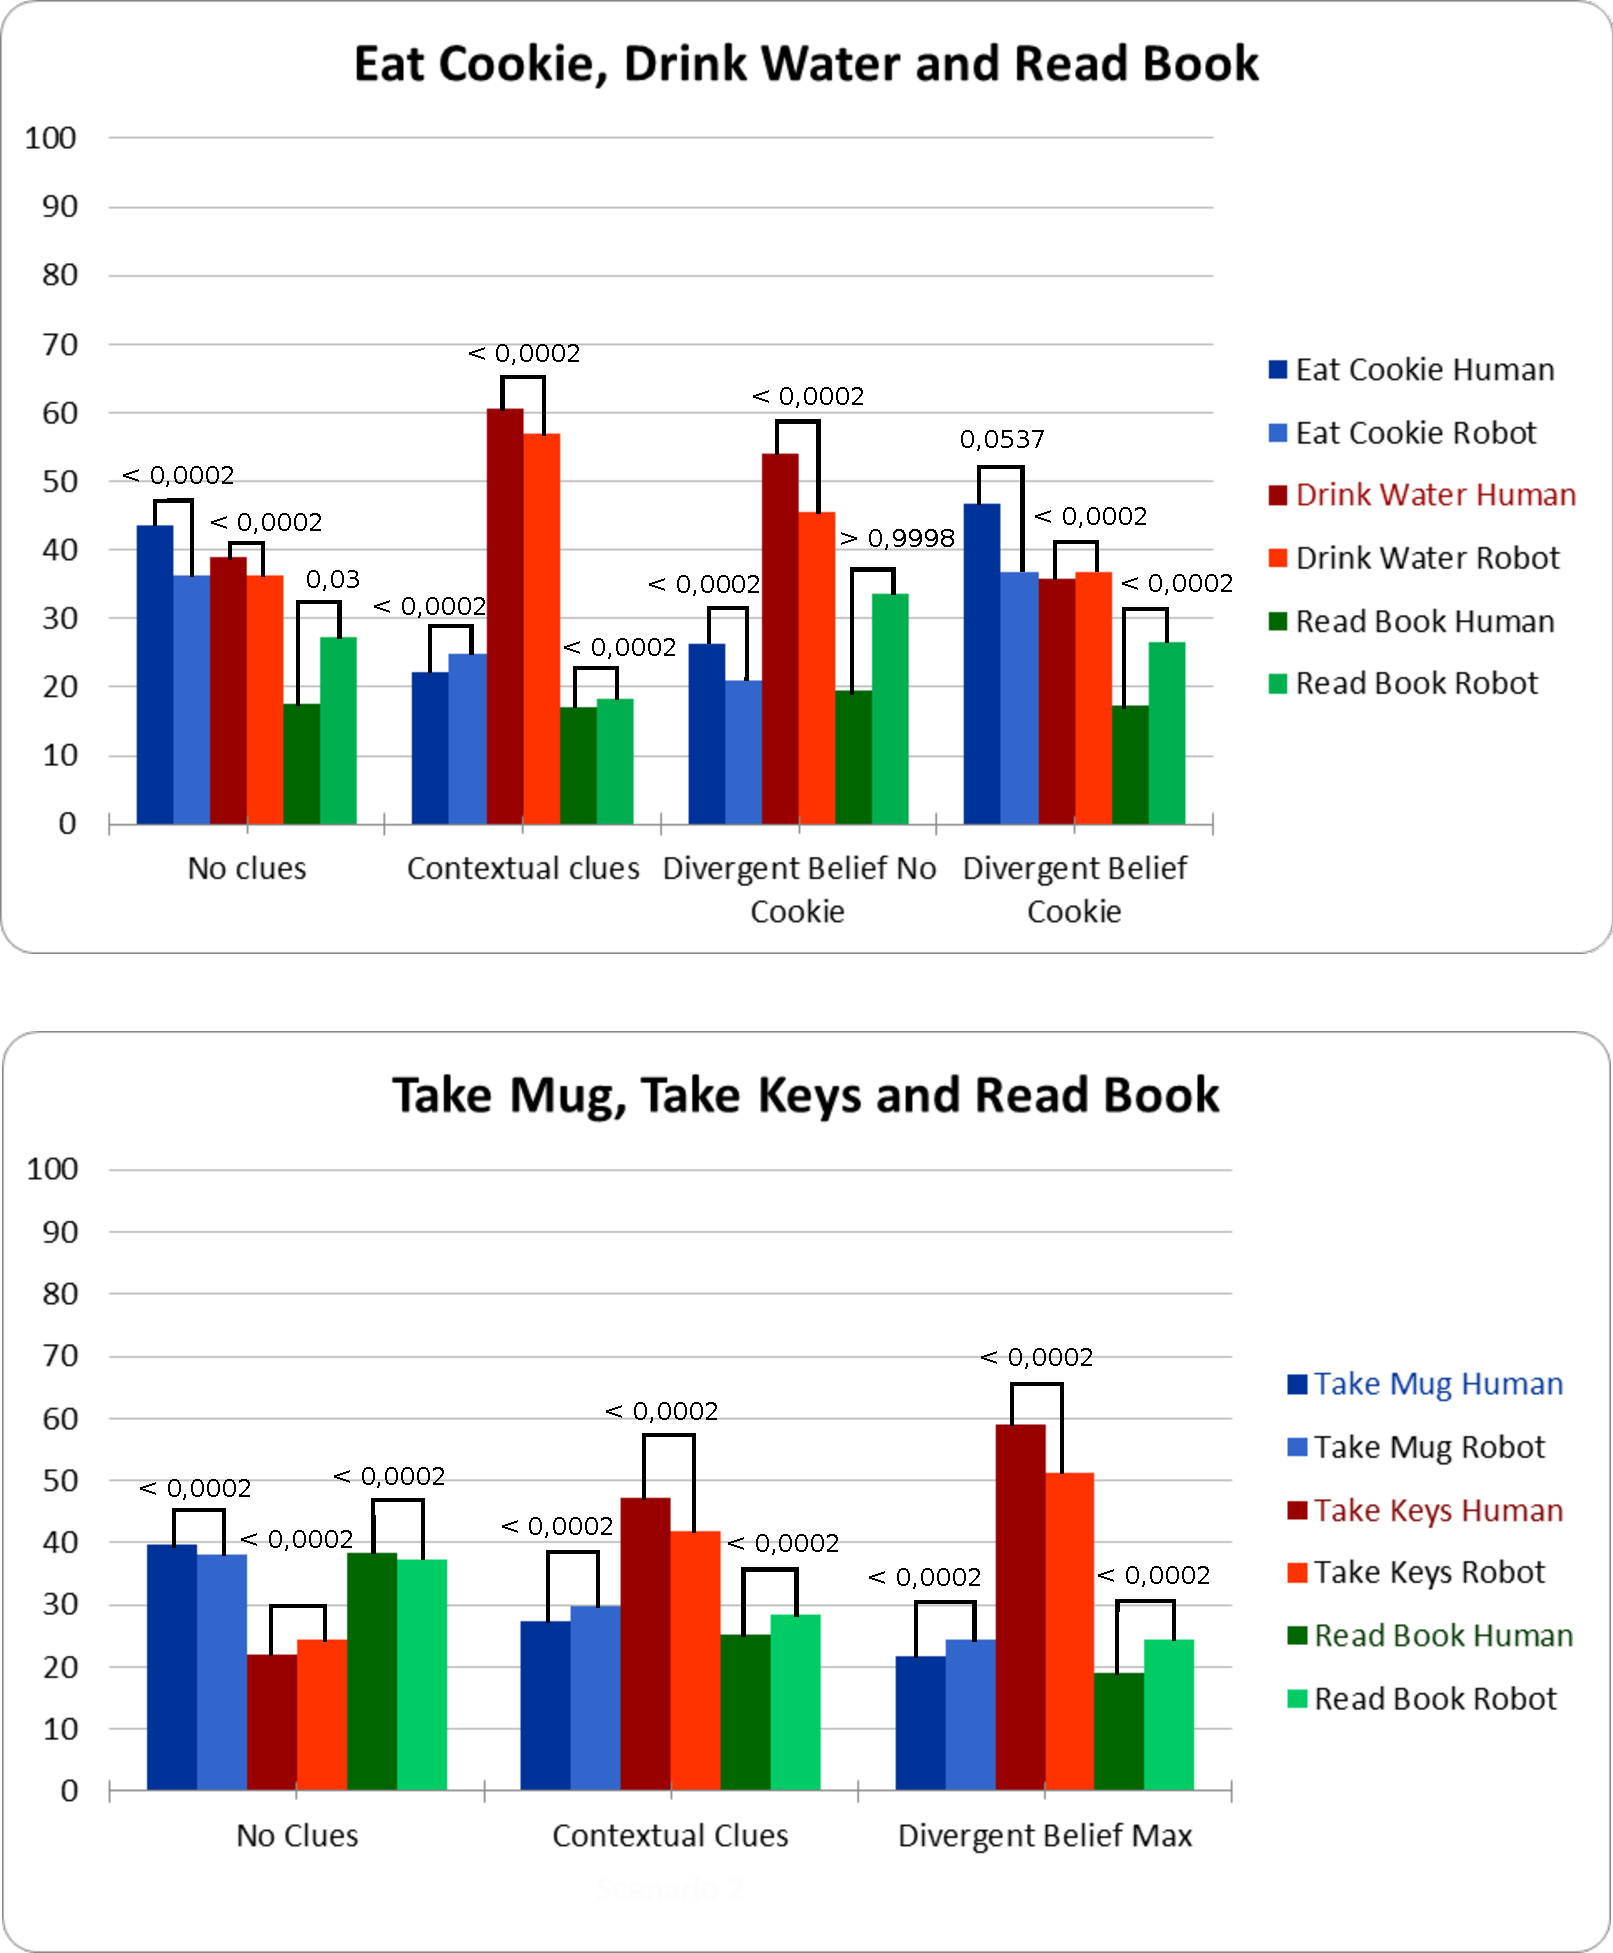
\includegraphics[clip,scale=0.52]{img/pvalues1.pdf}
	\caption{Résultats expérimentaux. Les résultats pour les deux scénarios sont représentés sous forme de graphes. Les intentions, estimées par les hommes et le système de reconnaissance d'intention, sont représentées sous différentes couleurs (voir légende). L'estimation des mêmes intentions par le système et par les hommes sont placées côte à côte. Chaque colonne représente la probabilité d'une intention exprimée en pour-cent. Les P-valeurs du test d'équivalence sont ajoutées au graphe.}
	\label{fig:user_study_results}
  	\vspace{-16pt}
\end{figure}


\section{Conclusion}
Dans ce chapitre, nous avons présenté un système capable d'évaluer les intentions humaines en utilisant la gestion de la croyance, les données contextuelles et l'observation d'actions. Nous avons effectué une étude sur les utilisateurs où nous avons comparé les prédictions de notre système avec ceux des humains. Dans cette étude, nous avons montré que notre système est en mesure, dans plusieurs situations, d'approcher les capacités humaines. Notre système utilise la prédiction de l'intention afin d'aider de manière proactive les humains à atteindre leurs objectifs en effectuant une partie du plan ou en corrigeant verbalement leur état de croyance.

Les résultats obtenus mettent également en valeur que les humains utilisent probablement des raisonnements temporels pour désambiguïser les intentions (comme indiqué dans la section \ref{discussion}). Il serait intéressant d'étudier d'avantage ces mécanismes et d'utiliser notre base de données temporelles présentée en \ref{sec:dbt} pour ajouter ce type de mécanisme au robot.

Nous supposons, dans ce travail, que le robot a toujours un état de croyance correcte et l'utilise comme une référence pour l'état de l'environnement. Il serait intéressant d'aborder le problème où le robot a un état de croyance erronée, par exemple en analysant le degré de confiance que l'homme semble avoir dans ses comportements.


% In this paper we presented a system able to assess human intentions using belief management, contextual data and action observation. We performed a user study where we compared the predictions of our system with those of humans. In this study, we showed that our system is able, in several situations, to approach human capacities. Our system uses intention prediction to proactively help humans achieve their goals by performing a part of the plan or verbally correcting their belief state.

% The system is flexible and easily extendable by adding new MDP models and planning domains intentions. Most of the computation regarding MDPs is done offline, by calculating the action value functions and storing them in tables, with online computation mainly used for situation assessment, which uses efficient algorithms. Thanks to these aspects our system would be able to include more intentions and to maintain real-time performances.

% There are several possible developments to our system. We could explore the use of more complex models, for example by considering mental beliefs as probabilistic, while trying to maintain an efficient computation time. Learning algorithm could also contribute to our system, by allowing the robot to adapt its recognition process to the behaviors of different users. The result also puts into light that humans might use deeper temporal reasoning to disambiguate intentions (as discussed in section \ref{discussion}), which should be further studied.

% We assume, in this work, that the robot has always a correct belief state and uses it as a reference for the state of the environment. It would be interesting to address the problem where the robot has a wrong belief state, for example by analyzing the degree of confidence that the human seems to have in his behaviors.

\ifdefined\included
\else
\bibliographystyle{acm}
\bibliography{These}
\end{document}
\fi

\ifdefined\included
\else
\documentclass[a4paper,11pt,twoside]{StyleThese}
\usepackage{amsmath,amssymb}             % AMS Math
\usepackage[french]{babel}
\usepackage[utf8]{inputenc}
\usepackage[T1]{fontenc}
\usepackage{tabularx}
%\usepackage{tabular}
\usepackage{multirow}


\usepackage[tight,footnotesize]{subfigure}
\usepackage{algorithm} %To allow algorithm environment
\usepackage{algpseudocode} %Provides algorithmic environment

\usepackage{hhline}
\usepackage[left=1.5in,right=1.3in,top=1.1in,bottom=1.1in,includefoot,includehead,headheight=13.6pt]{geometry}
\renewcommand{\baselinestretch}{1.05}

% Table of contents for each chapter

\usepackage[nottoc, notlof, notlot]{tocbibind}
\usepackage[french]{minitoc}
\setcounter{minitocdepth}{2}
\mtcindent=15pt
% Use \minitoc where to put a table of contents

\usepackage{aecompl}

% Glossary / list of abbreviations

\usepackage[intoc]{nomencl}
\renewcommand{\nomname}{Liste des Abréviations}

\makenomenclature

% My pdf code

\usepackage{ifpdf}

\ifpdf
  \usepackage[pdftex]{graphicx}
  \DeclareGraphicsExtensions{.jpg}
  \usepackage[a4paper,pagebackref,hyperindex=true]{hyperref}
  \usepackage{tikz}
  \usetikzlibrary{arrows,shapes,calc}
\else
  \usepackage{graphicx}
  \DeclareGraphicsExtensions{.ps,.eps}
  \usepackage[a4paper,dvipdfm,pagebackref,hyperindex=true]{hyperref}
\fi

\graphicspath{{.}{images/}}

%nicer backref links
\renewcommand*{\backref}[1]{}
\renewcommand*{\backrefalt}[4]{%
\ifcase #1 %
(Non cité.)%
\or
(Cité en page~#2.)%
\else
(Cité en pages~#2.)%
\fi}
\renewcommand*{\backrefsep}{, }
\renewcommand*{\backreftwosep}{ et~}
\renewcommand*{\backreflastsep}{ et~}

% Links in pdf
\usepackage{color}
\definecolor{linkcol}{rgb}{0,0,0.4} 
\definecolor{citecol}{rgb}{0.5,0,0} 
\definecolor{linkcol}{rgb}{0,0,0} 
\definecolor{citecol}{rgb}{0,0,0}
% Change this to change the informations included in the pdf file

\hypersetup
{
bookmarksopen=true,
pdftitle="Évaluation de la sécurité des équipements grand public connectés à Internet",
pdfauthor="Yann BACHY", %auteur du document
pdfsubject="Thèse", %sujet du document
%pdftoolbar=false, %barre d'outils non visible
pdfmenubar=true, %barre de menu visible
pdfhighlight=/O, %effet d'un clic sur un lien hypertexte
colorlinks=true, %couleurs sur les liens hypertextes
pdfpagemode=None, %aucun mode de page
pdfpagelayout=SinglePage, %ouverture en simple page
pdffitwindow=true, %pages ouvertes entierement dans toute la fenetre
linkcolor=linkcol, %couleur des liens hypertextes internes
citecolor=citecol, %couleur des liens pour les citations
urlcolor=linkcol %couleur des liens pour les url
}

% definitions.
% -------------------

\setcounter{secnumdepth}{3}
\setcounter{tocdepth}{2}

% Some useful commands and shortcut for maths:  partial derivative and stuff

\newcommand{\pd}[2]{\frac{\partial #1}{\partial #2}}
\def\abs{\operatorname{abs}}
\def\argmax{\operatornamewithlimits{arg\,max}}
\def\argmin{\operatornamewithlimits{arg\,min}}
\def\diag{\operatorname{Diag}}
\newcommand{\eqRef}[1]{(\ref{#1})}

\usepackage{rotating}                    % Sideways of figures & tables
%\usepackage{bibunits}
%\usepackage[sectionbib]{chapterbib}          % Cross-reference package (Natural BiB)
%\usepackage{natbib}                  % Put References at the end of each chapter
                                         % Do not put 'sectionbib' option here.
                                         % Sectionbib option in 'natbib' will do.
\usepackage{fancyhdr}                    % Fancy Header and Footer

% \usepackage{txfonts}                     % Public Times New Roman text & math font
  
%%% Fancy Header %%%%%%%%%%%%%%%%%%%%%%%%%%%%%%%%%%%%%%%%%%%%%%%%%%%%%%%%%%%%%%%%%%
% Fancy Header Style Options

\pagestyle{fancy}                       % Sets fancy header and footer
\fancyfoot{}                            % Delete current footer settings

%\renewcommand{\chaptermark}[1]{         % Lower Case Chapter marker style
%  \markboth{\chaptername\ \thechapter.\ #1}}{}} %

%\renewcommand{\sectionmark}[1]{         % Lower case Section marker style
%  \markright{\thesection.\ #1}}         %

\fancyhead[LE,RO]{\bfseries\thepage}    % Page number (boldface) in left on even
% pages and right on odd pages
\fancyhead[RE]{\bfseries\nouppercase{\leftmark}}      % Chapter in the right on even pages
\fancyhead[LO]{\bfseries\nouppercase{\rightmark}}     % Section in the left on odd pages

\let\headruleORIG\headrule
\renewcommand{\headrule}{\color{black} \headruleORIG}
\renewcommand{\headrulewidth}{1.0pt}
\usepackage{colortbl}
\arrayrulecolor{black}

\fancypagestyle{plain}{
  \fancyhead{}
  \fancyfoot{}
  \renewcommand{\headrulewidth}{0pt}
}

%\usepackage{MyAlgorithm}
%\usepackage[noend]{MyAlgorithmic}
\usepackage[ED=MITT - STICIA, Ets=INP]{tlsflyleaf}
%%% Clear Header %%%%%%%%%%%%%%%%%%%%%%%%%%%%%%%%%%%%%%%%%%%%%%%%%%%%%%%%%%%%%%%%%%
% Clear Header Style on the Last Empty Odd pages
\makeatletter

\def\cleardoublepage{\clearpage\if@twoside \ifodd\c@page\else%
  \hbox{}%
  \thispagestyle{empty}%              % Empty header styles
  \newpage%
  \if@twocolumn\hbox{}\newpage\fi\fi\fi}

\makeatother
 
%%%%%%%%%%%%%%%%%%%%%%%%%%%%%%%%%%%%%%%%%%%%%%%%%%%%%%%%%%%%%%%%%%%%%%%%%%%%%%% 
% Prints your review date and 'Draft Version' (From Josullvn, CS, CMU)
\newcommand{\reviewtimetoday}[2]{\special{!userdict begin
    /bop-hook{gsave 20 710 translate 45 rotate 0.8 setgray
      /Times-Roman findfont 12 scalefont setfont 0 0   moveto (#1) show
      0 -12 moveto (#2) show grestore}def end}}
% You can turn on or off this option.
% \reviewtimetoday{\today}{Draft Version}
%%%%%%%%%%%%%%%%%%%%%%%%%%%%%%%%%%%%%%%%%%%%%%%%%%%%%%%%%%%%%%%%%%%%%%%%%%%%%%% 

\newenvironment{maxime}[1]
{
\vspace*{0cm}
\hfill
\begin{minipage}{0.5\textwidth}%
%\rule[0.5ex]{\textwidth}{0.1mm}\\%
\hrulefill $\:$ {\bf #1}\\
%\vspace*{-0.25cm}
\it 
}%
{%

\hrulefill
\vspace*{0.5cm}%
\end{minipage}
}

\let\minitocORIG\minitoc
\renewcommand{\minitoc}{\minitocORIG \vspace{1.5em}}

\usepackage{multirow}
%\usepackage{slashbox}

\newenvironment{bulletList}%
{ \begin{list}%
	{$\bullet$}%
	{\setlength{\labelwidth}{25pt}%
	 \setlength{\leftmargin}{30pt}%
	 \setlength{\itemsep}{\parsep}}}%
{ \end{list} }

\newtheorem{definition}{Définition}
\renewcommand{\epsilon}{\varepsilon}

% centered page environment

\newenvironment{vcenterpage}
{\newpage\vspace*{\fill}\thispagestyle{empty}\renewcommand{\headrulewidth}{0pt}}
{\vspace*{\fill}}

\usepackage{tablefootnote}
\sloppy


\begin{document}
\setcounter{chapter}{4} %% Numéro du chapitre précédent ;)
\dominitoc
\faketableofcontents
\fi

\chapter{Estimation de l'Expertise Humaine et Adaptation de la Collaboration}
\label{chapter5}
\minitoc

\section{Contexte et Motivation}
% Expose the issue of plan verbalizing + why HTN as colaborative plan + why reasoning on agent knowledge
L'un des défis de la robotique est de faire collaborer convenablement les robots avec des partenaires humains durant l'accomplissement de tâches. Collaborer avec un humain nécéssite de la part du robot de plannifier ses propres actions, d'anticiper les contributions de son partenaire au plan global, de surveiller les actions potentiellement complexes de l'homme et de maintenir un état du monde à jour. La collaboration doit, en plus de cela, avoir une dimension sociale suffisamment importante pour garantir le confort de l'homme ainsi qu'une lisibilité des actions et décisions du robot afin que le système soit intuitif. En dernier lieu, le comportement social a également une influence important sur l'accpetation du robot par l'homme.

%Plan generation
Nous définissons un plan collaboratif, ou plan partagé, comme un ensemble d'actions liées, impliquant plusieurs agents qui coopèrent afin d'avancer vers un objectif commun.
Pour générer un plan partagé, le robot devrait prendre en compte non seulement la configuration de son environnement, mais également son/ses partenaire(s) humain(s). Un moyen pragmatique de prendre en compte l'humain consiste à calculer les affordances de celui-ci, lui permettant de générer des plans plus pertinents et pour lesquels l'homme est dans la capacité d'accomplir les tâches qui lui sont confiées. D'un point de vue social, le robot devrait également pouvoir adapter le plan aux préférences et à l'expertise de l'utilisateur. Idéalement, cette adaptation devrait pouvoir se faire au niveau de chaque tâche du plan.

%Plan explanation
Une fois que le robot a généré un plan pour atteindre l'objectif des agents impliqués, il faut pouvoir le partagé avec le partenaire humain afin de s'assurer qu'il soit informé des tâches qui lui incombe, et qu'il accepte de les mener à bien. Lorsque le plan et l'objectif sont suffisamment simple, les jeunes enfants sont capables de collaborer sans utiliser le language. Dans les situations nécéssitant des plans plus complexes, le language est la modalité préférée \cite{Warneken2006,Warneken2007}. Cependant, expliquer la totalité du plan en détaillant chaque action "atomique" (par exemple tendre le bras puis fermer la main pour attrapper un objet) d'un seul coup serait inefficace et ennuyeux pour le partenaire humain, tout particulièrement si il a déjà la connaissance de la façon de réaliser certaines actions. Pour reprendre l'exemple d'attrapper un objet, cette tâche fait parti des connaissances "universelles" chez l'homme, à savoir que le robot devrait estimer connue peu importe l'identité de l'humain avec lequel il collabore. Il serait donc inutile de décomposer la tâche d'attraper un objet pour détailler les actions (ou sous-tâches) liées à cette tâche. 

Les recherches menées en psychologie et en philosophie ont conduit à une meilleur compréhension du comportement humain durant l'action jointe et la collaboration, afin de savoir comment \cite{tomasello2005} et pourquoi \cite{tomasello2009} l'homme collabore et ce qui est partagé durant ce processus \cite{Butterfill2011}.
%
%
%
%
Ces recherches sur l'action jointe ont été utilisées en robotique pour accomplir des tâches faisant intervenir un partenaire humain. Alors qu'un nombre substentiel de travaux dans le domaine cherchent à résoudre le problem de génération de plan pour les buts collaboratifs impliquant un partenaire humain \cite{lallement14}, seulement quelques uns étudient comment adapter efficacement la génération de plan et son execution à l'expertise de l'homme. Nous pensons également que représenter et actualiser corrèctement les informations sur les connaissances de l'homme, qui évoluent au cours des intéractions, est un problème clès. Nous affirmons que une telle adaptation à l'utilisateur améliorerais considérablement les capacités sociales du robot au cours de l'intéraction collaborative avec un partenaire humain.

Nous allons tout d'abord expliquer comment nous estimons et suivons l'évolution de la connaissance de l'homme sur chaque noeuds présent dans le plan collaboratif (dans notre recherche nous utilisons des plans de type HTN, pour Hierarchical Task Network), depuis le haut niveau d'abstraction de tâches aux actions atomiques. Nous allons par la suite présenter comment nous sommes capable de prendre en compte l'homme durant la génération du plan pour la collaboration. Puis nous donnerons des détails sur la façon dont nous tirons avantage de la structure d'arbre du HTN généré pour 1) presenter et negocier le plan partagé,
%\footnote{We will not discuss the issue of negotiating a plan between the involved collaborators. The human will have to follow the plan generated by the robot considered here as an expert for the tasks to perform} 
et 2) expliquer et surveiller les tâches en fonction du niveau de connaissance de l'utilisateur sur chaque tâche, afin de guider ou enseigner l'homme lorsque nécéssaire et d'adapter la surveillance de ses actions. Enfin, nous présenterons une implémentation du système et une étude comparative impliquant deux groupes distincts d'utilisateurs dont nous discuterons les résultats obtenus.
% Should we also speak about related work in outline presentation?


%%%%%%%%%%%%%%%%%%%%%%%%%%%%%%%%%%%%%%%%%%%%%%%%%%%%%%%%%%%%%%%%%%
%end intro


\section{Travaux associés}
%%%%%%%%%%%%%%%%%%%%%%%%%%%%%%%%%%%%%%%%%%%%%%%%%%%%%%%%%%%%%%
%Plan explanation



%https://www.researchgate.net/publication/265555635_Successive_Developmental_Levels_of_Autobiographical_Memory_for_Learning_Through_Social_Interaction


%shrink?
Des recherches précédentes tel que \cite{Lallee2013}, ont permis de montrer la pertinence d'utiliser un plan commun pour la collaboration homme robot. Ainsi, l'utilisation de plan permets au robot de guider la prise de tour pour accomplir l'execution. Les auteurs décrivent également des expériences réalisées avec des sujets naïfs et suggèrent que le plan commun devrait être totallement communiqué afin de soutenir une collaboration effective. Dans \cite{Petit2012}, le dialogue est utilisé pour apprendre de nouveaux plans au robot et pour modifier ces plans. Une des façons pour le robot d'apprendre est d'utiliser "la programmation par le language". Pour ce faire, un humain explique verballement les tâches au robot, à savoir quelle suite d'action permet d'accomplir la tâche en question. Ce pendant, ce travaille ne traite pas de la situation où c'est au robot d'expliquer une tâche à l'humain.
Dans \cite{Sorce2015}, le système est capable d'apprendre un plan pour l'expliquer à un nouvel utilisateur. L'article illustre cette transmission de connaissance de tâches collaboratives homme-robot par un scénario sur une station spatiale où des cosmonautes se succèdent et sont amenés à collaborer avec un robot. Dans cette étude, le robot a deux modalités différentes pour adapter son comportement à l'utilisateur: un mode débutant et un mode expert.
%Miki: 
% Extended this, look if there are papers that dinamically updates the user knowledge model and compare
Notre contribution cherche a dessiner un système plus adaptatif en ayant un suivi du niveau de connaissance de chaque agent pour chaque tâche et sous-tâche avec une génération en ligne du plan collaboratif.

%\cite{Brenner2008} presents Continual Collaborative Planning (CCP), a framework for behavior planning, physical action and perception. They show how mixed-initiative dialogue that interleaves physical  actions,  sensing,  and  communication  between agents occurs naturally during CCP.

%In \cite{Petit2012}, dialogue is used to teach new plans to the robot and to modify these plans. The authors presents three ways for the robot to learn: ``imitation'' where the human shows how to perform a task, ``kinesthetic teaching'' where the human manipulates the robot to teach a motion and ``spoken language programming'' where the human verbally explains the task to the robot. The robot is able to ask for the description of an unknown plan or action. However, in our situation the robot is the one that may have to explain the task and the use of HTN plans allows us to adapt the level of explanation to the knowledge level of the collaborator
%https://www.researchgate.net/publication/260662746_The_Coordinating_Role_of_Language_in_Real-Time_Multimodal_Learning_of_Cooperative_Tasks

%%%%%%%%%%%%%%%%%%%%%%%%%%%%%%%%%%%%%%%%%%%%%%%%%%%%%%%%%%%%%%
%use of perspective taking

% In psychology (2 / 3 papers)
%Define perspective taking

%Remove?
%In this paper, we choose to use the other agents' knowledge to adapt the plan verbalization.
%Reasoning on others' mental state is called Theory of Mind \cite{premack1978does}. An ability linked to this concept is perspective taking, which is widely studied in developmental literature \cite{Tversky1999,Baron1985}. 
%This broad term encompasses 1) perceptual perspective taking, whereby humans can understand that other people see the world differently~\cite{Tversky1999}, and 2) conceptual perspective taking, whereby humans can go further and attribute thoughts and feelings to other people~\cite{Baron1985}.
%%%%%%%%%%%%%%%%%%%%%%%%%%%%%%%%%%%%%%%%%%%%%%%%%%%%%%%%%%%%%%%%%%%%%%%
% perspect t. in robotics
% In robotic, show how it is used to improve different things:
% planning, dialogue, intention recognition...
%Perspective taking has been successfully used in several robotic applications to improve reasoning capabilities, leading to more appropriate and efficient task planning and interaction strategies.
%Among others, Breazeal presents a learning algorithm that takes into account information about a teacher's visual perspective in order to learn tasks ~\cite{breazeal2006}.
%Some studies also use conceptual perspective taking to manage agents' belief state and deal with divergent belief situations. Formulated in~\cite{wimmer1983}, this kind of task requires the ability to recognize that others can have beliefs about the world that differ from the observable reality.
%Miki: _you used reasoning on other's mental state a few rows upper. Maybe try to find an alternative. Also the sentence is not very clear. Maybe already a few commas can make it better, like i put down or even more putting a) b) c).
%Previous research has also put into light how reasoning on others' mental state is a key feature for planning \cite{guitton2012}, understanding others' intentions \cite{talamadupula2014coordination}, efficient task learning, by taking into account teacher's visual perspective, ~\cite{breazeal2006} and improving dialogue \cite{Ferreira2015}.
%Previous research has shown how perspective-taking ability is a key feature for planning \cite{guitton2012}, understanding others' intentions \cite{talamadupula2014coordination} for coordination, efficient task learning by taking into account teacher's visual perspective ~\cite{breazeal2006}, and improving dialog \cite{Ferreira2015}. This research focused on the representation of other agents' visual perspective and belief state concerning the environment. In our work, we incorporate a model of the robot partner's (human) knowledge of the tasks contained in the collaborative plan to perform, in order to build a human-adaptive system for joint actions.


Comme présenté dans les chapitres précédents, raisonner sur les capacités de l'homme et son état d'esprit (ce qui revient à le doter de la capacité de prise de perspective décrite dans le chapitre 2) est essentiel pour avoir un robot qui soit capable d'intéragir sociallement, qui soit accepté par l'homme et qui soit un partenaire efficace et pertinent.
Dans les travaux présentés ici, nous incorporons un modèle de connaissance du partenaire (humain) concernant les tâches présentes dans le plan collaboratif à effectué, et ce afin d'effectuer un système qui s'adapte à l'homme pour les actions jointes.
% ITS
Les recherches sur les systèmes de tuteurs intelligents (ITS pour Intelligent Tutoring System) \cite{brusilovskiy1994construction} ainsi que celles sur le e-learning \cite{brusilovskiy2005}, ont prouvé la nécéssité de garder et mettre à jour un modèle de connaissance de l'apprentis afin d'enseigner corrèctement une tâche.
%%%Research on Intelligent Tutoring Systems (ITS), as proven the necessity to keep and update a model of the learner knowledge \cite{brusilovskiy1994construction}.
% http://www.pitt.edu/~peterb/papers/studentmodels.pdf
%
% STEVE
%\cite{rickel1999animated}
%%%In this paper we maintain and update user's knowledge level for each tasks and use this capacity along with hierarchical plans to enhance the system with explanation level adaptation based on the knowledge level of the collaborator.  
Dans nos travaux, nous maintenons et actuallisons le niveau de connaissance de l'utilisateur pour chaque tâche et couplons cette information avec l'utilisation de plan hierarchiques pour gérer l'intéraction. L'idée n'est pas d'enseigner un plan à l'utilisateur mais de mettre a profit son modèle de connaissance pour afapter la génération de plan à la politique de l'íntéraction (est-ce que l'éfficacité est recherchée, ou le fait d'enseigner de nouvelles tâches?), et au cours de l'execution, adapter le niveau d'explication de tâches et la surveillance de celles-ci au collaborateur.
% http://www.pitt.edu/~peterb/papers/studentmodels.pdf
%


%TODO: where to put this? => don't put it!
%Theory of mind and dialogic act
%This  paper  has  attempted  to  show  that  we  can  define  communicative  acts  in  terms  of  the  mental  states  of  the  agents  performing  the  act,  and  that  these  acts  are  effective  ways  to  form,  regulate  and  disband  teams  of  agents.  The  mental  states  of  the  agents  include  the  commitments  the  agents  in  a  team  have  toward  each  other  and  toward  the  team ’ s  task.  These  communications  acts  and  the  mental  states  they  represent  can  be  used  as  the  basis  for  an  agent  communication  language ’ s  semantics.  We  have  applied  the  theory  to  a  model  of  interagent  protocol,  and  shown  the  theory  explains  the  structure  of  that  protocol.  In  the  process  we  have  demonstrated  that  our  small  set  of  primitive  acts  can  be  composed  to  define  more  complex  communicative  acts.  Our  policy  of  building  new  operators  from  an  existing  set  of  well-defined  primitives  leads  to  a  consistent  and  well-understood  semantics  for  the  language.  Furthermore,  it  offers  the  possibility  that  agents  can  themselves  enlarge  the  set  of  communicative  actions  by  decomposing  non-primitive  ones  into  their  more  primitive  parts. 
%https://www.aaai.org/Papers/AAAI/1996/AAAI96-004.pdf


%%%%%%%%%%%%%%%%%%%%%%%%%%%%%%%%%%%%%%%%%%%%%%%%%%%%%%%%%
%Planning


%=> mb just cite paper on collaborative plan generation in intro is enoguh?


%%%%%%%%%%%%%%%%%%%%%%%%%%%%%%%%%%%%%%%%%%%%%%%%%%%%%%%%%%%%
%%Plan Monitoring
%%Is action recognition really the topic? We don't do action recognition here...
%Concerning monitoring, to keep track on the plan's status we must first understand what each participant is doing. There are several approaches to action recognition in research. One inspired by psychology, aim at recognizing actions by simulating behaviors in the robot schemes \cite{gray2005action} \cite{demiris2006hierarchical}.

%Action recognition has been studied in research, based on different approach. For example, in \cite{gray2005action} the robot monitors users' actions by simulating their behaviors with the robot's motor, goal and perceptual levels. In \cite{demiris2006hierarchical} the authors present the HAMMER
%architecture, based on the idea of using inverse and forward models
%arranged in hierarchical and parallel manners. With this architecture
%the authors are able to use the same model to execute and recognize
%actions, an idea compatible with several biological evidences. 

%Other psychological studies show that when performing joint actions, humans use several skills, and form a shared representation of the task, which includes the actions that every partner should perform \cite{sebanz2006joint}. The monitored actions must, then, be linked to this shared representation of the task in order to understand the engagement level of each member of the joint action, and if there are errors that need to be repaired. 

%\cite{nikolaidis2013human} applies cross-training  to shared-planning. A human and a robot iteratively switch roles to learn a shared plan for a collaborative task. This strategy is compared to standard reinforcement learning techniques, showing improvements in performances. These results support the idea of modeling practices for human teamwork in human robot interaction.

Certains systèmes ont une modélisation explicite du plan partagé durant l'execution de tâche, ce qui permets au robot d'adapter ses plan aux actions de l'homme, comme le robot Pike
\cite{levine2014concurrent,karpas2015robust}, et Chaski \cite{shah2011improved}.
Dans \cite{clairrobot} le dialogue est utilisé durant l'execution du plan collaboratif pour améliorer les performances de l'équipe. Leur approche est basée est basée sur les processus de décisions de Markov (MDP) et donne de l'importance au concept du rôle d'un agent dans une tâche, qui peut être estimé et influencé en utilisant le dialogue.
%Vérifier problem ou process

% Keep this?
Des études en Psychologie montrent que les humains forment une représentation jointe de la tâche, ce qui inclus les actions que chaque partenaire devrait accomplir \cite{sebanz2006joint}. La surveillance de l'execution doit alors être liée à cette représentation partagée des tâches afin de mieux suivre le niveau d'engagement de chaque membre dans l'action jointe, et si il y a des erreurs qui ont besoin d'être prises en charge.


%TODO Michelangelo:
% Add this paper?
%http://robotics.usc.edu/publications/media/uploads/pubs/hrifp2561-st-clair.pdf




%In \cite{shah2011improved} a shared plan is executed
%using Chaski, a task-level executive which is used to adapt the robot's actions to the human partners. Plans can be executed in two different modalities: equal partners or leader and assistant. 
 


%%%%%%%%%%%%%%%%%%%%%%%%%%%%%%%%%%%%%%%%%%%%%%%%%%%%%%%%%%%%%%%%%
%end related works


\section{Suivi des Connaissances de l'Homme}
%Reasoning on agents' knowledge requires to manage a mental state for each agent involved in the interaction.

% => Greg
% (toaster)
\subsection{Estimation de la Situation et État Mental}

Pour évaluer l'état de connaissances de son collaborateur , le robot a besoin de comprendre la situation et d'en extraire des informations sur les agents.
Pour ce faire, et pour maintenir un état du monde cohérent, nous utilisons l'infrastructure logicielle TOASTER décrite dans le premier chapitre de ce manuscrit. L'état du monde généré par ce module de raisonnement spatio-temporel sera utilisé par notre générateur de plan pour calculer un plan adapté à la situation.

% To assess the knowledge state of its collaborator, the robot needs to understand the situation and extract information about agents.
% To do so, and to maintain a consistent world state, we use a situation assessment component to perform spatio-temporal reasoning based on  
% data about humans, robots and objects \cite{Milliez2014}. It also computes affordances for each agent (reachability and visibility). This world state will be used by our plan generator to compute a plan adapted to the situation.

%\subsection{Mental States}
% present our way of maintaining belief state

L'utilisation du système d'évaluation de la situation, a permis dans nos autres travaux de gérer avec succès un état de croyance pour chaque agent, robot et humain. Le modèle de l'état de croyance de chaque agent est indépendant et logiquement cohérente. La croyance du robot en ce qui concerne l'état mental de ses homologues sur l'environnement est représenté dans ces modèles.

Dans ces travaux, nous nous concentrons sur la connaissance de l'homme concernant diverses tâches. Cette connaissance est représentée par un vecteur $<$ HUMAN, TASK, PARAMETERS, VALUE $> $.
HUMAN représente l'homme ayant cette connaissance, TASK est le nom de la tâche, PARAMETERS la liste des paramètres pertinents pour décrire la connaissance se rapportant à la tâche (voir ci-dessous) et VALUE est la valeur (ou le niveau) de connaissance que l'homme a concernant la tâche.

% Using situation assessment, our previous work successfully managed a belief state for each agent, robot and human. Each belief-state model is independent and logically consistent. The robot belief regarding its counterparts' mental state about the environment is represented in these models.

% In this paper we focus on the human's knowledge of tasks. This knowledge is represented as the vector $<$HUMAN, TASK, PARAMETERS, VALUE$>$.
% HUMAN is the human having this knowledge, TASK is the name of the task, PARAMETERS is the list of relevant parameters to describe the task knowledge (see below) and VALUE is the value (or level) of knowledge.
%
Par exemple, le fait que \textit{Bob} a une connaissance d'\textit{expert} concernant la tâche d'assamblage d'un morceau de meuble A avec un morceau B serait représenté par:
\textit{$<$Bob, assemble, [A,B], EXPERT$>$}.
Les valeurs possible de connaissance sont, dans l'ordre croissant, \textit{NEW}, \textit{BEGINNER}, \textit{INTERMEDIATE} and \textit{EXPERT}. 

Certaines tâches peuvent être considérées comme des connaissances universelles. Par exemple, mettre des ingrédients dans un bol est considéré comme assez simple pour être une action connue pour tout être humain. Ce genre de tâches sera alors étiqueté comme connaissance universelle et considéré comme connu par les utilisateurs, peu importe les paramètres. Certaines autres connaissances liées aux tâches peuvent différer en fonction des paramètres. Pour ces tâches, la connaissance peut être lié à un "type" de paramètre au lieu d'une instance de cette classe.
A titre d'exemple, on peut considérer que si un homme sait comment peindre la salle de séjour, il saura comment peindre une pièce (peu importe quelle pièce). Dans ce cas, nous allons mettre dans leur connaissance le type "pièce" pour la tâche de peindre au lieu de l'instance "salle de séjour".
Pour résumer, certaines tâches peuvent être étiquetées comme connaissance universelle alors que d'autres tâches peuvent être décrites par certains de leurs paramètres ou type de paramètres.
Ce formalisme de représentation de la tâche exige un expert du domaine pour indiquer comment représenter la connaissance liée à chaque tâche potentiellement présente dans le plan.

% Some tasks can be considered as common knowledge. For instance, putting ingredients in a bowl is considered simple enough to be a known action for any human. This kind of task will then be tagged as common knowledge and considered as known by the users no matter the parameters. Some other tasks knowledge might differ according to the parameters. For these tasks, the knowledge may be linked to a ``type'' of parameter instead of an instance of this class.
% As an example, we can consider that if a human knows how to paint the living-room, she/he will know how to paint any room. In this case we will put in their knowledge the type ``room'' for the task of painting instead of the instance living-room.
% To sum up, some tasks can be tagged as common knowledge while other tasks can be described by some of their parameters or parameter type.
% This formalism of task representation requires a domain expert to indicate how to represent the task knowledge.

\subsection{Niveau de connaissance de tâche}

%How human update their knowledge
Dans ce contexte où le robot génère le plan partagé, nous supposons qu'il connaît toutes les tâches contenues dans le plan.
En ce qui concerne le collaborateur, nous définissons quatre niveaux de connaissance de tâche qui mèneront à des comportements différents de la part du robot.

\begin{itemize}
\item \textit{NEW}: cette valeur sera utilisée pour les tâches qui n'ont jamais été effectuées par l'utilisateur. Si l'utilisateur observe l'execution de la tâche avec des explications ou s'il l'effectue lui-même, la valeur sera modifiée à \textit{BEGINNER}.
Toutefois, si l'utilisateur observe l'exécution de la tâche , sans aucune explication, nous gardons le niveau \textit{NEW}. Le choix a été fait de considérer que dans cette situation l'utilisateur n'a pas reçu suffisamment d'informations pour relier l'observation à la tâche.
\item \textit{BEGINNER}: cette valeur sera utilisée pour les utilisateurs qui ont déjà accomplit la tâche, mais qui ont potentiellement encore besoin d'explications afin de l'exécuter à nouveau. Si l'utilisateur exécute à nouveau la tâche avec succès, sans demander d'explication, la valeur de connaissance est mise à \textit{INTERMEDIATE} et dans tous les autres cas la valeur sera dégradée à \textit{NEW}.
\item \textit{INTERMEDIATE}: cette valeur sera utilisée pour les utilisateurs qui sont en mesure d'accomplir la tâche sans directives. Si l'utilisateur exécute avec succès la tâche à nouveau, la valeur est mise à \textit{EXPERT}. En cas d'échec, il est rétrogradé à \textit{BEGINNER}.
\item \textit{EXPERT}: ce niveau de connaissance sera utilisé pour les utilisateurs qui sont en mesure d'accomplir la tâche sans directives et sont assez expérimentés pour l'expliquer à un tiers. Si l'utilisateur ne parvient pas à effectuer la tâche, sa valeur de connaissance associée est rétrogradé à \textit{INTERMEDIATE}.
\end{itemize}

Ces niveaux de connaissance de tâche permettent l'adaptation de la génération de plan collaboratifs, du niveau d'explication des tâches et également du niveau de suivi des interventions de l'homme.


% In this context, as the robot generates the shared plan, we assume that it knows all the tasks in the plan.
% Concerning the collaborator, we define four task-knowledge levels that will lead to different behaviors from the robot.

% \begin{itemize}
% \item \textit{NEW}: this value will be used for tasks which have never been performed by the user. If the user observes the task being executed with explanation or if he performs it himself, the value will be changed to \textit{BEGINNER}.
% However if the user observes the task being executed without any explanation, we  keep the level as \textit{NEW} since we consider that he has not been given enough information to link the observation with the task.
% \item \textit{BEGINNER}: this value will be used for users who have already achieved the task but may still need explanation to perform it again. If the user successfully performs the task again, without asking for explanation, the value is changed to \textit{INTERMEDIATE} and to \textit{NEW} otherwise.
% \item \textit{INTERMEDIATE}: this value will be used for users who are able to perform the task without guidance. If the user successfully performs the task without guidance again, the value is changed to \textit{EXPERT}. In case of failure, it is downgraded to \textit{BEGINNER}.
% \item \textit{EXPERT}: this knowledge level will be used for users who are able to perform the task without guidance and are experienced enough to explain it to a third party. If the user fails in performing the task, she/he is downgraded to \textit{INTERMEDIATE}.
% \end{itemize}

% These task knowledge levels allow for adaptation of the collaborative plan generation, explanation and monitoring.

%%%%%%%%%%%%%%%%%%%%%%%%%%%%%%%%%%%%%%%%%%%%%%%%%%%%%%%%%
% end knowledge


\section{Plannificateur HTN Human-Adaptive}
% Shared plan generation and knowledge level policy
\label{sec:planning}

%TODO: mb put this here? explain first why we use HTN and then explain HATP...
%We chose to use HTN structures to represent shared plans because it's a hierarchical composition. Planners such as STRIPS \cite{strips71} build plans that are simply sequences of actions. On the other hand hierarchy offers a better understanding of the context in which an agent is asked to carry out an action. This context can be used by the monitoring system to better track the execution of the action but it is also very beneficial for dialogue. Indeed, by understanding the reasons behind an action, the dialogue system guide users in a more appropriate way, by explaining why he should perform an action and how it is linked to previous and successive part of the plan. 


%There are several types of hierarchical planners. We are using the widespread HTN because its domain representation and its algorithm are easy to understand, which makes it a good robotics tool, while still being very efficient. It is way more efficient than classical planning since the domain expert can guide the search process toward the goal by providing a correct representation. 

%A very famous implementation of HTN is SHOP \cite{Nau99}. Our planner will be described in section \ref{planning}.

%There are lots of different strategies for planning in diverse tasks. 
%STRIPS \cite{strips71} is used to build plans that are sequences of actions.
Une fois que le système est capable de suivre et modéliser les connaissances de l'homme sur diverses tâches, le système doit également pouvoir générer un plan collaboratif.

Nous utilisons une approche hiérarchique de planification car cette méthode offre une meilleure compréhension du contexte dans lequel un agent est invité à effectuer une action. Ce contexte est bénéfique pour l'explication du plan. En effet, il met en œuvre un processus de raffinement contextuelle itératif. Par conséquent, le système peut guider les utilisateurs en leur disant pourquoi ils devraient effectuer une action et la façon dont elle est liée à des parties précédentes et suivantes du plan.
Nous utilisons un HTN, qui assure la représentation de domaine et une planification efficace.
L'HTN est beaucoup plus efficace que la planification classique car l'expert du domaine peut guider le processus de recherche vers l'objectif en fournissant une représentation correcte.
Une très célèbre application de HTN est SHOP \cite{Nau99}.

%HATP
Pour calculer des plans de collaboration, nous utilisons un planificateur HTN modifié spécialement conçu pour la robotique \cite{lallement14}.
Il est livré avec des fonctions spécifiques concernant la production du plan, tels que:

\begin{itemize}
\item Agent based: il calcule les plans multi-agents faisant intervenir les humains et les robots.
\item Cost driven: le meilleur (ou un "suffisamment" bon) plan est trouvé plus tôt (en utilisant l'élagage de plan).
\item social rules: il affine les plans selon un ensemble de règles destinées à promouvoir l'acceptabilité sociale des plans (par exemple l'équilibre des efforts  en fonction des préférences humaines et du contexte, les conventions sociales \ldots).
\end{itemize}



%Since it is cost-driven the number of plan to compute is reduced : to find the best plan (in term of cost and properties it holds). 
%if the current best plan is better than the current plan (even if incomplete) then the current plan is discarded and a new plan is tried. This mechanism reduces the number of plans to compute to obtain the best plan.

%previous
%The best plan is defined by its cost (the sum of every action's cost in the plan) but also by a set of social properties (e.g. how the workload is shared). To reduce the number of plans to compute, our planner is cost-driven : it throws away plans that are not promising. The plan is given in the form of the HTN tree decomposition and a set of streams, (one per agent). The decomposition tree is useful to keep the hierarchical structure. The streams represent the actions that each agent must carry out and the causal links to order them and ensure the synchronization, hence the streams are useful for the execution (e.g. to ensure turn taking). Figure \ref{fig:treePlan} depicts an extract of the tree decomposition of a solution plan (the example is described later).



Chaque action dans le domaine dispose d'une fonction qui permet d'estimer son coût si elle est ajoutée au plan. Donc, à tout moment il est possible de calculer le coût du plan partiel alors qu'il est en cours de construction. En outre, le score du meilleur plan actuel est stocké; si, à un moment, le coût du plan partiel courant dépasse ce score, le plan est rejeté et la recherche se poursuit. Cet élagage de plan permet d'accélérer la recherche du meilleur plan. Après que chaque plan ait été calculé, un ensemble de règles de filtrage sont appliquées pour sanctionner les plans qui ne présentent pas certains comportements sociaux. Une fois que le meilleur plan (notez que l'on peut limiter la recherche à un niveau de coût "suffisamment" bon) est récupéré, il est envoyé au superviseur sous la forme d'un arbre HTN. En outre, un ensemble de flux d'actions est élaboré; chaque flux représente les actions qu'un agent (humain ou robot) doit effectuer. Pour assurer le séquençage de l'action appropriée et la synchronisation entre les agents, les liens de causalité sont intégrés. Par ailleurs, le plan peut inclure des actions conjointes attribuées simultanément à deux ou plusieurs agents parce qu'ils ont besoin d'être en étroite collaboration (par exemple dans le cas d'un "handover", ou transfert d'objet). La figure \ref{fig:treePlan}
dépeint une partie de la décomposition de l'arbre d'un plan solution.

\begin{figure}[ht!]
 \centering
 %  \vspace{-8pt}
  \includegraphics[width=0.47
 \textwidth]{img/plan.png}
%   \vspace{-10pt}
 \caption{Extract of a decomposition tree to cook an apple pie.}
 \label{fig:treePlan}
   \vspace{-20pt}
 \end{figure}
 
Pour prendre l'expertise en compte lors de la planification, une nouvelle règle sociale est nécessaire. L'objectif est de sélectionner le meilleur plan adapté à la politique choisie. Nous proposons deux politiques: la préférence de l'enseignement, où l'être humain peut apprendre du robot, ou de l'efficacité. Avec la politique de l'enseignement, le planificateur tente de produire des plans afin de maximiser le nombre de tâches humaines où ils ont l'occasion d'apprendre, alors que l'efficacité pousse le plannificateur à séléctionner des plans avec le moins de tâches inconnues pour l'être humain, afin de veiller à ce qu'ils puissent être plus efficace (le robot peut cependant exécuter certaines tâches inconnues à l'homme).
Dans le cas d'une politique visant à favoriser l'efficacité, la règle est tout simplement d'appliquer une pénalité à chaque fois qu'un humain doit effectuer une action qu'il ignore. Cette pénalité serait inversée pour la règle de l'enseignement.

Pour illustrer notre planification et la nouvelle règle sociale nous prenons l'exemple où un être humain et un robot doivent cuire une tarte aux pommes. Une partie du plan solution est représenté sur la figure \ref{fig: treePlan}. Dans ce contexte, on peut considérer que l'homme sait comment mener à bien toutes les actions (prendre, poser, couper, et ainsi de suite), mais il se peut qu'il ignore  l'ordre exact des différentes étapes de préparation (tâche de niveau supérieur). Si nous sommes favorables à l'enseignement, le plan devrait contenir un moyen d'atteindre la recette avec un niveau de connaissance minimal sur chaque tâche et, autant que possible, l'homme sera en charge de ces étapes. D'autre part, si nous sommes favorables à l'efficacité, le plan devrait contenir la plus petite quantité de tâches inconnues à effectuer par l'utilisateur.
En utilisant cette règle, le robot est capable d'adapter sa génération du plan à la connaissance de l'utilisateur concernant les tâches contenues dans le plan partagé.
% Et les tâches peuvent être exécutées par l'un des agents. L'un à être effectivement choisi dépendra du reste du plan (optimalité de la répartition des tâches).
Pour calculer correctement le coût d'un plan, le planificateur considère également la connaissance d'une tâche comme améliorée après qu'elle ait été ajoutée au plan. Cela permet, lors de l'utilisation de la politique d'efficacité, de préférer les plans qui réutilisent de nombreuses fois la même tâche en l'affectant à un même utilisateur en réduisant le coût pour les prochaines occurences. Par opposition, si différentes tâches sont utilisées ou si l'agent change en cours de route, le coût sera plus élevé. Ceci permets de prendre en compte la connaissance aquise au cours de l'execution lors du calcul de coût.

Le planificateur est intégré dans un système de dialogue qui permet de négocier des plans (voir ci-dessous). Plus précisément, il permet de poser des questions sur les préférences des utilisateurs et des capacités. Si l'utilisateur indique au système qu'il ne peut pas effectuer une tâche donnée, elle ne sera pas ajouté au plan (invalidation de la condition préalable de la tâche correspondante).
En ce qui concerne les préférences des utilisateurs, l'étape de la négociation mettra à jour une base de données avec les préférences exprimées par l'utilisateur. Si l'utilisateur spécifie qu'il veulent (ou non) effectuer certaines tâches, ces tâches, si elles sont ajoutées au plan, auront une récompense importante (resp. Pénalité) au niveau des coûts. Par conséquence, les plans qui contiennent de telles tâches seront considérés comme indésirables. Cependant, si ils sont les seuls solutions possibles (en raison de l'incapacité, etc.), ils seront conservés et le planificateur donnera comme solution l'un de ces plans avec le moins de tâches indésirables et le maximum  de tâches voulues.

% To illustrate our planner and the new social rule let us consider the toy example where a human and a robot have to cook an apple pie. A part of the solution plan is shown in Figure \ref{fig:treePlan}. In this context we can consider that the human knows how to carry out all the actions (pick, place, cut, and so on) but they may not know the exact order of steps (higher level task). If we favor teaching, the plan should contain a way to achieve the recipe with a minimal knowledge level on each task and, as much as possible, human will be in charge of those steps. On the other hand, if we favor efficiency the plan should contain the smallest amount of unknown tasks to be performed by the user.
% Using this rule, the robot is able to adapt its plan generation to the knowledge of the user concerning tasks contained in the shared plan.
% %, and the tasks can be carried by either of the agents. The one to be actually chosen will depend on the rest of the plan (optimality of the task allocation).
% To properly compute the cost of a plan, the planner will also consider a task knowledge as upgraded once it is added to the plan. This allows the efficiency policy to prefer plans that reuse the same task many times and assign it to the same user to lower the cost, over some plans where different tasks are performed or the same task is performed by a different agent.

% The planner is integrated in a dialog system that allows to negotiate plans (see below). More precisely it allows for asking about user preferences and abilities. If the user tells the system that she/he cannot perform a given task, it will not be added to the plan (invalidate the corresponding task precondition).
% Concerning user preferences, the negotiation step will update a database with the preferences expressed by the user. If the user specifies that she/he (does not) want to perform certain tasks, those tasks if added to the plan, will take an important reward (resp. penalty) cost. Hence plans which contain such tasks will be considered as unwanted, however if they are the only possible solutions (because of inability and so on) they will be kept and the planner will return the one with the least number of unwanted and maximum number of wanted tasks.

%%%%%%%%%%%%%%%%%%%%%%%%%%%%%%%%%%%%%%%%%%%%%%%%%%%%%%%%%%%
% end HTN

\section{Présentation et Négociation du Plan Partagé}
\label{planPresentation}

% intro
Une fois que le système robotique a généré un plan collaboratif adapté à la politique choisie (prenant en compte l'apprentissage, les capacités et les préférences), le plan doit être partagé avec le partenaire humain.
La parole est une "modalité puissante pour l'entretien continu de l'interaction coopérative" \cite{Lallee2013}. En effet, Tomasello suggère même que la principale fonctionnalité du language est d'établir et de négocier des plans coopératifs \cite{tomasello2005}.
En considérant cela, nous décidons d'utiliser la parole pour présenter le plan au collaborateur.

\subsection{Prétraitement du Plan}
L'arbre HTN généré represente une solution pour accomplir le but. Cependant, il se peut qu'en l'état il ne convienne pas à la présentation ou à l'explication du plan au collaborateur, car il peut contenir des étapes de rafinnement qui rendraient l'explication confuse. Pour adapter le plan à l'explication nous utilisons deux règles.
%
(1) Nous retirons les tâches récursives. Si un noeud $n$ de l'arbre HTN contient la même méthode (en utilisant la fonction $compare$) que son parent $parent(n)$, il sera remplacer dans l'arbre par ses enfants $children(n)$. (2) Nous remplaçons également les noeuds avec un enfant unique par cet enfant.
\begin{enumerate}
\item $\textbf{if}$ $(compare(n, parent(n)))$ \textbf{then} $n \leftarrow children(n)$
\item $\textbf{if}$ $(children(n).size() = 1)$ \textbf{then} $n \leftarrow children(n)$
\end{enumerate}
Ces règles permettent de construire un arbre plus léger à traiter.



\subsection{Présentation de Plan}
%Miki: Could simplyfi in which agents are in charge of the task, removing the parhentesis.

Avant de pouvoir commencer l'execution du plan, le robot présente le plan à l'homme et les allocations des tâches de haut niveau pour donner un aperçu global du plan. Une génération de language naturel (NL pour Natural Language) est utilisée comme présenté dans le tableau \ref{table:pie-present}. 
Pour assurer le bon fonctionnement du système avec des plans de différente taille (scalability), lors de la présenetation du plan, le robot verbalise seulement les  $N$ première tâches de haut niveau. Par simplicité nous avons choisi $N$=$3$, ce chiffre a été choisi de façon empirique, en effectuant quelques tests lors du développement. Nous pensons qu'établir ce nombre de façon optimal nécéssiterais de mener des investigations plus poussées, dépendant du domaine ou de l'utilisateur et de son aisance à accomplir les tâches. Le robot présente les $N$ premières étapes du plan, puis les execute avec son partenraire. Une fois que cette execution est achevée, le processus de presenter/négocier/executé se répète jusqu'à ce que le plan soit achevé ou abandonné.
% Put in a double colomn table
%\begin{tabular}{ll}
%   agents(root) $+$ have\_to $+$ root  & "We have to cook an apple pie." \\
%   introduce\_presentation & "I will tell you the steps." \\
%   agents(root.child[0]) $+$ first $+$ root.child[0] & "You will first fetch the ingredients," \\
%   then $+$ agents(root.child[1]) $+$  root.child[1] & "Then I will assemble the apple pie," \\
%   finally $+$ agents(root.child[2]) $+$  root.child[2] & "Finally you will bake the apple pie in the oven." \\


%\end{tabular}
 
 
 \begin{table}
 %\vspace{-10pt}
\centering
\scriptsize
\renewcommand{\arraystretch}{1.3}
\begin{tabular}{|c|c|}
\hline
   agents(root) $+$ have\_to $+$ root  & "We have to cook an apple pie." \\
   \hline
   introduce\_presentation & "I will tell you the steps." \\
   \hline
   agents(child[0]) $+$ first $+$ child[0] & "You will first fetch the ingredients," \\
   \hline
   then $+$ agents(child[1]) $+$  child[1] & "Then I will assemble the apple pie," \\
   \hline
   finally $+$ agents(child[2]) $+$  child[2] & "Finally, you will bake \\
   & the apple pie in the oven." \\
   \hline
\end{tabular}
 \vspace{-4pt}
\caption{Presentation of a plan to cook an apple pie. Root is the root of the tree and child is a list with its children.}
 \label{table:pie-present}    
\end{table}
 

\subsection{Négociation de Plan}
Une fois que le robot a présenté les tâches principales et la répartition, il lui faut s'assurer que l'homme accepte ce plan partagé. Le robot va simplement demander l'approbation de l'homme et, en cas de désaccord, lui demander ce qui ne lui convient pas.
Dans la version actuelle de notre système, deux types de requêtes provenant de l'homme sont prises en charge. Premièrement, l'homme peut exprimer ses préférences. Cela peut être la volonté de faire une tâche qui est assignée au robot ou le refus d'accomplir une tâche qui lui est assigné. La seconde possibilité est d'informé le robot que l'utilisateur ne peut réaliser une action. Dans les deux cas, ces informations seront ajoutées au modèle de l'utilisateur et enregistrées dans la base de données. Le robot va en suite essayer de trouver un nouveau plan qui evitera à l'humain d'effectuer une tâche qu'il ne souhaite pas ou dont il n'est pas capable de réaliser. Ce nouveau plan sera alors présenté et le robot demandera à nouveau l'aprobation de l'homme. Dans notre système, les préférences des utilisateurs ont un coût plus élevé que la politique employée (apprentissage ou efficacité) car nous considérons que l'utilisateur devrait avoir la décision finale.

% The other possibility is to inform the robot that the user cannot perform an action. This will be added to the user's model and stored in the database. The robot will then try to find a new plan that prevents the human from performing a task the user is not willing or able to perform. This plan will then be presented and the robot will ask again for the user's approval. In our system, the user's preferences have a higher cost than the teaching policy as we consider that the user should have the final decision.

\section{Execution de Plan Adaptative}
\label{planExecution}

\subsection{Algorithme de Géstion de Plan}
\label{sec:algo}
Une fois que le plan a été présenté et accepté par le collaborateur, l'execution peut commencer. Nous donnons l'algorithme pour l'execution adaptative de plan, puis nous donnons les explications associées.



%    \vspace{-12pt}
% \begin{program}
% \mbox{\textbf{$execute\_tree$ algorithm:}}
% %\seq{node parent, list<node> currentNodes};
% \FOR $n:=nodes.start$ \TO $n:=nodes.end$
%      $verbalize(n)$;
%      \IF $agents(n) = {robot}$
%         \THEN \IF $children(n)$ \neq \emptyset \AND $userKn(n) = NEW$
%         \AND $teachPolicy$
%           \THEN $execute\_tree(children(n))$;
%           $userKn(n) := BEGINNER$;
%         \ELSE $execute(n)$;  \FI
        
%      \ELSIF $userKn(n) = NEW$
%        \THEN $explain(n)$;
%          \IF $children(n)$ \neq \emptyset
%            \THEN $execute\_tree(children(n))$;
%                  $userKn(n) := BEGINNER$;
%          \ELSE $monitor(n)$; \FI
         
%      \ELSIF $userKn(n) = BEGINNER$
%        \THEN \IF $proposeExplain(n)$
%            \THEN $userKn(n) = NEW$;
%            (...);\rcomment{\textit{//Same process as NEW}}
%            \ELSE $monitor(n)$; \FI
%    %          userKn(n) = INTER; \FI
             
%        \ELSIF $userKn(n) = INTERMEDIATE$ 
%        \OR $userKn(n) = EXPERT$)
%          \THEN monitor(n); \FI
%  %        \IF(userKn(n) = INTER)
%  %          userKn(n) = EXPERT; 
% %\rcomment{This text will be set flush to the right margin}
% \end{program}
%    \vspace{-5pt}



\begin{algorithm}
\begin{algorithmic}[1]
\For{n$:=$nodes.start to n$:=$nodes.end}
	\If{$agents$(n) = \{robot\}}\label{alg:onlyRobotStart}
    	\If{$children(n) \neq \emptyset$ $\wedge$ $user\_kn(n)$ = NEW\par
        \hskip\algorithmicindent $\wedge$ $teachPolicy$}
        	\State $execute\_tree(children(n))$
            \State $user\_kn(n) :=$ BEGINNER
        \Else
         	\State $execute(n)$
        \EndIf\label{alg:onlyRobotEnd}
    \ElsIf{$user\_kn(n)$ = NEW}\label{alg:newStart}
     	\State $explain(n)$
        \If{$children(n)$ $\neq \emptyset$}
          	\State $execute\_tree(children(n))$
            \State $user\_kn(n)$ $:=$ BEGINNER
        \Else
         	\State $monitor(n)$
        \EndIf\label{alg:newEnd}
    \ElsIf{$user\_kn(n)$ = BEGINNER}\label{alg:beginnerStart}
      	\If{$propose\_explain(n)$}
          	\State $user\_kn(n)$ $:=$ NEW
            \State $(\dots)$ \Comment{Same process as NEW}
        \Else
          	\State $monitor(n)$
        \EndIf\label{alg:beginnerEnd}
    \ElsIf{$user\_kn(n)$ = INTERMEDIATE\par
    \hskip\algorithmicindent $\vee$ $user\_kn(n)$ = EXPERT}\label{alg:interStart}
      	\State $monitor(n)$
    \EndIf\label{alg:interEnd}
\EndFor
\end{algorithmic}
\caption{$execute\_tree(n)$}

\end{algorithm}



\begin{itemize}
\item \textit{$execute\_tree(n)$} est la fonction principale pour la géstion de l'execution. Celle-ci est appellée après le procéssus de négociation. Elle a pour paramètre \textit{$nodes$}, une liste de noeuds initiallement remplie avec les enfants de la racine du HTN.
\item \textit{$teachPolicy$} est un booléen qui permets de définir si nous voulons utiliser la politique d'enseignement ou d'efficacité.
\item \textit{$agents(n)$} cette fonction renvoit la liste d'agents impliqués dans le noeud \textit{n} (plus précisément la tâche liée au noeud).
\item \textit{$verbalize(n)$} cette fonction permets de verbaliser la tâche courrante, en utilisant le contexte du noeud pour la présenter (e.g. en utilisant des relations séquentielles tel que "first" (premièrement), "then" (puis) ou "finally" (enfin) en fonction de la position du noeud dans la liste).
\item \textit{$user\_kn(n)$} cette fonction donne le niveau de connaissance de l'utilisateur concernant la tâche \textit{n}.
\item \textit{$propose\_explain(n)$} cette fonction va conduire le robot à proposer une explication pour la tâche courante. Si l'utilisateur accepte l'explication, la fonction renvoit "true" et "false" sinon.
\item \textit{$explain(n)$} cette fonction lance une procédure pour expliquer la tâche actuelle à l'utilisateur. Cette procédure peut être implémentée comme un script pour lancer une vidéo, une explication verbale, ou même de demander à un expert d'expliquer la tâche.
\item \textit{$monitor(n)$} cette fonction envoye une requête au système de supervision pour qu'il suive l'execution du noeuds courrant afin de s'assurer qu'elle se déroule corrèctement. Si la requète renvoit un succès, la fonction améliorera la connaissance de l'humain puis la fonction \textit{$execute\_tree$} continue de s'executer. Dans le cas d'un échec, la fonction dégradera le niveau de connaissance de l'utilisateur, la fonction \textit{$execute\_tree$} sera stoppée, et renvoyé une erreur qui va entraîner une requête de replannification au superviseur et une nouvelle execution si un plan est trouvé.
\item \textit{$execute(n)$} cette fonction procède de façon similaire à la fonction de suivi (monitor(n)). La différence est qu'elle envoye une requète pour que le robot execute le noeud.
\end{itemize}
 
\subsection{Explication de l'Algorithme de Géstion de Plan}
Pendant l'execution, nous utilisons l'arbre de l'HTN prétraité pour réaliser le plan, donner des explications et surveiller la réalisation des tâches en fonction du niveau de connaissance de la tâche contenue dans la modèle de l'humain.
Nous utilisons une procédure exploration du plan en profondeur, ou "depth first search" pour procéder durant l'execution. Cela permet de donner le contexte à la tâche à accomplir.
Lorsque le processus atteind un noeud, plusieurs situations peuvent se présenter.
% Monitor function is responsible for: knowledge update(success = upgrade, fail = downgrade) and replan in case of failure. 

\subsubsection{Le robot seulement est impliqué (lignes ~\ref{alg:onlyRobotStart}-~\ref{alg:onlyRobotEnd})} si le robot est le seul agent en charge du noeud courant, si le collaborateur a un niveau de connaissance égal à \textit{NEW} pour la tâche actuelle et si la politique choisie pour l'interaction est l'apprentissage, le robot va executer les sous tâches en "mode demonstration", ce qui signifit qu'il va verbaliser chaque tâche-enfant avant de la réaliser. Une fois la tâche accomplie, le robot mets à jour la connaissance de l'homme sur le noeud courant en lui donnant la valeur \textit{BEGINNER}. La même procédure sera appliquée aux enfants, afin que le robot verbalise chaque (et uniquement) tâche qui doit être apprise par le collaborateur.
Si le robot est en charge du noeud, mais que le collaborateur humain a déjà les connaissances suffisante sur le noeud, ou que la politique d'interaction est l'efficacité, le robot ne verbalisera que la tâche de plus haut niveau qu'il a à accomplir.

Dans le cas où l'humain est impliqué dans le noeud courant, le comportement du robot va dépendre des connaissances de l'humain sur la tâche, car il se peut que le robot doive expliquer celle-ci ou adapter la surveillance des tâches à accomplir par l'homme.
L'explication pourrait se faire de différente manière: en montrant une vidéo, en demandant à un expert d'expliquer la tâche ou simplement en guidant verballement l'utilisateur, étape par étape. Nous donnerons des détails sur l'explication verbale de l'utilisateur car c'est la méthode qui implique réellement le robot.

% if new
\subsubsection{Le collaborateur est \textit{NEW} (lignes~\ref{alg:newStart}-~\ref{alg:newEnd})} si l'humain a un niveau \textit{NEW} pour la tâche actuelle, le robot l'explique.
Lorsque le robot guide verballement l'utilisateur, si le noeud courant a des enfants, nous allons plus profondément dans l'arbre et appliquons à nouveau le comportement approprié en fonction du niveau de connaissance aux noeuds enfants. Si le noeud actuel n'a pas d'enfant (est une feuille), le superviseur attends que l'utilisateur accomplisse l'action courante. En cas de succès, le niveau de connaissance pour la tâche est mise au niveau \textit{BEGINNER} (dans l'algorithme ci-dessus, cette étape est faite dans la fonction \textit{monitor}).


%When verbally guiding the user, if the current node has only one child node, we  go deeper in the tree and apply again the corresponding behavior according to the knowledge level. If the current node is actually an operator (a leaf), the supervisor waits for the user to perform the current action. In case of success, the knowledge level for the task is upgraded to \textit{BEGINNER} (in the above algorithm this is done in the \textit{monitor} process).

% if beginner
\subsubsection{Le collaborateur est \textit{BEGINNER} (lignes ~\ref{alg:beginnerStart}-~\ref{alg:beginnerEnd})} si l'humain a un niveau de connaissance à \textit{BEGINNER} pour la tâche courante, nous demandons s'il a besoin d'explications. Si c'est le cas, nous dégradons son niveau de connaissance, pour la tâche actuelle, à \textit{NEW} et appliquons le même procédé que le niveau \textit{NEW}. Si l'utilisateur refuse les explications, le robot va simplement surveiller l'execution du noeud courant, sans aller plus profondément dans l'arbre. En cas de succès, le niveau de connaissance pour la tâche courante est amélioré pour être mis à \textit{INTERMEDIATE}. Ce niveau de connaissance (\textit{BEGINNER}) sera également utilisé comme niveau par défaut. De cette façon, lorsque le niveau de connaissance de l'utilisateur est inconnu sur la tâche, nous demanderons tout simplement s'il a besoin d'explication et le robot adaptera son comportement en fonction de sa réponse.

% if intermediate
\subsubsection{Le collaborateur est \textit{INTERMEDIATE} (lines~\ref{alg:interStart}-~\ref{alg:interEnd})} si l'humain a un niveau  \textit{INTERMEDIATE} pour la tâche courante, le robot verbalize la tâche courante et ne propose pas de l'expliquer, car l'homme a réussit à faire au moins une fois la tâche sans explications. D'autre part, nous n'allons pas plus loin dans l'arbre et surveillons dirèctement la tâche courante. Si l'utilisateur échou, le robot dégrade son niveau de connaissance à \textit{BEGINNER}, sinon il l'améliore en \textit{EXPERT}.

% if expert
\subsubsection{Le collaborateur est \textit{EXPERT} (lignes~\ref{alg:interStart}-~\ref{alg:interEnd})} dans le cas du niveau \textit{EXPERT}, sur la tâche courante, nous procédons comme le niveau de connaissance précédent, en dégradant à \textit{INTERMEDIATE} si l'utilisateur fait une erreur et en gardant le niveau \textit{EXPERT} s'il l'accomplit comme prévu.

\subsection{Exécution et Surveillance}
Une fois que la tâche actuelle à effectuer a été expliquée, le robot l'effectue si elle lui est allouée, ou il surveille l'accomplissement de la tâche par son partenaire humain. Par conséquenece, la surveillance peut être faite à un haut niveau d'abstraction si l'humain a suffisamment de connaissance.
Nous avons choisi cette adaptabilité au niveau de la surveillance car nous pensons que le robot sera plus efficace, préservant ses ressources en concentrant son attention plus souvent sur les parties du plan qui n'ont jamais été exécutées par le partenaire humain, et moins souvent lorsqu'il a une certaine forme d'expertise, donnant également plus de liberté à l'homme sur la façon d'effectuer la tâche qu'il connait (par exemple en changeant l'ordre des sous-tâches).

Surveiller les actions humaines est un problème complexe, particulièrement avec des tâches de haut-niveau, où nous ne suivons pas une suite d'actions atomiques. Le système devrait avoir des modèles de raisonnement pour permettre au robot de comprendre si l'état du monde est cohérent avec l'action que l'humain doit accomplir. Il devrait également être capable de mesurer le niveau d'engagement de l'humain à la tâche, afin de mieux estimer si l'humain est en train d'accomplir ou non sa partie du plan partagé, et réagir de manière appropriée.



\subsection{Échec et Replannification}

Le but de suivre les actions humaines est d'être capable de gérer les comportements imprévus de l'homme et rétablir l'intéraction. Lorsque cela arrive, le robot doit informé l'homme de son comportement considéré comme faux et dégrader son niveau de connaissance. Par conséquence, la prochaine fois que l'humain réalisera cette tâche, le robot va le guider et surveiller son execution à un niveau plus détaillé (les tâches enfants).
Le plannificateur de tâche reçoit une requète pour calculer un nouveau plan pour atteindre le but avec le nouvel état du monde. 
Un des bénéfices de cette mise à jour dynamique des connaissances de l'homme est que ce nouveau plan peut comprendre des tâches que le robot a déjà expliqué ou que l'humain a effectué avant que l'échec ne se produise. Dans ce cas, guider l'humain à travers l'execution du nouveau plan sera plus rapide car le robot n'aura pas à réexpliquer ces tâches.
Ce comportement de replannification permets de donner de la robustesse au système robotique et permets une procédure de recouvrement sociallement acceptable où nous informons l'humain de l'erreur et réexpliquons le plan seulement avec le niveau de détails nécéssaires.
%, as we took into account his knowledge improvement during the execution that failed.




%%%%%%%%%%%%%%%%%%%%%%%%%%%%%%%%%%%%%%%%%%%%%%%%%%%%%%%%%%%%%%%%%%%%
% end supervisor

%%%%%%%%%%%%%% START IMPLEMENTATION
% Maybe discuss here about the scenario and all and then in user study say that we use the same scenario.
\section{Implémentation}
\subsection{Architecture}
Nous avons implémenter les méchanismes proposés dans notre architecture\footnote{Open-Source modules: http://homepages.laas.fr/gmilliez/hri2016/}. La figure \ref{fig:architecture} illustre l'architecture et les interactions entre les modules principaux.
Le module de gestion de l'execution du HTN (\textit{htn execution manager}) contient l'algorithme présenté en section \ref{sec:algo}.
Il est controlé par le superviseur et envoye des requête au superviseur pour surveiller ou executer une tâche.

Pour nos tests, nous utilisons le PR2 de Willow Garage\footnote{https://www.willowgarage.com/pages/pr2/overview}. Comme la perception n'est pas l'aspect principal de ces travaux, nous utilisons simplement la Motion Capture pour suivre les humains, et un système de reconnaissance de tag pour le suivit d'objets.
Au commencement du scénario, le robot scan l'environnement, ce qui lui permets de construire un modèle de l'état du monde.
% TODO Make it fit better
Nous avons choisi pour cette première implémentation une statégie simple de surveillance. Le robot observe l'environnement, mets à jour son modèle d'état du monde en conséquence, et surveille les conséquences attendues des actions. Les actions réalisées sont inférrées en utilisant la distance entre le bras de l'homme et un point d'intéret (par exemple une boîte). Nous considérons une action comme "échouée" si elle n'a pas été réalisée avant une durée prédéfinie.

%
%
%
\begin{figure}[ht!]

 \centering
 \begin{tabular}{cc}
  \includegraphics[width=0.69\textwidth]{img/archi.jpg}
 \end{tabular}
  % \vspace{-10pt}
 \caption{Architecture du système.}
 \label{fig:architecture}
 %  \vspace{-20pt}
 \end{figure}
 
 \subsection{Experimentation}
 \label{sec:experiment}
Pour teste notre système, nous avons choisi un scénario où un humain revient du travail et doit préparer deux désserts qu'il compte apporter à un dîner. Il décide de cuisiner une tourte aux pommes et une tarte à la banane, mais il n'a pas de connaissance préalable sur la façon de les cuisiner. Il demande à son robot domestique des indications et son aide comme illustré par la figure \ref{fig:scenario}.

\begin{figure}[ht!]

  %\vspace{-6pt}
 \centering
 \begin{tabular}{cc}
  \includegraphics[width=0.69\textwidth]{img/scenario.JPG}
 \end{tabular}
  % \vspace{-6pt}
 \caption{Illustration du scénario de préparation de la tarte aux pommes.}
 \label{fig:scenario}
  % \vspace{-10pt}
 \end{figure}

Comme dans ce scénario l'utilisateur est pressé, nous allons utiliser la politique d'éfficacité.
Nous avons créer un domaine représentant la connaissance nécéssaire sur les tâches à utiliser par le plannificateur de tâches (\textit{task planner}) et pour le gestionnaire d'execution d'htn (\textit{htn execution manager}).
Pour cuisiner la tourte aux pommes, cinq tâches principales sont nécéssaires. Nous imaginons dans ce scénario, qu'à cause de limitation au niveau de l'accéssibilité, le robot ne peut faire la pâte ou préparer les fruits. Par conséquence, la répartition de tâche sera la suivante.

\begin{figure*}[ht!]

%   \vspace{-20pt}
 \centering
 \begin{tabular}{cc}
  \includegraphics[width=0.99\textwidth]{img/bananaPie.pdf}
 \end{tabular}
  % \vspace{-8pt}
 \caption{Plan partagé et l'HTN associé généré pour réaliser la tarte à la banane de façon collaborative.}
 \label{fig:bananaPlan}
  % \vspace{-22pt}
 \end{figure*}
 

\begin{itemize}
\item L'humain va préparer la pâte, ce qui signifi qu'il va la faire et la mettre dans le moule.
\item Le robot va préparer la mixture, ce qui signifi qu'il va la faire et la mettre dans le moule.
\item L'humain va alors préparer les fruits, en les coupant et en les mettant dans le moule.
\item Puis il va prendre en charge la pâte pour le haut de la tourte.
\item Enfin, le robot s'occupera de la cuisson en mettant la tourte dans le four et en réglant la minuterie.
\end{itemize} 

Après la première étape, l'humain aura aqui la connaissance pour faire la pâte. Pa conséquent, pendant l'execution, lors de l'étape de la seconde pâte (pour le haut de la tourte), le robot demande à l'utilisateur s'il a besoin d'aide. Nous supposons ici qu'il dise "non". Le robot n'explique donc pas cette étape et l'humain atteindra le niveau \textit{INTERMEDIATE} après avoir réussi cette étape. Concernant la deuxième tâche humaine, elle sera représenté dans le modèle de connaissance comme \textit{$<$human1, PrepareFruits, [fruit], VALUE$>$}. En effet nous considérons que le processus est le même pour n'importe quel fruit (les couper, puis les mettre dans le moule) donc nous utilisons la classe fruit plutôt que l'instance pomme ou banane.
%
%MB give the task representation to explain class / instance
%
Après avoir cuisiner le premier dessert, à savoir la tourte aux pommes, le robot génère un plan pour cuisiner la tarte à la banane. Cette fois-ci, nous considérons que les deux agents peuvent accomplir toutes les tâches (tout est atteignable pour les deux parties). La tarte à la banane requière les même tâches avec différents paramètres. La mixture est différente, ainsi que les fruits mais la méthode de préparation de ceux-ci est la même (coupé et répartir dans le moule). Deplus, la tarte à la banane n'aura pas de pâte sur le dessus et aura un temps de cuisson différent. Le plan généré est présenté dans la figure \ref{fig:bananaPlan}. Nous pouvons observer que la politique favorise l'efficacité en donnant les tâches connues à l'utilisateur (\textit{PrepareDough} et \textit{PrepareFruits}). Pendant l'execution, comme l'utilisateur a un niveau de connaissance à \textit{INTERMEDIATE} sur comment préparer la pâte, le robot ne va pas l'expliquer. Concernant la tâche de préparation de fruits (\textit{prepareFruits}), le robot va proposer de fournir des explications à l'humain car celui-ci ne l'a accomplie qu'une fois avec des expications.


%TODO: mb show some dialogue here, or describe the process? Plan generation, explanation, replan. Mb say that robot task were simulated?

%%%%%%%%%% END IMPLEMENTATION

\section{Étude Utilisateur et Discussion}
\label{study}

\subsection{Étude Utilisateur}
Nous avons conduit une étude comparative afin d'avoir une première évaluation de la façon dont l'adaptabilité du système est perçue par les utilisateurs. Deux groupes d'utilisateurs ont été consitués, auxquels il a été demandé de suivre le scénario des deux desserts. Le premier groupe a intéragit avec un robot simulé équippé d'un système basique (BS). BS a le même comportement que notre système, à ceci prêt qu'il n'a pas le méchanisme permettant de connître le niveau de connaissance de l'homme. Le deuxième groupe intéragit avec un second système, appellé système de connaissance (KS pour Knowledge System), exhibant un comportement similaire à celui fournit par notre système.
Tous les participants ont par la suite évalué l'interaction sur plusieurs critères.
%
La répartition de tâche présenté dans la section \ref{sec:experiment} 
est utilisée pour les deux systèmes pour accomplir l'exemple de la tourte aux pommes. Une fois qu'ils ont cuisiné le premier dessert, le robot génère un plan pour cuisiner la tarte aux pommes. Dans KS, le robot a le même comportement que notre système et favorise une répartition de tâches pour la tarte à la banane où l'humain doit accomplir les tâches qu'il a déjà accomplies lors de la préparation de la tourte aux pommes (préparant la pâte et les fruits).
Dans BS, nous imaginons que le robot pourrait demander à l'humain de faire la mixture plutôt que la pâte.

Deux groupes composés chacun de 19 participants, de 18 à 60 ans, ont été constitués. Chaque groupe a intéragit avec un des systèmes. Cela a été réalisé grâce à une étude utilisateur en ligne\footnote{Étude utilisateur KS http://goo.gl/forms/qvbtu4vcFW, et BS http://goo.gl/forms/ZSvGcCi5le}, où nous avons présenté des images de la l'état de la tâche et des enregistrements des paroles du robot en Français pour chaque étapes de l'intéraction (Comme présenté dans la figure \ref{fig:user_study}).
Pour certaines étapes, l'utilisateur pouvait choisir l'action à réaliser, rendant possible d'effectuer une action fausse conduisant à une replannification du robot. Par soucis de simplicité, la replanification était limité à une annulation de l'action erronée avant de reprendre le plan précédent. Deplus, pour se concentrer sur l'adaptabilité de notre solution grâce à la prise en compte des connaissances de l'homme dans les différentes étapes du plan partagé, nous n'avons pas autoriser la négociation avec l'utilisateur et le robot a directement imposé son plan.
À la fin de l'intéraction simulée, nous avons posé les mêmes questions aux deux groupes, concernant l'adaptabilité du système et le partenaire robotique.
Les utilisateurs ont donné des notes en suivant une échelle de Likert de un (pas d'accord) à 5 (d'accord) afin d'exprimer leur ressentit sur plusieurs affirmations (comme indiqué dans la figure \ref{fig:user_study}).
Par exemple, une des questions était "Avez-vous eu l'impression que le robot adaptait ses explications au niveau de connaissance que vous avez aquis au cours de l'intéraction?".

\begin{figure}[ht!]
  %\vspace{-8pt}
 \centering
 \begin{tabular}{cc}
  \includegraphics[width=0.48\textwidth]{img/ustudy9.png} &
  \includegraphics[width=0.38\textwidth]{img/ustudy11.png}
 \end{tabular}
 % \vspace{-6pt}
 \caption{\textit{Gauche}: L'utilisateur écoute un enregistrement de la voix du robot et choisit l'action à faire. \textit{Droit}: À la fin, l'utilisateur évalu l'intéraction en utilisant une échelle de Likert.}
 \label{fig:user_study}
 %  \vspace{-15pt}
 \end{figure}

\subsection{Résultats}

Nous avons reccueillis les résultats pour chaque groupe d'utilisateurs, et calculer la moyenne ainsi que l'écart type et la p-valeur pour évaluer la fiabilité. La p-valeur a été calculée en utilisant un t-distribution avec 18 degrés de liberté et en considérant que la moyenne des notes pour KS serait plus haute que pour BS comme énnoncé de notre hypothèse et que la moyenne des notes pour les deux groupes serait identique comme hypothèse nulle.
%We compare below the results for each system. 
La figure \ref{fig:results} résume les résultats obtenus en affichant la moyenne des notes, l'écart type sous forme de barres d'erreurs ainsi que la p-valeur. En comparant les réponses des utilisateurs, nous pouvons voir que l'adaptation du robot au niveau de connaissance de l'homme concernant les explications fournies est bien perçue avec une moyenne de 3.74 pour KS contre 2.05 pour BS. Les utilisateurs interagissant avec KS ont globalement remarqué que la répartition des tâches prennait en compte leur connaissance en donnant une notation moyenne de 3.42 pour KS et 2.58 pour BS. La dernière question concerne la liberté de choisir la manière d'accomplir une tâche, liée au suivi de plus haut niveau en cas de connaissance suffisante de la tâche. La moyenne est de 2.58 pour KS contre 1.89 pour BS, et la p-valeur est inférieur à 0.05. On peut donc conclure que même sur cet aspect l'adaptabilité a été perçue.
%As some users just performed the task as the robot teach them, they may not have noticed that they could perform it in a different way. However, 
Avec le système KS, les utilisateurs ont attribué une moyenne de 3.11 pour l'adaptabilité globale du système contre 1.89 pour le système basique.
Nous avons également demandé comment le partenaire robotique était perçu. Bien que en BS le robot ne soit pas perçu comme plus verbeu (2.53 pour KS contre 2.47 pour BS), il semble que les utilisateurs ont trouvé l'intéraction légèrement plus naturelle (2.74 contre 2.42) et le robot est apparu comme plus intelligent (2.79 contre 2.26). Même si ces résultats renforcent notre idée, comme la p-valeur est supérieur à 0.1 pour l'aspect naturel, cela ne permet pas de prouver qu'il y a une différence notable entre les deux système (cela ne permet pas de rejeter l'hypothèse nulle).
Nous pensons que d'autres paramètres ont été pris en compte par les utilisateurs, comme la parole elle-même, ce qui a conduit les utilisateurs des deux expériences à évaluer l'intéraction comme étant peu naturelle. Par exemple, améliorer la verbalisation avec l'usage d'un dictionnaire de synonymes pourrait aider à avoir des résultats plus significatifs.


 \begin{figure}[ht!]

 %  \vspace{-9pt}
 \centering
 \begin{tabular}{cc}
  \includegraphics[width=0.81\textwidth]{img/respvalue3.png}
 \end{tabular}
 %  \vspace{-8pt}
 \caption{Notes moyennes des utilisateurs, sur plusieurs critères concernant la perception de l'adaptation par rapport aux connaissances de l'homme (en haut) et concernant le partenaire robotique . En bleu notre système et en rouge un système basique.}
 \label{fig:results}
 % \vspace{-10pt}
 \end{figure}

Cette étude permets de montrer comment les utilisateurs ont pu percevoir l'adaptation du robot à leur niveau de connaissance concernant la répartition de tâches, les explications fournies, et la surveillance de leur actions. De plus, le robot est apparut comme plus intelligent. Cependant ces premiers résultats doivent être confirmés par une étude sur une population plus grande. De même, comme travaux futurs nous envisageons de conduire une étude utilisateurs avec un vrai robot car nous pensons que cela permettra d'avoir des avis plus réalistes de la part des utilisateurs.
Dans les deux études, nous avons demander aux participants comment l'intéraction pourrait être améliorée selon eux.
Plusieurs utilisateurs ont suggéré qu'ils aimeraient choisir quelles actions faire ou non, mettant en valeur l'importance de la négociation (nous avions retiré la négociation de l'étude utilisateur pour nous concentrer sur l'adaptation au niveau des connaissances). L'un des utilisateurs a suggéré qu'il aimerait pouvoir être informé de l'évolution du plan de temps en temps. 
Cela peut facilement être ajouté car à chaque moment le robot connait le nombre de noeuds qu'il reste dans la plan partagé pour accomplir le but.
D'autres utilisateurs ont fait des suggestions concernant la parole du robot, la voix, l'intonation et le choix des mots. Cette partie n'est pas l'objectif de l'étude, cependant ces commentaires montrent l'importance de ces aspects pour l'intéraction avec l'homme.

%
% It would be good to have at least some metrics (number of words/ length of interaction/ explanation with/ without knowledge)
% Some feedback from users?

%%%%%%%%%%%%%%%%%%%%%%%%%%%%%%%%%%%%%%%%%%%%%%%%%%%%%%%%%%%%%%%%%%%%%

%Is this needed? Or in conclusion?
%\section{perspective on future work}




\section{Conclusion}
Dans ce chapitre nous avons présenté une solution pour permettre à un robot de gérer une activité de collaboration homme-robot, et ce de la génération de plan à l'execution, en guidant son partenaire humain de manière efficace et sociallement acceptable.
Notre approche est basée sur un suivi dynamique et une mise à jour en ligne des connaissances du partenaire humain. 
Nous avons également mis en place deux politiques d'intéraction, l'apprentissage ou l'efficacité, qui procurent différents niveaux d'intéractions. 
Notre méthode incorpore le suivi des actions humaines de haut niveau, en se focalisant sur la complétion de la tâche plutôt que sur la façon dont la tâche est accomplie. Cela permets de donner une certaine flexibilité à l'humain lorsqu'il réalise les tâches qui lui sont assignées.

%In the future we would like to conduct a user study enlightening the necessity of segmentation of the plan verbalization and execution according to the number of actions to verbalize for each partner to ensure scalability of our solution.
Nous avons mener une étude comparative en ligne. Les résultats sont encourageants, les utilisateurs ont été capables de percevoir l'adaptabilité du robot sur les aspects de génération, d'accompagnement et de surveillance de tâches.
%
À l'heure actuelle, cette approche nécéssite que le robot connaisse toutes les méthodes à réaliser (incluant la décomposition de chaque tâche). Ajouté la possibilité d'enseigner une décomposition de tâches au robot comme dans  \cite{Mohseni2015} permettrait de surmonter cette restriction.
Pour la partie de négociation, nous avons fournit un premier méchanisme, en donnant un coût différent à une tâche lorsque l'utilisateur exprime son souhait de la faire ou non. Cependant, cela pourrait être améliorer en utilisant des travaux précédents tel que \cite{chu2000conflict} qui expose une infrastructure de Proposition/Évaluation/Modification pour prendre en charge la négociation.
Il serait par exemple interessant de prendre en compte, une fois de plus, la connaissance de l'utilisateur pour accepter ou refuser une proposition de modification. Le robot pourrait ainsi informé l'utilisateur de la différence de coût pour effectuer une tâche entre l'homme et le robot (une tâche pourrait être plus ou moins simple ou dangereuse selon qu'elle est effectuée par un agent homme ou robotique).
En ce qui concerne la surveillance de tâches humaines, l'implémentation actuelle utilise une stratégie simple basée sur l'estimation du résultat d'une tâche après un certain temps. Nous souhaiterions améliorer cela en concevant des méchanismes plus élaborés pour estimer l'engagement de l'homme dans une tâche et mieux reconnaître lorsque une tâche suivie a échoué. L'humain pourrait aussi informer le robot pourquoi il n'est pas en train d'effectué la tâche attendue.
Enfin, pour améliorer l'intéractivité, il serait pertinent d'autoriser l'humain à demander dirèctement des explications sur les actions du robot comme dans  \cite{Lomas2012}.
%Explaining robot actions \cite{Lomas2012}
%https://www.researchgate.net/publication/254007903_Explaining_robot_actions

%human explaining his choice
%Telling more than we can know: Verbal reports on mental processes
%http://people.virginia.edu/~tdw/nisbett&wilson.pdf


\ifdefined\included
\else
\bibliographystyle{acm}
\bibliography{These}
\end{document}
\fi
\ifdefined\included
\else
\documentclass[a4paper,11pt,twoside]{StyleThese}
\usepackage{amsmath,amssymb}             % AMS Math
\usepackage[french]{babel}
\usepackage[utf8]{inputenc}
\usepackage[T1]{fontenc}
\usepackage{tabularx}
%\usepackage{tabular}
\usepackage{multirow}


\usepackage[tight,footnotesize]{subfigure}
\usepackage{algorithm} %To allow algorithm environment
\usepackage{algpseudocode} %Provides algorithmic environment

\usepackage{hhline}
\usepackage[left=1.5in,right=1.3in,top=1.1in,bottom=1.1in,includefoot,includehead,headheight=13.6pt]{geometry}
\renewcommand{\baselinestretch}{1.05}

% Table of contents for each chapter

\usepackage[nottoc, notlof, notlot]{tocbibind}
\usepackage[french]{minitoc}
\setcounter{minitocdepth}{2}
\mtcindent=15pt
% Use \minitoc where to put a table of contents

\usepackage{aecompl}

% Glossary / list of abbreviations

\usepackage[intoc]{nomencl}
\renewcommand{\nomname}{Liste des Abréviations}

\makenomenclature

% My pdf code

\usepackage{ifpdf}

\ifpdf
  \usepackage[pdftex]{graphicx}
  \DeclareGraphicsExtensions{.jpg}
  \usepackage[a4paper,pagebackref,hyperindex=true]{hyperref}
  \usepackage{tikz}
  \usetikzlibrary{arrows,shapes,calc}
\else
  \usepackage{graphicx}
  \DeclareGraphicsExtensions{.ps,.eps}
  \usepackage[a4paper,dvipdfm,pagebackref,hyperindex=true]{hyperref}
\fi

\graphicspath{{.}{images/}}

%nicer backref links
\renewcommand*{\backref}[1]{}
\renewcommand*{\backrefalt}[4]{%
\ifcase #1 %
(Non cité.)%
\or
(Cité en page~#2.)%
\else
(Cité en pages~#2.)%
\fi}
\renewcommand*{\backrefsep}{, }
\renewcommand*{\backreftwosep}{ et~}
\renewcommand*{\backreflastsep}{ et~}

% Links in pdf
\usepackage{color}
\definecolor{linkcol}{rgb}{0,0,0.4} 
\definecolor{citecol}{rgb}{0.5,0,0} 
\definecolor{linkcol}{rgb}{0,0,0} 
\definecolor{citecol}{rgb}{0,0,0}
% Change this to change the informations included in the pdf file

\hypersetup
{
bookmarksopen=true,
pdftitle="Évaluation de la sécurité des équipements grand public connectés à Internet",
pdfauthor="Yann BACHY", %auteur du document
pdfsubject="Thèse", %sujet du document
%pdftoolbar=false, %barre d'outils non visible
pdfmenubar=true, %barre de menu visible
pdfhighlight=/O, %effet d'un clic sur un lien hypertexte
colorlinks=true, %couleurs sur les liens hypertextes
pdfpagemode=None, %aucun mode de page
pdfpagelayout=SinglePage, %ouverture en simple page
pdffitwindow=true, %pages ouvertes entierement dans toute la fenetre
linkcolor=linkcol, %couleur des liens hypertextes internes
citecolor=citecol, %couleur des liens pour les citations
urlcolor=linkcol %couleur des liens pour les url
}

% definitions.
% -------------------

\setcounter{secnumdepth}{3}
\setcounter{tocdepth}{2}

% Some useful commands and shortcut for maths:  partial derivative and stuff

\newcommand{\pd}[2]{\frac{\partial #1}{\partial #2}}
\def\abs{\operatorname{abs}}
\def\argmax{\operatornamewithlimits{arg\,max}}
\def\argmin{\operatornamewithlimits{arg\,min}}
\def\diag{\operatorname{Diag}}
\newcommand{\eqRef}[1]{(\ref{#1})}

\usepackage{rotating}                    % Sideways of figures & tables
%\usepackage{bibunits}
%\usepackage[sectionbib]{chapterbib}          % Cross-reference package (Natural BiB)
%\usepackage{natbib}                  % Put References at the end of each chapter
                                         % Do not put 'sectionbib' option here.
                                         % Sectionbib option in 'natbib' will do.
\usepackage{fancyhdr}                    % Fancy Header and Footer

% \usepackage{txfonts}                     % Public Times New Roman text & math font
  
%%% Fancy Header %%%%%%%%%%%%%%%%%%%%%%%%%%%%%%%%%%%%%%%%%%%%%%%%%%%%%%%%%%%%%%%%%%
% Fancy Header Style Options

\pagestyle{fancy}                       % Sets fancy header and footer
\fancyfoot{}                            % Delete current footer settings

%\renewcommand{\chaptermark}[1]{         % Lower Case Chapter marker style
%  \markboth{\chaptername\ \thechapter.\ #1}}{}} %

%\renewcommand{\sectionmark}[1]{         % Lower case Section marker style
%  \markright{\thesection.\ #1}}         %

\fancyhead[LE,RO]{\bfseries\thepage}    % Page number (boldface) in left on even
% pages and right on odd pages
\fancyhead[RE]{\bfseries\nouppercase{\leftmark}}      % Chapter in the right on even pages
\fancyhead[LO]{\bfseries\nouppercase{\rightmark}}     % Section in the left on odd pages

\let\headruleORIG\headrule
\renewcommand{\headrule}{\color{black} \headruleORIG}
\renewcommand{\headrulewidth}{1.0pt}
\usepackage{colortbl}
\arrayrulecolor{black}

\fancypagestyle{plain}{
  \fancyhead{}
  \fancyfoot{}
  \renewcommand{\headrulewidth}{0pt}
}

%\usepackage{MyAlgorithm}
%\usepackage[noend]{MyAlgorithmic}
\usepackage[ED=MITT - STICIA, Ets=INP]{tlsflyleaf}
%%% Clear Header %%%%%%%%%%%%%%%%%%%%%%%%%%%%%%%%%%%%%%%%%%%%%%%%%%%%%%%%%%%%%%%%%%
% Clear Header Style on the Last Empty Odd pages
\makeatletter

\def\cleardoublepage{\clearpage\if@twoside \ifodd\c@page\else%
  \hbox{}%
  \thispagestyle{empty}%              % Empty header styles
  \newpage%
  \if@twocolumn\hbox{}\newpage\fi\fi\fi}

\makeatother
 
%%%%%%%%%%%%%%%%%%%%%%%%%%%%%%%%%%%%%%%%%%%%%%%%%%%%%%%%%%%%%%%%%%%%%%%%%%%%%%% 
% Prints your review date and 'Draft Version' (From Josullvn, CS, CMU)
\newcommand{\reviewtimetoday}[2]{\special{!userdict begin
    /bop-hook{gsave 20 710 translate 45 rotate 0.8 setgray
      /Times-Roman findfont 12 scalefont setfont 0 0   moveto (#1) show
      0 -12 moveto (#2) show grestore}def end}}
% You can turn on or off this option.
% \reviewtimetoday{\today}{Draft Version}
%%%%%%%%%%%%%%%%%%%%%%%%%%%%%%%%%%%%%%%%%%%%%%%%%%%%%%%%%%%%%%%%%%%%%%%%%%%%%%% 

\newenvironment{maxime}[1]
{
\vspace*{0cm}
\hfill
\begin{minipage}{0.5\textwidth}%
%\rule[0.5ex]{\textwidth}{0.1mm}\\%
\hrulefill $\:$ {\bf #1}\\
%\vspace*{-0.25cm}
\it 
}%
{%

\hrulefill
\vspace*{0.5cm}%
\end{minipage}
}

\let\minitocORIG\minitoc
\renewcommand{\minitoc}{\minitocORIG \vspace{1.5em}}

\usepackage{multirow}
%\usepackage{slashbox}

\newenvironment{bulletList}%
{ \begin{list}%
	{$\bullet$}%
	{\setlength{\labelwidth}{25pt}%
	 \setlength{\leftmargin}{30pt}%
	 \setlength{\itemsep}{\parsep}}}%
{ \end{list} }

\newtheorem{definition}{Définition}
\renewcommand{\epsilon}{\varepsilon}

% centered page environment

\newenvironment{vcenterpage}
{\newpage\vspace*{\fill}\thispagestyle{empty}\renewcommand{\headrulewidth}{0pt}}
{\vspace*{\fill}}

\usepackage{tablefootnote}
\sloppy
\begin{document}
\fi


\chapter*{Conclusion et Perspectives}
\addstarredchapter{Conclusion et Perspectives} %Sinon cela n'apparait pas dans la table des matières

\section{Conclusion}
%TODO vise à prendre en compte le contexte et à interpréter les indices afin d'acquérir des informations sur la situation de l'homme au niveau physique et mental: situations de l'environnement qui l'entoure, représentation spatiale, croyances, intention, niveau d'expertise 
Ce manuscrit de thèse rapporte à travers cinq chapitres comment il est possible d'acquérir des données contextuelles et de les utilisées comme base de raisonnement afin d'obtenir une estimation de la situation à différents niveaux d'abstraction. Ces données contextuelles combinées avec des processus de raisonnements fournissent les indices nécessaires pour estimé également la situation de l'homme tant au niveau de sa situation spatiale que sa situation mentale. Ces raisonnements sur le contexte et sur la situations de l'homme est essentiel pour donner des comportements approprié au robot durant l'interaction homme-robot sur différentes aspects de l'interaction tel que la dialogue situé, l'assistance proactive, la génération de plan, l'exécution de tâches collaboratives...

Dans le chapitre \ref{chapter1} nous avons montrer comment il est possible de mettre en place une architecture modulaire basée l'agrégation de données capteurs et sur certains raisonnements pour acquérir et maintenir un état du monde tridimensionnel correspondant à la représentation du monde réel tel qu'il est perçu et inféré (grâce à une gestion d'hypothèses) par le robot. Basé sur cette représentation tridimensionnelle, nous montrons comment les différents modules de l'architecture permettent de générer des \textit{faits} constituant une représentation symbolique du monde. Ces faits sont centralisés par une base de donnée temporelle qui possède une table permettant de garder en mémoire les faits passés et les transitions survenues. Nous présentons également dans ce premier chapitre TOASTER, une infrastructure logicielle modulaire Open-Source implémentant les principes et modèles énoncés.
Deux exemples d'expérimentations utilisant l'infrastructure logicielle TOASTER comme module d'estimation de la situation ont été présentés comme exemple d'utilisation possible.

Dans le chapitre \ref{chapter2}, nous montrons expliquons brièvement les concepts de prise de perspective perceptuelle et conceptuelle. Nous montrons également que ces capacités sont importantes dans les interactions sociales humaines. Nous présentons en suite comment, à partir de calculs géométriques il nous est possible de doter le système robotique de prise de perspective perceptuelle afin que le robot puisse savoir ce qui est perceptible ou atteignable par l'homme.
Basé sur cette prise de perspective perceptuelle et sur un raisonnement permettant de gérer la mise à jour des croyances des agents, nous avons montrer qu'il est possible de maintenir un état de croyance distinct pour chaque agent présents dans la scène. Cette gestion des croyances permet de doter le robot de la capacité de prise de perspective conceptuelle.
Pour montrer la capacité de notre robot à se mettre à la place d'un autre agent et de raisonner sur ses croyances, nous avons fait passer deux tests à notre robot. Le premier étant le test connu dans la littérature de la philosophie du développement sous le nom de test de Sally et Anne. Le second est un scénario d'interaction où deux hommes manipulent des objets en présence du robot.

Le chapitre \ref{chapter3} décrit comment les données contextuelles et la capacité de prise de perspective permet de mettre en place un dialogue situé de qualité. Nous avons montré comment les données contextuelles de différents niveaux d'abstraction (position, distance, représentation symbolique, prise de perspective) sont utilisés tout au long du processus de dialogue (compréhension de la parole, interprétation des gestes de l'homme, identification du référent, choix de la politique par la couche décisionnelle, choix de la modalité de sortie et modulation de la voix, exploration et exécution de la tâche).
Nous présentons notamment une étude menée sur simulateur qui a permis de montrer l'utilité de la prise de perspective conceptuelle pour rendre le dialogue plus efficace et plus précis. Nous présentons également une expérimentation menée sur plateforme robotique qui illustre divers stratégies prenant en compte le contexte et l'état mental de l'homme pour adapter l'exécution de la tâche.

Le chapitre \ref{chapter4} présente comment, en utilisant le contexte et l'état mental de l'homme, il est possible d'interpréter les actions de l'homme afin d'en déduire son intention. Nous avons montré comment cette information permet au robot d'agir de façon proactive pour prévenir l'homme dans le cas où celui-ci effectue une action non optimale par rapport à son objectif à cause de croyances erronées. Il est également possible pour le robot d'aider l'homme à accomplir son but sans que celui-ci ait à exprimer explicitement un besoin ou une requête. Cela donne au robot un aspect proactif. Nous avons également présenté une étude en ligne où les performances de notre système ont été comparées aux performances d'humains pour reconnaître l'intention d'un tiers. Cette étude a permis de montrer que dans la plupart des situations, notre système avait une estimation comparable à l'homme.

Enfin, dans le chapitre \ref{chapter5}, nous avons présenté nos travaux pour adapter le comportement du robot à l'expertise humaine concernant les divers tâches contenues dans un plan collaboratif. Nous avons mis en place une modélisation de l'état de connaissance de l'homme concernant les tâches qui peuvent être présentes dans un plan collaboratif. En utilisant cette modélisation, le robot est capable d'adapter la génération de plan à l'expertise humaine. Lors de l'exécution du plan, le robot est également capable d'adapter le niveau d'explication donné à l'homme en s'appuyant sur la structure hiérarchique du plan pour décrire plus ou moins en détails les tâches à accomplir. De même, cette structure hiérarchique et le niveau de connaissance de l'homme sont également utilisées pour adapter le niveau de surveillance du robot sur les tâches accomplies par l'homme. Nous avons effectué une étude utilisateur en ligne afin de comparer l'adaptabilité de notre système aux connaissances de l'homme avec un système standard. Les résultats ont permis de montrer que l'adaptation du système était bien perçue par les utilisateurs.


\section{Améliorations et travaux à venir}
%TODO
%liste des améliorations
Les travaux présentés dans cette thèse peuvent être étendus sur plusieurs aspects.
Tout d'abord, l'infrastructure logicielle présentée implémentant les concepts présentés dans les chapitres \ref{chapter1} et \ref{chapter2} a été créée de façon générique et modulaire et est Open-Source. Le but étant de la rendre utilisable par d'autres équipes de recherche. Pour rendre l'infrastructure facilement utilisable, une documentation est en cours de réalisation. Celle-ci contiendra des tutoriels pour permettre la prise en main rapide de TOASTER.
L'infrastructure est toujours en cours de développement pour améliorer la généricité, étendre le nombre de capteurs géré, améliorer les calculs de faits...

De même, la modélisation de la prise de perspective pourrait être améliorée en l'adaptant à l'utilisateur. Ainsi certains utilisateurs peuvent avoir une déficience au niveau de l'un des sens. Pour effectuer une prise de perspective perceptuelle convenable, le robot devrait pouvoir prendre en compte ce fait.
De même, selon l'individu (par exemple si le robot interagit avec des enfants) le robot devrait adapter son comportement. Cela nécessite de pouvoir modéliser non seulement l'état mental des agents mais également d'adapter la mise à jour de cet état mental en fonction des capacités de cet agent à émettre des hypothèses sur l'environnement.

Concernant les aspects temporels, un premier développement a permis de mettre en place la gestion des transitions et de la mémoire de chaque agent. À leur actuelle cette capacité n'a pas encore été pleinement exploitée et il serait intéressant de baser certains raisonnements pour améliorer le maintien d'état du monde ou pour pouvoir répondre au demande de l'homme s'interrogeant sur les événements ayant eu lieu pendant son absence (quel événement est intéressant de rapporter?) ou utiliser la mémoire pour l'apprentissage du comportement humain. De même, pour permettre une interaction de longue durée, il serait intéressant de mettre en place des mécanismes permettant au robot d'oublier certains faits considérés comme peu importants.

Pour ce qui est de la gestion de plan en fonction de l'expertise humaine, une étude plus approfondie sur la gestion de la négociation, par exemple en utilisant l'état de connaissance de l'homme, le coût relatif d'une tâche selon l'agent ou l'insistance de celui-ci.
cd Doc
%docu but need more like tuto
%afin que 
 %Combiner
 %aller plus loin dans l'infrastructure
 %=> tutorial pour être plus utilisé
 
 % élargir les thématiques abordées
 % raisonnements sur la temporalité

\ifdefined\included
\else
\bibliographystyle{acm}
\bibliography{These}
\end{document}
\fi


\appendix

\chapter{Exemple d'annexe}
\label{chap:annexe1}

\section{Exemple d'annexe}

Liste de faits calculés par toaster et emplacement de ce calcul?

\bibliographystyle{StyleThese}
%\bibliographystyle{plain}
\bibliography{hri,intention,situation_assessment,plan_recognition}

%\printnomenclature

\cleardoublepage
\begin{vcenterpage}
\noindent\rule[2pt]{\textwidth}{0.5pt}
\\
{\large\textbf{Résumé :}}
resume
{\large\textbf{Mots clés :}}
mots, clefs
\\
\noindent\rule[2pt]{\textwidth}{0.5pt}
\end{vcenterpage}

\end{document}
